\input{Common.tex}
\input{macroes.tex}
\newcommand{\underscore}{}

%%% for separate compilation
\let\wholebook=\relax
%%\vspace*{-6cm}\centerline{\includegraphics{c5spiral91}}

\title{
%\rule{\linewidth}{1mm}
\vspace{0.5cm}
{\fontencoding{OT1}\selectfont\fonttitre Bots Inc.}\\[0.5cm]
\hspace{1cm}\selectfont\fonttitrep Learning Programming \\[0.2cm] with Squeak\\ 
%\vspace{0.5cm}\rule{\linewidth}{1mm} 
\author{\LARGE Volume One --- Beta Version\\ St\'ephane Ducasse\\ ducasse@iam.unibe.ch\\
\Pisymbol{psy}{211}-2004}}

\begin{document}
\maketitle
\tableofcontents 
%%%TD: CHECK ALL THE KEYBOARDS SHORTCUT


%\end{document}


\chapter*{}

\begin{alltt} \textsf{
     (Message 
          to: Florence ; 
          to: Quentin ; 
          to: Thibaut) addToContents: 'All my love.' ; 
                       addContents: 'I''m too busy, I know.';
                       addContents: 'Continue to make noise, shout and run around!';
                       send}
\end{alltt}	

\begin{alltt}\textsf{
     (Message 
          to: Stef parents ; 
          to: Stef sister)  addContents: 'Love from Stef the Terrible' ; 
                            send}
\end{alltt}	

\begin{alltt}\textsf{
     (Message 
          to: Daniel Villain) addContents: 'We miss you' ; send}
\end{alltt}




\ifx\wholebook\relax\else
\input{../Common.tex}
\input{../macroes.tex}
\begin{document}
\fi

\chapter*{About this Book}

\begin{quote}\textit{Knowledge is only one part of understanding. Genuine understanding comes from hands on experience. S. Papert}
\end{quote}

\section*{Goals and Audience}
The goal of this book is to explain elementary programming concepts (such as loops, abstractions, composition, and conditionals) to novices of all ages. I believe that learning by experimenting and solving problems is central to human knowledge acquisition. Therefore I present the concepts through simple problems such as drawing golden rectangles or simulating animal behaviors. 

My ultimate goal is to teach you object-oriented programming because it provides an excellent metaphor for teaching programming. However, teaching object-oriented programming requires some notions of programming and abstraction. Therefore, I wrote this book to present these basic programming concepts with the special perspective that this book is the first of a series of two books. The current book is completely self-contained and does not require you to read the next one. The second book introduces a another small environment. It focuses on intermediate-level topics such as finding a path through a  maze or drawing fractals. It also acts as a companion book for people who want to know more, who want to adapt the current environment to their own needs and  it  introduces object-oriented programming. 

The ideal reader I have in mind is a person that wants to have fun programming. This person may be a teenager or an adult, a teacher in high-school, or somebody willing to teach programming to kids in any organization. This person does not have to be fluent in programming in \emph{any} language. 

The material of this book has been originally developed for my wife, who is a physics and mathematics teacher in a french school (where the students  are between 11 and 15 years old). In late 1998, my wife had to teach computer sciences and we got frustrated by the lack of appropriate material. We were dreaming about a way to teach a process of facing problems and finding solutions. My wife started to teach HTML, Word and other topics and she was absolutely not satisfied, since really few approaches  promoted a scientific attitude.  

In addition I was aware of the work on Logo and liked the idea of experimentation as a basis for learning. I was aware that Smalltalk was influenced by the ideas of Papert and Logo, and that it originated from research on teaching programming to kids. Moreover Smalltalk has a simple syntax that mimics natural language. At that time \sq arrived at a mature state and books started to become available in late 1999. So I started and wrote the present book. 

The environments I use in this book and its companion book are fully working, and went through several iterations of improvements based on the feedback I got from teachers. 
A guiding rule in our work has been to modify the \sq environment as little as possible, as our goal is that readers will be able to extend these ideas and develop others later on. 


\section*{Shape and Vocabulary} 

The chapters of this book are relatively small. The idea is that each chapter can be turned into a one or two hours lab session. I do not propose directly usable out of the box teaching material that can be given to kids but each chapter has all the material for that. 

In this book, even if I do not present object-oriented programming, I use its vocabulary \ie we create objects from classes and send them messages. Object behavior is defined by methods. I made this choice because the metaphor offered by object-oriented programming is natural and kids understand well the notion of objects. 

The people used to Logo may wonder why our turtles do not have a pen up and pen down methods but instead go and jump where the go lets a trace while the jump move a turtle forward without letting a trace. As I already mentioned it, the underlying idea behind this book is to create a path to teach object-oriented programming and promote the encapsulation of data, therefore my design is more adapted to than the traditional pen down and pen up design.  I should say that this excellent analysis was made by Didier Besset my early co-author that dropped off the project. 

\section*{Book Structure}
The book is structured in the following five parts. I added an example of the visual effects obtained by the programs used as example in the parts. 

\begin{description}
\item{\bold{Getting Started.}}
The first part shows how to get started with the environment. It presents how to launch \sq and present the robot and their behavior. It shows a first simple program that draws some lines.
\begin{center}
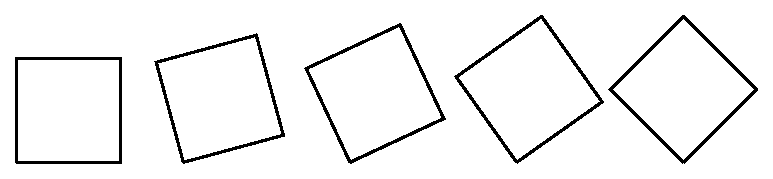
\includegraphics[width=5cm]{ChTurntitlePicture}
\end{center}
\item{\bold{Elementary Programming Concepts.}}
This part introduces the first programming concepts such as loops, variables... It presents how the messages sent to a robot are resolved. 
\begin{center}
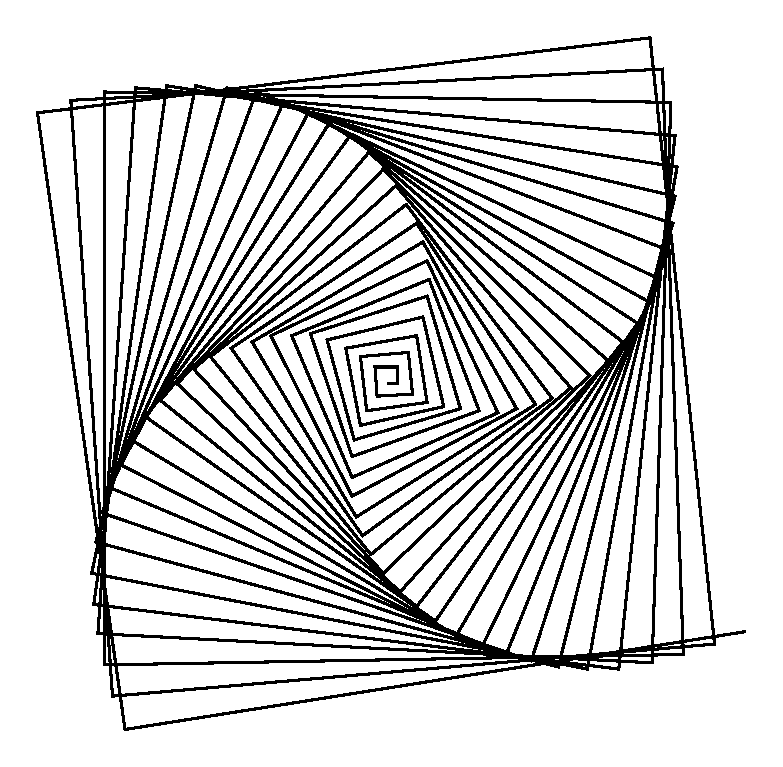
\includegraphics[width=4cm]{varLoopsTitle}
\end{center}
\item{\bold{Bringing Abstraction into Play.}} This part introduces the necessity of having abstraction \ie method or procedures that can be reused by different programs. The most difficult concept introduced is the idea of composing new methods from existing ones to solve more complex problems. Several non trivial experiments are proposed such as drawing golden rectangles. It introduces also techniques and tools to debug programs. 
\begin{center}
\includegraphics[width=5cm]{nborsteps}
\end{center}
\item{\bold{Conditionals.}} This part introduces the notion of conditional, conditional loops and booleans expressions that are central to programming. This part also introduces the notion of references in a 2D space and some other robot behavior. Then it presents how we can use a robot to simulate the behavior of simple animals. 
\begin{center}
\includegraphics[width=3cm]{followBorder2}\includegraphics[width=3cm]{oppositeBorderOfBox}
\end{center}

\item{\bold{Other Programming Environments.}}
This part presents two other environments available in \sq to have fun programming:  The eToy graphical scripting system is presented as well as Alice the 3D-authoring environment.
\end{description}


\section*{Why Squeak and Smalltalk?}

You may wonder why I use Smalltalk and why you would have a learn it in 2004 while a 
lot of other languages exist. I use Smalltalk and Squeak because:

\begin{itemize}
\item Smalltalk is a powerful language. We can build extremely complex systems and still the language is simple and uniform. 

\item Smalltalk was designed to be a language to teach programming. It was influenced by Logo and Lisp, and Smalltalk influenced heavily languages such as Java or C\# but these languages are overly complex and lost the beauty of Smalltalk its simple model. 

\item Smalltalk is dynamically typed and this makes transparent a lot of concerns related to types and types coercion that are tedious to explain for a really limited interest.

\item With Smalltalk you learn the key essential concepts that after you can find in all the other languages. With Smalltalk I can focus on explaining you the important concepts without having to deal with ugly aspects of certain languages. 


\item Squeak is a powerful multimedia environment, so after reading my books you will be able to build your own program in a really rich context. 

\item Squeak is free and runs on all the main platforms of today and can be ported to the ones of the future easily. 

\item Squeak is used in school in Spain on 80 000 computers. 
\end{itemize}

For all these reasons I choose Squeak. 



\section*{Thanks}
I would like to thanks all the people that read this book and gave feedback. I know this was not easy to read parts of a book on progress. I do not want to list you all here as I'm sure that I will forget people. However I want to thank the person who read the book entirely: Orla Greevy, Ian Prince and Daniel Knierim. I just want to thank you for your feedback and support. I have a particular thought to Daniel Villain who read the draft of the french version and died too early. 

I want to thank the Squeak community for the help it provided me during the development of the environments used in this book, and for developing Squeak this amazing environment. I have a special thank for all the developers that made Smalltalk escaping clouds of dream and becoming reality. I would like to thank all the Smalltalkers that make this language and community so exciting. Continue to make your dreams come true. 

Writing this book was a long and difficult process because teaching novices is difficult. Moreover I'm not an easy person to live with and a researcher that is excited by too much topics.  I want to thanks Didier Besset for the discussions we got even if at the end we were not synchronized.

I also  want to thank my wife Florence, and Quentin, and Thibaut  these two small boys that are running and shouting around my desk when I would like to be concentrated to accept a husband and father that is not always present, enthusiast and accessible. 

\ifx\wholebook\relax\else\end{document}\fi

  

\part{Getting Started}
%%%%%%%%%%%%%%%%%%%%%%%%%%%%%%%%%%%%%%%%

%1R
% Orla comments 20-Dec04
% Ian comments 20-Dec04
% TO BE UPDATED with latest pictures of the environment
% TODO: Dominic comments 20-Dec04

\ifx\wholebook\relax\else
\input{../Common.tex}
\input{../macroes.tex}
\begin{document}
\fi
	
\chapter{Getting Started}\label{ch:firstcontact}

The purpose of this chapter is that in five minutes from now you can be ready to use the environment you will use in this book. In this chapter you will learn how to install the  environment, understand the different parts of the environment and how to interact with the robots that live in this environment. You shall program these robots to accomplish challenging tasks by sending them messages.

Right now we just want to get you started and get ready for the rest of the book.   Note that if your environment is already installed then simply jump directly to the subsequent sections that explain the environment. Chapter~\ref{cha:caroTour} will explain in more detail the environment. 


%%%%%%%%%%%%%%%%%%%%%%%%%%%%%%%%%%%%%%%%%%%
\section{Installing the Environment}
The environment used in this book is developed on top of \sq. \sq is a rich and powerful open-source multimedia environment entirely written in Smalltalk and freely available for most of the computer and operating systems at http://www.\-squeak.\-org. Note however that you will not use directly a default  \sq distribution but use instead a distribution I prepared for you.  

\sq runs exactly the same on all the platforms, however to ease your start we prepared some platform dependent compressed files. The principle is exactly the same on Mac, PC, or any other platforms. Only the decompressing tools and the way to invoke \sq may differ. Once you have a file named \ct{ReadyToUse.zip}, you decompress it then drag the file named \ct{Ready.image} on the \ct{Squeak application}, and this is it! The file \ct{Ready} contains the complete environment used in this book

Now let us look at each of the steps one by one. Note that you may get files with slightly different names but it should work exactly the same.

\paragraph{On Macintosh.}
You should have a file named  \ct{readyToUseForMac.zip} a zipped archive. Normally double-clicking on the file should invoke the right decompresser such as StuffIt Expander. When you decompressed this file, you should obtain 4 files as shown by Figure~\ref{fig:macfiles}. You should identify two files: the file named \ct{Ready.image} and the \emph{Squeak application} file (the one without extension in Figure~\ref{fig:macfiles} it is named \ct{Squeak}).

\begin{figure}[h]\centerline{\includegraphics{readyToUseMacZip2}\includegraphics[width=9cm]{macFiles2}}
\caption{The files for the ready to use environment for Macintosh. Left: the zipped file. Right: the files.\label{fig:macfiles}}\end{figure}


\newpage


\paragraph{On Windows.}
You should have a file named \ct{readyToUse.zip}, an archive.  When you decompressed this file using Winzip, you should obtain 4 files as shown by Figure~\ref{fig:pcfiles}. You should identify two files: the file named \ct{Ready.image} and the \emph{Squeak application} file (the one without extension in Figure~\ref{fig:pcfiles} it is named \ct{Squeak}.


\begin{figure}[h]\centerline{\includegraphics{zipPC}\includegraphics[width=9cm]{readyPC}} 
\caption{The files for the ready to use environment on PC. Left: the zipped file. Right: the files.\label{fig:pcfiles}}
\end{figure}


\section{Opening the Environment} 
To open the environment, drag the file \ct{Ready.image} on the \emph{Squeak application} that is the file named Squeak as shown by Figure~\ref{fig:dropImage}. You should get the environment shown in Figure~\ref{fig:firstEnvironment}. If you do not get this environment then read Section~\ref{sec:trouble}.

\begin{figure}[!h]\centerline{\includegraphics[width=8cm]{dropImage2}  \includegraphics[width=8cm]{readyDD}} 
\caption{Dragging and dropping the \textit{image} file on the 
\textit{Squeak application} to open on Mac (left) on PC (right).\label{fig:dropImage}}
\end{figure}

\paragraph{Hints.}
The environment can be opened by simply double-clicking on the \textit{image} file. However, such a practice has several disavantages: you may have to identify the \emph{Squeak application} and sometimes another application may by accident try to use the image. Moreover it can lead you to trouble when you have multiple installations of different versions of \sq. So we suggest to always open the environment by dragging and dropping the \emph{image file} on the \emph{Squeak application} file or alias to it. Note that if you have space problem you can use an alias to the SqueakV3.sources file as this file can be shared between multiple installations. 

\begin{largecadre}{To start the environment. 
Drag and drop the file terminating with the .image extension into the squeak application.}
\end{largecadre}
 
%%%%%%%%%%%%%%%%%%%%%%%%%%%%%%%%%%%%%%%%%%%
\section{First Interactions with a Robot}

Once you open the environment by dragging the file named \ct{Ready.image} on the Squeak executable as explained previously, you should obtain an environment similar to the one presented by Figure~\ref{fig:firstEnvironment}. 


\begin{figure}[!h]\centerline{\includegraphics[width=10cm]{firstEnvironmentAnnotated}} 
\caption{The environment ready to use.\label{fig:firstEnvironment}}
\end{figure}

The environment is composed of robot factories and two flaps. A flap is a drawer containing programming tools that you do not need to use now and we will describe later in Chapter~\ref{cha:caroTour}. Now you should see a small blue robot in the middle of the screen. Of course this is not a physical robot, but a software robot seen from above pointing on the right of the screen.  A robot is a round blue circle; it has two catterpilars and a small red head indicating its current direction. In this book you shall send orders to robots, we say that we send them \emph{messages} \index{messages} and robots execute these messages.

Place the mouse over the robot and wait a second there. A balloon pops up with some information about the robot such as its current location and its direction as shown in Figure~\ref{fig:firstBalloon}. As your screen is of different size than the one used to produce this book, you may have other values.  

\begin{figure}[!h]\centerline{\includegraphics[width=8cm]{firstBalloon2}}
\caption{Place the mouse over a robot to get a balloon showing some information related to the robot in question.\label{fig:firstBalloon}}
\end{figure}

\paragraph{Sending Messages to a Robot.}
To interact directly with a robot by left-clicking on the robot with the mouse.  A messaging balloon pops up as shown by the left picture of Figure~\ref{fig:go}.  You can type some messages that are sent to the robot. Once you typed these messages, hitting the \bold{return} key actually sends them to the robot which will then execute them.

\begin{figure}[h]\centerline{\includegraphics[width=16cm]{sendingAMsg2}}
%emptyBalloon}\includegraphics{go}\includegraphics{gone}}
\caption{Step 1: left-clicking on a robot produces a balloon to send a message to a robot. Step2: Typing a message to ask a robot to move forward. Step 3: the robot moved and left a trace on the ground.\label{fig:go}}
\end{figure}

\begin{figure}[!h]\centerline{\includegraphics{turn20+702}\hfill\includegraphics{turned2}}
\caption{Left: Sending a complex message. Right: Its effect.\label{fig:turned}}
\end{figure}

 For example by typing the message \ct{go: 200} and hitting the return key, we ask the robot to move forward 200 pixels in its current direction, or typing the message \ct{turnLeft: 20 + 70} we ask the robot to turn on its left of 90 degrees. The message \ct{color: Color green} changes the color of the robot as shown by the Figure~\ref{fig:green}.

As the messages show, we can write complex messages and we will explain how you can write such messages later. For now simply type what we show you. Note that if you want to repeat some expressions, you do not have to retype them but simply use the up and down arrows to navigate over the previous messages you sent to the robot. In the subsequent chapters, you shall learn step by step all the messages that a robot understands and more important you shall learn how to define new behavior for your robots.





\begin{figure}[!h]\centerline{\includegraphics{colorGreen2} \hfill\includegraphics{green2}}
\caption{Left: Changing the color of a robot to another color. Right: its effect \label{fig:green}}
\end{figure}


\begin{largecadre}{To interact with a robot. Click on it, type the message and hit the \bold{return} key.}
\end{largecadre}

%%%%%%%%%%%%%%%%%%%%%%%%%%%%%%%%%%%%%%%%%%%
\section{Creating a New Robot}
The environment already contains a robot but now we show you how to create new robots. To create a new robot we ask a robot \emph{factory} to create a new one. A robot factory is graphically represented by an orange box surrounded by a blue light box in the middle of which the word Bot is written as shown in Figure~\ref{fig:classBalloon}. A robot factory \index{robot factory} is called in \sq jargon a \index{class} \emph{class}.
Classes (object factories) have a name starting with an uppercase letter. Hence this is the class \ct{Bot} and not \ct{bot}.  

As for robots, we interact with a robot factory by sending it messages. The message to create a new robot is the message \ct{new} as shown in Figure~\ref{fig:turtleBoxNew}. 
Note that newly created robots point also to the right of the screen. Now you can send messages to the two robots individually, each of them living its own life. 

\begin{figure}[!h]\centerline{\includegraphics[width=8cm]{classBalloon2}}
\caption{A robot factory called in \sq jargon a \emph{class}. It produces new robots. \label{fig:classBalloon}}
\end{figure}

\begin{figure}[!h]\centerline{\includegraphics[width=14cm]{creatingARobot2}}
%{turtleBoxNew} \includegraphics{newTurtleInHand}}
\caption{Step 1: Start to type a message. Step 2: sent the message \ct{new} to the factory to get a new robot. Step3: The factory creates a robot and gives it to you.\label{fig:turtleBoxNew}}
\end{figure}

\begin{largecadre}{To create new robots. Send the message \ct{new} to the robot factory, a class.}
\end{largecadre}

When a robot is created, it is always pointing to the east or the right of the screen. 


%\section{Getting an Animated Robot}
%The robot with which you just interacted was not animated \ie you could not see how the messages were performed. Sometimes it would be nice to see the robot executing the messages step by step. This is possible. For this you have to create an animated robot by sending the message \ct{new} to the class \ct{AniBot} as you did previously to get new robots. The new robot you get understands all the messages a basic robot understands. 
%Animated robots are green to distinguish them from basic ones. Send some messages to the robot to see it performing them.

%\begin{figure}[!h]\centerline{\includegraphics{aniTurtleClassNew}\includegraphics{aniTurtle}}
%\caption{Left: Asking the animated robot factory to create a new robot. Right: Getting a new animated robot. \label{fig:animated2}}
%\end{figure}

%%\begin{figure}[!h]
%%\begin{center}
%%\centerline{\includegraphics{aniTurtleNewInBalloon}}
%%\caption{Creating an animated turtle.\label{fig:animatedcreated}}
%%\end{center}
%%\end{figure}

%Note that if the animation speed is too slow you can change it using the message \ct{speed:} and providing a number such as 1000 or 10000. For example, type in the balloon \ct{speed: 10000} to test it.  



%%%%%%%%%%%%%%%%%%%%%%%%%%%%%%%%%%%%%%%%%%%
\section{Quitting and Saving}\label{sec:quit}

The background of the \sq window application is called the \index{world} World. The World has a menu offering a lot of functionality. To display the World menu just click on the background. You should get a menu similar to the one shown in Figure~\ref{fig:worldMenu}. The last group of elements are all the actions you can do to quit or save your work. 

\begin{figure}[!h]
\center{\includegraphics[width=8cm]{worldMenuAnnotated}}
\caption{The World menu.\label{fig:worldMenu}}
\end{figure}

Selecting the item 'quit' simply quit without saving what you did. Therefore the next time that you will restart the environment it will be exactly in the same state as when you started this time. Selecting the item 'save', save the complete environment. The next time you till start it, it will be exactly in the same time that at the moment you saved it. 
Finally when selecting the item 'save as...',  the environment asks you to give a new name and it will create two new files with that name: one with the extension \ct{.image} and one with the extension \ct{.changes}.  This is this way that we created the files \ct{Ready.image} and \ct{Ready.changes}.  To open the environment you saved with a new name, drag and drop the file with the new name which has the extension \ct{.image} on the squeak executable as you did to start the environment by dragging and dropping the file \ct{Ready.image}.





\section{Possible Installation Troubleshootings}\label{sec:trouble}
Now we try to help to fix the problems you may encounter during the installation. For that we will explain the role of each important files you got once you decompressed the archive.

To run the environment provided with this book or any  \sq distribution, four files are necessary. We describe them now as we will use their name to help solve the possible problems you may encounter.  The four files are: 
\begin{description} 
\item[Image and changes.] The file named \ct{Ready.image}, called simply the \textbf{image}\index{image file} file and the file named \textbf{Ready.changes}, called simply the \textbf{changes} \index{changes files} file contain the information of your current system. These two files are synchronized by \sq automatically and \emph{should be writable}. Each time you save you environment they are synchronized. You should not edit then with another file editor or changes the name of the file manually. If you want to have different names, just use the \menu{save as ...}
menu item of the World menu, \sq will then create a new pair of files for you. 

 
\item[Source.] The file named \ct{SqueakV3.sources}, also called \textbf{sources}\index{sources file}, contains the source of a part of the \sq environment. You do not need it in this book so do not try to edit manually. However, this file should always be in the directory in which the image is.
  
\item[Application.] The application Squeak for mac or Squeak.exe for PC is the \sq system. This is this application that runs when you program in \sq. It should then be executable. We refer to this file as the \index{Squeak application}\textbf{Squeak application}. In computer scientist jargon, this application is called a \index{virtual machine} virtual machine called or  a VM \index{VM} in short. 
\end{description}

As we already mentioned it the \textit{image} and \textit{changes} files should be writable. Certain operating systems change the properties of the files to read-only when copied from a CD. In such a case, \sq warns you with a message as shown in Figure~\ref{fig:readonlyfile}. If you get this message, simply quit \sq without saving, change the property of the file to be writable and restart.  

\begin{figure}[!h]\centerline{\includegraphics[width=\linewidth]{changesNotWritable}}\caption{The error message showing that
 the image (\ct{Ready.image}) or changes (\ct{Ready.changes}) files are not writable.\label{fig:readonlyfile}}
\end{figure}

Another possible problem you may encounter is related to the sources file named \ct{SqueakV3.sources}, this file or an alias to this file should be present in the directory where the image file is. When this file is not present you may get on Mac the first message shown in Figure~\ref{fig:sourcesMissing} (note that this message is not clear and refers to a problem related to aliases that is fixed in the current version of \sq) or the second message. To cure this problem, create an alias to the source file (\ct{SqueakV3.sources}) into the directory containing  your image or simply copy the sources file  to be in the same directory that the image file.

\begin{figure}[!h]%\center{\includegraphics{sourcesMissing}}
\center{\includegraphics[width=\linewidth]{sourcesMissing2}}\caption{Some possible error messages indicating that the \textit{source} file (\ct{SqueakV3.sources}) is missing in the directory containing the \textit{image} file .\label{fig:sourcesMissing}}
\end{figure}





%%%%%%%%%%%%%%%%%%%%%%%%%%%%%%%%%%%%%%%%%%%
\summa

\begin{itemize}
\item To start the environment, drag and drop the file terminating with the .image extension into the squeak application.

\item To send a message to a robot, left-click on it, type the message and hit the \bold{return} key.

\item To create new robots. Send the message \ct{new} to the robot factory, a class.
%\item  In an interaction balloon the word \ct{self} refers to the robot receiving the message.

\item When a robot is created, it is always pointing to the east or the right of the screen. 

\item The background of the environment is called the World.

\item To get the menu to save the environment, click on the background close to a robot.
\end{itemize}



\ifx\wholebook\relax\else\end{document}\fi



 %O+I + Dominic =>  TD figures
%2R
%Orla + Ian 20 dec 04
% 27 Dec: comments of dominic
%TD: update picts

\ifx\wholebook\relax\else
\input{../Common.tex}
\input{../macroes.tex}
\begin{document}
\fi

%%%%%%%%%%%%%%%%%%%%%%%%%%%%%%%%%%%%%%%%%%%
%%%%%%%%%%%%%%%%%%%%%%%%%%%%%%%%%%%%%%%%%%%
\chapter{A First Script and its Implications}\label{cha:firstscript}

While sending messages using direct interaction with a robot is a fun and powerful way of programming robots, it is a bit of a limited way to write more complex programs. Therefore you shall learn the notion of \emph{script}, \ie a sequence of expressions and all the necessary concepts that you will use in this book. Hence, this chapter settles down the vocabulary for the rest of the book. It also serves as a map to the next chapters that will introduce in depth the concepts briefly presented in this chapter.
 
First I present how you to send multiple messages to the same robot separating messages with a semi colon. Then you shall learn how to write script using a dedicated tool called a \index{workspace} workspace. I will describe the different elements that compose a script and  present the possible mistakes that can happen when writing programs.
 
%%%%%%%%%%%%%%%%%%%%%%%%%%%%%%%%%%%%%%%%%%%
\section{Using a Cascade to Send Multiple Messages}
Start to draw a rectangle of 200 height on 100 width. To do so you will start to type the first message \ct{go: 100} hit the return key then click on the robot and type the second expression \ct{turnLeft: 90} and hit the return key, then click on the robot and type the expression \ct{go: 200}... As you quickly notice it this is really tedious. What would be much more handy would be to be able to type everything in one shot and that it gets executed. 

You can send multiple messages to a robot by separating them with  a semi-colon \ct{;}.  To send to a robot  the messages \ct{go: 100}, \ct{turnLeft: 90}, and \ct{go: 200}  simply separate them with a semi-colon \ct{;} as follows \ct{go: 100 ; turnLeft: 90 ; go: 200} (see Figure~\ref{fig:cascading}). This way of sending multiple messages to the same robot is called a \index{cascade}\emph{cascade} of messages in \sq jargon. 

\begin{figure}[!h]
\center{\includegraphics[width=10cm]{goturnleftgo2}}
\center{\includegraphics[width=\linewidth]{goturnleftgoLong2}}
\caption{Sending several messages in one shot to a robot using \ct{;}. \label{fig:cascading}}
\end{figure}

However, using a cascade (that is sending multiple messages to a robot separated by the character \ct{;}) does not work well for complex programs. Indeed even for a drawing a simple rectangle is it too long as shown by the second message in Figure~\ref{fig:cascading}. In addition, there are other concerns that professional programmers take into account such as if they can store the sequences of messages and replay them later, whether they can reuse them and not have to type them all the time. For all these reasons, we need other ways to program robots. The first way is to write the sequence of messages, that is called a \emph{script},  in a text editor and ask the environment to execute them as you shall see in a minute. 

\section{A First Script}
The BotInc environment provides a small text editor, called the \tw which is dedicated to script execution (that is executing of the expressions composing a script). Click on the bottom flap called \textbf{Working}, by default it contains a \tw editor as shown by Figure~\ref{fig:TurtleWorkspace}. 

\begin{figure}[!h]
\center{\includegraphics[width=10cm]{TurtleWorkspace}}
\caption{A \tw is a small editor dedicated to the execution of robot scripts. \label{fig:TurtleWorkspace}}
\end{figure}

Let us define a first script  that draws a rectangle and explain it in detail (\scrref{scr:firstScript}).  Figure~\ref{fig:doit} shows the script in a \tw and the result of its execution  obtained by pressing the \button{Do It All} button. Try to get the same result: type the script and press the \button{Do It All} button. Note that I use \ct{pica} as a nickname of picasso since our robots are drawing pictures. 


\begin{scriptwithouttitle}\label{scr:firstScript}
| pica |
pica := Bot new.
pica go: 100.
pica turnLeft: 90.
pica go: 200.
pica turnLeft: 90.
pica go: 100.
pica turnLeft: 90.
pica go: 200.
pica turnLeft: 90
\end{scriptwithouttitle}


The \button{Do It All} button of \tw executes \emph{all} the messages it contains, therefore before typing a script make sure that no other text is already present in the \tw.  Moreover, computers and programming languages cannot deal with even the most obvious mistakes, so be careful to type the text exactly as it is presented in \scrref{scr:firstScript}. Pay attention to type the  \index{class name} uppercase "B" of \ct{Bot} on the second line and to end  each line with \index{dot}\index{period}\index{message separator} a \period. There is no need to put a \period at the end of the last line because there is no other messages to send to the robot.


\begin{figure}[!h]
\center{\includegraphics[width=10cm]{fsdoit}}
\caption{A script executed using the \button{Do It All} button of the \tw and its result.\label{fig:doit}}
\end{figure}






\section{\sq and \st}
As you see the script you typed is simple but still it constitutes a program. A program is a list of expressions that a computer can execute. To define programs we need programming languages, \ie languages that allow programmers to define programs that a computer can understand and execute.

\subsection*{Programming Languages}
The idea behind a programming language is to support programmers to express
 solutions to their problems. Support means various things like ease of expression
of the task, efficient execution of the program, reliability of the
resulting application, proof that the program is correct, readibility
of the code written, ease to change the application later on \ldots  There
is no \emph{per se} best language that satisfies all these properties. Programming
languages exhibit different expressive power and properties.

In this book you shall learn how to program in the \st programming language in the \sq environment. \st is a object-oriented programming language like Java or C++. 

\subsection*{\st and \sq}
\sq \index{Squeak} is the name of a \index{programming environment} programming environment. A programming environment is a set of tools that programmers use to
develop applications. \sq contains a lot of tools: text editors,
code browsers, a debugger, an object inspector, a compiler, widgets.... Moreover, \sq contains a lot more for example, you can program music, animate flash files, access the networks, display 3D objects...and much more! However before you can start programming complex applications you have to learn some basic principles and this is the purpose of this book.

\sq programmers develop their applications by writing programs using the
programming language called \index{Smalltalk}\st. \st  is an \emph{object-oriented} language.  This means that objects are created --- virtual objects within the computer, of course --- and these objects are able to understand \index{message} messages that they execute when they receive them. However in the context of this book we will not show you how to define new classes, you will only define new behavior for your robot because object-oriented programming is a bit complex and you have to learn basic programming concepts first.

We chose \st because it is simple, uniform and pure: in \st everything is an object that send messages to other objects and receive messages. In \st there are simple rules and they are always applied consistently. In addition, \st was originally designed for teaching novices how to program. Note that even if \st was designed for novice programmers in mind, large and complex applications have been written in Smalltalk such as the applications controlling the machines that produce the AMD micro-processors that you may have on your current computer. 

Finally, a really interesting aspect of \sq is that it completely written in \st. This implies that if you understand \st you can change, adapt the system to your own needs or 
learn from the system. With \st you have a lot of power in your hands. I hope that you get motivated to learn how to program, but watch out programming like playing piano or painting is not simple, therefore do not be discouraged if you get some difficulties, this is normal and I designed this book so that topics get introduced one after the others smoothly.

\section{Programs, Expressions and Messages}
Now we are ready to take a closer look at your first script and explain it. 
 
\subsection{Typing and Executing Programs}
Let us start by looking at the way you wrote your first script or program (\scrref{scr:firstScript}). You typed a text, a sequence of \emph{expressions}, then you asked \sq to execute it by pressing the \button{Do it All} button. \sq executed the sequence of expressions, that is, it transformed the textual representation of your program into a form that is understandable by a computer, then each expression was performed one after the other. In the first script, the execution created a robot and the robot executed one after the other the messages that were sent to it. 

A program consists of a sequence of \textit{expressions} that are executed by the \sq environment. In this book, we call such a sequence a \index{script} \emph{script}.
  
\largecadre{Vocabulary Point. We called a \emph{script} a sequence of expressions.} 
  
A program is a bit like a cooking recipe. A recipe describes all the steps to cook a meal. A program describes all the steps to produce a certain effect. For example to cook pancakes, the expressions are all the steps we should do to prepare them: mix flavor and milk, add the eggs, heat the pan, etc...

\subsection{Anatomy of a Script}
Now comes the time to understand your first drawing script that I copy here (\scrref{scr:firstScript2}):

\begin{scriptwithouttitle}\label{scr:firstScript2}
| pica |
pica := Bot new.
pica go: 100.
pica turnLeft: 90.
pica go: 200.
pica turnLeft: 90.
pica go: 100.
pica turnLeft: 90.
pica go: 200.
pica turnLeft: 90
\end{scriptwithouttitle}


In a nutshell, the script~\ref{scr:firstScript2} declares that it uses a variable named \ct{pica}  to refer to the robot it creates. Once the robot is created and associated with the variable \ct{pica} the script asks the robot to move to different locations on the screen.  Now let us analyze each line step by step even if certain concepts such as variables will be treated in separate chapters.
  
\begin{description}
\item[\ct{| pica |}] This first line declares a variable. It tells \sq that we want to use the name pica to refer to an object.  Think of it as saying to a friend, from now on I will use the word pica in my sentences\index{variable definition}\index{bar@\texttt{"|}|see{vertical bar}} to refer to a robot. You shall learn more on variables in Chapter~\ref{ch:variables}.

\item[\ct{pica\ :=\ Bot\ new.}] This line creates a new robot by sending the message \ct{new} to the robot class named \ct{Bot} and  associates it with the name \ct{pica}, the variable that we declared before. The word \ct{Bot} requires an uppercase letter \ct{B} because it is a class, that is a factory of robots\index{robot creation}\index{instance creation}.
    
\item[\ct{pica go: 100.}]  The message \ct{go: 100} is sent to the robot we named \ct{pica}. This line can be understood as follows: "pica, move by 100 units of length on the screen". Note that  any message name that terminates by a colon indicates that this message needs additional information, such as a length or an angle. For example, \ct{go: 100} says that the robot should move 100 pixels. The message name is \ct{go:}.

\item[\ct{pica turnLeft: 90.}] This line asks pica to turn 90 degrees  on its left. This lines is again a message sent to the robot named pica.
  
\item The other lines are just repetitions of the previous ones, 
so they have the same effect.
\end{description}




\largecadre{Any \textbf{message} name that terminates by a colon indicates that this message needs additional information, such as a length or an angle. 
\\ \\
For example, the message name \ct{turnLeft:} requires a number representing the angle from which the robot should turn.}

\paragraph{About Pixels.} On a computer screen the unit of distance is called a
\index{pixel}\strong{pixel}. A pixel is the size of the smallest
point which can be drawn on a computer screen. Depending on the type
of computer you are using the actual size of a pixel can vary. You can
see pixels by looking at the screen through a magnifying glass.




%%%%%%%%%%%%%%%%%%%%%%%%%%%%%%%%%%%%%%%%%%%
\subsection{Expressions, Messages and Methods}
Now I should clarify some vocabulary points.

\paragraph{Expression.}
We call an expression\index{expression} any element of a program. Here are some examples of expressions: 

\begin{itemize}
\item \ct{| pica |} is an expression that declares a variable (see Chapter~\ref{cha:variables}).
\item \ct{pica := Bot new} is an operation, called  assignment,  that associates a value to a variable (see Chapter~\ref{ch:variables}). Here, the newly created robot obtained by sending the message \ct{new} to the class \ct{Bot} is associated to the variable \ct{pica}.
\item \ct{pica go: 100} is a message send. The message \ct{go: 100} is sent to  \ct{pica}.
\item \ct{100 + 200} is a message send. The message \ct{+ 200} is sent to  \ct{200}.

\end{itemize}




\begin{figure}[h]
\begin{center}\includegraphics{message}
\caption{Two messages composed of  a message name or method selector, and a set of arguments.\label{fig:firstScriptMessage}}\end{center}
\end{figure}

\paragraph{Message.}
We call a \index{message}\strong{message}, a pair composed of a \strong{message name}\index{selector} also called a \strong{message selector}, and \strong{message arguments}, the required values to execute the message  as shown by Figure~\ref{fig:firstScriptMessage}. A message is sent to a \index{receiver}\strong{message receiver}. \\

\noindent
Example of messages are:
\begin{itemize}
\item In \ct{pica beInvisible}, the message \ct{beInvisible} is sent to a receiver, a robot. This message does not require arguments.

\item In \ct{pica go: 100}, the message \ct{go: 100}  is sent to a receiver a robot. It is composed of the method  name \ct{go:}, and an argument the number \ct{100}. Here, \ct{100} represents the length in pixels of which the robot should move.  Note
that the colon is part of the method selector.

\item In \ct{33 between: 30 and: 50}, the message \ct{between: 30 and: 50} is composed of  the method selector \ct{between:and:}, and two arguments \ct{30} and \ct{50}. This method checks whether the receiver, a number, is between two values, here the numbers \ct{30} and \ct{50}.

\item In \ct{4 timesRepeat: [ pica go: 100 ]}, the message \ct{timesRepeat: [ pica go: 100 ]} sent to the number 4, is composed of  the method selector \timesRepeat, and the argument \ct{[ pica go: 100 ]} a block, a sequence of messages (see Chapter~\ref{ch:looping}).

\item In \ct{100 + 200}, the message \ct{+ 200} is composed of the method selector \ct{+}, and an argument, the number \ct{200}. The receiver is the number \ct{100}.
\end{itemize}



\paragraph{Message separation.}
You have noticed that each line of the script~\ref{scr:firstScript}, except the first one, is terminated by a \period. As we have said earlier, the first line is not a message. Such a line is called a \index{variable declaration} variable declaration in computer jargon. Thus, we can make the following observation: each message must be separated from the following one by a \period. Note that putting a \period after the last message is possible but not mandatory: \st accepts both.

\largecadre{Messages should be separated by a \period. The last statement does not require a terminal \period.

\begin{nalltt}
pica := Bot new.\\
pica go: 100.\\
pica turnLeft: 90.\\
pica go: 100
\end{nalltt}}

\paragraph{Hints.} A \period \ct{.} is a \index{message separation} message \textit{separator} so there is no need to put one if there is no message after it like at the end of a script or a sequence of messages.


\paragraph{Method.}
When  a robot receives a message it executes a \emph{method}\index{method} which is kind of script that has a name.  A method is a named sequence of expressions that a receiver executes in response to a message. For example, the method \go makes the receiver going a certain number of pixels in its current direction. This method \go is executed when a robot receives a message whose name is \go. In the future, I will explain to you how to define new methods for your robot but for now we do not need them to start programming.



\subsection{Using the Cascade}
As I mentioned in the first section of this chapter, you can send multiple messages to the same robot by separating them with a semi-colon, called a cascade. 
In a script, we can also use a cascade (\ct{;}) to send multiple messages to the same robot. \scrref{scr:firstScript2} is equivalent to the following one (\scrref{scr:firstScriptsemi}) where all the messages sent to the same robot are separated by a semi-colon. Using cascades is handy  when you want to avoid to type the receiver of the multiple messages. The cascade is interesting because it shortens scripts. However pay attention that you understand clearly that all the messages are sent to the same receiver.

\begin{scriptwithouttitle}\label{scr:firstScriptsemi}
| pica |
pica := Bot new.
pica 
   go: 100 ; turnLeft: 90 ; go: 200 ; turnLeft: 90 ; 
   go: 100 ; turnLeft: 90 ; go: 200 ; turnLeft: 90.
\end{scriptwithouttitle}



\begin{largecadre}{To send multiple messages to a Bot use a semi-colon \ct{;} to separate the messages, following the template: \ct{aBot message1 ; message2}. \\ \\
For example, \ct{pica    go: 100 ; turnLeft: 90 ; go: 200 ; turnLeft: 90}}
\end{largecadre}

\subsection{About Robot Creation}

To get a new robot you have to send a message, the message \ct{new} to the \emph{class} \ct{Bot}. Note that this is not new! This follows exactly what you did in the previous chapter where you clicked on the blue and orange box named \ct{Bot} representing the class of the same name and typing \ct{new} in the bubble. In \sq, we \emph{always} send messages to objects, robots or classes to interact with them. There is no difference in treatment, except that class and objects understand different messages. Indeed, an object does not know how to create other objects so sending to a robot the message \ct{new} leads to an error and sending the message \ct{color} or \ct{go:} to a class does not make sense and leads naturally to an error. Still in both cases you are sending messages!

Note that other class may provide other messages to create objects such as the class \ct{Color} which returns the color blue or green in response to the messages \ct{blue} or \ct{green}. Do not worry I will always let you know how to get objects of specific classes. 

\largecadre{To get a new object, send the message \ct{new} to a class. \ct{Bot new} creates a new robot. Other classes may offer different messages to get new objects. For example, \ct{Color blue} asks the class \ct{Color} to create a new  color been blue.}

\section{Possible Errors while Writing Programs}
Computers are capable of making highly complex calculations at incredible speed, but they lack the intelligence to correct small mistakes. This means that each expression given to a computer must be given without mistake. The smallest mistakes --- even a lowercase letter instead of an uppercase one --- are likely to be misunderstood by a computer.  In that case, an error message will appear on the screen. This is likely to occur when you are doing your first experiments. So do not despair and try to understand what went wrong. 


\begin{figure}[ht!]
\begin{center}\includegraphics[width=6cm]{errorOne}
\caption{We mispell the message \ct{go:} and type \ct{god:} instead. The message \ct{god:} does not exist therefore \sq prompts us. \label{fig:unknowSelector}}\end{center}
\end{figure}

\sq colors the letters while you are typing, when a word is getting red, this means that you are writing something that \sq does not know. When a word is blue, for a variable or a message, or black for a class, this indicates that everything is correct. In addition, when we execute a message containing an error,  \sq tries to help you by notifying you when it encounters error in the code you wrote.  The error messages that \sq use are in fact menus. The top part in turquoise of the menu window contains a short description of the error; then, depending on the type of error some suggested corrections may be listed as options. Note that you can always cancel  the execution by choosing the cancel choice in the menu and in such a case you must find the place that the computer did not understand, correct it, and retry to execute the script. Here are the most common errors.






\paragraph{Mispelling a message.} You can misspell the name of a message.  In Figure~\ref{fig:unknowSelector} I misspelt the message \ct{go:} and typed \ct{god:} instead.  The message \ct{god:} did not exist therefore \sq turned the word in red. When I tried to execute the script, \sq prompted me. \sq tried to guess what is the message name I wanted to write and it proposed me several messages. I can pick the right message (\ct{go:}) and the message \ct{god:} will be replaced by \ct{go:} or I can simply chose cancel. In that case I will have to change manually \ct{god:} into \ct{go:}.


\begin{figure}[h]
\begin{center}\includegraphics[width=7cm]{mispellVariable}
\includegraphics[width=7cm]{unknowVariable}
\caption{Two examples of error. We mistyped the names of the variable. First in the script \ct{pica1} has not been declared and second while defining the variable: \ct{car o} defines two variables \ct{pic} and \ct{a} but not a variable \ct{pica}. \label{fig:wrongVar}}\end{center}
\end{figure} 

\paragraph{Mispelling a variable.} There are two ways to mispell a variable during its declaration (between the two vertical bars \ct{|}) or in the script itself. Figure~\ref{fig:wrongVar} shows the two cases: in the top case I typed \ct{pica1} instead of \ct{pica} in the script. \sq proposed me to define \ct{pica1} as a new variable or to replace \ct{pica1} by \ct{pica}. In the present case choosing \ct{pica} is the solution as shown by Figure~\ref{fig:wrongVar}. The bottom case shows that I misspelt the variable \ct{pica} during its declaration. In fact the space in the middle has for effect to define two variables \ct{pic} and \ct{a}. \sq saw that \ct{pica} was not declared and then it proposed me to declare a new variable with this name or to use the variable \ct{pic}.


\paragraph{Unused variables.} It may happen that we declare too many variables. Even if this is not an error, \ie the program can still run correctly. \sq checks this for us and proposes that we remove the unused variables. For example, in Figure~\ref{fig:unusedVariables} the script only uses the variable \ct{pica} and not \ct{pic} and \ct{a}. Therefore \sq prompts us to remove those. 

\begin{figure}[h]
\begin{center}\includegraphics[width=7cm]{unusedVariables}
\caption{All the variables and messages are correct. However the variable \ct{daly} is  defined but not used so \sq indicates it to us. Unused variables are not a problem so you can proceed.\label{fig:unusedVariables}}\end{center}
\end{figure}

\paragraph{Forgetting an uppercase.} Another common mistake is to forget uppercase when needed. Uppercase is needed when you want to send message to object factories. Figure~\ref{fig:TMissing} shows that I typed \ct{bot} instead of \ct{Bot}. \sq tried to find a solution but it fails. In such a case you have to correct it yourself. In the context of this book you only have to pay attention to put an uppercase for \ct{Bot} the robot factory, \ct{Color} the factory of colors.


\begin{figure}
\begin{center}\includegraphics[width=7cm]{BMissing}
\caption{We forgot the uppercase B  to indicate that we want to send a message to the class (the robot factory). We should correct it. \label{fig:TMissing}}\end{center}
\end{figure}


\paragraph{Forgetting a \period.} Finally one of the most common mistakes that even fluent programmers make, is to forget a \period or a cascade between two messages. In such a case \sq thinks that the following variable is just another message and tries to correct it. For example in Figure~\ref{fig:periodMissing} a \period is missing after the expression \ct{pica := Bot new} therefore \sq tries to send the message \ct{pica} and this message does not exist, therefore it tries to propose a replacement but failed to find. In such a case, you have to cancel and type the \period manually.

\begin{figure}[h!]
\begin{center}\includegraphics[width=6cm]{periodMissing}
\caption{Two examples of error. We mistyped the names of the variable. First in the script \ct{pica1} has not been declared and second while defining the variable: \ct{car o} defines two variables \ct{car} and \ct{o} but not a variable \ct{pica}. \label{fig:periodMissing}}\end{center}
\end{figure} 

\paragraph{About Colored Words}
\sq tries to identify mistakes when you are typing your scripts and it provides some visual clues on the possible errors. Figure~\ref{fig:coloring} shows some typical situations: 
\begin{itemize}
\item{(a)} I started to type the first letter of an undeclared or unknown variable. As there is no variable starting with the letter x, \sq turned the x in red, letting me know that I was doing a mistake. 
\item{(b)} I finished to typed a variable which is declared, therefore \sq turns it into blue to let me know that the variable is declared. 
\item{(c)} I'm writing a variable whose beginning is the one of a declared variable so \sq underline it to let me that I'm going well. 
\item{(d)} As soon as I type a character that leads to a variable that is not declared, \sq turns it in red. Note the difference with the previous case. In case (c) I could have typed the character a and then completed the word pica as in (a), I typed the character b and ended up with a undeclared variable (\ct{picb}). 
\item{(e)} After having typed the name of a declared variable (as in case (b)), I added an extra character a and this leads to the name of an unknown variable (\ct{picaa}).
\item{(f)} \sq tries to do the same for the message names. Here I misstyped the message \ct{go:} and typed instead \ct{gou}. As soon as I typed the character u, \sq saw that the message name \ct{gou} was unknown so it turned it in red. 
\item{(g)} \sq tries to  do the same for the classes. Here I typed the character w after Bot and \sq indicates to me that there is no class named \ct{Botw} in the system.
\end{itemize}


\begin{figure}[h!]
\begin{center}\includegraphics[width=12cm]{coloring}
\caption{\sq using colors to help finding mistakes. \label{fig:coloring}}\end{center}
\end{figure} 




\summa
\begin{itemize}
\item \emph{To execute an expression}. Press the \button{Do It All} button of the workspace.




\item A \emph{script} is a sequence of expressions that perform a task.

\item A message is composed of a message name, and some arguments. Some message may not required arguments. For example \ct{pica beInvisible} 

\item Any message name terminated by a colon indicates that this message needs additional information, such as a length or an angle for example. For example, the message name \ct{turnLeft:} requires a number representing the angle from which the robot should turn.

\item To get a new object, send the message \ct{new} to a class. \ct{Bot new} creates a new robot. Other classes  may offer different messages to get new objects. For example, \ct{Color blue} asks the class \ct{Color} to create a new  color been blue.


\item A class is a factory of objects. Class names always start with an uppercase letter. Here \ct{Bot} is the factory creating new robots and \ct{Color} the one creating colors. \

\begin{nalltt}
Bot new color: Color blue
\end{nalltt}

\item Messages should be separated by a \period. Terminal \period is not required.\

\begin{nalltt}
pica := Bot new.
pica go: 100.
pica turnLeft: 90.
pica go: 100
\end{nalltt}


\item To send multiple messages to the same object use a semi-colon \ct{;} to separate the messages, following the template: \ct{aBot message1 ; message2}. For example, \ct{pica    go: 100 ; turnLeft: 90 ; go: 200 ; turnLeft: 90} send the message \ct{go: 100}, \ct{turnLeft: 90}, \ct{go: 200}, \ct{turnLeft: 90} to the same robot named \ct{pica}.
\end{itemize}







\ifx\wholebook\relax\else
\end{document}\fi







\ifx\wholebook\relax\else\end{document}\fi



 %O+I + TD => TD figures


%3 Released
%O+I

\ifx\wholebook\relax\else
\input{../Common.tex}
\input{../macroes.tex}
\begin{document}
\fi

\chapter{Of Robots and Men}\label{ch:TurtleMen}\label{ch:robotMen}

\begin{chapterfigure}
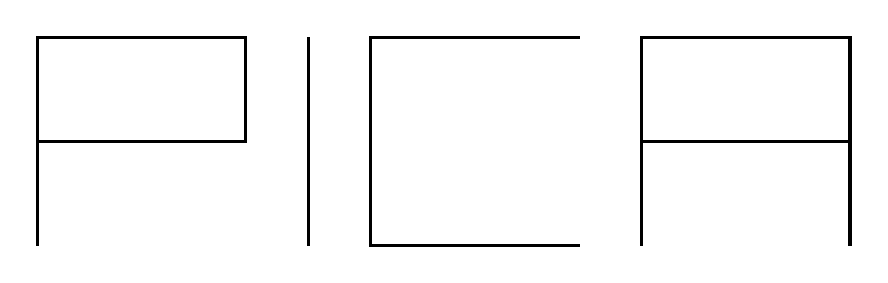
\includegraphics[width=0.9\linewidth]{turtleMPica}
\end{chapterfigure}

\hidden{| caro |
caro := robot new.
"letter P"
caro west; jump: 30 ;jump: 100; north.
caro go: 100; east; go: 100; south; go: 50.
caro west; go: 100; south ; jump: 50 ; east.
caro jump: 130.
"letter I"
caro north; go: 100; south; jump: 100; east; jump: 30.
"letter C" 
caro jump: 100 ; north;  jump: 100 ; west ; go: 100; 
south; go: 100; east; go: 100; jump: 30.
"letter A"
caro north.
caro go: 100.
caro east.
caro go: 100.
caro south.
caro go: 100.
caro north.
caro go: 50.
caro west.
caro go: 100.
}

In this chapter we describe the creation of robots, and the different types of movements that robots know. We propose you some simple experiments to practice what you learned in the previous chapters. We also present how robots may change direction in an absolute manner.  


\section{Creating Robots}
In the previous chapter we mentioned that we created \emph{a} robot, not \emph{the} robot. Indeed, we can create as many robots as we want. Here is a new script \ref{scr:geminiScript} that creates two robots \ct{\caro} and \ct{daly}.

\begin{scriptwithouttitle} \label{scr:geminiScript}
| \caro daly |
\caro := Bot new.
daly := Bot new.
\caro color: Color yellow.
daly jump: 100.
\end{scriptwithouttitle}

The second line creates a robot named \caro as in \scriptref{scr:firstScript}. The third line creates a new robot that we refer to using the variable \ct{daly}. Both robots are created at the same location. In line four, we ask \caro to change its color so that we can distinguish the two robots.



 \st \index{object} is an object-oriented programming language. This means that we create objects and interact with them, or that objects can create other objects and communicate with them.  Moreover, in \st, there are special objects, called  \index{class}\emph{classes}, which are used to create objects. Sending the message \ct{new}\index{\ct{new}} to classes creates an object described by its class. Sending the message \ct{new} to the \ct{Bot} class creates a robot.

To understand what  classes are imagine that a class is a factory. A factory of tin boxes creates many boxes of the same size and shape. After being created, some boxes can be filled, others can be crushed. When one box is crushed, the other boxes are not crushed. The same thing happens with object created inside \sq. In our case, \caro did not move, but \ct{daly} did. You can think of a class as a factory able to produce unlimited supplies of objects of the same type. Once produced, each object exist
independently of the other. 

Class names always begin with an uppercase letter. That's why the
name of the robot class is \ct{Bot} with an uppercase ``B''.
\ct{Color} is also a class producing color objects but we should use a color name
to specify the color we want to obtain. For example, \ct{Color yellow} creates the color yellow.

\largecadre{A class is a factory of objects. Sending the message \ct{new} to a class creates an object of this class.  Class names always start with an uppercase letter. Here \ct{Bot} is the factory creating new robots and \ct{Color} the one for colors.

\begin{nalltt}
Bot new color: Color blue
\end{nalltt}}




\section{Drawing Line Segments}

Asking a robot to draw a line is rather simple as we already saw in the previous chapter. The message \ct{go: 100} asks a robot to move ahead 100 pixels and it leaves a trace during its move. However, even if you were an expert Chinese or Japanese caligrapher, you need to lift the brush from time to time when you drawing. For this purpose a robot knows how to jump, \ie moving forward without leaving a trace. A robot understands the message \ct{jump:}, the argument is the same as with \go, it is a distance in number of pixels. Here is a script which draws two segments. Note that we are hiding the robots from the illustration using the message \ct{beInvisible} so that you can get clearer pictures.

\begin{scriptfig}{turtleMTwoLines}{Two lines}\label{scr:twoLines}
| \caro | 
\caro := Bot new.
\caro go: 30.
\caro jump: 30.
\caro go: 30.
\end{scriptfig}

\begin{exonofig}
Experiment by changing the values in the previous script. 
\end{exonofig}

\begin{exofigwithsize}[0.5]{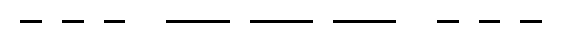
\includegraphics[width=6cm]{turtleMSosLines}}\label{exo:sosLines} 
Generate a script able to draw an SOS message using Morse code.  In
Morse, an "S" is represented by 3 short lines and an "O" is
represented by three long lines as shown by figure on the right.
\end{exofigwithsize}



\section{Changing Directions}
A robot can orient itself along the eight directions as shown by Figure~\ref{fig:roseDesVents}. These directions are like those of a map: east is pointing to the right, west to the left, north up, and south down. To make a robot pointing in a given direction just send it a message with the name of the direction.  So, to ask \caro to face south, one simply types \ct{\caro south}. 

Robots understand  the following messages: \ct{east}, \ct{north}, \ct{northEast}, \ct{northWest}, \ct{south}, \ct{southEast}, \ct{southWest} and \ct{west}. Note that in the next chapter we shall show you how to make a robot turns in a relative manner and from any angle. 

\begin{figure}
\center{\includegraphics[width=10cm]{roseDesVents}}
\caption{The default absolute directions to which a robot can point to.\label{fig:roseDesVents}}
\end{figure}


The script~\ref{scr:mappingrobot} illustrates simply the basic four directions with four different robots. In this script, we use four different robots. Each of them, except
\caro, is oriented toward a different direction before moving. Now we can use the orientation methods to make more complex drawings. As a first exercise draw  a square of 50 pixels size. Then draw another square of 250 pixels.  

\begin{scriptwithtitle}{A gaggle of robots}\label{scr:mappingrobot}
| \caro daly klee sisl |
\caro := Bot new.
\caro color: Color green.
\caro go: 100.
daly := Bot new.
daly north.
daly color: Color yellow.
daly go: 100.
klee := Bot new.
klee west.
klee color: Color red.
klee go: 100.
sisl := Bot new.
sisl south.
sisl go: 100.
\end{scriptwithtitle}


\begin{exofig}{turtleMSmallStairs}
Hopefully we are not limited to squares. One can do a wide range of geometrical figures. For example, here is a drawing of a small stairs. Define the script that reproduces it.
\end{exofig}

%\includegraphics[width=4cm]{robotMSquare}

%Try to define such a script before reading the following one: 

%\begin{scriptfigwithsize}[0.4]{}{A first square}\label{scr:firstSquare}
%| caro |
%caro := robot new.
%caro go: 100.
%caro north.
%caro go: 100.
%caro west.
%caro go: 100.
%caro south.
%caro go: 100
%\end{scriptfigwithsize}


%\begin{scriptfig}{robotMSmallStairs}{Small stairs}\label{scr:smallStairs}
%| caro |
%caro := robot new.
%caro north.
%caro go: 25.
%caro east.
%caro go: 25.
%caro north.
%caro go: 25.
%caro east.
%caro go: 25.
%caro north.
%caro go: 25.
%caro east.
%caro go: 25.
%caro north.
%caro go: 25.
%caro east.
%caro go: 25.
%caro south.
%caro go: 100.
%caro west.
%caro go: 100.
%\end{scriptfig}



\begin{exofig}{turtleMSaqqarah} \label{exo:saqqarah}
Now, we are ready to draw a schematic side view of the pyramid of
Saqqarah, built in 2500BC by Imhotep, the first known architect.
Generate a script able to draw a side view of the pyramid of
Saqqarah. This pyramid has four terrasses and its top is twice as
large than the terrasses as shown in the drawing on the right.
\end{exofig}

\begin{exofigwithtitle}{turtleMArtNouveau}{Pattern} \label{exo:artnouveau}
Draw the picture shown on the right.
\end{exofigwithtitle}

\hidden{
|caro|
caro := robot new.
caro go: 100.
caro turn: 90.
caro go: 100.
caro turn: 90.
caro go: 50.
caro turn: 90.
caro go: 50.
caro turn: 90.
caro go: 100.
caro turn: 90.
caro go: 25.
caro turn: 90.
caro go: 25.
caro turn: 90.
caro go: 50}


\section{The ABC of Drawing}\label{sec:abcDraw} 
Even though the control of the direction of the line segments is
somewhat limited, we can even start to program \caro to
write letters. The script~\ref{scr:letterA} draws an "A".

\begin{scriptfigwithsize}[0.4]{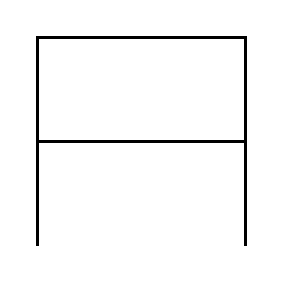
\includegraphics[width=5cm]{turtleMLetterA}}{The letter A}\label{scr:letterA}
| \caro |
\caro := Bot new.
\caro north.
\caro go: 100.
\caro east.
\caro go: 100.
\caro south.
\caro go: 100.
\caro north.
\caro go: 50.
\caro west.
\caro go: 100
\end{scriptfigwithsize}


Drawing a letter "C" is no more difficult. We can 
write a script to write "pica". 

%Here it is:

%\begin{scriptfig}[.35]{robotMBeginCaro}{The beginning of \caro}\label{scr:beginCaro}
%| caro |
%caro := robot new.
%caro west.
%caro jump: 30.
%caro go: 100.
%caro north.
%caro go: 100.
%caro east.
%caro go: 100.
%caro south.
%caro jump: 100.
%caro east.
%caro jump: 30.
%caro north.
%caro go: 100.
%caro east.
%caro go: 100.
%caro south.
%caro go: 100.
%caro north.
%caro go: 50.
%caro west.
%caro go: 100.
%\end{scriptfig}


\begin{exonofig}\label{exo:carosName} 
Draw the name of \caro. Note that as we do not want to have a line between the "C" and the "A" you should use \jump.  
\end{exonofig}

\paragraph{A Remark.}
Some purists  may think that the script~\ref{scr:letterA} could be improved. Indeed, the bottom half of  the left bar of the "A" is drawn twice since the robot is going twice
over this segment --- once going south, once going north. 
Knowing how to write the best program is a difficult question, lot of issues like the speed, the readibility of the code have to be answered and depending of the language, the methods used,..., so there is no simple answer. However, if you ask yourself such a question chose the simplest one.  Then if you have problem after because you program is too slow you can always speed it up.

\section{Controlling Robot Visibility}
We can control whether the robot should be displayed or not using the message  \ct{beInvisible} and \ct{beVisible}. \ct{beInvisible}\index{beInvisible} hides the receiver. A hidden robot acts exactly as a normal one but it just does not show where it is. Be careful attention because the method \ct{hide} already exists but it is defined by \sq and can damage the robot environment. \ct{beVisible}\index{beVisible} shows the receiving robot. A newly created robot is showing itself by default. 


\summa


\begin{table}[h]
  \centering
\begin{tabular}{| p{4cm} | p{5cm} | l |} \hline
  % after \\ : \hline or \cline{col1-col2} \cline{col3-col4} ...
  \hfil Expressions Messages & \hfil Description & \hfil Example \\[1ex] \hline
  \ct{Bot new} & Create a computer robot & \ct{pica := Bot new} \\ \hline
  \ct{| x y |} & Declare variables used in the script & \ct{| pica |} \\ \hline
  \ct{jump: anInteger}  & Ask a robot to move forward by a given number of pixels without leaving a trace & \ct{pica jump: 10} \\ \hline
  \ct{go: anInteger} & Ask a robot to move forward by a given number of pixels while leaving a trace & \ct{pica go: 10} \\ \hline
\ct{beInvisible}& Ask a robot to be invisible& pica beInvisible\\ \hline
\ct{beVisible}& Ask a robot to be visible& pica beVisilble\\ \hline
\ct{east}, \ct{north}, \ct{northEast}, \ct{northWest}, \ct{south}, \ct{southEast}, \ct{southWest} and \ct{west}& Ask a robot to point to the corresponding direction& \ct{pica north} \\ \hline
  \ct{Color }{\emph xxx} &Create a color& \ct{Color blue} \\ \hline
  \ct{color: aColor}&Ask a robot to change its color.& \ct{pica color: Color red} \\   \hline
\end{tabular}

\end{table}

\ifx\wholebook\relax\else\end{document}\fi
%O+I => final
%4 Released
%O+I
% Dominic feedback => final
% 23 Dec 2004

\ifx\wholebook\relax\else
\input{../Common.tex}
\input{../macroes.tex}
\begin{document}
\fi


\chapter{Directions and Angles}\label{ch:relativeTurn}


\begin{chapterfigure}
\hfil 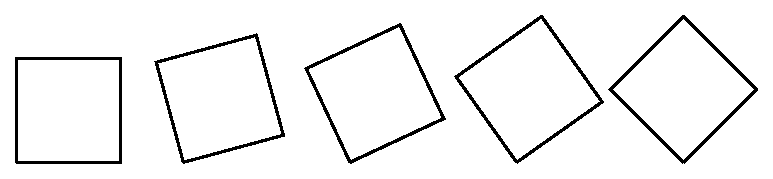
\includegraphics[width=0.9\linewidth]{ChTurntitlePicture}\hfil
\end{chapterfigure}


\hidden{
finalVersion
titlePicture
	
	| caro |
	caro := Turtle new.
	caro go: 50.
	caro turnLeft: 90.
	caro go: 50.
	caro turnLeft: 90.
	caro go: 50.
	caro turnLeft: 90.
	caro go: 50.
	caro turnLeft: 90.
	caro jump: 80.
	caro turnLeft: 15.
	caro go: 50.
	caro turnLeft: 90.
	caro go: 50.
	caro turnLeft: 90.
	caro go: 50.
	caro turnLeft: 90.
	caro go: 50.
	caro turnLeft: 90.
	caro east.
	caro jump: 80.
	caro turnLeft: 25.
	caro go: 50.
	caro turnLeft: 90.
	caro go: 50.
	caro turnLeft: 90.
	caro go: 50.
	caro turnLeft: 90.
	caro go: 50.
	caro turnLeft: 90.
	caro east.
	caro jump: 80.
	caro turnLeft: 35.
	caro go: 50.
	caro turnLeft: 90.
	caro go: 50.
	caro turnLeft: 90.
	caro go: 50.
	caro turnLeft: 90.
	caro go: 50.
	caro turnLeft: 90.
	caro east.
	caro jump: 80.
	caro turnLeft: 45.
	caro go: 50.
	caro turnLeft: 90.
	caro go: 50.
	caro turnLeft: 90.
	caro go: 50.
	caro turnLeft: 90.
	caro go: 50.
	caro turnLeft: 90
}

By now you should be getting tired of drawing figures only in \emph{fixed} directions. In this chapter you shall learn how to change the direction in  which a robot moves and draws a line in \emph{any} direction and in relative manner. For this purpose, we present the mathematical concept of angle to indicate to a robot how far it should turn. However, if you understand clearly what an angle is and how to measure angles in degrees, you may skip Section~\ref{sec:angles} and proceed readily with the examples and experiences of Section~\ref{sec:angleExperiments}. 

We start by presenting the elementary messages that robots understand to change their direction. Note that we are hiding the robots from the illustrations using the message \ct{beInvisible} so that you can get clearer pictures. 


\section{Right or Left?}\label{rightleft}
In the previous chapter, you learned that a robot could face different directions using the messages \ct{east}, \ct{north}, \ct{northEast}, \ct{northWest}, \ct{south}, \ct{southEast}, \ct{southWest} and \ct{west}. However, with these messages you can not change the direction of your robot from a given angle such as 15 degrees. In addition, you cannot say that you want for example turn a robot of a quarter of a turn from the current direction. 

To orientate a robot along any direction you should use the two methods
\turnLeft and \turnRight which ask a robot to turn to the left or the right. As the colon at the end of the names indicates, both methods are expecting an argument. This argument is the angle between the heading of the robot before and after issuing the message. This angle is given in degrees. For example the expression \ct{\caro turnLeft: 15} asks \caro to turn on the left fifteen degrees from its current direction and \ct{\caro turnRight: 30} turns on the right 30 degrees from its current direction. Figure~\ref{fig:turnLeftBoth} illustrates the effect of the messages \ct{turnLeft:} and \ct{turnRight:} first when a robot is pointing to the east and second when a robot is pointing to another direction.  


Now you should practice but remember that when a new robot is created, it always points to the east or the right of the screen. 

\begin{figure}
\begin{center}\includegraphics[width=16cm]{turnLeftBoth}
\caption{Left: turning left or right from the east position. Right: turning left of right from another position. \label{fig:turnLeftBoth}}
\end{center}
\end{figure}


\begin{exonofig} 
Read the following scripts Problem One (\scriptref{scr:proone}) and Problem Two (\scriptref{scr:protwo}) and try to guess what the created robot will do. Then experiment with the scripts: Change the angle values for example to determine what is the angle so that the robot turns a quarter, an half of a complete turn or a complete turn. If you have problem with the notion of angle read carefully the Section~\ref{sec:angles} before continuing.
\end{exonofig}


\begin{ncscript}{Problem One}\label{scr:proone}
| \caro |
\caro :=  \Turtle new. 
\caro go: 100.
\caro turnLeft: 45.
\caro go: 50.
\caro turnLeft: 45.
\caro go: 100\end{ncscript}

\begin{ncscript}{Problem Two}\label{scr:protwo}
| \caro |
\caro := \Turtle new. 
\caro go: 100.
\caro turnRight: 60.
\caro go: 100.
\caro turnLeft: 60.
\caro go: 100\end{ncscript}

\paragraph{About Mathematical Conventions.} In mathematics, there exist some conventions for the rotations: a rotation with a negative angle is clockwise and with a positive angle inverse clockwise. In this book, you can  also follow the mathematical conventions, using the message \ct{turn:}. Hence, the message \ct{turnLeft: anAngle} is equal to the message \ct{turn: anAngle} while, the message \ct{turnRight: anAngle} is equal to \ct{turn: - anAngle} that is the angle negated as shown by the Figure~\ref{fig:turnLeftWithMathematicalEq}. 


\begin{figure}
\begin{center}\includegraphics[width=8cm]{turnLeftWithMathematicalEq}
\caption{Some angles starting from the east directions.\label{fig:turnLeftWithMathematicalEq}}
\end{center}
\end{figure}




\section{Absolute versus Relative Orientation}
Now you should feel confident that you can ask a robot to execute any
drawing made with lines of any sort. Before going further, have you
understood the difference between orienting a robot using the
methods \north, \south, \east, and \west and using the methods \turnLeft and \turnRight?
Figure~\ref{fig:roserelative} shows some angles which are measured starting from the east direction. 

To explain the difference we ask you to complete the following experiments \ref{exo:relativeSquare}, \ref{expturntt} and \ref{expturntttwo}.

\begin{exofigwithsizeandtitle}[0.4]{\includegraphics[width=4cm]{ChTurnfirstSquare}}{A Relative Square} \label{exo:relativeSquare} 

\hidden{%%firstSquare
| caro |
	caro := Turtle new.
	caro go: 100.
	caro turnLeft: 90.
	caro go: 100.
	caro turnLeft: 90.
	caro go: 100.
	caro turnLeft: 90.
	caro go: 100.
	caro turnLeft: 90.}

Define a script drawing a square using the methods \turnLeft or \turnRight.
\end{exofigwithsizeandtitle}

\begin{exonofig}\label{expturntt}
Now, add the following line: \ct{\caro turnLeft: 33.}  before the first
line containing a \go message in the script you just defined.  As you can see one still obtains a square, but it is tilted. 
\end{exonofig}

\begin{exonofig}\label{expturntttwo}
Finally type the \scriptref{scr:badSquare} that draws a square but only using the methods \north, \south, \east and \west that we presented in the previous chapter. 
\end{exonofig}

\begin{scriptfigwithsize}{\includegraphics[width=4cm]{ChTurnbadSquare}}{A Broken Square} \label{scr:badSquare}
| \caro |
\caro := \Turtle new.
\textit{\caro \turnLeft 33.}
\caro go: 100.
\caro north.
\caro go: 100.
\caro west.
\caro go: 100.
\caro south.
\caro go: 100.
\end{scriptfigwithsize}

Do you still obtain a square? No! The first side drawn by the robot
is slanted whereas the other sides are either horizontal or
vertical. What these two scripts \scriptref{scr:badSquare} and
\scriptref{exo:relativeSquare} show you is the difference between
\emph{relative} and \emph{absolute} direction changes.

\begin{itemize}
\item The methods \north, \south, \east and \west change direction in an  \emph{absolute} manner.  The direction to which the robot will point does \emph{not} depend on the current direction in which it is pointing.

\item The methods \turnLeft and \turnRight change direction in a \emph{relative} manner. The direction to which the robot will point \emph{depends} on its current direction.
\end{itemize}

Figure~\ref{fig:roserelative} shows the equivalence between relative moves starting with a robot pointing to the east and absolute moves. As you know know, this equivalence is not correct if the robot is pointing to any other direction than the east. It is worth to note that turning 180 degrees makes the robot pointing in the opposite direction which is often used in the scripts.

\begin{figure}[h]
\begin{center}\includegraphics[width=8cm]{roseDesVentsRelatifToo}
\caption{Comparing absolutes and relative angles starting from the east direction.\label{fig:roserelative}}
\end{center}
\end{figure}


\section{The Right Angle of Things}\label{sec:angles}
As you should know by now, a newly created robot is pointing east,
that is, toward the right hand side of the screen. If we ask this
robot to turn left by 90 degrees, it will end up heading north. If we
ask it to turn right by 90 degrees, it will end up heading south. Here
is a script (\ref{scr:angleSearch}) illustrating what a turn left by 45 degrees is doing. To help you following it we added the starting position of the robot.

\begin{scriptfig}{ChTurnangleSearchAnnotated}{The meaning of angles} \label{scr:angleSearch}
| \caro |
\caro := \Turtle new.
\caro west.
\caro go: 100.
\caro east.
\caro turnLeft: 45.
\caro go: 100.
\end{scriptfig}

The first part of script~\ref{scr:angleSearch}, up to the line \ct{\caro east}, draws an
horizontal line to indicate the eastern direction. The last part draws
the line in the direction 45 degrees left of the east direction. You
can vary the value of the angle to see what other values
represent. Try the values 60, 120, 180, 240, 360, and 420. In
particular, note that a turn by 180 degrees amounts to going back on the
previous direction.

Do you see any difference between 60 and 420? No. Any two angle values
whose difference is 360 or any multiple thereof are equivalent. Try an
angle value of  1860 ($1860 = 60  + 360 \times 5$). The  result is the
same as  that with angle values  60 and 420.  360  degrees represents a
single turn. As  far as orienting oneself, it  does not matter whether
you add one  or more full turns to the orientation.  Keep this in mind
when dealing with angles.

Now, let us try the method \turnRight. Script~\ref{scr:angleSearch2} draw two needles of and old watch and a reference line. It uses two robots, that you can use to investigate the correspondence between a left or a right turn.  We added comments surrounded by \ct{"} and use different font effects to help you to identify the different parts in the script. Note that you do not have to type these comments as they do not get executed. 


%%DoubleTurtles@@
\begin{scriptfig}{twoAnglesAnnotated}{The meaning of angles (2)} \label{scr:angleSearch2}
| \caro daly |
\caro := \Turtle new.
\emph{\caro jump: 200.}                        "drawing the reference line"
\emph{\caro turnLeft: 180.
\caro go: 200.
\caro turnLeft: 180.}
\caro color: Color blue.
\caro turnLeft: 45.                 "drawing the long needle"
\caro go: 150.
daly := \Turtle new.
daly color: Color red.
\textbf{daly turnRight: 45.}              "drawing the short needle"
\textbf{daly go: 100.}                             
\end{scriptfig}

In script~\ref{scr:angleSearch2}, the code in italic draws the reference line --- that is the line representing the direction of the robot before issuing a turn method
--- using the fact that a turn by 180 degrees amounts to go back in the
opposite direction. The reference line is also the  longest lines drawn. Thus, 
the reference line will still be visible if the lines drawn by the robots fall on top of it. 
Then in normal font is the code that draws the longest needle (using \caro) and in bold the code drawing the short needle using the variable \ct{pica}. This is similar to the needles of an old time clock.

%The reference line, that is the line representing the initial direction, is drawn by \caro, but it is common to both robots. Indeed, we have seen that all robots are created equal.  In particular, they both point to the eastern direction initially.

\begin{exonofig} Repeat the same series of angle values for both
 robots, that is, change the angle value for the two turn methods.
Then, compare the effect of the method \turnLeft\ \ct{60} (for
\caro) and \turnRight\ \ct{300} (for {\ct{daly}}). You can see
that turning left by 60 degrees is the same as turning right 300
degrees because the sum of the two values is 360 degrees, that is a
full turn.
\end{exonofig}

\begin{exonofig} 
Now let us see what happens when turning from another direction.  Here
is the same script as \scriptref{scr:angleSearch} but showing the
effect of turning from the north direction.

%%DoubleTurtles@@
\begin{scriptfig}{threeAngles}{The meaning of angles (3)} 
\label{scr:angleSearch3}
| \caro marge |
\caro := \Turtle new.
\textbf{\caro north.}
\caro jump: 200.
\caro turnLeft: 180.
\caro go: 200.
\caro turnLeft: 180.
\caro color: Color blue.
\caro turnLeft: 45.
\caro go: 150.
daly := \Turtle new.
daly north.
daly color: Color red.
daly turnRight: 45.
daly go: 100.
\end{scriptfig}
\end{exonofig} 

\begin{exonofig}
Continue to experiment with the \scriptref{scr:angleSearch3} by changing
the direction of reference. For the comparison to be meaningful, you
have also to orient \ct{daly} to the same direction than \caro after
creating it. Try any angle values you like and try to predict what the
resulting drawing will look like before executing the script. Continue
experimenting with that script until your predictions are good.
\end{exonofig}

Note that it is important that you can always predict what is going to happen
before executing a script because a computer blindly executes statements, even the silliest ones.


\section{A Robot Clock}
We have mentioned that the lines drawn in the \scriptref{scr:angleSearch3}
were akin to that of an old time watch. The analogy is more than
real. The notion of degrees is strongly correlated to that of hours,
because the ancient peoples discovered the notion of time by measuring the
angle of the sun (or some star) respective to a direction of reference.
However with the previous code you could draw a clock indicating an hour that was not true, that is the small needle pointing to the north and the long one to the south. 

Now you will study the relationship between the small needle and the long one to represent a \emph{real} hour: if the long needle is pointing on the south then the short one should be half of the hour distance between two numbers. Modify \scriptref{scr:angleSearch3} and proceed as follows:

\begin{enumerate}
\item Keep the direction of reference to the north (this is how
\scriptref{scr:angleSearch3} is written). The reference line
indicates noon.
  
\item Use the method \turnRight for both robots. A turn
 to the right is what the needles of an old time clock are doing.
  
\item You can ask \caro to draw the minute needle by
multiplying the number of the minutes you want to indicate by 6.
For example, 20 after the hour is shown with the message 
\ct{turnRight: 120} ($120 = 6 \times 20$).
  
\item You can ask \ct{marge} to draw the hour needle by
multiplying the number of the hours you want to indicate by 30.
For example, 2 o'clock is shown with the message
\ct{turnRight: 60} ($60 = 30 \times 2$).
\end{enumerate}

Try to indicate a few hours of your choice with that script.

\section{Simple Drawings}\label{sec:angleExperiments} 
To begin with, here is a script drawing a triangle:

\begin{scriptfigwithsize}[0.4]{\includegraphics[width=4cm]{ChTurnfirstTriangle}}{A triangle} \label{scr:firstTriangle}
| \caro |
\caro := \Turtle new.
\caro go: 100.
\caro turnLeft: 120.
\caro go: 100.
\caro turnLeft: 120.
\caro go: 100
\end{scriptfigwithsize}

Now, you are ready to draw a house.

\begin{exofigwithsize}{\includegraphics[width=2cm]{ChTurnbabyHouse}}\label{exo:babyHouse} 
Draw a house as shown on the right. Try to draw houses of different shapes.
\end{exofigwithsize}

\hidden{%%babyHouse
	| caro |
	caro := Turtle new.
	caro go: 100.
	caro turnLeft: 90.
	caro go: 100.
	caro turnLeft: 90.
	caro go: 100.
	caro turnLeft: 90.
	caro go: 100.
	caro turnLeft: 180.
	caro jump: 100.
	caro turnRight: 90.
	caro jump: 100. 
	caro turnLeft: 120.
	caro go: 100.
	caro turnLeft: 120.
	caro go: 100}



\section{Regular polygons} \label{sec:firstPolygons} 
A regular polygon is a figure made with line segments of the same
length. An equilateral triangle is a regular polygon with 3 sides. A
square is a regular polygon with 4 sides.  For example, the
\scriptref{scr:firstTriangle} that draws an equilateral triangle,
whose side length is 100 pixels, is obtained by asking \caro to go
forward a given distance and to turn 120 degrees left or right, the two
commands repeated 3 times. Note that there is a relationship between the 
number of sides and the angle: the angle is equal to 360 degrees divided 
by the number of sides. 

Program a robot to draw a regular polygon with any number of
sides by asking it to go for some length and then turn left or right
by 360 degrees divided by the number of sides; this sequence must be
repeated as many times as there are sides.




\begin{exofig}{ChTurnpentagon} \label{exo:pentagon}
Try to draw a pentagon, that is a regular polygon with five sides
of 100 pixel length.
\end{exofig}

\hidden{	| caro |
	caro := Turtle new.
	caro go: 100.
	caro turnLeft: 72.
	caro go: 100.
	caro turnLeft: 72.
	caro go: 100. 
	caro turnLeft: 72.
	caro go: 100.
	caro turnLeft: 72.
	caro go: 100.}

\begin{exofig}{ChTurnhexagon} \label{exo:hexagon}
Try to draw a hexagon, that is a regular polygon with six sides of
100 pixel length.
\end{exofig}

\hidden{%%Hexagon
	| caro |
	caro := Turtle new.
	caro go: 100.
	caro turnLeft: 60.
	caro go: 100.
	caro turnLeft: 60.
	caro go: 100. 
	caro turnLeft: 60.
	caro go: 100.
	caro turnLeft: 60.
	caro go: 100.
	caro turnLeft: 60.
	caro go: 100.}

Maybe, you are just curious to see how far you can go. Using the
cut and paste facility of the \tw, you can
actually generate a regular polygon with a large number of sides.
If you are in the mood, go on increasing the number of sides. However
in the next chapter we will show you how this can be solved. 

\ 


\begin{exofigwithsize}{\includegraphics[width=4cm]{ChTurnc3pace}}\label{exo:pace}
Draw the symbol shows by the figure on the  right.
\end{exofigwithsize}



\hidden{c3pace
| caro |
	caro := Turtle new.
	caro go: 100.
	caro turnLeft: 180.
	caro jump: 100.

	caro turnLeft: 60.
	caro go: 100. 
	caro turnLeft: 180.
	caro jump: 100. 

	caro turnLeft: 60.
	caro go: 100. 
}


\summa
\begin{enumerate}
\item A robot can be oriented \emph{relatively} to its \emph{current}
  direction using the methods \turnLeft and \turnRight.
\item The parameter given to the methods  \turnLeft and
\turnRight is given in degrees.
  \item Turning 360 degrees corresponds to a full turn.
	\item Turning  180 degrees corresponds to an half turn.
  \item Angles values whose difference is a multiple of 360 degrees
  are equivalent.
\end{enumerate}

Here is the list of the methods which you have learned in this chapter.
\begin{table}[h]
  \centering
  \begin{tabular}{| l | p{5cm} | l |} \hline
  % after \\ : \hline or \cline{col1-col2} \cline{col3-col4} ...
  \hfil Method & \hfil Description & \hfil Example \\[1ex] \hline
  \turnLeft & Ask the robot to change its direction to a number of given degrees to the left & \ct{\caro turnLeft: 30} \\ \hline
   \turnRight & Ask the robot to change its direction to a number of given degrees to the right & \ct{\caro turnRight: 30} \\
  \hline
   \ct{turn:} & Ask the robot to change its direction to a number of given degrees following the mathematical convention:  to the left is the number is positive and to the right if it is negative & \ct{\caro turn: -30} \\ \hline

\ct{beInvisible}& Hide the receiver & \ct{\caro beInvisible} \\
  \hline
\ct{beVisible}&Show the receiver& \ct{\caro beVisible} \\
  \hline

\end{tabular}
\end{table}


\ifx\wholebook\relax\else\end{document}\fi
%O+I + Dominic => final

%5 Released
% O+I 
% TD: \item Using keyboard shortcuts. Select a piece of text, then press command-d on mac and alt-d @@to verify@@)

\ifx\wholebook\relax\else
\input{../Common.tex}
\input{../macroes.tex}
\begin{document}
\fi

%%%%%%%%%%%%%%%%%%%%%%%%%%%%%%%%%%%%%%%%%%%
\chapter{Pica's Environment}\label{cha:caroTour}

In this chapter, I will present the environment, show you how you can get the tools, save your scripts. I will also we return to the notion of messages and show that you can ask the environment to execute a message but also to print the \emph{result} of the message execution. 


\section{Looking at the Main Menu}
When you click on the background you get the main menu of the environment as shown by Figure~\ref{fig:allMenu}. 


\begin{figure}[h]
\begin{center}
\includegraphics[width=8cm]{allMenu}
\caption{Menu options of the environment.\label{fig:allMenu}}
\end{center}
\end{figure}

If you want to know what each menu item does, simply let the mouse pointer on it for one second, a balloon should pop up describing the item. The main menu gives access to five main groups of functionalities: access to tools, screen capture, access to some robot behavior, appearance,  and saving the environment. The submenus are grouped as follows: 

\begin{itemize}
\item[open...] The menu \button{open...} groups several tools such as the robot code browser, the \tw, a file browser and other tools that I will present when needed
\item [BotInc actions] The menu \button{BotInc actions} groups several actions such as indicating the version of the environment, clear all the robots and their traces, but also some actions to reinstall the environment if needed: reinstall default preferences set back the default preferences that you may have modified using the following menu. 
\item [appearance] The menu \button{appearance...} groups actions related to change the appearance of the environment such as the fonts used, the full screen mode, the color of the background.
\end{itemize}


\paragraph{Getting a \tw.}
It may happen that you close the default \tw. This is not a problem as you can get a new one easily from the dark blue flap as shown by Figure~\ref{fig:caroflaps} or from the main menu as shown before. To install a new \tw in the working flap, open the working flap (bottom flap) and drop the bot workspace from the blue flap into the bottom flap. 

\begin{figure}
\begin{center}
\includegraphics[width=7cm]{smallcaroflap}\hfill\includegraphics[width=7cm]{FullTurtleWorkspace}
\caption{Getting a new \tw from the flaps. \label{fig:caroflaps}}
\end{center}
\end{figure}

The dark blue flap contains other tools that we are going to use in the future. Basically, the second tool is a code browser that you will use when you will define new robot methods. 


\section{Interacting with \sq}
\sq interaction is based on the assumption that you have a three button mouse. Each button is associated with a logical set of operations. The left button is for pointing and selecting, the middle button is for window manipulation (bringing a window in front, moving it), and the right button for bring context sensitive menu and handles which are small colored and round buttons floating around graphical elements (as shown in Figure~\ref{fig:rohals}). The handles are useful as they allow you to interact directly with the robot. I will present them in detail in the next chapter.  

\begin{figure}[h]
\begin{center}
\includegraphics[width=8cm]{picaAllHaloAnnotated}
\caption{Right-clicking on a robot brings its handles.\label{fig:rohals}}
\end{center}
\end{figure}


Depending on your machine, you will need to click with different mouse button and key combinations as explained by the following table: 

\begin{center}
\begin{tabular}{|| p{2.5cm} | p{3cm} | p{3cm} | p{3cm} ||} \hline \hline
Button:           &   Left       &    Center       &  Right \\ \hline \hline
Kind of Actions:  &  Pointing, selecting     & Context    sensitive menu  &   Bringing halos \\ \hline
Windows 2-Button  Equivalent&   Left-Click    & Alt-Left    &   Right Click \\ \hline
Mac 1 Button  Equivalent&  Click      &    Option-click &  Cmd-Click \\ \hline 
\hline
\end{tabular}
\end{center}


\section{Using \tw to Save a Script}
The \tw has 5 buttons and also a menu that allows you to save scripts.
The button \textbf{Do It All} executes the entire script that the workspace contains.
The button \textbf{Do It} executes the part of the script that is currently selected in  the workspace. The button \textbf{Clear Trails} clears only the robot trails without removing the robots themselves. The button \textbf{Clear Robots} removes only the robots without cleaning their trails. The button \textbf{Clear All} removes all the robots and their trails.

Once you have written a script you may wish to save to a file  for future uses. The \tw provides a way of saving and loading files via its menu. 

\begin{figure}[h]
\includegraphics[width=7cm]{saveContents}
\includegraphics[width=4cm]{enteringFileName}\includegraphics[width=4cm]{overwrite}
\caption{\tw menu options.  Middle: Specifying the name of the file in which the script is saved. Right: When the file already exist you can overwrite it or rename it.\label{fig:turtleMenu}\label{fig:enteringFileName}}
\end{figure}

Click on the contents of the workspace to bring up its associated menu as shown in Figure~\ref{fig:turtleMenu}. The menu item \menu{save contents} will save the complete contents of the workspace into a file. Selecting this menu item brings up a dialog box as shown in Figure ~\ref{fig:enteringFileName}. Note that the system checks whether a file with the same name already exists or not. If such a file already exists, the system asks you if the file should be overwritten or to provide another name as shown in Figure ~\ref{fig:enteringFileName}.


\section{Loading a Script}
To load a script, you have to use a \index{file list} \fl, a tool that allows you to select and load different files into \sq. You can obtain a file list by selecting the menu item \button{open...} and \button{file list} from the main menu.  A \fl is composed of several panes. The top left pane allows you to navigate the volumes and folders, each time you select an item in this pane the top right pane is updated. It shows all the files contained in the folder you selected in the left pane. When you select a file in the right pane, the bottom pane automatically shows its contents. Figure~\ref{fig:filelistOpen} shows we are in  the folder \ct{Bot testing} in  which  the file \ct{square.text} is selected. 


%\begin{figure}
%\begin{center}
%\includegraphics[width=6cm]{fileListInFlap}\caption{The FileList thumbnail available in the Advanced Flap. \label{fig:fileListInFlap}}\end{center}
%\end{figure}


\begin{figure}[h]\begin{center}
\includegraphics[width=12cm]{filelistOpenAnnotated}
\caption{The \fl opened on the script named \ct{square.text}.\label{fig:filelistOpen}}\end{center}
\end{figure}

To load a script you simply have to copy  the contents of the bottom pane using the menu item (\menu{copy}) and paste  (\menu{paste}) it into the \tw as you would do with any texteditor.   





%\begin{figure}
%\includegraphics{copyFromFileList}
%\end{figure}




\section{Capturing a Drawing}
To keep a trace of your drawings you can use the screen capture of your computer. However, on certain computers you may have problem to get a screen capture. To avoid this problem, the environment proposes a simple screen capture mechanism that works on any computer. Bring the main menu by clicking on the background of the environment. The menu offers two items named: \menu{capture screen} and \menu{capture and save image} as shown by Figure~\ref{screenCapture}. 

The easier way is to use the \menu{capture and save image} menu item. When you select this item \sq shows that it is ready to capture by changing the cursor to be like a corner as shown by Figure~\ref{screenCapture}. Place the cursor and click at the corner of the rectangular region you want to capture, hold down the menu and move the mouse to delimit the region you want. The region is shown in the bottom left corner and \sq prompts you to get the name of the file without extension that it will save.

\begin{figure}[h]
\begin{center}
\includegraphics[width=7cm]{screenCapture} \includegraphics[width=7cm]{positioningScreen}
\caption{Left: Two possibilities to capture and save the capture. Right: The cursor is changed. \sq is ready for the capture. Now click to position one corner of the rectangular region you want to capture.}\label{screenCapture}
\end{center}
\end{figure}


Now you may want to sort and choose the screen captures that you want to keep. For that you can capture a region of the screen using the menu item \menu{capture screen}. In such a case \sq will not prompt you to save the file, but instead it creates a picture on the \sq desktop.  Then you can save it by bringing the handles by right-clicking on it. You should get different handles around the image as shown by Figure~\ref{sketchWithHalo}. Once the halos are there around your image, click on the red handle which brings a menu of actions that you can apply on the image. Select the \menu{export...} item and the format in which the image will be save. \sq will prompt you for the name of the file. Note that you can import in \sq these files by dropping them from the desktop into the \sq desktop. 



\begin{figure}
\begin{center}
\includegraphics[width=4cm]{sketchWithHalo}
\includegraphics[width=9cm]{sketchExportMenu}
\caption{Bring the halos and chose the red halo menu item \menu{export...} to save the image on disk.} \label{sketchWithHalo}
\end{center}
\end{figure}




\section{Message Result}
In \st, objects only communicate by receiving from and sending messages to other objects. Once an object receives a message it executes it and it may return a \index{result} \emph{result}. A result is an object that you get back from a message.
In a similar fashion that for some letters that we receive, we need to perform actions and for others we need to sign an acknowledgment that we effectively received the letter. 

For example sending the message \ct{go: 100} to a robot asks the robot to move 100 pixels in its current direction. But there is no result returned. In certain cases the result of a message execution is important. For example, sending the message \ct{+ 3} to the object \ct{2} returns \ct{5}. Sending the message \ct{color} to a robot returns its current color. The result of a message is important to be able to compose multiple messages. For example, when the expression \ct{(2+ 3) * 10} is executed, the expression \ct{(2 + 3)} returns \ct{5}. This number is then used in another message \ct{* 10} which finally returns \ct{50}.

\cadre{A result is an object that you get from a message. 

\begin{nalltt}
2 + 5 \\
    returns 7\\
pica color\\
    returns its color, a color object
\end{nalltt}}

The \sq environment allows you to \textit{execute messages} without taking care of the message's result, or execute messages \textit{and print the returned message value}. If the difference is not really clear the following example illustrates it. Imagine that you have a small robot that carries items. When you tell him to move, the robot will just move but you will not get anything back. Now if you ask the robot to give you an item, it will execute this order by moving one of its physical elements \textit{and} gives you the item.  This example illustrates the difference between executing a message and executing a message that returns a value. 

\paragraph{Vocabulary Point.} In \sq jargon printing an result means giving an ascii (character-based) format version of the result just after the expression and not on a physical printer. In Figure~\ref{fig:printitMenu} \ct{140} is composed of three characters that represent the number one hundred forty and one hundred fifty is the result returned by the sum of the number fifty and ninety.

\begin{figure}[h]
\includegraphics[width=5cm]{selectingExp}  \includegraphics[width=5cm]{selectMenu}\includegraphics[width=5cm]{resultExpression}
\caption{Left: Selecting the expression \ct{50 + 90}. Middle: Bringing the menu. Right: Executing it and getting the result printed.\label{fig:printitMenu}}
\end{figure}


Now there are three ways of executing a script.
\begin{enumerate}
\item Using the buttons of the \tw editor.  In \charef{cha:firstscript} I show you a simple way to execute your first code by pressing the \button{Do It All} button of the \tw. But to execute a script you can also \emph{select} the text you want to execute with the mouse (the selection goes green) and you press the \button{Do It} of the \tw.

\item Using the menu. Select the part of your script you want to execute as shown by \index{executing} Figure~\ref{fig:doitMenu}, get the menu by pressing  the middle button of your mouse (or press the option key while clicking with the left button), then  chose the \menu{do it (d)} or the \menu{print it (p)} menu item as shown by the Figure~\ref{fig:printitMenu}. 

\item Using keyboard shortcuts. Select a piece of text, then press command-d on mac and alt-d on PC).
\end{enumerate}



\paragraph{Hints.} To automatically select all the text, you can just click at the start of the text (before the first character) or at the end of the text, or on the line after the last expression.  If you want to select a word, you can just double-click anywhere on the word.  If you want to select a line just double-click at the beginning (before the first character) or end (after the last character) of the line.

 
\begin{figure}[h]
\begin{center}
\includegraphics[width=8cm]{doitViaMenu}
\caption{Selecting a piece of a script and executing it explicitly using the menu.\label{fig:doitMenu}}
\end{center}
\end{figure}


\paragraph{Two Examples.}
When you execute the message \ct{\caro color} which asks the robot its color using the \menu{do it (d)} menu item, the message is effectively sent and executed. However, you have the impression that nothing happens. This is because you do not ask the system to take care about the result of the message execution. When you are interested by the result of a message you should use the menu item \menu{print it (p)} as shown by Figure~\ref{fig:colorPrintIt}. This has the effect to execute the piece of code selected \emph{and} print the result returned by the last message composing the code.
Here the message \ct{\Turtle new} is executed, then the message \ct{color} is sent to the newly created robot. The message \ct{color} is executed and the color of the receiving robot is returned and printed as shown by Figure~\ref{fig:resultColorPrintIt}.
 \ct{(TranslucentColor r: 0.0 g: 0.0 b: 1.0 alpha: 0.847)} tells us that the color of the robot is a transparent color composed from the three color component red, green and blue.






\begin{figure}
\centerline{\includegraphics[width=8cm]{colorPrintIt}} 
\caption{Bring the menu and select the menu item \menu{Print it (d)} to execute the selected piece of code \textit{and} print the returned result.\label{fig:colorPrintIt}}
\end{figure}

\begin{figure}
\centerline{\includegraphics[width=8cm]{resultColorPrintIt}} 
\caption{Bring the menu and select the menu item \menu{Print it (d)} to execute the selected piece of code \textit{and} print the returned result.\label{fig:resultColorPrintIt}}
\end{figure}

Let's look at a final example to make sure that you understand when to use  \menu{print it}. When you execute the message \ct{100 + 20} using the menu item \menu{do it (d)}, the message \ct{+ 20} is effectively sent to the object \ct{100} that adds \ct{20}. However you do not see anything. This is normal because in  such a case the execution of the \ct{+} message returns a new number representing the sum but you did not ask \sq to print it. To see it you have to print the result of the message execution using the menu item \button{Print It}. From now  we will use \pr to indicate that we use the \menu{print it} to get the message executed and its result printed as shown in the scripts \ref{scr:doitprint}. Note that we will only use this convention when the result is important. 


\begin{scriptwithtitle}{Printing the result of an expression execution}\label{scr:doitprint}
(100 + 20) * 10
\pr 1200
\end{scriptwithtitle}


\begin{largecadre}{There are two ways of executing an expression: using the \menu{Do It} menu item to execute an expression. Using the   \menu{Print it} menu item to  execute it and print the returned result.}
\end{largecadre}




\summa
\begin{itemize}
\item \emph{To execute an expression}. Select a piece of text representing one or several expression and press the \button{Do It} button or select the menu item
\menu{do it} from the execution menu.

\item A result is an object that you get from a message. For example, \ct{pica color} returns the color of the robot.

\item There are two ways of executing an expression: using the \menu{Do It} menu item to execute an expression. Use the   \menu{Print it} menu item to  execute it and print the returned result.

\end{itemize}


\ifx\wholebook\relax\else\end{document}\fi



%%O+I + Dominic => final
%=> release by Jon => David

%6
% $Author: stef $
% $Date: 2008-04-04 17:14:31 +0200 (Fri, 04 Apr 2008) $
% $Revision: 318 $
%=================================================================
\ifx\wholebook\relax\else
% --------------------------------------------
% Lulu:
    \documentclass[a4paper,10pt,twoside]{book}
    \usepackage[
        papersize={6in,9in},
        hmargin={.75in,.75in},
        vmargin={.75in,1in},
        ignoreheadfoot
    ]{geometry}
    \input{../common.tex}
    \pagestyle{headings}
    \setboolean{lulu}{true}
% --------------------------------------------
% A4:
%   \documentclass[a4paper,11pt,twoside]{book}
%   \input{../common.tex}
%   \usepackage{a4wide}
% --------------------------------------------
    \graphicspath{{figures/} {../figures/}}
    \begin{document}
%   \renewcommand{\nnbb}[2]{} % Disable editorial comments
    \sloppy
\fi

\chapter{Fun with Robots}\label{cha:fun}


\noindent\hrule
\begin{center}\includegraphics{beasts}\end{center}
\vspace{0.2cm}
\noindent\hrule\vspace{1.5cm}


The basic look of a robot is rather simple. Wouldn’t it be nice to be able to create robots that 
had a bit more pizzazz to them? Fortunately, you can create customized robots, and in this 
chapter, I will show you how you can change the shape, the pen size, and the color of your 
robots. You can make your robot look like an animal, a monster, or even the famous robot 
R2D2 from the movie Star Wars.


\section{Robot Handles}

You have learned about opening a message balloon for sending a message to a robot by click- 
ing on that robot. Now you are going to learn about obtaining access to other robot functions 
such as duplicating, moving, and changing the look of a robot. These extra functionalities are 
available via the halo of handles, which, as was mentioned briefly in Chapter 5, you can beam 
up by right clicking (command clicking on a Mac) on a robot. The handles are the small, 
round icons that surround the robot like a halo, as shown in Figure 6-1. I will explain the functions
 of the different handles as they are needed. You can get information about a handle by 
letting your mouse rest over a handle; then a balloon pops up and explains the handle’s 
purpose. For now, try to make a copy of the robot by clicking on the green (“duplicate the robot”) 
handle, move the robot by clicking on the black (“select the robot”) handle and dragging the 
robot, or destroy the robot using the pale pink (“destroy the robot”) handle with the “X.” 

\begin{figure}[h]
	\centerline{\includegraphics{picaAllHaloAnnotated}}
	\caption{Right click (command click) on the robot to bring up the halo of handles. \label{fig:halos}}
\end{figure}


\section{Pen Size and Color}

When our robots moved around the screen in previous chapters, they left a black trace in their 
wakes. But you are not limited to the default color black. You can change the color of a robot’s 
pen by sending a robot the message \ct{penColor:} with a color object as argument. One of the 
ways of obtaining a color object is to send a message with the name of a color to the class 
Color, which is a factory that makes color objects. For example, \ct{Color blue} yields a blue color 
object, and \ct{Color yellow} yields a yellow color object. Thus you can change the pen color of 
the robot \ct{pica} to the color blue with the message send \ct{pica penColor: Color blue}. I will 
explain more about colors in the following section. 

You can also change the thickness of the robot’s pen by sending the message penSize: 
with a number as argument. For example, \ct{pica penSize: 5} orders pica to change his pen size 
to be 5 pixels wide. Script~\ref{scr:pen} draws a thick blue line of width 5 pixels. 


\begin{script}[pen]{Pica can draw a thick blue line.}
| pica | 
pica := Bot new. 
!\textbf{pica penColor: Color blue.}!
pica go: 100. 
!\textbf{pica penSize: 5.}!
pica go: 100 
\end{script}





%%%%%%%%%%%%%%%%%%%%%%%%%%%%%%%%%%%%%%%%%%%%%%%%%%%%%%%%%%%%%%%%%%%%%%%%
\begin{scriptfigwithsize}[0.4]{\includegraphics[width=5cm]{turtleMPenSize}}{Pica draws a spyglass.}\label{scr:spyglass}
| pica | 
pica := Bot new. 
pica go: 40. 
!\textbf{pica penSize: 2.}!
pica go: 40. 
!\textbf{pica penSize: 4.}!
pica go: 40. 
!\textbf{pica penSize: 6.}!
pica go: 40. 
\end{scriptfigwithsize}

You can change the color of the robot itself using the method \ct{color:}. For example, the 
message send \ct{berthe color: Color yellow} changes the robot \ct{berthe}’s color to yellow. Script~\ref{scr:color} tells \ct{berthe} to change her color to yellow and then go forward 100 pixels, while \ct{pica} is left 
behind with his default color and without moving.

\begin{script}[color]{Berthe changes her color and goes for a walk,while pica is left behind. }
	| pica berthe | 
	pica := Bot new. 
	berthe:= Bot new. 
	berthe color: Color yellow. 
	berthe go: 100. 
\end{script}

\section{More about Colors}

As previously mentioned, Squeak is an environment that is built from objects and that uses 
objects. Therefore, programming in Squeak amounts to creating objects and sending them 
messages. In particular, a color is an object created by the class \ct{Color}. 
To obtain a color object, you send a message to the class Color. 

Some color messages are named for the color they represent. For example, \ct{Color red} 
causes the class \ct{Color} to create a red color object. Here is the list of the predefined message 
selectors that you can send to the class \ct{Color} to create that color: \ct{black}, \ct{veryVeryDarkGray}, 
\ct{veryDarkGray}, \ct{darkGray}, \ct{gray}, \ct{lightGray}, \ct{veryLightGray},
\ct{veryVeryLightGray}~, \ct{white}, \ct{red}, \ct{yellow}, \ct{green}, \ct{cyan}, \ct{blue}, \ct{magenta}, \ct{brown}, \ct{orange}, \ct{lightRed}, \ct{lightYellow}, \ct{lightGreen}, \ct{lightCyan}, 
\ct{lightBlue}, \ct{lightMagenta}, \ct{lightBrown}, \ct{lightOrange}, \ct{paleBuff},
\ct{paleBlue}, \ct{paleYellow}, \ct{paleGreen}, \ct{paleRed}, \ct{veryPaleRed}, \ct{paleTan}, \ct{paleMagenta}, \ct{paleOrange}, and \ct{palePeach}. 

The \ct{Color} class is like a real-life paint factory. Not only can it make a large number of 
standard colors, it can also create a customized color for you by combining different amounts 
of red, green and blue. Table 6-1 shows a few examples of how to create colors this way using 
the message \ct{r:redAmount g: greenAmountb: blueAmount}. The arguments taken by the mes- 
sage selector \ct{r:g:b:} should be decimal numbers between 0 and 1 representing the amounts of 
red, green, and blue to be combined. For example, the expression \ct{Color r: 1 g: 0 b: 0} creates the same pure red color that you get from \ct{Color red}. Using the same amount of each of the three colors produces a shade of gray. All ones produces white, and all zeros produces  black. 

\noindent
\begin{table}[h!]
\caption{Creating Colors with \textsf{\upshape Color r:g:b:}}
\label{tab0601}
\begin{center}
{\small \begin{tabular}{p{20mm}p{20mm}p{20mm}p{20mm}}
\hline
{\small \textbf{Color}} & {\small \textbf{r: (Red)}} & {\small \textbf{g: (Green)}} & {\small \textbf{b: (Blue)}}\\
\hline
{\small red} & {\small 1} & {\small 0} & {\small 0}\\
{\small light gray} & {\small 0.1} & {\small 0.1} & {\small 0.1}\\
{\small yellow} & {\small 1} & {\small 1} & {\small 0}\\
{\small white} & {\small 1} & {\small 1} & {\small 1}\\
{\small black} & {\small 0} & {\small 0} & {\small 0}\\
{\small gray} & {\small 0.5} & {\small 0.5} & {\small 0.5}\\
{\small pale green} & {\small 0.8739} & {\small 1} & {\small 0.8348}\\
\hline
\end{tabular}}
\end{center}
\end{table}

Finally, the method \ct{fromUser} lets you pick a color from a palette on the screen, and then 
shows you that color’s ingredients, as illustrated in Figure~\ref{fig:palette} (though you will have to imagine 
the colors). For that, you need to execute the expression \ct{Color fromUser} using the print it 
menu to get the result of the selection printed. 

\begin{figure}[h]
	\centerline{\includegraphics{colorFromUser}}
	\caption{Choose your color from a color palette with the message send Color fromUser. 
	\label{fig:palette}}
\end{figure}

\section{Changing a Robot’s Shape and Size}

You can change a robot’s shape as well as its color. In addition to the default robot shape, two 
shapes, a circle and a triangle, are built into the \ct{Bot} factory (but you can also draw the robot 
shape with a drawing tool, as shown in the next section). The message \ct{lookLikeTriangle} gives 
a triangular shape to a robot. The message \ct{lookLikeCircle} gives a circular shape to a robot. 
The default shape is produced by sending the message \ct{lookLikeBot}. 

Another aspect you can change is the size of a robot using the message \ct{extent: widthAndHeight}, 
where the values of \ct{widthAndHeight} represent the width and height of the 
rectangle in which the robot is drawn. The argument \ct{widthAndHeight} is a pair of numbers, 
also called a point in Squeak. It is composed of two numbers separated by the \ct{@} symbol. 
For example, the point \ct{50@100} represents a rectangle 50 pixels wide and 100 pixels tall. 

Thus to create a robot named \ct{bigpica} in the shape of a triangle that fits inside a square 
with dimensions \ct{150@150}, you would first send \ct{bigpica} the message \ct{lookLikeTriangle} and 
then the message \ct{extent: 150@150}. 

Figure~\ref{fig:shapeAndSize} shows some robot shapes created using the built-in triangle and circle shapes, 
and Script~\ref{scr:shape} shows how to create robots of these sizes and shapes and move them into 
position as shown in the figure. 


\begin{figure}[h]
\begin{center}
\includegraphics[width=8cm]{shapeAndSize}
\caption{Robots can come in different shapes and sizes. \label{fig:shapeAndSize}}
\end{center}
\end{figure}


\begin{script}[shape]{Creating robots of different sizes and shapes (circles and triangles)}
| pica daly bigpica | 
pica := Bot new. 
pica lookLikeTriangle. 
pica west. 
pica color: Color red. 
pica penColor: Color green. 
pica penSize: 3. 
pica go: 100. 
daly := Bot new. 
daly extent: 60@60. 
daly east. 
daly go: 100. 
bigpica := Bot new. 
bigpica lookLikeTriangle. 
bigpica extent: 150@150. 
bigpica penSize: 5. 
bigpica north. 
bigpica go: 80. 
\end{script}

\section{Drawing Your Own Robot}

Squeak lets you draw a customized robot. You can even create a robot that looks like one of 
the figures shown at the beginning of this chapter. I will now describe step by step how to 
draw your own robot. 

\paragraph{Step 1:Open the painting tool via the red handle.}

The first step is to open the painting tool that is included in Squeak. Right click (or command click for Mac) to beam up the halo around the robot that you want to paint, as shown in Figure~\ref{fig:paintToolCaroFlap}. Click on the red 
handle, the one with the icon of a pen inside. This will open the painting editor, which 
is depicted in Figure~\ref{fig:paintOpen}. Do not worry about the other handles. Note that if you have 
already drawn a graphic, that graphic will be shown inside the painting tool. 


\begin{figure}[h]
\begin{center}
\includegraphics[width=6cm]{picaHaloAnnotated} 
\end{center}
\caption{Right click (or command click) to obtain the halo.Choose the painting editor 
from the red handle. \label{fig:paintToolCaroFlap}}
\end{figure}

\begin{figure}[h]
\begin{center}
\includegraphics[width=\textwidth]{paintOpen}
\caption{The painting editor. \label{fig:paintOpen}}
\end{center}
\end{figure}

\paragraph{Step 2: Draw the new robot graphic.}

The second step is to draw a new graphic for your robot. Draw your robot pointing to the right, as shown in Figure~\ref{fig:spottedspider}. The painting editor has the usual features of graphics programs, such as selecting the brush size, filling a 
region, repeating a selected region, and selecting the paint color. The painting tool also 
has two buttons (shown in Figure~\ref{fig:zoomandrotate}) to rotate and zoom your drawing. 


\begin{figure}[h]
\begin{center}
\includegraphics[width=\textwidth]{editingSpider}
\end{center}
\caption{This robot looks like a spotted spider.\label{fig:spottedspider}}
\end{figure}

\begin{figure}[h]
\begin{center}
\includegraphics[width=5cm]{zoomButton} \includegraphics[width=5cm]{rotateButton}
\end{center}
\caption{The zoom and rotate buttons. \label{fig:zoomandrotate}}
\end{figure}


\paragraph{Step 3:Preserving your graphic.}
Once you are satisfied with your drawing, you should 
press the button \button{keep}. This closes the painting tool. Now your robot looks like the graphic 
that you created. 

\section{Saving and Restoring Graphics}

If you have spent lot of time drawing a robot and you would like to save it for future reference, 
you can save it to a file. Once it has been saved, you will be able to load it into different 
environments and share it with your friends. You can begin to build a library of robot graphics over 
time. Now I will show you how to save and load a graphic. Then I will show how you can associate 
a graphic with a single robot or even to a class (robot factory), so that all newly created 
robots will look like the graphics that you have drawn. I will start by showing you how to 
perform all these manipulations by interacting with the robots directly, and then how to write 
scripts to do these things automatically.


\subsection{The “Save Graphics”Handle}

To save a graphic, simply click on the blue handle, the one with the file icon (Figure~\ref{fig:PicaHaloSaveAndLoadAnnotated}). 
I chose the color blue to make you think of a frozen lake: saving the graphic “freezes” your 
robot’s shape to preserve it. The system will then ask you to give a name to the saved graphic, 
as shown in Figure 6-9. This operation saves your graphic to a file, in the same folder as the 
Squeak image, with the name you entered and with the extension \ct{.frm}. 

\begin{figure}[h]
\begin{center}
\includegraphics{picaHaloSaveAndLoadAnnotated}
\end{center}
\caption{The robot now looks like a spider.It is pointing to the right.  \label{fig:PicaHaloSaveAndLoadAnnotated}}
\end{figure}

\begin{figure}[h]
\begin{center}
\includegraphics[width=\textwidth]{nameOfSaveAnnotated}
\end{center}
\caption{Clicking on the blue handle produces a prompt for a name.  \label{fig:prompt}}
\end{figure}

You can reverse the operation and load a graphic by clicking on the pink handle in the 
robot’s halo, the one with an icon that looks like a tool that a robot might use. I chose the color 
pink to make you think of bringing your robot back to life. When you click on the pink handle, 
the system asks you for the name of the graphic you want to load. Your robot will take on the 
appearance of the graphic that you choose.

\section{Retooling the Robot Factory}

You have drawn and saved a beautiful spotted spider, and you would like the robot factory 
to make you a robot with this graphic, but when you tell the \ct{Bot} class to create a new robot, 
it creates one using the default graphic. In order for the \ct{Bot} class to be able to create your 
spider robot, you have to tell your robot to pass its graphic to the class using the message 
\ct{passImageToClass}. After you have sent this message, if you create a new robot and ask it to 
look like the image, it will look like the graphic that you just drew. 

Another way of obtaining the same result is to send \ct{lookLikeImage} or any of the \ct{lookLike}
messages to the Bot class itself. Then the class will be configured to create new robots according to the new configuration. For example, if you send the message \ct{lookLikeCircle} to the 
class \ct{Bot}, all newly created robots will look like a circle. Thus if you want to have the Bot class 
create robots that look like spiders, you have to (1) get a robot, (2) draw the spider or load a 
previously saved spider graphic, (3) pass the spider image to the class, and (4) tell the class to 
make robots with the image by sending it the message \ct{lookLikeImage}. Then all your newly 
created robots will look like a spider, as shown in Figure~\ref{fig:allGraphics}.


\begin{figure}[h]
\begin{center}
\includegraphics[width=\textwidth]{allGraphics2}
\end{center}
\caption{Passing an image to the Bot class and sending the message lookLikeImageresults in 
all newly created robots looking like that image. \label{fig:allGraphics}}
\end{figure}

\section{Graphics Operations Using Scripts}

You can also write a script to load and save graphics and associate them with a single robot or 
with a class. 

Script~\ref{scr:load1} creates two robots and loads a graphic for each of them using two different 
methods. After picais created, he is sent the message \ct{loadImage}, which results in a prompt to 
the user for the name of the image to load. Then bertheis created, and she is sent the message 
\ct{loadImage: 'spider'}, which gives her the image contained in the image file \ct{spider.frm}. 

Note the important distinction between the messages \ct{loadImageandloadImage: 'fileName'}. 
The first of these has no parameter, and the user is prompted for the name of 
the graphics file to load. The second message does have a parameter, where here 'fileName' 
represents the name of the image file inside single quotation marks (and without the file 
extension). 

You can save the image using the message \ct{saveImage} or \ct{saveImage: 'fileName'}. First 
\ct{berthe} is sent the message \ct{saveImage}, which prompts the user for the name under which the 
image is to be saved. Finally, \ct{pica} is sent the message \ct{saveImage: 'spider2'}, which saves his 
image under the file name \ct{spider2.frm}. 




\begin{script}[load1]{Two ways of loading and saving robot graphics}
	| pica berthe | 
	pica := Bot new. 
	pica loadImage.             "The user is prompted for the name of the image to load" 
	berthe := Bot new. 
	berthe loadImage: 'spider'   "A parameter gives the name of the file to be loaded" 
	berthe saveImage.           "The user is prompted to name the saved image file" 
	pica saveImage: 'spider2'   "A parameter gives the name of the saved image" 
\end{script}

Just as you can load and save graphics associated with an individual robot, you can load 
and save graphics that are to be associated with a class, such as the Botclass. The same mes- 
sages are used for the class as were used for the individual robots. They are just sent to Bot 
instead of to \ct{pica}or \ct{berthe}. Script~\ref{scr:load2} first associates the image spider.frmwith the Botclass. 
Then the image is saved under another name, spiderBot.frm. 

Instead of the methods \ct{loadImage:} and \ct{saveImage:}, you can use \ct{loadImage} and \ct{saveImage} 
(no colon, no argument), which prompt the user for a file name. The expression \ct{Bot clearImage} 
resets the \ct{Bot} class to its condition the first time you used it. This restores the default robot 
image to the class, which means that when you run the script, you can reproduce a predictable 
scenario. 

\begin{script}[load2]{Loading and saving a graphic associated with the \ct{Bot} class}
| pica berthe | 
Bot clearImage.           "clears any graphic that was previously associated 
with the class Bot." 
berthe := Bot new.        "berthe looks like a default robot" 
Bot loadImage: 'spider'.  "The image in spider.frm is associated with the Bot class" 
Bot lookLikeImage 
pica := Bot new.          "The robot pica looks like a spider" 
Bot saveImage: 'spider3'  "The spider image is saved under the name spider3.frm" 
\end{script}




The following scripts (Script~\ref{scr:clear} and 6-8) assume that three image files, \ct{luth.frm}, 
\ct{spider.frm}, and \ct{airplane.frm} are located in the directory containing the Squeak image. 
These files are included in the distribution of the environment used in this book. 

Script~\ref{scr:clear} uses the method \ct{loadImage:} to associate an image with a robot, and the method 
\ct{lookLikeImage} to instruct a robot to look like the image with which it is associated. After the robot 
\ct{pica} is created, he is asked to look like his associated image (\ct{pica lookLikeImage}). Since no 
graphic has been associated with pica, asking him to look like an image produces no change. 
But then the image from the file \ct{luth.frm} is associated with \ct{pica} by sending him the message 
\ct{loadImage:'luth'}. Now when \ct{pica} is sent the message \ct{lookLikeImage}, his appearance is 
changed, and he looks like a luth sea turtle. In the last line of the script, a different image file is 
associated with pica. Once it has been given the message \ct{lookLikeImage}, a robot will look like 
whatever image is associated with it. Thus when the expression \ct{pica loadImage: 'spider'} is 
executed, \ct{pica} will look like a spider. 

The script continues with a new robot, \ct{berthe}, being created. Since the class \ct{Bot} does not 
have any image associated with it, \ct{berthe} will have the graphic of a default robot, and if you 
send her the message \ct{lookLikeImage}, nothing changes, since she does not have an associated 
image. 


\begin{script}[clear]{Changing the image of a robot}
	| pica berthe | 
	Bot clearImage. 
	pica := Bot new. 
	pica lookLikeImage. 
	"No image loaded or created, so nothing changes" 
	pica loadImage: 'luth'. 
	pica lookLikeImage 
	"Load an image and ask the robot to look like it" 
	pica loadImage: 'spider'. 
	"load another image, and since the message lookLikeImage has already been 
	sent, pica will look like the new image" 
	berthe := Bot new. 
	berthe lookLikeImage. 
	"When berthe is created, she looks like a default robot, and since no image 
	has been loaded into the class, the message lookLikeImage causes nothing to 
	change"
\end{script}

Script~\ref{scr:asso} shows how to notify the \ct{Bot} class that all newly created robots should have a 
particular graphic. In contrast to the situation described in Script~\ref{scr:clear}, the message \ct{loadImage: 'fileName'} is sent to the class \ct{Bot} itself and not to a particular robot. Just as a swimmer and a 
billiards player have different reactions to the word “pool,” different objects and classes have 
different understandings of the same message. That is because every object or class has its 
own method that responds to a given message, and these methods may be different for the 
same message. In the case at hand, \ct{loadImage:} has different behavior depending whether it is 
received by the \ct{Bot} class or by a robot, which is an instance of the class. When received by the
Bot class, the message \ct{loadImage: 'fileName'} leads to the class loading and associating the 
graphic from the file, so that newly created instances (robots) can use the new graphic. When 
received by a robot, only the particular robot receiving the message can use this graphic. 


\begin{script}[asso]{Associating a graphic with the \emph{Bot} class}
	| berthe daly pica yertle | 
	Bot loadImage: 'spider'. 
	berthe := Bot new. 
	berthe lookLikeImage. 
	"berthe, as an instance of the Bot class, now looks like a spider" 
	daly := Bot new. 
	daly lookLikeImage. 
	"daly also now looks like a spider" 
	pica := Bot new. 
	pica loadImage: 'luth'. 
	pica lookLikeImage. 
	"But a specific robot can still change its own graphics; 
	pica now looks like a turtle" 
	pica getImageFromClass. 
	"pica gets his image from the Bot class; now he looks like a spider again" 
	Bot loadImage: 'luth'. 
	Bot lookLikeImage. 
	yertle := Bot new. 
	"Now the class will create robots that look like luth turtles"
\end{script}

Script~\ref{scr:asso} starts by loading a new graphic from a file and associating it with the \ct{Bot} 
class  itself. Then the new robot \ct{berthe} is created, and she is sent the message that tells her to use 
the new graphic. Creating another robot, daly, and sending him the message \ct{lookLikeImage} 
makes him also look like the image associated with the class. 

All robots created can be made to look like a spider. However, a particular robot, such 
as the robot \ct{pica} in the script, can be given his own image by sending him the message 
\ct{loadImage: 'fileName'}. The robot’s associated image overrides the class image. The message 
\ct{getImageFromClass} makes it possible to restore the graphic associated with the class. The last 
sequence of messages shows that we can associate a new graphic to a class, replacing the 
currently associated image. Sending the message \ct{loadImage: 'fileName'} to the class \ct{Bot} 
associates the graphic in the file \ct{fileName.frm} to the class. Then sending the message 
\ct{lookLikeImage} ensures that newly created robots will by default look like the graphic 
now associated with the class. Hence the robot \ct{yertle} looks like a turtle. 


\section{Summary}
\noindent
{\small \begin{tabular}{p{20mm}p{50mm}p{30mm}}
\hline
\textbf{Method} & \textbf{Description} & \textbf{Example}\\
\hline
\textsf{lookLikeCircle} & Change the shape of the receiver to a circle. & \textsf{Bot new lookLikeCircle} \\

\textsf{lookLikeBot} & Change the shape of the receiver to a robot. & \textsf{Bot new lookLikeBot} \\

\textsf{lookLikeTriangle} & Change the shape of the receiver to a triangle. & \textsf{Bot new lookLikeTriangle} \\

\textsf{lookLikeImage} & Change the appearance of the receiver to the graphic you painted. & \textsf{Bot new lookLikeImage} \\

\textsf{lookLikeCircle} & Sending to the class results in newly created robots having the shape of a circle. 
& \textsf{Bot lookLikeCircle} \\

\textsf{lookLikeBot} & Sending to the class results in newly created robots having the shape of a robot. & \textsf{Bot lookLikeBot} \\

\textsf{lookLikeTriangle} & Sending to the class results in newly created robots having the shape of a triangle. 
& \textsf{Bot lookLikeTriangle} \\

\textsf{lookLikeImage} & Sending to the class results in newly created robots having the shape of the graphic you painted or loaded. & \textsf{Bot lookLikeImage} \\

\textsf{loadImage: '{\itshape fileName}'} & Load the image file \emph{fileName.frm} into the class or the robot.
& \textsf{Bot loadImage: 'spider'} \newline or \newline \textsf{berthe loadImage: 'spider'} \\

\textsf{loadImage} & Prompt the user for the name of an image file to be loaded into the class or the robot. 
& \textsf{Bot loadImage} or \newline  \textsf{berthe loadImage} \\

\textsf{saveImage: '{\itshape fileName}'} & Save the image of the class or the robot to the file named 
\emph{fileName.frm}. & \textsf{Bot saveImage: 'spider'} \newline or \newline  \textsf{berthe saveImage: 'spider'} \\

\textsf{saveImage} & Save the image of the class or the robot by prompting the user for a file name. 
& \textsf{Bot saveImage} or \newline  \textsf{berthe saveImage} \\

\textsf{penColor: {\itshape aColor}} & 
Change the color of the pen.
& \textsf{berthe penColor: Color blue} \\
\hline
\end{tabular}}

\noindent
{\small \begin{tabular}{p{20mm}p{50mm}p{30mm}}
\hline
\textbf{Method} & \textbf{Description} & \textbf{Example}\\
\hline

\textsf{penSize: {\itshape aNumber}} & 
Change the size of the pen. The default size is 1. 
& \textsf{berthe penSize: 3} \\

\textsf{color: {\itshape aColor}} & Change the color of the receiver to the specified color. 
& \textsf{berthe color: Color yellow} \\ 

\textsf{extent: {\itshape aPoint}} & Change the size of the receiver to dimensions given by \textsf{aPoint}
where \textsf{aPoint} is given by \textsf{w@h}, where \textsf{w} is the width and \textsf{h} is the height. & \textsf{berthe extent: 80@100} \\

 \textsf{passImageToClass} & Pass the graphic of the receiver to the class. After this message, robots created by the class will have as graphic the graphic of the current robot. & \textsf{berthe passImageToClass} \\
 
 \textsf{getImageFromClass} & Get the graphic of the class. After this message, the receiver will look like the robots that would be created by the class.  & \textsf{berthe getImageFromClass} \\
\hline
\end{tabular}}


%% %%%%%%%%%%%%%%%%%%%%%%%%%%%%%%%%%%%%%%%%%%%%%%%%%%%%%%%%%%%%%%%%%%%%%%%
% \begin{exofigwithsize}[0.5]{\includegraphics[width=3cm]{turtleMSmallStairs}}{A Staircase}\label{xp:letterA}
% You are not limited in your robot drawings to squares. You can create a wide range of geometrical figures.
% For example, here is a drawing of a small staircase. Write a script to reproduce this drawing. 
% \end{exofigwithsize}
% %%%%%%%%%%%%%%%%%%%%%%%%%%%%%%%%%%%%%%%%%%%%%%%%%%%%%%%%%%%%%%%%%%%%%%%%
% \begin{exonofigtitle}{Moving Clock Hands}
% Experiment with different angle values for each of the two robots; that is,change the angle values for the two turn 
% methods. Then, compare the effect of the method \ct{turnLeft: 60} (for pica) and \ct{turnRight: 300} (for daly). 
% You can see that turning left 60 degrees yields the same result as turning right 300 degrees. This is so because 
% the sum of the two values is 360 degrees, that is, a full circle. 
% \end{exonofigtitle}

\ifx\wholebook\relax\else
    \end{document}
\fi

%%% Local Variables:
%%% coding: utf-8
%%% mode: latex
%%% TeX-master: t
%%% TeX-PDF-mode: t
%%% ispell-local-dictionary: "english"
%%% End:
%O + TD + Dominic => final

%%%%%%%%%%%%%%%%%%%%%%%%%%%%%%%%%%%%%%%%
\part{Elementary Programming Concepts}

%7 Released
%23 Dec 2004
%Daniel + O
% Dominic => final

\ifx\wholebook\relax\else
\input{../Common.tex}
\input{../macroes}
\begin{document}
\fi

\chapter{Looping}\label{ch:looping}\label{cha:loops}

\begin{chapterfigure}
\includegraphics[width=0.9\linewidth]{loopTitlePicture}
\end{chapterfigure}

\hidden{
|\caro|
\caro := \Turtle new.
\caro west; jump: 300;east.
\caro  go: 70.
\caro  turnLeft: 180.
\caro go: 70.
\caro turnLeft: 180.

\caro jump: 150.
2 timesRepeat: [ \caro  go: 70.
				\caro  turnLeft: 180.
				\caro go: 70.
				\caro turnLeft: 180.
				\caro turnLeft: 30].
\caro east.
\caro jump: 150.
3 timesRepeat: [ \caro  go: 70.
				\caro  turnLeft: 180.
				\caro go: 70.
				\caro turnLeft: 180.
				\caro turnLeft: 30].
\caro east.
\caro jump: 150.
12 timesRepeat: [ \caro  go: 70.
				\caro  turnLeft: 180.
				\caro go: 70.
				\caro turnLeft: 180.
				\caro turnLeft: 30]
}


By now you must think that the job of robot programmer is quite
tedious. We are sure that you have ideas for nice drawings, but you don't
have the heart to write scripts to draw them.  Indeed, the amount of things to type gets larger and larger as the complexity of the drawing increases. 
  
In this chapter, you will learn how to reduce the number of expressions given to a robot by using loops. Loops allow you to \emph{repeat a sequence of messages}. With a loop, the script for drawing a hexagon or an octagon is no bigger than the one for drawing a square.

\section{A Star as a Motivating Example}
We would like a robot to draw a star as shown in the picture above. The principle is as follows: A robot has to draw a line, come back to its previous location, turn a certain angle and draw another line -- and so on. 

\scriptref{scr:line} makes a robot draw a line 70 pixels long and come back to its previous location. Note that in addition, after having drawn the line the robot points in the same direction it was pointing before drawing the line.

\begin{scriptwithtitle}{Drawing a line and coming back}\label{scr:line}
| \caro |
\caro := \Turtle new.
\textbf{\caro go: 70.
\caro turnLeft: 180.
\caro go: 70.
\caro turnLeft: 180.}
\end{scriptwithtitle}


Now to draw a star, we have to \emph{repeat} part of  \scriptref{scr:line} -- plus make the robot turn a given angle, for example 60 degrees. Turning 60 degrees means that you will get 360 / 60 = 6 branches. \scriptref{scr:star} shows how this is done to obtain a star having 6 branches without using loops.


\begin{scriptwithtitle}{A star without loop!}\label{scr:star}
| \caro |
\caro := \Turtle new.
\caro go: 70.
\caro turnLeft: 180.
\caro go: 70.
\caro turnLeft: 180.
\caro turnLeft: 60. 
\textit{\textbf{\caro go: 70.
\caro turnLeft: 180.
\caro go: 70.
\caro turnLeft: 180.
\caro turnLeft: 60.}}
\caro go: 70.
\caro turnLeft: 180.
\caro go: 70.
\caro turnLeft: 180.
\textit{\textbf{\caro turnLeft: 60. 
\caro go: 70.
\caro turnLeft: 180.
\caro go: 70.
\caro turnLeft: 180.
\caro turnLeft: 60.}}
\caro go: 70.
\caro turnLeft: 180.
\caro go: 70.
\caro turnLeft: 180.
\caro turnLeft: 60. 
\textit{\textbf{\caro go: 70.
\caro turnLeft: 180.
\caro go: 70.
\caro turnLeft: 180.
\caro turnLeft: 60.}}
\end{scriptwithtitle}

As you see, it clearly does not scale to have to repeatedly type all this code that
does  the same thing each time. Imagine if we wanted to have a
star with 60 branches like the star shown in \scriptref{scr:starsixty}! In fact we would like to be able to repeat a sequence of messages.

\paragraph{Using a  Loop.} There is a solution to this problem: use a \emph{loop!} There are several kinds of loops. For the moment the loop we present allows you to repeat any sequence of expressions a specific number of times. The method \timesRepeat  \index{timesRepeat:} repeats a sequence of  expressions a given number of times as shown in  \scriptref{scr:starloop}. \scriptref{scr:starloop} defines the same star as \scriptref{scr:star} but in a much shorter way. Noticed that the repeated expressions are surrounded by the characters \ct{[} and \ct{]}.

\begin{scriptwithtitle}{A star with a loop}\label{scr:starloop}
| \caro |
\caro := \Turtle new.
6 timesRepeat: 
     \textbf{\textbf{[} \caro go: 70.
     \caro turnLeft: 180.
     \caro go: 70.
     \caro turnLeft: 180.
     \caro turnLeft: 60 \textbf{]}}
\end{scriptwithtitle} 

\cadre{\textit{n} \textbf{timesRepeat:}
   \textbf{[} \textit{sequence of expressions} \textbf{]} repeats the sequence of expressions n times.}

The method \timesRepeat allows you to repeat a sequence of expressions a specific number of times. In \st, a sequence of expressions surrounded by the \ct{[} and \ct{]} is called a \emph{block}. 

\timesRepeat is a message  sent to an integer, the number of times the sequence should be repeated. In \scriptref{scr:starloop} the message \timesRepeat \ct{[...]} is sent to the number \ct{6}. Note that there is nothing new here as we already mentioned that even adding two numbers is done by sending message to the first one in \st. 

Finally note that the number receiving the message \timesRepeat has to be  a \emph{whole number}  because as in real life it makes no sense to do a sequence of 
expressions 0.2785 times.

The argument of \timesRepeat is a block, \ie a sequence of expressions surrounded by \ct{[} and \ct{]}. A message argument is the required information needed to make the message execution work (see Chapter~\ref{cha:firstscript}). For example \ct{[\ \caro go: 70.
     \caro turnLeft: 180.
     \caro go: 70.\ ]} is a block, that is a sequence of three expressions: \ct{\caro go: 70}, 
     \ct{\caro turnLeft: 180} and  \ct{\caro go: 70}.

\cadre{The argument of \timesRepeat is a block, \ie a sequence of expressions surrounded by \ct{[} and \ct{]}.} 


\paragraph{Loops at Work.} If you compare \scriptref{scr:line} with the expressions in the loop of \scriptref{scr:starloop}, you will see that there is one extra expression: \ct{\caro turnLeft: 60}. Can you explain why you need such an expression to draw a star? Can you draw a simple relationship between the branch number and the angle that we should turn in addition to draw a branch? 

To have a complete star the relation between the angle and the number of repetitions should be $angle * n = 360$. In  \scriptref{scr:starloop} the loop is repeated 6 times and the angle is 60 degrees, so the star is complete. 

Type \scriptref{scr:starloop} and change the number of times the loop is repeated by replacing \ct{6} by the number you want and generate a complete star.  

\begin{exofig}{loopStar60}\label{scr:starsixty}
Write a script that draws a star with 60 branches.
\hidden{| \caro |
\caro := \Turtle new.
60 timesRepeat: 
      \textbf{[} \caro  go: 70.
      \caro  turnLeft: 180.
      \caro go: 70.
      \caro turnLeft: 180.
      \caro turnLeft: 6 \textbf{]}}
\end{exofig}

\paragraph{About code indentation.}
In \st, the code can be laid out in all kinds of ways and the indentation (the spacing from the left margin  to the beginning of the line) does not change the program's result. We say it does not affect the sense of a program. However, using a clear indentation really helps the reader to understand the code. 

We suggest following the convention we used in \scriptref{scr:starloop} to format \ct{timesRepeat:} expressions and as shown in Figure~\ref{fig:loopsindent}. The idea is that the repeated block of expressions surrounded by the characters \ct{[} and \ct{]} should form a visual and textual rectangle. That is why we start the block with \ct{[} on the next line after the \ct{timesRepeat:}, align all the expressions inside the block with one tab, and finish with the \ct{]} that indicates where the block ends. 

\begin{figure}[!h]
\centerline{\includegraphics[width=12cm]{indent}}
\caption{The same program not indented and indented using a simple indentation to support loops identification.} \label{fig:loopsindent}
\end{figure}

Note that code formatting is one of the most complex topics because different people like to read their code in different ways. The one we propose is primarily focused at helping the reader identify the repeated expressions.



%\section{Typing in the Air}
%If you want to type \remove{directly} the code of your loops \replace{using}{directly into} the balloon, \replace{you should realize}{notice} that you need a way to \replace{tell that}{send} certain messages \remove{are sent} to the robot itself\replace{, this}{. This} is exactly the purpose of the word \ct{self} in \sq. 
%Figure~\ref{fig:fourtimesRepeat} shows how we can directly ask a \Turtle to draw a square with and without cascade. We will also see that \ct{self} is really necessary when we \remove{will} define new \replace{kind}{kinds} of messages in Chapter~\ref{ch:abstraction}.

%\begin{figure}[!h]\centerline{\includegraphics{balloonSelf4timesRepeat}}\centerline{\includegraphics{balloonSelf4timesRepeatCascade}}
%\caption{Using \ct{self} to refer to the \Turtle that will receive the messages \ct{go: 100} and \ct{turnLeft: 90}. \label{fig:fourtimesRepeat}}\end{figure}



\section{Exercising Regular Shapes}
As you may have noticed, some figures can be obtained by simply
repeating sequences of expressions, especially the ones produced in
Section~\ref{sec:firstPolygons} of Chapter~\ref{ch:relativeTurn} (repeated here as the script~\ref{scr:boucl:relativeSquare}). 

%\begin{scriptfigwithsize}[0.4]{\includegraphics[width=4cm]{loopFirstSquare}}{A first square} \label{scr:boucl:relativeSquare}
%| \caro |
%\caro := \Turtle new.
%\caro go: 100.
%\caro turnLeft: 90.
%\caro go: 100.
%\caro turnLeft: 90.
%\caro go: 100.
%\caro turnLeft: 90.
%\caro go: 100.
%\caro turnLeft: 90
%\end{scriptfigwithsize}

\begin{scriptwithtitle}{A first square} \label{scr:boucl:relativeSquare}
| \caro |
\caro := \Turtle new.
\caro go: 100.
\caro turnLeft: 90.
\caro go: 100.
\caro turnLeft: 90.
\caro go: 100.
\caro turnLeft: 90.
\caro go: 100.
\caro turnLeft: 90
\end{scriptwithtitle}


\begin{exonofig}\label{exo:squareRepeat}
Transform  \scriptref{scr:boucl:relativeSquare} to
draw the same square but using the command \timesRepeat.
\end{exonofig}

Now you can draw other regular polygons with a large number of sides.


\begin{exofigwithsize}{\includegraphics[width=4cm]{loopPentagon}} \label{exo:pentagonRepeat}
Draw a pentagon using the method \timesRepeat.
\end{exofigwithsize}

\begin{exofigwithsize}{\includegraphics[width=4cm]{loopHexagon}}\label{exo:hexagonRepeat}
Draw a hexagon using the command \timesRepeat.
\end{exofigwithsize}


When you get the hang of it, try increasing the number of sides of a polygon to a very large number. You may need to reduce the length of the sides so the figure fits within the screen. When the number of sides is large and   the size of the sides is small, the
polygon will look like a circle.


\section{Pyramids Rediscovered}\label{sec:bouclonpyramids}
Remember how you coded the outline of the pyramid of Saqqarah in
\exoref{exo:saqqarah}? You can simplify your drawing by using a loop 
as follows:

\begin{scriptfig}{loopPyramid}{Pyramid script} \label{scr:pyramid}
| \caro |
\caro := \Turtle new.
5 timesRepeat: 
     [ \caro north.
     \caro go: 20.
     \caro east.
     \caro go: 20 ].
5 timesRepeat: 
     [ \caro go: 20.
     \caro south.
     \caro go: 20.
     \caro east ].
\caro west.
\caro go: 200.
\end{scriptfig}

Now you can generate pyramids with any number of
terraces \emph{with the same number of expressions}, just by changing
the numbers of the script.

\begin{exofig}{loopPyramid10} \label{exo:pyramid}
Try to draw a pyramid with 10 terraces using a variation of Script~\ref{scr:pyramid}.
\end{exofig}

You may want to generate pyramids with an even larger number of
terraces. The size of the terraces must be adjusted if you want
them to fit within the screen.

\section{Some Selected Problems}
As you have seen, the generation of the pyramid involves the
repetition of a block of code, which draws two line elements. Once the
proper repeating element is identified, one can produce complex
pictures from elementary drawings, by repetition.  The
following exercises illustrate this principle.

\begin{exofigwithsizeandtitle}{\includegraphics[width=4cm]{loopCross}}{Cross} \label{exo:redcross}
Draw the outline of the cross shown on the right using \turnLeft or \turnRight and
\timesRepeat.
\end{exofigwithsizeandtitle}


\begin{exofigwithtitle}{loopStair}{Stair}\label{exo:stair}
Draw the stairway.
\end{exofigwithtitle}


\hidden{| \caro |
\caro := \Turtle new.
10 timesRepeat: [ \caro go: 10.
                \caro north.
                \caro go: 10.
                \caro east]}

\begin{exofigwithtitle}{loopStylisedStair}{Stylized Stair}\label{exo:stylizedstair}
Draw this stylized stairway.
\end{exofigwithtitle}
\hidden{loopstylisedstair

	| \caro |
	\caro := \Turtle new.
	10 timesRepeat: [
                \caro go: 10.
                \caro north.
                \caro jump: 10.
                \caro east]}

\begin{exofigwithsizeandtitle}{\includegraphics{loopSimpleElement}}{A Simple Element}\label{exo:element}
Draw the graphical element displayed on the right.
\end{exofigwithsizeandtitle}


\hidden{
| \caro |
\caro := \Turtle new.
\caro north. 
\caro go: 25.
\caro west.
\caro go: 25.
\caro south.
\caro go: 25}


\begin{exofigwithsizeandtitle}[0.3]{\includegraphics{loopComb}}{Comb}\label{exo:comb}
Transform  \scriptref{exo:element} to produce a comb.
\end{exofigwithsizeandtitle}

\hidden{
| \caro |
\caro := \Turtle new.
8 timesRepeat:
 [\caro north. 
\caro go: 25.
\caro west.
\caro go: 25.
\caro south.
\caro go: 25]}


\begin{exofigwithsizeandtitle}{\includegraphics{loopLadder}}{Ladder}\label{exo:ladder}
Transform \scriptref{exo:element} to produce a ladder.
\end{exofigwithsizeandtitle}


\hidden{
| \caro |
\caro := \Turtle new.
8 timesRepeat: 
[\caro north. 
\caro go: 25.
\caro west.
\caro go: 25.
\caro south.
\caro go: 25.
\caro north.
\caro jump: 25.
\caro east.
\caro jump: 25]}


\begin{exonofig}
Now that you have mastered loops, define a loop that draws the tumbling squares of the picture shown at the opening of Chapter~\ref{ch:relativeTurn}.
\end{exonofig}




\summa

\begin{itemize}
\item \textit{n} \textbf{timesRepeat:}
   \textbf{[} \textit{sequence of expressions} \textbf{]} repeats the sequence of expressions n times.
\item The argument of \timesRepeat is a block, \ie a sequence of expressions surrounded by \ct{[} and \ct{]}.
\end{itemize}

\begin{table}[h]
\centering
\begin{tabular}{||p{6cm}|p{4cm}|p{4cm}||} \hline
% after \\ : \hline or \cline{col1-col2} \cline{col3-col4} ...
Method&Description&Example\\[1ex] \hline
\begin{nalltt}
n \timesRepeat
   \ct{[} a sequence of expressions \ct{]}
\end{nalltt}
     &repeats a sequence of expressions \emph{n} times
&\begin{nalltt}
10 timesRepeat: 
    [ \caro go: 10. 
    \caro jump: 10 ]\end{nalltt} \\ \hline
\end{tabular}
\end{table}



\ifx\wholebook\relax\else\end{document}\fi
% O+I+D+Dominic => final

%8 Released
% $Author: Luc $
% $Date: 2008-11-09 11:14:31 +0200 (Sun, 09 Nov 2008) $
% $Revision:  $
%=================================================================
\ifx\wholebook\relax\else
% --------------------------------------------
% Lulu:
    \documentclass[a4paper,10pt,twoside]{book}
    \usepackage[
        papersize={6in,9in},
        hmargin={.75in,.75in},
        vmargin={.75in,1in},
        ignoreheadfoot
    ]{geometry}
    \input{../common.tex}
    \pagestyle{headings}
    \setboolean{lulu}{true}
% --------------------------------------------
% A4:
%   \documentclass[a4paper,11pt,twoside]{book}
%   \input{../common.tex}
%   \usepackage{a4wide}
% --------------------------------------------
    \graphicspath{{figures/} {../figures/}}
    \begin{document}
%   \renewcommand{\nnbb}[2]{} % Disable editorial comments
    \sloppy
\fi

\chapter{Variables}\label{cha:variables}

\noindent\hrule
\includegraphics[width=0.9\linewidth]{varTitlePicture}
\noindent\hrule\vspace{1.5cm}

People are always giving names to things. For example, we give names to people, to dogs, 
and to cars. When we do this, we are \emph{associating} some object, being, or idea with a word or a 
symbol. Once this association has been made, we may then use the word or symbol to \emph{refer} to 
or interact with the object associated with it. A name can last a lifetime, or it can be discarded 
after a short period of time. Sometimes, names refer to other names. For example, an actor 
generally has several names: a given name, a stage name, and the name of the character that 
he or she is currently playing on stage or screen. In a programming language, we also need to 
be able to name things, and \emph{variables} are used for this purpose. 


In this chapter, you will learn about variables, which are placeholders for objects, and 
how variables help to simplify programs. Indeed, variables are often necessary in programming. 
Finally, as the complexity of the problems that you encounter increases, you will see that you will 
need to express dependencies between variables. For example, the width of a rectangle might be 
two-thirds its length. In this chapter I will show you how to use variables to express dependencies 
between different quantities.

\section{Brought to You by the Letter A} 

As you did in Chapter~\ref{cha:robots}, suppose you want to use a robot to write letters of the alphabet. The 
rather primitive letter A that we are going to draw is characterized by its \emph{height}, its \emph{width}, and a \emph{midheight}, which isthe height at which the midline of the A should be drawn, as shown in 
Figure~\ref{fig:varannotated}.

\begin{figure}
\center{\includegraphics[width=5cm]{varAnnotated}}
\caption{The shape of a letter A is characterized by its height, width, and midheight.\label{fig:varannotated}}
\end{figure}

\begin{exonofig}\label{xp:anA100x70}
Write a script that draws a letter A of height 100 pixels,width 70 pixels,and midheight 60 pixels.
\end{exonofig}


\subsection{Variations on the Theme of A} 

The script you wrote for Experiment 8-1 should resemble Script~\ref{scr:anA100x70}. 

\begin{script}[anA100x70]{An A for Experiment~\ref{xp:anA100x70}.}
| pica | 
pica := Bot new. 
pica north. 
pica go: 100. 
pica east. 
pica go: 70. 
pica south. 
pica go: 100. 
pica west. 
pica jump: 70. 
pica north. 
pica go: 60. 
pica east. 
pica go: 70 
\end{script}

\begin{exofigwithsizeandtitle}[0.7]{\includegraphics[width=2cm]{varA200}}{frAnkenstein}\label{xp:frankenstein}
Modify Script~\ref{scr:anA100x70} to draw a monstrous letter A of height 200 pixels,width 100 pixels,and midheight 70 pixels, as shown in the figure below.
\end{exofigwithsizeandtitle}

In modifying Script~\ref{scr:anA100x70} for Experiment~\ref{xp:frankenstein}, you found that in order to produce an A of a different size, you had to change the numbers that represent the height, the width, and the 
midheight of the letter \emph{everywhere} they occur and \emph{synchronously}. By synchronously, I mean 
“in the correct order”; that is, 100 should become 200, 70 should become 100, and 60 should 
become 70 without any mixups. 


\begin{exonofigtitle}{A Variety of A’s}\label{xp:varietya}
Modify Script~\ref{scr:anA100x70} to draw other A’s of different sizes of your choice.Try to reproduce some of the A’s that appear in the picture at the start of this chapter. 
\end{exonofigtitle}

In doing Experiment~\ref{xp:varietya} you undoubtedly quickly came to the conclusion that changing 
the values of an A’s characteristics everywhere is tedious. Moreover, it should be obvious that 
in making such changes, you run the risk of becoming confused and forgetting to change a 
value or making a change to an incorrect value. The result can be nothing like what you had in 
mind for your script. You can imagine that in complex programs, changing values one by one 
in this way can become highly problematic. 


\section{Variables to the Rescue}

Making large numbers of changes in producing letters of different sizes and shapes is both 
tiresome and error-prone, and so we need a solution that will both keep us from mixing up the 
numbers representing the various characteristics of a letter and enable us to make alterations 
without having to change all the values everywhere. In fact, we would like to be able to do the 
following: 

\begin{itemize}
	\item \emph{Declare} the height, width, and midheight of a letter A once for the entire script. 
	\item \emph{Refer} to these values as needed.   
	\item \emph{Change} the values if necessary.
\end{itemize}


These three things are exactly what a variable allows us to do! Amazing isn’t it? A variable 
is a \emph{name} with which we \emph{associate a value}. We must \emph{declare} it and \emph{associate} a new value with it. Then we can \emph{refer} to a variable and obtain the \emph{value} associated with this variable. It is also possible to \emph{modify} the value associated with a variable and assign it a new value. The value of a variable value can be a number, a collection of objects, or even a robot. We now illustrate 
how to declare, associate a value, and use a variable.


\important{Important! A variable is a \emph{name} with which we associate a \emph{value}. We declare a variable and associate a value with it.Then we can \emph{refer} to a variable and obtain its \emph{value}.It is also possible to \emph{modify} the value associated with a variable and associate a new value with it.
}

\subsection{Declaring a Variable} 

Before using a variable, we have to \emph{declare} it; that is, we must tell Squeak the name of the vari- 
able that we want to use. We declare variables by enclosing them between vertical bars \ct{||}, 
as shown in the following example, which declares the three variables \ct{height}, \ct{width}, and 
\ct{midheight}: 

\ct{| height width midheight |}

To be precise, vertical bars \ct{||} declare \emph{temporary} variables, which are variables that exist only 
during the execution of the script. 


\subsection{Assigning a Value to a Variable} 

Before using a variable it is almost always necessary to give it a value. Associating a value is 
called \emph{assigning} a value to a variable. In Smalltalk, the symbol pair \ct{:=} is used in combination 
to assign a value to a variable. In the following script, after declaring three variables we assign 
$100$ to the variable \ct{height}, $70$ to the variable \ct{width}, and $60$ to the variable \ct{midheight}. When we assign a value to a variable for the first time, we say that we are \emph{initializing} it: 

\begin{code}{}
| height width midheight | 
height := 100. 
width := 70. 
midheight := 60 
\end{code}

\important{Important! The symbol \ct{:=} assigns a value to a variable. For example, \ct{height := 120} assigns the value \ct{120} to the variable \ct{height}, while \ct{length := 120 + 30} assigns the result of the expression \ct{120 + 30}, that is, \ct{150}, to the variable \ct{length}. 
}

When we assign a value to a variable for the first time,we say that we are \emph{initializing} it. 

\subsection{Referring to Variables} 

To refer to the value assigned to a variable---we also say \emph{use} a variable---simply write its name 
in a script. In the following script, after being \emph{declared} in line 1, the variable \ct{height} is \emph{initialized} with the value \ct{100} in line 3 and \emph{used} in line 5 to tell the created robot to go forward the number of pixels associated with the variable \ct{height}, which here is \ct{100}. 

\begin{code}{}
| pica height | 
pica := Bot new. 
height := 100 
pica north. 
pica go: !\textbf{height}!
\end{code}

\important{Important! In general, a variable must be \emph{declared} and \emph{initialized} before being used.}

\subsection{And What About Pica?} 

You guessed it! \ct{pica} is also a variable. It just happens to be a variable whose value is a robot. Hence, \ct{| pica |} declares a variable named \ct{pica}. The expression \ct{pica := Bot new} initializes the variable with a value, here a new robot. Then we use this robot by sending messages to it via the variable \ct{pica}, for example, \ct{pica go: 100}. 

\section{Using Variables} 

Now let us explore the benefits of using variables, and I will show you some powerful properties that variables possess. In particular, I will show you the power that comes from expressing relationships between variables. 

By introducing variables into Script~\ref{scr:anA100x70}, we obtain Script~\ref{scr:anA100x70withvar}. 


\begin{script}[anA100x70withvar]{An A with variables.}
| pica !\textbf{height width midheight}!| 
pica := Bot new. 
!\textbf{height:= 100.}!              "initializes the variables" 
!\textbf{width:= 70.}! 
!\textbf{midheight:= 60.}! 
pica north. 
pica go: !\textbf{height}!.            "then we use the variables" 
pica east. 
pica go: !\textbf{width}!. 
pica south. 
pica go: !\textbf{height}!. 
pica west. 
pica jump: !\textbf{width}!. 
pica north. 
pica go: !\textbf{midheight}!. 
pica east. 
pica go: !\textbf{width}! 
\end{script}

You will agree that changing variable values once is easier than changing numbers scattered throughout the script. Change some values to convince yourself. You should be able to draw all the A’s that appear in the figure at the head of this chapter. Now if you want to change the characteristics of your letter A, you need only reinitialize the variables by changing the values in lines 3, 4, and 5, as shown in Script~\ref{scr:anA100x70changevalues}. The resulting drawing is presented in Figure~\ref{fig:varaflat}. 

\begin{script}[anA100x70changevalues]{A modified letter A}
| pica !\textbf{height width midheight}! | 
pica := Bot new. 
!\textbf{height:= 30.}!       "initializes the variables" 
!\textbf{width:= 200.}! 
!\textbf{midheight:= 10.}! 
... 
\end{script}


\begin{figure}[h!]
\centering\includegraphics[width=5cm]{varAFlat}
\caption{A short and stout letter A simply created with height = 30, width = 200, and midheight = 10.\label{fig:varaflat}}
\end{figure}

Using variables, you can easily create many different letters, and in the future, you will be able to write programs to solve many challenging problems. Let us step back for a moment and consider the power provided by variables.

\subsection{The Power of Variables}

The experiments in the remainder of the chapter illustrate the power of variables. Variables let 
you name a thing, whether a robot, a length, or practically anything else. Then you can use the 
names instead of having to repeat the values that you associated with the names. Variables 
make your scripts much easier to change, since you can simply reinitialize your variables to 
different values. 


In addition, a variable can hold a wide variety of types of values. Up to now, you have assigned robots and numbers to variables, but you can also assign colors (for example, \ct{robotColor := Color yellow}), a sound, or indeed any Squeak object. 

Note also that variables make your scripts much more readable and easier to understand. To convince yourself of this, just compare Scripts~\ref{scr:anA100x70} and~\ref{scr:anA100x70withvar}. The simple fact of using variables with names such as “width” and “height” helps you to understand how the letter is drawn.


\section{Expressing Relationships Between Variables} 

In your experiments with the letter A, you probably found some of your letters easier to recognize than others. Letters of the alphabet should generally adhere to certain proportions to keep them readable. In particular, the dimensions that describe a particular letter are not chosen at random, but maintain certain proportions between them. 

In our simple letter A, let us decide that the width should be two-thirds of the height, and 
the midheight should be three-fifths of the height. We can express these relationships using 
variables, as shown in Script~\ref{scr:84}. As you can see, the value of a variable does not have to be a 
simple number, but can be the result of a complex computation. 


\begin{script}[84]{Relations between variables:a first approximation.}
| pica height width midheight | 
pica := Bot new. 
height := !\textbf{120}!. 
width := !\textbf{120}! * 2 / 3. 
midheight := !\textbf{120}! * 3 / 5. 
\end{script}

In looking over Script~\ref{scr:84}, you will soon realize that it is not optimal. The relationships 
between the variables are expressed not between the variables themselves, but in terms of 
the value \ct{120} (in lines 3, 4, and 5). This value would have to be changed manually whenever 
you wanted to produce a different letter A with the same proportions. You want to be able to 
change the value of \ct{height} and have the values of \ct{width} and \ct{midheight} change automatically. 
The solution is to use the variable heightinstead of 120, as shown in Script 8-5. In this script, 
the values of the variables widthandmidheighttruly depend on the value of height. What 
makes this work is that the value of a variable can be expressed in terms of other variables. 
The expression \ct{width := height * 2 / 3} expresses that the width of the letter is equal to 
two-thirds of its height. 

\begin{script}[85]{Relations between variables:The variables \ct{width} and \ct{midheight} depend on \ct{height}.}
| pica height width midheight | 
pica := Bot new. 
!\textbf{height:= 120.}!
width := !\textbf{height}! * 2 / 3. 
midheight := !\textbf{height}! * 3 / 5. 
pica north. 
... 
\end{script}

\subsection{Initialize Before Using!} 

The only constraint that you have to consider in expressing relationships between variables is 
that a variable used in the definition of another variable should have a value. For example, in 
Script~\ref{scr:85}, the variable \ct{height} has its initialized value \ct{120}, which is used by \ct{width} and \ct{midheight} in computing their initialized values. To see what can go wrong, in Script~\ref{scr:86} the variable \ct{height} has not been initialized, and so when an attempt is made to initialize the variable \ct{width} to \ct{height * 2/3},   this leads to an error, because there is no   value of \ct{height} to be used in the computation. I will have more to say about errors in Chapter~\ref{cha:15}.


\begin{script}[86]{Problematic \ct{width} initialization.}
| height width midheight | 
width := height * 2 / 3. 
height := 120. 
midheight := height * 3 / 5.
\end{script}


\section{Experimenting with Variables}

The experiments that follow will help you to gain experience with variables. 

\begin{exofigwithsizeandtitle}[0.6]{\includegraphics[width=3.5cm]{varGoldenRec}}{Golden Rectangle}
A golden rectangle is a rectangle one of whose sides is approximately 1.6 times the length of the other.The number 1.6 is an approximation of the “golden ratio”:the number. A nice property of such a rectangle is that if you cut off a square inside the rectangle,as shown in the figure below,then the part of the rectangle left over is again a golden rectangle.You can then cut a square off of this smaller golden rectangle and obtain an even smaller golden rectangle,and so on ad infinitum.The dimensions of a golden rectangle are pleasing to the eye,and since ancient times,artists and architects have used the golden ratio in their work.Write a script that draws a golden rectangle. You can express the number  in Smalltalk as \ct{1 + 5 sqrt / 2}.
\end{exofigwithsizeandtitle}


\begin{exonofigtitle}{Scripts That Don’t Work}
\begin{code}{}
| pica height |                      | pica height | 
pica := Bot new.                     pica := Bot new. 
height := 120.                       pica north. 
pica north.                          pica go: height. 
pica go: 100.                        pica east. 
pica east.                           pica go: 70. 
pica go: 70.                         pica south. 
pica south.                          pica go: height. 
pica go: 100.                        pica west. 
pica west.                           pica jump: 70. 
pica jump: 70.                       pica north. 
pica north.                          pica jump: 50. 
pica jump: 50.                       pica east. 
pica east.                           pica go: 70 
pica go: 70 	
\end{code}
\end{exonofigtitle}


\subsection{The Pyramids Rediscovered}

In Script~\ref{scr:75}, in Chapter~\ref{cha:looping}, we defined the outline of the step pyramid of Saqqara as in Script~\ref{scr:87}. 

\begin{scriptfigwithsize}[0.4]{\includegraphics[width=5cm]{varPyramid}}{The pyramid of Saqqara}\label{scr:87}
| pica | 
pica := Bot new. 
5 timesRepeat: 
[ pica north. 
pica go: 20. 
pica east. 
pica go: 20 ]. 
5 timesRepeat: 
[ pica go: 20. 
pica south. 
pica go: 20. 
pica east ]. 
pica west. 
pica go: 200.	
\end{scriptfigwithsize}


\begin{exonofigtitle}{A Pyramid with a Variable Number of Terraces}\label{xp:86}
Modify Script~\ref{scr:75}, introducing the variable \ct{terraceNumber} to represent the number of terraces that the pyramid should have. 
\end{exonofigtitle}


\begin{exonofigtitle}{A Pyramid with a Variable Number of Terraces}
Modify the script from Experiment~\ref{xp:86} by introducing the variable \ct{terraceSize} to represent the size of a terrace. 
\end{exonofigtitle}


\section{Automated Polygons Using Variables}

The use of variables greatly simplifies the definition of scripts in which some of the \emph{variables} 
depend on other variables. In this section, you will see how the use of variables provides great 
leverage in dealing with loops. Chapter~\ref{cha:loopsandvariables} will go more deeply into the power that the combination of variables and loops can give to your programs.

Let us look again for a moment at Experiments~\ref{xp:73} and~\ref{xp:74}, in which a Bot was asked to 
draw a regular pentagon and a regular hexagon. The requisite code appears here as Scripts~\ref{scr:88}
and~\ref{scr:88}.

\begin{scriptfigwithsize}[0.4]{\includegraphics[width=3cm]{varFPentagon}}{A regular pentagon}\label{scr:88}
| pica | 
pica := Bot new. 
5 timesRepeat: 
	[ pica go: 100. 
	pica turnLeft: 72 ] 
\end{scriptfigwithsize}

\begin{scriptfigwithsize}[0.4]{\includegraphics[width=3cm]{varFHexagon}}{A regular hexagon}\label{scr:89}
| pica | 
pica := Bot new. 
6 timesRepeat: 
	[ pica go: 100. 
	pica turnLeft: 60 ]
\end{scriptfigwithsize}

In order to transform the first script into the second, you must change the number of 
sides (let us call it s) \emph{and} the magnitude of the turn (let us call it $T$) such that the product $s*T$ 
is equal to 360. Wouldn’t it be nice if we could write a script in which we would have to change 
only a single number, let us say the number of sides, since this is the easiest parameter to 
choose? This can be done by introducing variables. Try to come up with your own solution. 

Script~\ref{scr:810} solves the problem. It makes it possible to draw a regular polygon with any 
number of sides by changing a single number. Try it before I discuss it further. 

\begin{script}[810]{Drawing a regular polygon.}
| pica sides angle | 
pica := Bot new. 
sides := 6. 
angle := 360 / sides. 
sides timesRepeat: 
	[ pica go: 100. 
	pica turnLeft: angle ]
\end{script}

This script introduces two new variables, sidesandangle, which are used to hold the 
number of sides and the size of the angle. Then, the expression \ct{sides := 6} assigns the value 6 
to the variable \ct{sides}, and the expression \ct{angle := 360 / sides} assigns a value to the variable 
angle, which is the result of \ct{360} divided by the value held in the variable \ct{sides}. The value of 
the variable angle is then used as the argument of the command \ct{turnLeft:} given to the robot 
in the repeating block. 

\section{Regular Polygons with Fixed Sizes} 

You will notice that if Script~\ref{scr:810} is executed with a large number of sides, the resulting figure 
does not fit on the screen. The next experiment asks you to fix this problem by reducing the 
length of the sides as the number of sides increases. 


\begin{exofigwithsizeandtitle}[0.65]{\includegraphics[width=3.5cm]{varSameLength}}{Controlling the Sides of the Polygon}
Modify Script~\ref{scr:810} so that the size of the regular polygon stays roughly constant as the number of sides changes. 
Hint:Introduce a variable \ct{totalLength} that is set to a fixed length,and let each side of your polygon have length equal to \ct{totalLength} divided by the number of sides.
\end{exofigwithsizeandtitle}


\section{Summary} 

\begin{itemize}
	\item A variable is a \emph{name} with which we \emph{associate a value}. We must \emph{declare} it and \emph{assign} a value to it. Then we can \emph{refer} to a variable and obtain the \emph{value} associated with this variable. It is also possible to \emph{modify} the value associated with a variable and assign 
a new value to it. 
\item A variable can be used at any place where its value can be used. 
\item The first time that we assign a value to a variable, we say that we are \emph{initializing} it. 
\item The symbol \ct{:=} assigns a value to a variable. For example, \ct{height := 120} assigns the 
value \ct{120} to the variable \ct{height}, while \ct{length := 120 + 30} assigns the result of 
the expression \ct{120 + 30}, that is, \ct{150}, to the variable \ct{length}. 
\item A variable must generally be \emph{declared} and \emph{initialized} before being used. 
\end{itemize}


%%%%

% \begin{exofigwithsizeandtitle}[0.7]{\includegraphics[width=3.5cm]{}}{}
% \end{exofigwithsizeandtitle}


% \begin{script}[label]{Title.}

% \begin{figure}
% \center{\includegraphics[width=10cm]{NOTFOUND}}
% \caption{.\label{fig:}}
% \end{figure}

% \begin{exonofigtitle}{Title}
% \end{exonofigtitle}

\ifx\wholebook\relax\else
    \end{document}
\fi

%%% Local Variables:
%%% coding: utf-8
%%% mode: latex
%%% TeX-master: t
%%% TeX-PDF-mode: t
%%% ispell-local-dictionary: "english"
%%% End:%O+I+Dominic => final

%9 Released
%24 Dec 2004
% O+I + Dominic => final

\ifx\wholebook\relax\else
\input{../Common.tex}
\input{../macroes.tex}
\begin{document}
\fi

\chapter{Deeper into Variables}\label{ch:furthervariables}

In the previous chapter we introduced variables. In this chapter we go a bit deeper into the notion of variables. With that in mind we will show you some other examples of variable usage. Note however that in a first reading, you may skip this chapter since it is a bit more technically oriented. 

Before illustrating in detail how variables work, we want to stress again the importance of finding good names for variables. 


%%%%%%%%%%%%%%%%%%%%%%%%%%%%%%%%%
\section{Naming Variables}\label{sec:variableNames} 

We are free to choose any name for a variable. However, giving meaningful names is really important because it will help you to program and to understand your own program. To illustrate this point, read the \scriptref{scr:unreadableScript} which is in fact \scriptref{scr:regularPolygon} rewritten using meaningless variable names.

\begin{scriptwithtitle}{Unreadable script}
\label{scr:unreadableScript}
| x y z|
x := \Turtle new.
y := 6.
z := 360 / y.
y timesRepeat: 
      [ x go: 100.
      x turnLeft: z ].
\end{scriptwithtitle}

As you can find out by trying it out, the script above is perfectly correct and \sq can execute it without any problem. We are sure that you know which one of the two
scripts---\ref{scr:regularPolygon} or \ref{scr:unreadableScript}---is
more understandable.

In \st, the name of a variable can be any sequence of alphabetical and
numerical characters beginning with a lower case letter. It is customary to use long variable names that indicates clearly the role of the variable. By doing so, you or any other programmer will be able to understand your script much more easily. 

This is very important since, as you will see later, programming involves the combination of many scripts\footnote{This is another simplification: soon, we shall learn about methods, the real way of programming with objects.}. After some time, when you need to
understand a script written by someone else --- or by even yourself, but many months ago --- you will be glad that you adopted the habit of using meaningful variable names.

Now that you are convinced that using meaningful names for variables, we present variables in detail.


%%%%%%%%%%%%%%%%%%%%%%%%%%%%%%%%%
\section{Variables as Boxes} 
Variables are placeholders that refer to objects. A common way to explain variables is to use a graphical notation where variables are represented as boxes. Let us illustrate this. 

\begin{scriptwithtitle}{Two variables pointing to the same robot}\label{fig:TurtlePointers}
| \caro flo |
flo := \Turtle new.
\caro := flo.
\caro go: 100.
flo color: Color yellow.
\end{scriptwithtitle}

In script~\ref{fig:TurtlePointers} we first declare two variables \ct{pica} and \ct{flo} (a), then we create a \Turtle and assign it to the variable \ct{\caro} \ie the variable \ct{pica} now refers to the newly created robot (b), then the variable \ct{flo} refers to the value of the variable \ct{\caro}, therefore \ct{flo} points to the same object than the variable \ct{\caro} \ie the newly created object (c), finally when we send a message using any of the two variables we actually send a message to the same object as both variables refer to the same object (d) in Figure~\ref{fig:boxesPointerRepresentation}



\begin{figure}
\begin{center}
\centerline{\includegraphics[width=15cm]{boxesPointer}}
\caption{(a) Two variables are declared. (b) A \Turtle is created and the variable \ct{\caro} refers to this new robot. (c) The variable \ct{flo} refers to  to the value of the variable \ct{\caro}, therefore \ct{flo} points to the same object than \ct{\caro}. (d) When we send a message using any of the two variables we actually send a message to the same object.\label{fig:boxesPointerRepresentation}}
\end{center}
\end{figure}


\section{The Right or Left Part of \ct{:=}}
When using a variable name in a script, sometimes it is used to refer to its value as in \ct{size + 100} or \ct{\caro go: 100}. Sometimes it is used to refer to the placeholder
itself to change its value as in \ct{size := 100} or \ct{\caro\ := \Turtle new}. 

The key thing to understand about variables is that using a variable name always refers to the value associated with the variable, except if the variable is \emph{on the left} of an assignment expression \ct{:=}. In this case the variable name represents the placeholder itself and not the variable value. We also say that the value of a variable is always read, except when it appears on the left of \ct{:=} where it is written \ie changed. The script~\ref{scr:placeholder} shows an example. 

\begin{scriptwithouttitle}\label{scr:placeholder}
(1)   | size \caro |		
(2)   \caro := \Turtle new.
(3)   size := 100.	
(4)   size + 100.
(5)   \caro go: size
\end{scriptwithouttitle}

In line 3 of script \ref{scr:placeholder}, the variable name \ct{size} is on the left of \ct{:=}, so it refers to the placeholder. After executing line 3, this variable refers to the number 100.  In line 4, \ct{size + 100} does not participate into an assignment expression so the variable name refers to the variable value. Note that as the result of the addition is not used, this line does not do anything and could be removed. Line 5 both variables \caro and \ct{size} are used to refer to their value \ie object they refer to. Therefore the message \ct{go: 100} is sent to the robot created the line 2.



\largecadre{A variable is a placeholder for a value, an object. Using a variable returns its value except when the variable is on the left of an assignment expression \ct{:=}. In such a case its value changes to become the one of the expression on the right of the assignment expression \ct{:=}. \\
Example. \ct{size + 100} returns 100 added to the value of the variable \ct{size}. \ct{size := 100} changes the value of \ct{size} to be 100.  }




\section{Analyzing Some Simple Scripts}
To  understand better how variables are manipulated, we describe a series of scripts. First read the script and guess what will be result of the script, then evaluate the script and understand its result. We suggest you to draw a box representation when you feel the need and to check with the one we show. The value of a script is normally the value of the last expression that composes it, therefore you can select the script piece by piece and use the \menu{Print It} menu to print the value returned by the script.  As you will see we give a small explanation of script. Note that we do not repeat explanations and  only present the points that are not already covered by the previous explanations. 

\begin{scriptfig}{boxOne}{One}\label{scr:vardeepone}
| \caro size |                
\caro := \Turtle new.
size := 100.     
\caro go: size
\end{scriptfig}

In \scrref{scr:vardeepone}, the variable \caro and \ct{size} are declared. A new robot is created and assigned to the variable \caro. \ct{100} is assigned to the variable \ct{size}. The robot (value assigned to the variable \caro) receives the message \ct{go:} with the value of the variable \ct{size}, here \ct{100} as argument.

\begin{scriptwithouttitle}\label{scr:vardeeptwo}
| \caro size |                
\caro := \Turtle new.
size := 100.	
\caro go: size + 100.
\end{scriptwithouttitle}

In \scrref{scr:vardeeptwo} to find out  to which value the robot should move forward, the expression \ct{size + 100} is calculated. As \ct{size} was initialized with \ct{100} and did not change, the value of \ct{size} is 100, therefore the robot moves forward 200 pixels.
The expression \ct{\caro go: size + 100} in \scrref{scr:vardeeptwo} is equivalent to the expression \ct{\caro go: size2} of \scrref{scr:vardeepthree}. Indeed the variable \ct{size2} has as value the value of the variable \ct{size} plus 100. \ 

\ 

\begin{scriptfig}[0.45]{boxSize2}{with size2}\label{scr:vardeepthree}
| \caro size size2 |                
\caro := \Turtle new.
size := 100.
size2 := size + 100.
\caro go: size2.
\end{scriptfig}

\begin{scriptfig}[0.45]{boxThree}{Changing twice size}\label{scr:vardeepfour}
| \caro size |		
\caro := \Turtle new.
size := 100.	
size := 300.
\caro go: size 
\end{scriptfig}

The value of a variable can indeed change using \ct{:=}. Here, the variable \ct{size} is declared, first we assign \ct{100} to it, then we reassign \ct{300} to it (we dashed the arrow pointing to 100 to stress that the variable takes a new value). 
Therefore when the variable is used its value is 300. As a result the robot moves forward 300 pixels. 


\begin{scriptfig}[.45]{boxNoChange}{Without assignement}\label{src:nouse}
| size \caro |		
\caro := \Turtle new.
size := 100.	
\textbf{size + 200.}
\caro go: size
\end{scriptfig}

The \scriptref{src:nouse} shows that manipulating the value of a variable without reassigning it to a variable does not change its value.  The variable \ct{size} is initialized with \ct{100}. Then the value of size,
here \ct{100}, is added to \ct{200}, but the variable value is not modified. Then \ct{size} value, here \ct{100}, is used to specify how far the robot should move forward. So the robot moves forward 100 pixels.



\begin{scriptfig}[.45]{BoxFour}{Using size to define itself}\label{scr:vardeepfive}
| \caro size |		
\caro := \Turtle new.
size := 100.	
\textbf{size := size + 50.}
\caro go: size
\end{scriptfig}

The variable \ct{size} is initialized to \ct{100}. Then its value is changed to the value of the expression \ct{size + 50}. At this point, \ct{size} value is \ct{100}, so the expression \ct{size + 50} returns \ct{150}. This means that \ct{150} is now assigned to \ct{size}. So the \Turtle moves forward 150 pixels.


\begin{scriptwithouttitle}\label{scr:vardeepten}
| \caro size |		
\caro := \Turtle new.
size := 150.	
\textbf{size := size + size.}
\caro go: size 
\end{scriptwithouttitle}

The variable \ct{size} is initialized to \ct{150}. Then the value of \ct{size} is reassigned to 
refers to the value of the expression \ct{size + size}. When computing the value of the expression \ct{size + size} the value of \ct{size} is 150, therefore the expression returns \ct{300} which is now the new value of the variable \ct{size}. So the robot moves forward 300 pixels.


\summa

\begin{itemize}
\item 
A variable is a placeholder for a value, an object. You can represent a variable as a box referring to an object. 

\item Using a variable returns its value except when the variable is on the left of an assignment expression \ct{:=}. In such a case its value changes to become the one of the expression on the right of the assignment expression \ct{:=}. \\
Example. \ct{size + 100} returns 100 added to the value of the variable \ct{size}. \ct{size := 100} changes the value of \ct{size} to be 100.  
\end{itemize}

\ifx\wholebook\relax\else\end{document}\fi
%O+I+Dominic => final


%11 Released
%25 Dec 2004
%O+I+Daniel+ dominic => final

\ifx\wholebook\relax\else
\input{../Common.tex}
\input{../macroes.tex}
\begin{document}
\fi

\chapter{Loops and Variables}\label{ch:loopvar}

\begin{chapterfigure}
\includegraphics[width=0.9\linewidth]{varLoopsTitle}
\end{chapterfigure}


\hidden{
this is not the title
\begin{alltt}
| caro length angle |
caro := Bot new.
length := 5.
angle := 179.
200 timesRepeat: [ caro go: length.
                 caro turnLeft: angle.
                 length := length + 5]

the one for the picture
| caro length angle |
caro := Bot new.
length := 5.
angle := 178.
110 timesRepeat: [ caro go: length.
                 caro turnLeft: angle.
                 length := length + 3]
\end{alltt}}


In this chapter we show how to use variables and loops together. We start by analyzing a simple problem that shows the need for using variables with loops. Then you shall experiment with some other problems. 

%We introduce the new messages
%\ct{to:do:} and \ct{to:do:by:} that are more adapted to situations
%where sequences of numbers are needed.

\section{A Motivating Example}

Try to generate the odd stairway shown in Figure~\ref{fig:strangestair}. One way to start would be by generating a normal stairway and modifying it. One of the problems  that you should be facing and need to solve is that the length of each step is constantly growing.

\begin{figure}[!htbp]
\centerline{\includegraphics[width=12cm]{varLoopsFlatStair}}
\caption{A strange stair}
\label{fig:strangestair}
\end{figure}

One of the simplest solutions is shown in \scriptref{src:strange1}, where the length of each step grows by 10 pixels. However, such a solution is not satisfactory because we have to compute  the length of the next each step manually. And also because we have to stupidly repeat the same sequence of messages.

\begin{scriptwithtitle}{Strange stair}\label{src:strange1}
| \caro |
\caro := Bot new.
\caro go: \bold{10}.
\caro turnLeft: 90.
\caro go: 5. 
\caro turnRight: 90.
\caro go: \bold{20}.
\caro turnLeft: 90.
\caro go: 5. 
\caro turnRight: 90.
\caro go: \bold{30}.
\caro turnLeft: 90.
\caro go: 5. 
\caro turnRight: 90.
\caro go: \bold{40}.
\caro turnLeft: 90.
\caro go: 5. 
\caro turnRight: 90.
...
\end{scriptwithtitle}

We would like to be able to use the power of variables combind with the power of loops. First you can avoid repeating  the sequence of messages by using the \timesRepeat method.  Second if we study \scriptref{src:strange1}, we see that the length of a step is the length of the previous step plus 10 pixels. Here, like this: 20 = 10 + 10, 30 = 20 + 10, 40 = 30 + 10, and so on as shown by Figure~\ref{fig:stairExplained}.

\begin{figure}[h]
\begin{center}
\includegraphics{stairExplained}
\end{center}
\caption{The length of a step is the length of the previous step plus 10 pixels.}\label{fig:stairExplained}
\end{figure}

If we use the variable \ct{length} to represent the length of a step, the length of the second step is the length of the first step plus 10, and the length of the third step is the length of the second step plus 10... and likewise for the other steps. We can express this by the expression \ct{length\ :=\ length\ + 10} which increases the value of the variable \ct{length} by 10.

Let's combine everything! Now if we take the script of a normal stairway (\scriptref{src:normalstair}), introduce the variable \ct{length} we obtain the same stairway
(\scriptref{src:normalstairlength}).  Then if we add the line \ct{length := length + 10} to change the \ct{length} value in each step of the loop, we get`` the stairway we want (\scriptref{src:strangestair}).

\begin{scriptwithtitle}{A stairway with normal steps}\label{src:normalstair}
| \caro |
\caro := Bot new.
10 timesRepeat: 
               [ \caro go: 10.
               \caro turnLeft: 90.
               \caro go: 5.
               \caro turnRight: 90 ]
\end{scriptwithtitle}

\begin{scriptwithtitle}{A stairway with normal steps using \ct{length}}\label{src:normalstairlength}
| \caro \bold{length}|
\caro := Bot new.
\bold{length := 10.}
10 timesRepeat: 
               [ \caro go: \bold{length.}
               \caro turnLeft: 90.
               \caro go: 5.
               \caro turnRight: 90 ]
\end{scriptwithtitle}

\begin{scriptwithtitle}{The Solution}\label{src:strangestair}
| \caro \bold{length} |
\caro := Bot new.
\bold{length := 10.}
10 timesRepeat: 
               [ \caro go: \bold{length}.
               \caro turnLeft: 90.
               \caro go: 5.
               \caro turnRight: 90.
               \bold{length := length + 10} ]
\end{scriptwithtitle}


In   \scriptref{src:strangestair}, the sequence of messages in the loop first makes the robot go forward a distance given by the value of the variable \ct{length} (10 the first time). Then the robot turns, draws the riser (straight up) and turns again.  Then the value of the variable \ct{length} is increased by 10 and the loop restarts  but with the variable \ct{length} having the new larger value (20 for the second repetition). The whole process is repeated 10 times.

You can't leave out the expression \ct{length\ :=\ length + 10} otherwise the value of the variable will never change.

\begin{exonofig}
Try changing the last line of the loop --- for example put \ct{length\ :=\
length\ +\ 15}.  Then try moving the line to different places in the
loop. Can you explain what happens when you move the last line of the
loop to the beginning of the loop?
\end{exonofig}


If you need more time to understand \scriptref{src:strangestair}, we suggest you think carefully about the value of the variable  \ct{length}, especially at the beginning and end of the loop. Figure out what value \ct{length} has in each message for three repetitions of the loop. If necessary read Chapter~\ref{ch:variables} again.

\section{Practicing: Mazes, Spirals and More}

Let's see how combining variables and loops helps us  solve
some other problems.

\begin{exofig}{varLoopsSquareStair}
Change \scriptref{src:strangestair} to produce the picture shown on the right.
\end{exofig}


\begin{exofigwithsizeandtitle}[0.4]{\includegraphics[width=6cm]{varLoopsMaze}}{Maze}\label{exo:maze}
Define a script that reproduces the drawing shown on the right. In addition, by turning through different angles you should be able to recreate the picture at the beginning of the chapter, as well as the spiral shown in  Figure~\ref{fig:spiral}.
\end{exofigwithsizeandtitle}

\begin{figure}
\begin{center}
\includegraphics[width=8cm]{varLoopsSpiral121}
\caption{A nice spiral\label{fig:spiral}}
\end{center}
\end{figure}

\begin{exofigwithsizeandtitle}[0.5]{\includegraphics[width=6cm]{Argmirescr}}{Russian squares}\label{exo:russianSquaressimple}
Build the squares of different sizes as shown on the right. Start for example by defining a loops drawing 10 times the same square, then introduce a variable representing the size of the square and finally make it grows over time.
\end{exofigwithsizeandtitle}


\begin{exofigwithsizeandtitle}[0.5]{\includegraphics[width=6cm]{corridor}}{Corridor}\label{exo:corridorsimple}
Build the squares of different size shown on figure on the right.
Again start by drawing a square but draw it starting from its center so that changing its size will automatically draw another square centered around the first one. Then define the square inside a loop, then introduce a variable representing the size of the square and finally make it grows over time.
\end{exofigwithsizeandtitle}



\section{Some Important Points}
Now that you saw the overall process and experimented, we want to stress some 
important points. Script~\ref{src:sketch} shows a skeleton of a typical situation: (1) first a variable is declared, then (2)  it is initialized. After inside the loop the variable is used to perform some computations and (4) its value is changed. 

\begin{scriptwithtitle}{Skeleton of using a variable in a loop}\label{src:sketch}
| \textbf{length} pica |                                      "variable declaration"
...
\bold{length := 10.}                                       "initialization of the variable"
...
10 timesRepeat: 
               [ \caro go: \bold{length}.                  "variable use"
               ....
               \bold{length := length + 10} ]        "variable change of value"
\end{scriptwithtitle}


\paragraph{Variable Initialization.} When you introduce a variable in a loop, you have to pay attention to the first value of the variable, that is, when it is initialized. Normally variable initialization should outside of the loop, else the variable value would be always reinitialized at each loop step and the variable value would not change its value. 


\paragraph{Variable Value Use and Change.} Inside the loop the variable value is often used to perform other computations such as computing other variable values. Then it eventually gets its value changed. In the stairway example, the expression \ct{length := length + 10} increases the value of length based on its preceding value. What is important to understand is that the new change value will be the variable value for the next step of the loop as illustrated by Figure~\ref{fig:steppingLoop}.

\begin{figure}[h]
\begin{center}
\includegraphics[width=12cm]{steppingLoop}
\end{center}
\caption{The length of a step is the length of the previous step plus 10 pixels.
The last value of a variable in the loop body is the variable value for the next step.}
\label{fig:steppingLoop}
\end{figure}



\section{Advanced Experiments}

\begin{exofigwithsizeandtitle}[0.35]{\includegraphics[width=5cm]{damier}}{Squares}\label{exo:spiralsimple}
Define a script that creates the construction shown on the right. This experiment is a bit more complicated than the earlier experiments. Several solutions are possible but to help you we propose some hints: For example start draw a line composed of a certain number of squares, then define a loop that draws this line several times, finally introduce another loop that draws several lines. 
\end{exofigwithsizeandtitle}

\begin{exofigwithsizeandtitle}[0.35]{\includegraphics[width=4cm]{cubesandpyramid}}{Pyramid}\label{exo:spiralsimple}
Define a script that creates the construction shown on the right. This experiment is  a bit more complicated than the earlier experiments.  There are several different scripts that will work. Hints: in the solution of the previous experiment introduce a variable representing the number of lines and change it at each step of the loop. 
\end{exofigwithsizeandtitle}



\summa

\begin{itemize}
\item When introducing a variable inside a loop, be careful about the first value of the variable, that is how the variable is initialized. Normally the initialization occurs outside the loop else the value would always stay the same. 
\item Pay attention that the last value change of a variable in a loop body is the variable value of the next loop step.
\end{itemize}

\ifx\wholebook\relax\else
\end{document}\fi
%O+I+D + Dominic => final

%12 Released
%O+I
% Dominic
% final

\ifx\wholebook\relax\else
\input{../Common.tex}
\input{../macroes.tex}
\begin{document}
\fi

\chapter{Composing Messages}\label{ch:Evaluating}\label{cha:evaluating}

As with any language,  \st follows certain rules to execute the messages sent to objects. We did not present them to you until now and you may have wondered how it works when you experimented the previous scripts. Your patience will be now rewarded. This chapter explains how to read and write correct messages. 

This chapter may look a bit more difficult or abstract than the previous ones. We did our best to present you the simple rules that govern how to write correct messages. We know that this may be not extremely fun but this is somehow the price to pay to be able to program more advanced. 
However to motivate you, first \st is not a complex language: there are only five rules to understand. You may also skip this chapter in a first reading and come back and read it when you will have questions about the way you write your programs. 


When you write a complex \emph{expression} such  as \ct{pica go: 100 + 20}, it contains \emph{several messages}: \ct{go:} and \ct{+} and you have to know the order in which these messages are executed.  In \st the order in which messages are executed is determined by the message kind. There are \emph{three} kinds of messages: \emph{unary}, \emph{binary}, and \emph{keyword-based} messages. Unary messages are always executed first, then binary messages and finally keyword-based ones. As parenthesized messages are executed prior to any other messages.  We can then change the execution order of message sequence using parenthesis. These rules make reading \st code as easy as possible. And most of the time you do not have to think about them. However, you have to know them because there are occasions where you will have to use them.  

Note that we payed attention that all the examples we show you can be executed as shown in the text. Therefore do not hesitate to execute the examples. We start by showing you how to identify the different kinds of messages, then we give some examples of each kind and finally we show how message composition rules. 

\section{Identifying Messages}

When you write a complex \emph{expression} such  as \ct{pica go: 100 + 20}, it contains \emph{several messages}: \ct{go:} and \ct{+}. As described in Chapter~\ref{cha:firstscript},  a message is a pair composed of the selector message and the optional message arguments. \st defines a couple of simple rules to determine the order in which the messages are executed. These rules, which we shall present in detail after, are based on the distinction between 3 different kinds of messages: 

\begin{itemize}
\item \index{unary messages}\textit{unary messages} are messsages sent to an object without any other information. For example in \ct{\caro color}, \ct{color} is a unary message. The message \ct{color} does not require any other information.

\item  \index{binary messages}\textit{binary messages} \ie messages mainly related to mathematical expressions. Note that binary means two thus binary messages are messages that imply two objects: the message receiver and another object. For example in \ct{10 + 20}, \ct{+} is a binary message sent to the object \ct{10} with the object \ct{20}. 

\item  \index{keyword-based messages} \textit{keyword-based messages} \ie messages that contain at least one colon character \ct{:} in their names and involved more than one object. For example in \ct{pica go: 100}, \ct{go:} contains the character \ct{:} and two objects, \caro and \ct{100}, are involved in the message. 
 \end{itemize}
 
The first step is to identify messages and their receiver. To help you we propose you to use a graphical notation as shown in Figure~\ref{fig:ellipse}. In all the figures of this chapter, we underline the message receivers. We also surround each message in an ellipse and number the expression starting from the first expression that will be executed. When there are several ellipses we dashed them. This way you can see how messages are executed.

Figure~\ref{fig:ellipse} represents one expression composed of two expressions \ct{Color yellow} and \ct{\caro color: Color yellow} hence there are two ellipses one plain and one dashed. The expression \ct{Color yellow} is executed first so its ellipse is numbered as \ct{1}.  There are two receivers: \ct{\caro} which receives the message \ct{color: ...} and \ct{Color} which receives the message \ct{yellow} therefore they are both underlined.

\begin{figure}[!h]
\centerline{\includegraphics[width=8cm]{ukeyUnOne}} 
\caption{\ct{\caro color: Color yellow} is composed of two expressions: \ct{Color yellow} and \ct{\caro color: Color yellow}. The message \ct{yellow} is sent to \ct{Color} and the message \ct{color: ...} is sent to \ct{\caro}\label{fig:ellipse}}
\end{figure}


Every message is sent to an object that is called the  \index{message receiver} \index{receiver} \textit{message receiver}. Note that receivers are not limited to be graphical robots but can be anything from numbers to windows. 
A message receiver can be the first element of a message as \ct{\caro} in the expression \ct{\caro go: 100} or \ct{Color} in the expression \ct{Color new}. However, a receiver can also be the result of other messages. For example in the message \ct{\Turtle new go: 100}, the receiver of the message \ct{go: 100} is the resulting object returned by the expression \ct{\Turtle new}. In all the cases, a message is always sent to an object named the \emph{message receiver} which may be the result of another message. 

\begin{largecadre}{A message is always sent to an object named the \emph{message receiver} which may be the result of other messages.}\end{largecadre}

  
 \Tscrref{scr:messageExamples} shows some messages and we suggest you to try identify to which kind they belong to and to draw the graphical representation of the message. 
 
\begin{scriptwithtitle}{Examples of Messages}\label{scr:messageExamples}
\begin{tabbing}
aaaaaaaaaaaaaaaaaaaaaaaaaaaaaaaaaaaaaaaaaaaannnnnnaaaaaaaa\=aaaaaaaaaaaaaaaaaaaaaa\kill
\caro go: 100.							\> keyword-based\\
"the receiving robot moves forward 100 pixels"\\
\\
100 + 20      						\>binary\\
"the number 100 receives the message + with the number 20"\\
\\
\caro east\>unary\\
"the receiving robot points to the east"\\
\\
\caro color: Color yellow\>keyword-based and unary\\
"the receiving robot changes its color to the color yellow"\\
\\
\caro go: 100 + 20\>keyword-based and binary\\
"the receiving robot moves forward 120 pixels"\\
\\
\Turtle new go: 100\> unary and keyword-based\\
"The message new is sent to the \Turtle class which 
returns a new robot to which is sent go: 100"
\end{tabbing}
\end{scriptwithtitle}


From the script~\ref{scr:messageExamples} you should see that: 
\begin{enumerate}
\item There are messages with arguments or not. \ct{east} does not have argument, \ct{go: 100} and \ct{+ 20} have one argument the number \ct{20}. 
\item There are messages sent to different objects. In  \ct{\caro east} the message is sent to a robot and in \ct{100 + 20} the message is sent to the number \ct{100}.
\item There are simple messages and composed ones. \ct{Color yellow} and \ct{100 + 20} are  simple:  a message is sent to an object, while the expression \ct{\caro go: 100 + 20} is composed of two messages: \ct{+ 20} is sent to \ct{100} and \ct{go: 100 + 20} sent to \caro and using the result of the execution of the first message.
\item A message receiver can be an expression which returns itself an object. In \ct{\Turtle new go: 100}, the message \ct{go: 100} is sent to the object that results from the evaluation of the expression \ct{\Turtle new}.
\end{enumerate}


\section{Three Kinds of Messages}
Now that you can identify message receivers and the kind of message let us look at them in detail. 


\subsection*{Unary Messages} 
Unary messages are messages that do not require any argument beside the message receiver. They are often used to get some results.  They are of the form of \ct{receiver methodName}. \Tscrref{scr:unary} presents some examples of unary messages. 

\begin{scriptwithtitle}{Examples of Unary Messages}\label{scr:unary}
| \caro |
\caro := \Turtle \textbf{new}.
\caro \textbf{color}.
\caro \textbf{penSize}.
\caro \textbf{east}.
Color \textbf{yellow}
125 \textbf{factorial}
\end{scriptwithtitle}

\begin{largecadre}{Unary messages are messages that do not require any argument.\\
They are of the form of \ct{receiver methodName}}
\end{largecadre}

\subsection*{Binary Messages} The term binary means two. Binary messages are messages that involve two objects, the receiver and another object \textit{and} whose method name are composed of  one or two characters from the following list: \ct{+}, \ct{-}, \ct{*}, \ct{/}, \ct{|}, \texttt{\&}, \ct{=}, \ct{>}, \ct{<}, \texttt{\~}, and \ct{@}.
Therefore \ct{+}, \ct{=} or \ct{*} are messages but also \ct{=>} which is composed of two symbols.


\Tscrref{scr:binary} shows some examples of binary messages and their meaning. Note that we do not want to go into the details of the examples given, so do not worry if you do not understand precisely all the examples but try them out.



\begin{scriptwithtitle}{Examples of Binary Messages on Numbers}\label{scr:binary}
\begin{tabbing}
aaaaaaaaaaaaaaaaaaaaaaaaaaaaaaaaaaaaaaaaaaaaa\=aaaaaaaaaaaaaaaaaaa\kill
1 \textbf{+} 2.5           \>"Addition of two numbers"\\
\pr 3.5                   \\
3.4 \textbf{*} 5                               \>"Multiplication of two numbers"\\
\pr 17.0\\
8 \textbf{/} 2                               \>"Division of two numbers"\\
\pr 4\\
10 \textbf{-} 8.3                       \>"Substraction of two numbers"\\
\pr 1.7\\
12 \textbf{=} 11                     \>"Equality between two numbers"\\
\pr false\\
12 \textbf{~=} 11                \>"Testing is two number are different"\\
\pr true\\
12 \textbf{>} 9                 \>"Greater than"\\
\pr true\\
12 \textbf{>=} 10          \>"Greater or equal  than"          \\
\pr true\\
12 \textbf{<} 10         \>"Smaller  than"\\
\pr false\\
100\textbf{@}10     \>"Point creation"\\
\pr 100@10
\end{tabbing}
\end{scriptwithtitle}

\begin{largecadre}{Binary messages are messages that involve two objects, the receiver and another object \textit{and} whose method name are composed of  one or two characters from the following list: \ct{+}, \ct{-}, \ct{*}, \ct{/}, \ct{|}, \texttt{\&}, \ct{=}, \ct{>}, \ct{<}, \texttt{\~}, and \ct{@}.
They are of the form: \ct{receiver methodName argument}}
\end{largecadre}

\subsection*{Keyword-based Messages} 
Keyword-based messages are messages that involve more than one objects and that contain at least one character~\ct{:}. Note that the name of the method includes the~\ct{:}, hence the method name is \ct{go:} and not \ct{go}. 

\begin{scriptwithtitle}{Examples of Keyword-based Messages.}\label{scr:keyword}
| \caro |
\caro := \Turtle new.
\caro \textbf{go:} 100.
\caro \textbf{penSize:} 5.
\caro \textbf{color:} Color yellow.
\caro \textbf{turn:} 90
\end{scriptwithtitle}

Keyword-based messages can have multiple arguments. For example, the method \ct{aNumber between: lowerBound and: upperBound} that checks whether a number is in the interval represented by two numbers needs two arguments, the two bounds of the interval as shown in \tscrref{scr:keyword2}. Note the method name is \ct{between:and:} and is composed of the two words \ct{between:} and \ct{and:}. 

\begin{scriptwithtitle}{An example of keyword-based messages with multiple arguments}\label{scr:keyword2}
5 \textbf{between:} 2 \textbf{and:} 10
\pr true
Color \textbf{r:} 0 \textbf{g:} 1 \textbf{b:} 0
\end{scriptwithtitle}

\begin{largecadre}
{Keyword-based messages are messages that involve more than one objects and that contain at least one character~\ct{:}. They are of the form: \ct{receiver \textbf{methodNameWordOne:} argumentOne\\   
       \textit{\textbf{wordTwo:} argumentTwo}}}
\end{largecadre}

\section{Composing Messages}\label{sec:composing}

We saw that there are  three kinds of messages: unary, binary, and keyword-based. 
The message execution order is determined by the type of the message as  described by the three following rules:

\begin{itemize}
\item[(1)] Unary messages are always executed first, then binary messages and finally keyword-based ones. 
\item[(2)] Similar to  mathematical expressions, messages in parentheses are executed prior to any kind of messages. 
\item[(3)] Messages of the same kind messages are evaluated from left to right. 
\end{itemize}

You can think that these rules are complex but they are natural and you do not have to think too much of them most of the time. In particular, the third rule example follows the reading order. 

If you want to be sure that your messages are executed the way you want you can always put more parenthesizes as shown by the Figure~\ref{fig:ukeyUn}. In this  figure, the message \ct{yellow} is an unary message and the message \ct{color:} a keyword-based one, therefore the expression \ct{Color yellow} is executed first. However as expressions in parenthesis are executed first putting parentheses around \ct{Color yellow} makes sure that it will be executed first. The rest of the section illustrates each of  these points.




\begin{figure}[h]
\centerline{\includegraphics[width=10cm]{ukeyUn}} 
\caption{Unary messages are executed first so \ct{Color yellow} is executed, this execution returns a color object which is passed as argument of the message \ct{\caro color:}.\label{fig:ukeyUn}}
\end{figure}



\section*{Unary > Binary > Keywords}
Unary messages are executed first then binary messages, and finally keyword-based messages. In programmer jargon we also say that unary messages have a higher  priority over the other kind of messages.


\begin{largecadre}
{\textbf{Rule One.} Unary messages are executed first, then binary messages, and finally keyword-based messages.}
\end{largecadre}

\paragraph{Example 1.}
In the message \ct{\caro color: Color yellow}, there is one \emph{unary} message \ct{yellow} sent to the class \ct{Color} and a \emph{keyword-based} message \ct{color:} sent to \ct{\caro}.  Unary messages are executed first so the expression \ct{Color yellow} is executed (1), this execution returns a color object which is passed as argument of the message \ct{\caro color: aColor} (2). Figure \ref{fig:ukeyUn} shows graphically how messages are executed.

\newpage
Now to help you, we propose another textual way to represent the step by step expression execution. \exeref{scr:decColor} is such a textual representation that we explained just after. 

\begin{decomp}{Decomposing the execution of \ct{\caro color: Color yellow}}\label{scr:decColor}
\begin{tabbing}
aaaaaaaaaaaaaaaaaaaaaaaaaaaaaaaaaaaaaaaaa\=aaaaaaaaaaaaaaaaaa\kill
     \textbf{\caro color: Color yellow}\\\\
(1)                    Color yellow\>"unary"\\
                     \returns \emph{aColor}\\
(2)  \caro color: \emph{aColor}\>"keyword-based"
\end{tabbing}
\end{decomp}

The first line contains the complete expression in bold that we want to execute step by step. In \exeref{scr:decColor} we want to execute step by step the expression \ct{\caro color: Color yellow}. 

The following lines represent the execution steps in the order they will occur: an expression on the top is executed before one expression down. The numbers in parenthesis at the beginning of a line indicate the step in which the expressions are executed. For example \ct{Color yellow} is the first expression to be executed. Note that the horizontal placement follows the placement of the main expression. 

When an expression execution returns a result that is used in the following execution, the line following the executed expression contains a \returns with the result. Here the expression \ct{Color yellow} returns an object color that we name \ct{aColor}. 
The second expression to be executed is \ct{pica color: aColor}, here \ct{aColor} is the result obtained from the previous execution step. To stress this point the returned value or object are displayed in italic. To help you, we put between comments \ct{"} the kind of message that is currently executed. For example \ct{Color yellow} is a unary message.

 





%\begin{figure}
%\centerline{\includegraphics[width=8cm]{ukeyBin}} 
%\caption{Binary messages are executed prior to keyword-based messages so \ct{100 + 20} is executed, the message \ct{+ 20} is sent to the object \ct{100} which results in the number \ct{120}. Then the message \ct{\caro go:} is executed with \ct{120} as argument.\label{fig:keyBin}}
%\end{figure}


\paragraph{Example 2.} In the message \ct{\caro go: 100 + 20}, there are a \emph{binary} message \ct{+ 20} and a \emph{keyword-based} message \ct{go:}. Binary messages are executed prior to keyword-based messages so \ct{100 + 20} is executed (1), the message \ct{+ 20} is sent to the object \ct{100} and returns the number \ct{120}. Then the message \ct{\caro go: 120} is executed with \ct{120} as argument (2).
\Tscrref{scr:decGo} shows the way the expression is executed. 

\

\begin{decompfigwithsize}[0.65]{\includegraphics[width=6cm]{ukeyBin}}{Decomposing \ct{\caro go: 100 + 20}}\label{scr:decGo}
      \textbf{\caro go: 100 + 20}
      
(1)                  100 + 20                        "binary"
                   \returns  120
(2)  \caro go: 120                                 "keyword-based"
\end{decompfigwithsize}




\paragraph{Example 3.}
The message \ct{\caro penSize: \caro penSize + 2} contains one unary message \ct{penSize}, one binary message \ct{+},  and one keyword-based message \ct{penSize:}.
The unary message \ct{\caro penSize} is executed first (1), this message returns a number representing the current size of the receiver pen. Then the binary message is executed (2), the returned number is sent the message \ct{+ 2} which in its turn returns another number. Finally the keyword-based message 
\ct{penSize:} is executed with the last number as argument. The expression increases the receiver pen size by two pixels. \Tscrref{scr:decpen} illustrates the decomposition of message execution.


\

\begin{decompfigwithsize}[0.65]{\includegraphics[width=6cm]{ukeyUnBin}}{Decomposing \ct{ \caro penSize: \caro penSize + 2}}\label{scr:decpen}
   
      \textbf{\caro penSize: \caro penSize + 2}
(1)                          \caro penSize                    "unary"
                          \returns aNumber
(2)                           aNumber + 2	                  "binary"
                           \returns  anotherNumber	
(3)   \caro penSize: anotherNumber                 "keyword"      
\end{decompfigwithsize}




\paragraph{Example 4.} As an exercise we let you decompose the execution of the message \ct{\Turtle new go: 100 + 20} which is composed of one unary, one keyword-based and one binary message (see Figure~\ref{fig:unKeyBin}).
% The unary message \ct{\Turtle new} is first executed. It returns a new bot, then the binary message \ct{100 + 20} is executed and returns \ct{120}. Finally the message \ct{go:} is sent to the newly created robot with \ct{120}.

\begin{figure}[h]
\begin{center}
\includegraphics[width=6cm]{uunKeyBin}
\caption{Decomposing \ct{\Turtle new go: 100 + 20}}\label{fig:unKeyBin}
\end{center}
\end{figure}

\section*{Parentheses First}
The default ordering of message execution may not fit what we want, therefore we should be able to change it. For this purpose, \st offers parentheses \ct{(} and \ct{)}. Similar to mathematics, expressions in parentheses are executed before the others. 

Note that if you find the rules we explained a bit complex, use parenthesis to make sure that the messages are executed the way you want. Figures~\ref{fig:uKeyUnBinPar} shows some of the previous expressions and their equivalent using parenthesises. 

\begin{largecadre}{\textbf{Rule Two.} Similar to mathematics, expressions in parentheses are executed before the others. }
\end{largecadre}

\paragraph{Example 5.}
The message \ct{(65@325 extent: 134 @ 100) center} returns the center of a rectangle whose left top point is 65,325 and whose size is 134 and 100. \exeref{scr:decExtent} shows how the message is decomposed and sent. First the message between parentheses is executed: it contains two binary messages \ct{65@325} and \ct{134@100} that are executed first and return points, and a keyword-based message \ct{extent:} which is then executed and returns a rectangle. Finally the unary message \ct{center} is sent to the rectangle and a point is returned. 
Evaluating the message without parenthesis leads to an error because the object \ct{100} does not understand the message \ct{center}.

\begin{decomp}{Decomposing with Parentheses Priority.}\label{scr:decExtent}
      \textbf{(65 @ 325 extent: 134 @ 100) center}
      
(1)   65@325                                                                    "binary"
   \returns \emph{aPoint}
(2)                                134@100                                     "binary"
                                 \returns \emph{anotherPoint}
(3)   \emph{aPoint} extent: \emph{anotherPoint}                                       "keyword-based"
   \returns \emph{aRectangle}
(4)   \emph{aRectangle} center                                                     "unary"
   \returns 132@375
\end{decomp}

%To prove yourself that you understand the way message execution works, try to execute this message 
%as if it would not have parenthesis. You should be able to find why the following expression that compare two points \ct{100@200 = 200@300} should be written \ct{100@200 = (200@300)}.



\section*{From Left to Right}
Now we know how messages from different kinds or priorities are handled. The final question to be addressed is how messages with the same priority are executed. They are executed from the left to the right. Note that you already saw this behavior in the script~\ref{scr:decExtent} where the two points creation (\ct{@}) were
executed first.



\begin{largecadre}{\textbf{Rule Three.} When the messages are of the same kind, the order of execution is from left to right.}
\end{largecadre}

%\begin{figure}
%\centerline{\includegraphics[width=8cm]{ucompoUn}} 
%\caption{The message \ct{\Turtle new east} is composed of two unary messages. Therefore the leftmost one, \ct{new},  is executed and it returns a new robot to which the second message \ct{east} is sent. \label{fig:compoUn}}
%\end{figure}

\paragraph{Example 6.} In the expression \ct{\Turtle new east} all messages are unary messages, so the first one \ct{\Turtle new} is executed first, it returns a newly created robot to which the second message \ct{east} is sent. \exeref{scr:unaryMessages} shows this execution.

%\begin{scriptwithtitle}{Evaluating unary messages}\label{scr:unaryMessages}
%     \Turtle new east 
%  (1)  \Turtle new          "unary"
%       \returns aBot
%  (2)  aBot east        "unary"
%\end{scriptwithtitle}


%The message \ct{\Turtle new east} is composed of two unary messages. Therefore the leftmost one, \ct{new},  is executed and it returns a new robot to which the second message \ct{east} is sent.
\

\begin{decompfigwithsize}[0.5]{\includegraphics[width=8cm]{ucompoUn}}{Decomposing \ct{\Turtle new east}}\label{scr:unaryMessages}
        \textbf{\Turtle new east}
        
  (1)  \Turtle new                 "unary"
      \returns  \emph{aBot}
  (2)         \emph{aBot} east        "unary"
\end{decompfigwithsize}




\paragraph{Example 7.} 
In the expression \ct{20 + 2 * 5}, there are only binary messages \ct{+} and \ct{*}. However in \st there is no specific priority for mathematical operation, \ct{+} and \ct{*} are just binary messages. Therefore,  \ct{*} does not have priority over \ct{+}. Here the leftmost message \ct{+} is sent first (1) and then the \ct{*} is sent to the result as shown in \exeref{scr:binaryMessages1}.  


\  

\begin{decompfigwithsize}[0.6]{\includegraphics[width=8cm]{ucompoNoBracketPar}}{Decomposing \ct{20 + 2 * 5}}\label{scr:binaryMessages1}
As there is no priority among binary messages, the leftmost message \ct{+} is evaluated first even if mathematically the \ct{*} should have be executed first. 

      \textbf{20 + 2 * 5}
  
(1)  20 + 2
  \returns 22
(2)  22 * 5
   \returns 110
\end{decompfigwithsize}

Hence as shown in \exeref{scr:binaryMessages1} the result of this expression is not \ct{30} but \ct{110}. This behavior is really unexpected but derives simply from the rules used to execute messages. This is somehow the price to pay for the simplicity of the \st model which has only methods. To get the mathematically correct result, we should use parenthesis. When messages are enclosed they evaluated first. Hence the expression \ct{20 + (2 * 5)} returns the mathematical result as shown in \exeref{scr:mathcorrect}. 

\


\begin{decompfigwithsize}[0.6]{\includegraphics[width=8cm]{ucompoNumberBracket}}{Decomposing \ct{20 + (2 * 5)}}\label{scr:mathcorrect}
The messages surrounded by parenthesis are evaluated first therefore \ct{*} is executed prior than \ct{+} which produces the correct mathematical behavior.

         \textbf{20 + (2 * 5)}
(1)              2 * 5
               \returns 10
(2)    20 + 10
     \returns 30
\end{decompfigwithsize}


\largecadre{In \st, traditional mathematical operators such as + and * do not have different priority. \ct{+} and \ct{*} are just binary messages, therefore \ct{*} does not have priority over \ct{+}. We should use parenthesis to obtain the correct result.}

\begin{astuce}
The fact that \st does not follow mathematical precedence can be confusing at the beginning. Therefore, when you have multiple binary messages representing mathematical expression, just put parenthesis to express how the computation should be performed. When you will be accustomed to the way the messages are executed, you will simply start to be lazier and just put the exact number of parenthesis. 
\end{astuce}

\begin{figure}
\begin{center}\includegraphics[width=10cm]{uKeyUnBinPar}
\includegraphics[width=10cm]{uunKeyBinPar}\end{center}
\caption{Equivalent messages using parenthesis. \label{fig:uKeyUnBinPar}}
\end{figure}


Note that the first rule stating that unary messages are executed prior to binary and keyword-based messages avoids to have to put explicit parentheses around. Therefore most of the time, you do not have to worry. \scrref{scr:expressions} shows expressions written following the rules and equivalent expressions if the rules would not exist, both expressions are resulting in the same effect or returning  the same value. 

\begin{scriptwithtitle}{Expressions and their equivalence fully parenthesized}\label{scr:expressions}
\begin{tabbing}
aaaaaaaaaaaaaaaaaaaaaaaaaaaaa\=aaaaaaaaaaaammmmmmm\=aaaaaaa\kill
\caro color: Color yellow\>is equivalent to\>\caro color: (Color yellow)\\
\caro go: 100 + 20\>is equivalent to\>\caro go: (100 + 20) \\
\caro penSize: \caro penSize + 2\>is equivalent to\>\caro penSize: ((\caro penSize) + 2)\\
2 factorial + 4\>is equivalent to\>(2 factorial) + 4
\end{tabbing}
\end{scriptwithtitle}


\summa

\begin{itemize}
\item A message is always sent to an object named the message receiver which may be the result of other messages.

\item Unary messages are messages that do not require any argument.\\
They are of the form of \ct{receiver methodName}.

\item Binary messages are messages that involve two objects, the receiver and another object \textit{and} whose method name are composed of  one or two characters from the following list: \ct{+}, \ct{-}, \ct{*}, \ct{/}, \ct{|}, \texttt{\&}, \ct{=}, \ct{>}, \ct{<}, \texttt{\~}, and \ct{@}.
They are of the form: \ct{receiver methodName argument}
\item Keyword-based messages are messages that involve more than one objects and that contain at least one character~\ct{:}. They are of the form: \ct{receiver \textbf{methodNameWordOne:} argumentOne\\   
       \textit{\textbf{wordTwo:} argumentTwo}}

\item \textbf{Rule One.} Unary messages are executed first, then binary messages, and finally keyword-based messages.
\item \textbf{Rule Two.} Similar to mathematics, expressions in parentheses are executed before the others.
\item \textbf{Rule Three.} When the messages are of the same kind, the order of execution is from left to right.
\item In \st, traditional mathematical operators such as + and * do not have different priority. \ct{+} and \ct{*} are just binary messages, therefore \ct{*} does not have priority over \ct{+}. We should use parenthesis to obtain the correct result.
\end{itemize}

\ifx\wholebook\relax\else\end{document}\fi
% O+I+ Dominic => final



%%%%%%%%%%%%%%%%%%%%%%%%%%%%%%%%%%%%%%%%
\part{Bringing Abstraction into Play}
In this part you will learn how to define your own methods. This way you will be able to reuse the same sequence of messages and  you will be able to define complex methods out of simpler ones.

%13 Released
\ifx\wholebook\relax\else
\input{../Common.tex}
\input{../macroes.tex}
\begin{document}
\fi
\chapter{Methods: Named Message Sequences}\label{ch:turtleTeaching}\label{ch:abstraction}\label{cha:enseigner}

%\begin{chapterfigure}
%\includegraphics[width=0.9\linewidth]{carosName}
%\end{chapterfigure}

%\begin{figure}
%\center{\includegraphics{microBrowserInWorking}}
%\caption{ .\label{fig:microBrowserInWorking}}
%\end{figure}


Up to now, you used scripts: you created a robot and sent a sequence of messages to it. Using scripts is a straightforward approach, but it has some severe limitations. One of the major limitations is that a script cannot be called by another script. This is a real problem because a script cannot be reused by other scripts, you have to rewrite it again and again. 

Wouldn't it be nice if one could define a kind of script whose sequence of messages could be sent to any robot? Well, this is actually possible, and such a sequence of messages is called a \emph{method}\footnote{In the context of this book we will not go into the full power of methods, as it involves object-oriented programming.}. A \emph{method} is a named script. This name can be used in a script or even in another method.  In fact, there is nothing really new here: All the robot messages you have used so far are methods that you used with any robot!
 
 In this chapter, you shall learn how to define methods. You already know most of what you need to write the code of the methods. However a method must be defined using  a special editor called \index{code browser} \index{browser} a code browser. We start by comparing a script and a method. Then we will define a method, and finally step back and really look in detail at what we did.


\section{Scripts versus Methods}
Let's look at one of the scripts you have already written, for example script~\ref{src:againSquare} that created a robot and asked it to draw a square 100 pixels wide. 

\begin{scriptwithtitle}{A simple square}\label{src:againSquare}
| \caro |
\caro := \Turtle new.
4 timesRepeat: 
         [ \caro turnLeft: 90.
         \caro go: 100 ]
\end{scriptwithtitle}

The problem with this script is that each time you need to draw a square
you need to \emph{copy} the 3 last lines of \scriptref{src:againSquare}.  
Also if you want another robot (for example \daly) to draw the square, you must 
change the name \caro to \daly everywhere. This is illustrated by \scriptref{src:againSquare2}.

\begin{scriptwithtitle}{Two simple squares}\label{src:againSquare2}
| \caro \daly |
\caro := \Turtle new.
\daly := \Turtle new.
\daly jump: 200.
\daly color: Color red.
\textbf{
4 timesRepeat: 
         [ \caro turnLeft: 90.
         \caro go: 100 ].
4 timesRepeat: 
         [ \daly turnLeft: 90.
         \daly go: 100 ].}
\end{scriptwithtitle}

For all these reasons, working with scripts is not easy. In fact, I'm quite convinced that the following two statements reflect your personal experience with scripts.

\begin{itemize}
\item Writing long scripts is a painful task.
\item Repeating long scripts is boring and error prone. 
\item When copying complex scripts, the likelihood of making a
programming\footnote{As opposed to a syntax error, which would be
caught quickly by the computer. \emph{Programming} errors, on the
contrary, are quite difficult to catch.}  error, such as omitting a
line, is high.
\end{itemize}

Instead, we would like to \emph{define a sequence of messages once and for all;} a sequence of messages, to give the sequence a \emph{name}; and then to be able to \emph{send it as a single message to any robot} --- just like the predefined robot messages such as \go, \north, \jump... 
         
         
With this approach we could define a new \emph{method} \ct{square}, and 
then write \scriptref{src:againSquareMethod} --- but don't execute it 
yet, because the method \ct{square} has not yet been defined.  But you can see that you do not have to duplicate and adapt the sequence of messages defining a square anymore. You can just use it twice.

I hope you are now convinced that defining the method is worth the effort. 
   
\begin{scriptwithtitle}{Using the method \ct{square}}\label{src:againSquareMethod}
| \caro \daly | 
\caro := \Turtle new.  
\daly := \Turtle new.  
\daly go: 200.  
\daly color: Color red.
\textbf{\caro square.
\daly square}
\end{scriptwithtitle}


%%%%%%%%%%%%%%%%%%%%%%%%%%%%%%%%%%%%%%%%%%%%

\section{How Do We Define a Method?}
In this section we give a cookbook recipe for creating a method. In \sq you can define methods on any object but in this book you will only define methods for robots. Therefore to help you I developed a specialized code browser named Class Bot Browser just for defining methods for your robots. There is a Class Bot Browser in the working flap, or you can always create one by dragging its thumbnail from the dark blue flap or via the menu \button{open...}.

Using a Class Bot Browser to define a method requires you to (1) choose or create a method category, that is a kind of method folder (Section~\ref{sec:createCategory}), (2) type the method and (3) then compile it (see Section~\ref{sec:definingmethod}). 

Let's detail the different parts of a Class Bot Browser.

\subsection{A Class Bot Browser}

Defining methods requires a new tool: the editor shown in Figure~\ref{fig:methodEditor}. This browser is actually a simplified version of the browser used by \st programmers. 

\begin{figure}
\centerline{\includegraphics[width=10cm]{tbOneAnnotated}} 
\caption{A Class Bot Browser showing the definition (in the bottom pane) of the 
method \ct{turn:} (selected in the upper right pane) belonging to the category \emph{turning} (selected in the upper left pane).\label{fig:methodEditor}}
\end{figure}

The browser consists of 3 parts or panes:
\begin{description}
\item[Categories.] The upper left part is the \emph{category list}.
It shows the method categories. Method categories are just names
that group methods together so that we can find information
faster. In Figure~\ref{fig:methodEditor}, the category 'turning'
is selected; it groups all the operations having to do with robot direction changes. 
Other categories that group other robot methods are also listed.

\item[Methods.] The upper right part is the \emph{method list}.
It shows the method names of the methods  in the selected category. In Figure~\ref{fig:methodEditor}, five  methods are listed: \ct{pointAt:}, \ct{turn:}, \turnLeft, \turnRight, and \ct{turnTo:}. The method named \ct{turn:} is currently selected.

\item[Method Definition.] The bottom part is the \emph{code display and code editor}. It shows the definition of the method whose name is selected. This is also where you can type the code of a new method.

\end{description}


\subsection{Creating a New Method Category}\label{sec:createCategory} 
Methods are grouped by categories. A category is simply defined by a name. To start defining a method, you either define a new category for it, or select an existing category for your method. Let's create a new category named \ct{regular polygons}.

\begin{figure}[h]
\centerline{\includegraphics[width=8cm]{tbTwo}} 
\caption{To create a method category, open the category menu and select 'add category'.\label{fig:categoryMenu}}
\end{figure}
\begin{figure}\label{fig:categoryPrompt}
\centerline{\includegraphics[width=6cm]{tbThree}}
 \caption{Entering the new category name.}
\end{figure}

\begin{enumerate}

\item Click with the right mouse button on the category list.
A menu like the one in Figure~\ref{fig:categoryMenu} will show up.

\item Select the option \ct{add category} of that menu.

\item Type the name of the category in the dialog that pops up 
as shown in Figure~\ref{fig:categoryPrompt}.You may choose any name for the category. Of course, meaningful names are better when you want to share your work with other people or find your method again. 

\item Click the \ct{Accept} button to validate your  choice.
\end{enumerate}



As shown in Figure~\ref{fig:categorycreated}, the name of the
new category appears in the category pane and is automatically
selected. The editor is ready to accept the new method definition. It shows 
you a reminder of how to define a method, which you can remove when you start 
typing your method. 

You are now ready to define your first method.
\begin{figure}[h]
\centerline{\includegraphics[width=8cm]{tbFour}}
\caption{The new category is ready.\label{fig:categorycreated}}
\end{figure}


\subsection{Defining your First Method}\label{sec:definingmethod}
If the category to which you want to add your method is not selected,
select it. Then type the contents of \methodref{mth:square}
(shown below) into the code editor pane. To do that, select 
all the text in the code editor and start typing your method. 

\begin{method}\label{mth:square}
\textbf{square}
   "Draw a square 100 pixels wide"
   
   4 timesRepeat: 
                [ self go: 100.
                self turnLeft: 90 ]
\end{method}

Defining a method is a three step process:



\paragraph{1. Typing the method.} Typing code into the code editor 
pane works exactly as with the script editor. First delete the reminder text that is in the code editor pane. To make this quick, just point your mouse at 
the beginning of the editor pane before the first character and click. This will select all of the code editor text. Once you finish typing the new method, your screen should look like Figure~\ref{fig:firstMethod}.

\begin{figure}[h]
\centerline{\includegraphics[width=10cm]{tbFive}} 
\caption{You have typed in the method \ct{square}. Now you should compile it using the code editor menu.\label{fig:firstMethod}}
\end{figure}

\paragraph{2. Compiling the method.} As shown by Figure~\ref{fig:firstMethod}, click to bring up the menu  for the code editor and select the option \menu{Accept}.
This compiles the method \ie transforms its definition into a representation that the computer can understand and execute. A new method named \ct{square} appears in the method list.  If you made a mistake while typing the method, \sq will report the error as it would for a script.

If you define  the method correctly, you should be able to compile it without \sq reporting any errors. The browser will then reflect the fact that the compilation is done and that robots can now understand messages with the new method, by showing the new method's name in the method list (see Figure~\ref{fig:methodskeleton}).

%	\begin{figure}
%	\centerline{\includegraphics[width=15cm]{tbSix}} 
%	\caption{You have typed \newcommand{\remove}[1]{the method} and \newcommand{\replace}[2]{compile}{compiled} the method \ct{square} 
%	\newcommand{\replace}[2]{now the}{. The} browser reflects the fact that \newcommand{\replace}[2]{robot}{robots} can understand messages with the 
%	new method.\label{fig:compileMethod}}
%	\end{figure}


\paragraph{3. Testing the method!} You  have not finished yet, because 
the method you defined could be wrong. You should test it.  Execute the
\scriptref{src:againSquareMethod}. You should get one black and one red square.

Notice that a method can be reused several times, as demonstrated by \scriptref{src:againSquareMethod}.  This is old news. You have used this fact since the beginning of this book: messages such as \go, \turnLeft and so on, are methods defined in the same way as the method \ct{square}. 

%%%%%%%%%%%%%%%%%%%%%%%%%%%%%%%%%%%%%%%%%%%%%%%%%%%
\section{What's in a Method?}
I asked you to type a method without much explanation. Now is the time to
analyze the structure of the method. 

A method is composed of a \emph{name}, an optional \emph{method comment} and a \emph{method body} (a sequence of messages) as shown by Figure~\ref{fig:methodskeleton}. The method name can also contain parameters (see
chapter~\ref{ch:argumenting}), and the method body can also
define local variables using vertical bars \ct{|} and \ct{|}.

\begin{figure}[h]
\centerline{\includegraphics[width=15cm]{tbSixAnnotated}} 
\caption{A method is composed of a name, a method comment and a 
method body. \label{fig:methodskeleton}}
\end{figure}

\largecadre{A method name should always represent what the method does, not how it does it.}

\begin{description}

\item[Method Name.] 
A method name should always represent what the method does, not how it does it.  When you want somebody to open a door, 
you don't explain all the physics and mathematics involved. It is the 
same for methods. 

Method names without parameters such as 
\ct{square} follow the same syntax as variable names. They are 
composed of alphanumeric characters (letters and digits), and start with a
lowercase character. In our case the method name is \ct{square}.

\item[Method Comment.]
A comment consists of text enclosed between double quotes
(\ct{"}). The text cannot contain any double quotes. However a
comment can be as long as you like, and can continue
over several lines. 


In general a comment explains the purpose and the effect of the method. It explains how the method can be used, not how the method does its job. Anyone who wants to know how the method works can read the method's body.


If the method name is clear enough, the comment may be omitted.  
In our case the method comment is:
\begin{nalltt}
   "Draw a square 100 pixels wide"
\end{nalltt}

\item[Method Body.] After the comment comes the method definition itself
\ie the sequence of messages that are executed in response to a message. In our case the 
method body is: 
\


\begin{nalltt}
   4 timesRepeat: 
         [ self go: 100.
         self turnLeft: 90 ]
\end{nalltt}
\end{description}
       
\largecadre{A method is a named sequence of messages. It is composed of
a name, a comment and a sequence of messages. Once a method for robot is defined, any robot can execute it in  response to a message with the same name.}       

\subsection{Script vs. Method: an Analysis}
Let's compare  \methodref{mth:square2} with \scriptref{src:againSquare2}. You can see these differences: (1) The line declaring the variable \caro is not in the method; (2) the line creating the robot is not there, either and (3) in the rest of the method, the variable \caro is replaced by \self.


\noindent
\begin{minipage}{7cm}
\begin{scriptwithtitle}{A simple square}\label{src:againSquare2}
\textbf{| \caro |
\caro := \Turtle new.}
4 timesRepeat: 
         [ \caro turnLeft: 90.
         \caro go: 100 ]
\end{scriptwithtitle}\end{minipage}
\hfill
\begin{minipage}{7cm}
\begin{method}\label{mth:square2}
\textbf{square}
   "Draw a square 100 pixels wide"
   
   4 timesRepeat: 
                [ \textbf{self} go: 100.
                \textbf{self} turnLeft: 90 ]
\end{method}
\end{minipage}


Remember that a robot method represents a sequence of messages which can be sent to \emph{any} robot: the robot referred to by the variable \caro is not necessarily the
receiver of the message \ct{square}. \daly could also be the receiver of the message \ct{square} as we saw in \scriptref{src:againSquare2}. 

Also, the message \ct{square} is sent to an \emph{existing}
robot. There is no need to create a robot since the one we want to send message to already exists. This implies that while defining the method \ct{square}, you need a way to refer to the object that will receive the message \ct{square}. 

In fact, we want to send the sequence of messages specified within the method body to the specific object receiving the message \ct{square} and to no other. Therefore we need a way to refer to the receiver of a message.  This is the purpose of \self. Inside a method, \self represents the object receiving the  message.


\paragraph{The \self variable.}
If you remember the discussion of Chapter~\ref{ch:variables}, a variable is just a named placeholder for an object. In particular, I emphasized  that the same variable could be used to point to different objects at different times.

In the case of a method, the variable \self points to the object that received the message: when the message \ct{\caro\ square} is executed \self refers to the robot named \caro, and when the message \ct{\daly\ square} is executed \self refers to the robot named \daly. 

\largecadre{Inside a method the variable \ct{self} represents the 
object that received the message.\\ \\
For example: when the message \ct{\caro\ square} is executed \self refers to the robot named \caro, and when the message \ct{\daly\ square} is executed \self refers to the robot named \daly.}

\self is a special variable because you cannot change its value. Only \sq can assign the value of \self. That's why \self does not have to be declared between vertical bars \ct{|}. Moreover, \self can only the used inside a method definition.


\largecadre{
When the method code needs to send a message to the receiver, send the message to \self.  \\ \\
For example, in the method \ct{square} one need to turn the robot, so the message \ct{turn: 90} is sent to \self, that is the robot that will receive the message \ct{square}. 
}

\paragraph{Method or Not: That's the Question.} At this stage you may be tempted to go back and convert all the scripts you have written into methods. This is not advisable, because not all scripts are worth turning into a method. In general, one should define a method when the sequence of messages is general enough to be used several times.


\section{Returning a Value}
A method can also return a value by using the character up arrow \^\, also called  \index{return} \index{caret} \index{returning a value} a \emph{caret}.

Imagine that you want to have a method that returns the distance that a robot should move in one movement. You can define the method \ct{maxDistance} shown in~\ref{mth:maxLength}. In this example the method is simply returning a numbe, but we could instead return the result of some complex expression. 

\begin{method}\label{mth:maxLength}
\textbf{maxDistance}
   "returns the maximum distance to move"

   ^ 100
\end{method}

By default every method returns the message receiver. The method~\ref{mth:squareEquivalent} is equivalent to the method \ct{square} defined previously. In fact at the end of every method there is an implicit expression \^ \self. However in this book you do not have to worry about that. 

\begin{method}\label{mth:squareEquivalent}
\textbf{squareEquivalent}
   "Draw a square 100 pixels wide"
   
   4 timesRepeat: 
              [ self go: 100.
              self turnLeft: 90].
   ^ self
\end{method}

In this book, you will not use this feature much, but it is important to know that a method always returns a value. 

\section{Pattern Drawing}\label{sec:newart}
Now it is time to practice. As you have seen, it is quite easy to transform a script into a method.  Many seasoned programmers use scripts to test ideas. When the feasibility of an idea has been proven in the form of a script, they move the code of the script into a method for later reuse. The next exercise trains you to do exactly this.
Let's consider the following script~\ref{src:artNouveau} which draws a geometric shape. 

\begin{scriptfig}{artNouveauScr}{A Simple Pattern}\label{src:artNouveau}
| \caro |
\caro := \Turtle new.
\caro go: 100 ;
        turnLeft: 90 ;
        go: 100 ;
        turnLeft: 90 ;
        go: 50 ;
        turnLeft: 90 ;
        go: 50 ;
        turnLeft: 90 ;
        go: 100 ;
        turnLeft: 90 ;
        go: 25 ;
        turnLeft: 90 ;
        go: 25 ;
        turnLeft: 90 ;
        go: 50
\end{scriptfig}

\begin{exonofig} \label{exo:artNouveau}
Create a method named \ct{pattern} which produces the figure drawn by \scriptref{src:artNouveau}.
\end{exonofig}

You now can use this method in a script to draw a frame.
\begin{scriptfig}{artNouveauFourScr}{A Frame} 
\label{src:artNouveauFrame}
| \caro |
\caro := \Turtle new.
4 timesRepeat: [ \caro pattern ; go: 50 ]
\end{scriptfig}

At this point, some astute reader might ask: why don't we create a
method ---named \ct{frame50}, for example--- corresponding to
that of \scriptref{src:artNouveauFrame}?. This is indeed possible
since \emph{any method created for a robot can be reused
by another robot method}. This is the topic of the next chapter. 

\begin{exonofig} \label{exo:artNouveauFrame50}
Create a method named \ct{frame50} which produces the picture produced by Script \ref{src:artNouveauFrame}. 
\end{exonofig}

\comment{
Let's convert one script, namely \scriptref{src:petal}
\newcommand{\replace}[2]{drawing}{that draws} a petal.
\begin{exonofig} \label{exo:mthPetal45}
Write a method named \ct{petal} corresponding to 
\scriptref{src:petal}. 
\end{exonofig}

In order to test whether the new method you created is correct,
you must write a simple script to test it, a script similar to
Script \ref{src:petal}. After \newcommand{\replace}[2]{this}{that}, try \newcommand{\replace}[2]{to use}{using} the method in a
more complex script.
\begin{exonofig} \label{exo:usePetal45}
Rewrite the script you \newcommand{\remove}[1]{have} made for Exercise \ref{exo:flower} to
use the new method \ct{petal45}.
\end{exonofig}
}

\summa

\begin{enumerate}
\item A method is a named sequence of messages. It is composed of
a name, a comment and a sequence of messages. Once a method is defined, any robot can execute it in response to a message with the same name.

\item A method name should always represent what the method does, not how it does it. 

\item A new method for a robot is created using a class Bot Browser \ie a special 
editor for defining methods. 

\item Inside a method the variable \ct{self} represents the 
object that received the message. 

When the method code needs to send a message to the receiver, send the message to \self.
\end{enumerate}


\subsection*{Glossary}
\begin{itemize}
\item Method categories. A method category is a folder in which methods are sorted. It helps you find methods faster. 
\item Method. A method represents a sequence of messages that an object can execute. A method has a name. It is executed when an object receives a message having the same name. 
\item Browser. A browser is a special tool for viewing and editing methods. 
\item Comment. A comment is a piece of text surrounded by "" that explains the purpose of a method. 
\item \self. \self is a variable predefined by \st that always represents the receiver of the message in a method definition. 
\end{itemize}

\ifx\wholebook\relax\else\end{document}\fi
%% Daniel + dominic => Final

%14 Released
\ifx\wholebook\relax\else
\input{../Common.tex}
\input{../macroes.tex}
\begin{document}
\fi

\chapter{Combining Methods}\label{ch:composons}

\begin{chapterfigure}
\includegraphics[width=6cm]{compArtNouveauTurningScr}
\end{chapterfigure}

In  Chapter~\ref{ch:turtleTeaching}, you learned how to define methods. I showed that defining methods is interesting because (1) methods avoid rewriting scripts and introducing errors and (2) methods can be used by different robots. The other main advantage of using methods  is the possibility of reusing methods, that is defining a method by calling other already existing methods. Reuse is what we will explore in this chapter.

Being able to reuse methods is extremely important because we can define a method in terms of another one, without having to know all the details of how the second method is defined.  We just call it.

\section{Nothing Really New: the \ct{square} Method}
Composing methods is quite natural and is not really new. Actually it is what we did in Chapter~\ref{ch:turtleTeaching} when you defined a method! The method \ct{square} is defined by calling the methods \turnLeft, \ct{go:} and \timesRepeat (as shown by method~\ref{comp:square}). Even \ct{square} is defined in terms of other methods, and we don't have to know how \turnLeft, \ct{go:} or \timesRepeat are defined. So we are already done with this chapter!

\begin{method}\label{comp:square}
\textbf{square}
   "Draw a square of 100 pixels wide "

   4 timesRepeat: 
         [ self go: 100;
                  turnLeft: 90 ]
\end{method}


\section{Other Graphical Patterns}
In Chapter~\ref{ch:turtleTeaching}, I asked you to define the method \ct{pattern} that draws a nice pattern (See~\scrref{src:artNouveau}). Now I ask you to perform  the experiment and produce the following drawings by defining more methods. 

%We remind you the definition of this method if you forgot to save it, so that you can define it now. 
%\begin{methodfig}{compArtNouveauScr}\label{src:mth:artnouveau}
%artNouveau
%   "draws a thing"

%   self go: 100.
%   self turnRight: 90.
%   self go: 100.
%   self turnRight: 90.
%   self go: 50.
%   self turnRight: 90.
%   self go: 50.
%   self turnRight: 90.
%   self go: 100.
%   self turnRight: 90.
%   self go: 25.
%   self turnRight: 90.
%   self go: 25.
%   self turnRight: 90.
%   self go: 50
%\end{methodfig}



\begin{exofigwithsize}[0.5]{\includegraphics[width=5cm]{compCompleteThing}}
Define the method \ct{pattern4} that calls \ct{pattern} 4 times to produce the figure on the right. 
You will also use this method in another script later.

\begin{nalltt}
| \caro |
\caro := \Turtle new.
\caro pattern4
\end{nalltt}
\end{exofigwithsize}

\begin{exonofig}
Define the method \ct{tiltedPattern}  draws the picture at the beginning of this Chapter. Hint: you have to repeat the pattern 9 times, and the angle to turn is 10 degrees.

\end{exonofig}

\hidden{\begin{nalltt}
tiltedPattern 

   9 timesRepeat: 
                  [ self pattern. 
                  self turnRight: 10. 
                  self go: 50 ]
\end{nalltt}}


\begin{exofigwithsize}[0.5]{\includegraphics[width=6cm]{compArtNouveauGiantScr}}
Define the method \ct{doubleFrame} that draws the picture on the right. 

\

\begin{nalltt}
\textbf{doubleFrame}

    8 timesRepeat: 
                   [ self pattern. 
                   self turnLeft: 45.
                   self go: 100 ]
\end{nalltt}
\end{exofigwithsize}




\section{Stepping Back}
Now let's see what you can learn from the experiments you did. As you can see from the methods \ct{pattern4}, \ct{tiltedPattern}, and \ct{doubleFrame}, the method \ct{pattern} is only defined once, and then \emph{reused several times} in different methods. Defining \ct{pattern} as a method allows you to: (1) define it only once, (2) reuse it in various contexts and (3) not introduce errors during the rewriting of this method. 

If you look at the definition of the method \ct{doubleFrame}, you see that it is defined in terms of the \ct{pattern} method that is itself defined in terms of other methods such as \go, \turnLeft ... and so on. In fact, a complex method is often defined in terms of simpler methods, which themselves are defined in terms of even simpler methods --- and so on. This is because it is easier to understand and to define simpler methods.  In Chapter~\ref{ch:recomposing} I will show you that to solve a problem it is simpler to decompose it into smaller subproblems, solve them and then use the solution to smaller subproblems to finally solve the first problem. 

It is essential to understand that while defining the method \ct{doubleFrame} we do not have to know how \ct{pattern} is defined, we just need to know what it does and how to use it!  When we define a method we are giving a name to a sequence of messages, which reduces the number of details that we have to remember.  We just have to remember what the method does and its name, not how it does it.  We say that we are building an \emph{abstraction} over the definition details.

To make this point clear, I rewrote the method \ct{doubleFrame} without calling the method \ct{pattern} by directly copying the definition of \ct{pattern} (shown in italic) inside the other one. Compare \ct{doubleFrameWithoutCallingPattern} (method~\ref{mth:doubleFrameWithoutCallingPattern}) with the method \ct{doubleFrame}. The new version without \ct{pattern} is not only longer --- for most people it is also more confusing and harder to understand. 

Now imagine what would happen if I did the same with the code of \turnRight, \turnLeft, and \go --- because these are methods too. It would be a nightmare! There would be so many details that we would be lost all the time. 

\begin{method}\label{mth:doubleFrameWithoutCallingPattern}
\textbf{doubleFrameWithoutCallingPattern}

   8 timesRepeat: 
                  [ \textit{self go: 100.
                  self turnRight: 90.
                  self go: 100.
                  self turnRight: 90.
                  self go: 50.
                  self turnRight: 90.
                  self go: 50.
                  self turnRight: 90.
                  self go: 100.
                  self turnRight: 90.
                  self go: 25.
                  self turnRight: 90.
                  self go: 25.
                  self turnRight: 90.
                  self go: 50.}
                  self turnLeft: 45. 
                  self go: 100 ]
\end{method}



\largecadre{When you write a new method, it can call other methods.
You can use a method without knowing how it is written.
After you finish writing a method, you can call it when you write another method.}

\section{Squares Everywhere}
Now it is time to practice. Define the following methods using the method \ct{square}.


\begin{exonofig}{\textbf{Some Boxes.}}
Define the methods \ct{box} and \ct{separatedBox} that produce the 
pictures shown in Figure~\ref{c7groscarre}.
\end{exonofig}

\begin{figure}[h]
\begin{minipage}[c]{.30\linewidth}
\centerline{\includegraphics[width=4cm]{comp4Squares}}
\end{minipage}
\hfill
\begin{minipage}[c]{.30\linewidth}
\centerline{\includegraphics[width=4cm]{comp4SquaresTwo}}
\end{minipage}
\label{c7groscarre}
\end{figure}
 

\hidden{
| caro |
caro := Turtle new.
4 timesRepeat: [caro square100.
               caro turnLeft: 90]

| caro |
	caro := Turtle new.
	4 timesRepeat: 
		[ caro compSquareL100.
        caro turnLeft: 90. 
		caro go: 10]
}

\begin{exonofig}
Using your previous methods to generate various figures.
\end{exonofig}

\hidden{
\begin{alltt}
| caro |
caro := Turtle new.
12 timesRepeat: [caro square100.
                caro turnLeft: 30.
                caro go: 10]
\end{alltt}}


\begin{exonofig}{\textbf{Star.}} 
Using the method \ct{box}, experiment and define a method \ct{star} that produces the right-hand picture in Figure~\ref{c7star}.
\end{exonofig}

\begin{figure}[h]
\begin{minipage}[c]{.4\linewidth}
\centerline{\includegraphics[width=4cm]{comp4SquaresThree}}
\end{minipage}
\hfill
\begin{minipage}[c]{.4\linewidth}
\centerline{\includegraphics[width=4cm]{comp4SquaresFour}}
\end{minipage}
\label{c7star}
\caption{Stars}
\end{figure}


\summa

When you write a new method, it can call other methods.
You can use a method without knowing how it is written.
After you finish writing a method, you can call it when you write another method.

\ifx\wholebook\relax\else
\end{document}\fi
%Daniel + Dominic=> Final

%15 Released
\ifx\wholebook\relax\else
\input{../Common.tex}
\input{../macroes.tex}
\begin{document}
\fi


\chapter{Parameters and Arguments}\label{ch:argumenting}

\begin{chapterfigure}
\includegraphics[width=0.9\linewidth]{ArgumentTitle}
\end{chapterfigure}

In many previous scripts you sent messages with \emph{arguments}. For example in the message \ct{go: 100} you specified that a robot should move a distance of 100 pixels,  and 100 is the argument of this message. You learned how to define methods but not how to define methods that require arguments. 

In this Chapter, you will learn how to define methods whose behavior can be parameterized, that is whose behavior depends on message argument values. Method parameters act as holes in the method definitions, holes that are filled when the message is sent.  First we will define a method with a parameter and invoke it, then we will analyze it.

%%%%%%%%%%%%%%%%%%%%%%%%%%%%%%%%%%%%%%%%%%%%%%%

\section{Parameter, you say?!}
The method \ct{square} defined in Chapter~\ref{mth:square} is
rather limited because the size of the square is fixed once and for all. You probably asked yourself what should be done to draw a square  300 pixels wide, or 175, or 225 or even 23 pixels wide.  There is nothing preventing you from defining the methods \ct{square300}, \ct{square175}, \ct{square225}, \ct{square23} and so on. 

But if you think about it, creating multiple square methods does not solve the problem we have here. We would rather not define a new method each time. We would like to be able to specify the size of the square without having to define  a new method for every size! For example, we would like to be able to draw squares whose size is given by a user. For that we wouldn't want to define a method.

What we need is a kind of variable whose value will be assigned when the message is sent, and not before. This kind of variable exists in many programming languages and is called a \emph{parameter}. A method parameter is a special variable which can take any value you like \emph{at the moment the message is sent}, not when you defined the method.

Come to think of it, this sounds familiar, doesn't it? After all, you know that methods such as \go or \turnLeft take a value (a distance or an angle) at the time the message is sent. 
Each time you used expressions such as \ct{pica turnLeft: 90}, \ct{pica turnLeft: 32}, or \ct{daly turnLeft: 65}, you defined in the message the value of the angle in the message and the method \ct{turnLeft:} used this value. In fact this was the \emph{same} method \ct{turnLeft:} that was executed with a \emph{different value} as value for the angle to turn. So as you see this is really powerful. Now all you have to do is to understand how to define a method able to take arguments at execution time, like the method \turnLeft can. 


%Method~\ref{mth:gogi}
%\begin{method}\label{mth:gogi}
%go: \textbf{distance}
%    "make the receiver goes forward from a given distance"
%	
%    self goTo: (self positionIfGo: distance)
%\end{method}

\subsection{The method \ct{square:}} You have seen that, in \st, the name of a method is terminated by a colon (\ct{:}) to indicate that the method requires an argument. So if you want to create a method to draw a square with an arbitrary size, we will use \ct{square:} as its name. You define the method \ct{square:} as shown in \methodref{mth:squareArguments}. This method is then used in \scriptref{scr:usesquare}.

\begin{method}\label{mth:squareArguments}
square: \textbf{\emph{size}}
   "Draw a square of the given size"

   4 timesRepeat: 
                    [ self go: \textbf{\emph{size}}.
                    self turnLeft: 90 ]
\end{method}

\begin{scriptwithtitle}{Using the method \ct{square:} }\label{scr:usesquare}
| \caro |
\caro := \Turtle new.
\caro square: 10.
\caro go: 300.
\caro square: 20
\end{scriptwithtitle}

Now let's analyze definition of  method \ct{square:} (\mthref{mth:squareArguments}).  To define a method that requires one  argument, you terminate the method name with a colon \ct{:} and follow it with the name of the parameter, which is \ct{size} in~\methodref{mth:squareArguments}. 

The parameter just represents a variable whose value is defined when the message is sent (not when the method is defined). In the script~\ref{scr:usesquare}, during the first message \ct{square:\ 10} \ct{size} will have the value 10. Then during the message \ct{square:\ 20}, \ct{size} will have the value 20.  The argument, however, does not need to be explicitly declared using vertical bars \ct{|} and \ct{|}.
 
In the method~\ref{mth:squareArguments} the name of the parameter is \ct{size}. The name of the parameter should represent what it is used for. Note that we could have named this parameter \ct{length} as in method~\ref{mth:squareArgumentslength}, or \ct{distance} --- as long as we replace all the occurrences of \ct{size} in the method body with \ct{length}. Note that method~\ref{mth:squareArgumentslength} and  method~\ref{mth:squareArguments} give \emph{exactly} the same results.

\begin{method}\label{mth:squareArgumentslength}
square: \textbf{\emph{length}}
   "Draw a square of the given size"

   4 timesRepeat: 
                    [ self go: \textbf{\emph{length}}.
                    self turnLeft: 90 ]
\end{method}


\section{Practicing}
Now this is time to practice a bit. Let's start with a simple exercise.

\begin{exofigwithsizeandtitle}[0.5]{\includegraphics[width=6cm]{ArgHexagon}}{\ct{hexagon:}}
Define the method \ct{hexagon:} that draws a hexagon with sides of the length passed as argument.
\end{exofigwithsizeandtitle}

\begin{exofigwithsizeandtitle}[0.5]{\includegraphics{Argcrossscr}}{Cross}
Transform the script given below into a method named \ct{cross:} that draws a cross of the size that is passed as argument. You should then be able to execute the expression: \ct{\caro\ cross:\ 100}. Hint: notice that 100 / 2 = 50.
\begin{nalltt}
|\caro|
\caro := \Turtle new.
4 timesRepeat: 
               [ \caro go: 50. 
               \caro turnLeft: 90. 
               \caro go: 100. 
               \caro turnRight: 90. 
               \caro go: 100.
               \caro turnRight: 90.
               \caro go: 50 ]

\end{nalltt}
\end{exofigwithsizeandtitle}




%%%%%%%%%%%%%%%%%%%%%%%%%%%%%%%%%%%%%%%%%%%%%%%
\section{Experimenting with Multiple Arguments}
Of course, it would be better to have a method drawing a polygon with a given number of sides \emph{and} size. The question is how do we create a method having two arguments?  You can create a method with two arguments by writing a method name with two colons and placing one argument name after each colon.

\largecadre{To define a method with multiple arguments, terminate each word in the method name with a colon, and place each parameter after its corresponding word in the method name.\\

The method named \ct{polygon:size:} requires two arguments. The definition of the method \ct{polygon: numberOfSides size: size} defines two arguments, \ct{numberOfSides} and \ct{size}.} Its code is shown below. You can then simply send the message \ct{\caro\ polygon:\ 7\ size:\ 100}.




\begin{method}\label{mth:fixedSizePolygon}
\textbf{polygon: numberOfSides size: size}
    "Draws a polygon with the given number of sides and size"

    | angle length |
    angle := 360 / numberOfSides.
    length := 4 * size / numberOfSides.
    sideNumber timesRepeat: 
                               [ self go: length.
                               self turnLeft: angle ]
\end{method}

\paragraph{Implementation Remark.} You may wonder why we defined the length as \ct{4 * size / numberOfSides}. We decided to make the polygon's perimeter equal to the perimeter of a square (\ct{4 * size} is the perimeter of a square. So dividing it by the number of sides and asking a robot to walk that distance the number of sides, makes the robot walking the square perimeter.) that has a side of length \ct{size}. This way the perimeter is constant regardless of the \ct{numberOfSides}, and all the polygons will be displayed using about the same fraction of the screen. 

Here is the code of the method \ct{polygon100:} which draws a polygon with the given number of sides, each side having a length of 100 pixels.

\begin{method}\label{mth:regularPolygon}
\textbf{polygon100: numberOfSides}
    "Draws a polygon with the given number of sides; the length of each
    side is 100 pixels"

    | angle |
    angle := 360 / numberOfSides.
    sideNumber timesRepeat: 
                               [ self go: 100.
                               self turnLeft: angle ]
\end{method}

This method has one argument, \ct{numberOfSides}, and one variable, \ct{angle}. Both of them are used within the code of the method. \ct{numberOfSides}'s value is specified by the message that uses the method, for example \ct{\caro\ polygon100:\ 7}. The variable \ct{angle} is initialized by computing the angle corresponding to the parameter values (namely \ct{360 / 7} in our example). For any value of \ct{numberOfSides}, \ct{angle} will get the right value for the polygon.

\begin{scriptfig}{Arghepta}{Using the method \ct{polygon100:}}\label{src:heptagon}
| \caro |
\caro := \Turtle new.
\caro polygon100: 7.
\end{scriptfig}

You may think that the name of the parameter \ct{numberOfSides} is long. However, this name can easily be understood by any person reading the method. As we already discussed in Chapter~\ref{ch:furthervariables}, it is quite important that anyone be able to read your code --- almost like a story. 

\begin{exonofig}
Define the method \ct{rectangleWidth:height:} which draw a rectangle with the given width and height.
\end{exonofig}

\begin{exonofig}
By slightly modifying the method \ct{cross:}, define the method
\ct{crossWidth:height:} that can draw the crosses shown in
Figure~\ref{fig:c8croix1}.  Note that a normal cross corresponds to
\ct{\caro crossWidth: 30 height: 60}
\end{exonofig}


\begin{figure}[!h]
\begin{minipage}[c]{.3\linewidth}
\includegraphics{Argcrossscr2.pdf}
\end{minipage}
\begin{minipage}[c]{.3\linewidth}
\includegraphics{Argcrossscr3}
\end{minipage}
\begin{minipage}[c]{.3\linewidth}
\includegraphics[width=5cm]{Argcrossscr4}
\end{minipage}
\label{c8croix1}
\caption{Three crosses produced by \ct{crossWidth:height:} messages. The cross on the left is from \ct{\caro crossWidth: 5 height: 50}; in the middle, from \ct{\caro crossWidth: 50 height: 5}; on the right, from \ct{\caro crossWidth: 10 height: 20}. \label{fig:c8croix1}}
\end{figure}



%%%%%%%%%%%%%%%%%%%%%%%%%%%%%%%%%%%%%%%%%%%%%%%
\section{Parameters and Variables}
Now that you've practiced a bit, it is time to look  more carefully at the difference between variables and parameters. Let's compare \scriptref{scr:Argsquarewithvariable} and  \methodref{mth:squareArgumentsagain} that I defined earlier (see copies below). 

In \scriptref{scr:Argsquarewithvariable}, first the variable \ct{size} is declared (line 1), then  a value is assigned to it (line 3) and finally it is used as the argument of the method \go (line 5).

\begin{scriptwithtitle}{The square script using a variable}\label{scr:Argsquarewithvariable}
(1)   | \caro \bold{size} | 
(2)   \caro := \Turtle new.
(3)   \bold{size := 10.}
(4)   4 timesRepeat: 
(5)               [ \caro go: \bold{size}.
(6)               \caro turnLeft: 90 ]
\end{scriptwithtitle}

In \mthref{mth:squareArgumentsagain} there are examples of two features of parameters. First, the parameter \ct{size} is declared because it appears after
a colon in the method name (line 1). Second, it is used
as the parameter of the message \go (line 5). A parameter does not have to be initialized because it always gets the value specified in the message that invokes the method. For example when the message \ct{pica square: 20} is sent to \ct{pica}, then the parameter \ct{size} of method~\ref{mth:squareArgumentsagain} gets as value \ct{20}.

\begin{method}\label{mth:squareArgumentsagain}
(1) square: \bold{size}
(2)   "Draw a square of \newcommand{\add}[1]{the} given size"
(3)
(4)   4 timesRepeat: 
(5)                    [ self go: \bold{size}.
(6)                    self turnLeft: 90 ]
\end{method}


\paragraph{No need to declare parameter.}
Unlike other variables, a parameter doesn't have a variable declaration between vertical bars \ct{||}.  A parameter is declared when it appears after a colon \ct{:} in the first line of the method's definition. 

\paragraph{Parameter cannot be assigned.} Another difference is that parameters cannot be modified the way other variables can. You cannot assign new values to parameters inside method bodies. For example, in 
\mthref{mth:squareArgumentsagain} the expression \ct{size := 100} is impossible. 


\paragraph{Variable initialization.} The other difference is the way values are assigned to variables and parameters. A variable value is changed using \ct{:=}.  A parameter value is initialized when the method is executed. For example, \ct{\caro\ square:\ 10} initializes the parameter \ct{size} with the value \ct{10}. A parameter is a variable. However, the  parameter's value is only known when a message is sent and the method executed.

Besides those three differences, a parameter is used in the code of the method like any other variable.




\section{Arguments and Parameters} 
I used the two terms \emph{arguments} and \emph{parameters} for related but different ideas.  An argument is the specific object passed in a message. A parameter is the variable used in a method definition, whose precise value isn't known when the method is defined\footnote{Many authors define these terms differently. Some use "actual parameters" for what we call "arguments", and "formal parameters" for what we call "parameters". Others use the terms "parameter" and "argument" interchangeably.}. 

\begin{figure}[h]
\begin{center}
\includegraphics[width=10cm]{argparam2}
\caption{The connection between an argument (an object) and a parameter (a variable).\label{fig:argparam}}
\end{center}
\end{figure}

In Figure~\ref{fig:argparam}, in the message \ct{square: 100}, the number \ct{100} is the message argument. When the method \ct{square:} is executed its parameter \ct{distance} is initialized to \ct{100}, the value of the argument. 

Another way to understand the difference between an argument and a parameter is that a parameter is a variable inside a method that represents an input  to the method, while an argument is the actual value you pass to this input as shown in Figure~\ref{fig:argparam4}.


\begin{figure}[h]
\begin{center}
\includegraphics[width=8cm]{argparam4}
\caption{The value of the argument is bound to the parameter during the method execution.\label{fig:argparam4}}
\end{center}
\end{figure}


Note that a parameter can also be used as an argument in other message sends. For example in the definition of the method \ct{square:} (method~\ref{mth:squareArguments}), the parameter \ct{size} is used as the argument in the message \ct{go: size}.


A message argument can also be a variable. For example in \scrref{scr:varasArg}, the argument of the first message \ct{square:} is the value of the variable \ct{dist}, that is \ct{100}. The argument of the second message \ct{square:} is the value of the expression \ct{dist + 200}, that is \ct{300}. The parameter \ct{size} of the method \ct{square:} gets the value from the first message, and then the value \ct{300} from the last message. 

\begin{scriptwithtitle}{A variable as argument}\label{scr:varasArg}
| \caro dist |
\caro := \Turtle new.
dist := 100. 
\caro square: dist.
\caro go: 300.
\caro square: dist + 200
\end{scriptwithtitle}








\paragraph{About Method Execution.}
In a first reading you  can simply skip this paragraph since it goes into details that you do not need to know at first. I wrote it because I wanted to answer the questions of the most curious readers but I could have removed this paragraph without problem. When a method is executed new variables are created. These variables are the message receiver, \ct{self}, and the method parameters (that refer to the method arguments) such as \ct{size} in Figure~\ref{fig:argumentswithboxes}. Figure~\ref{fig:argumentswithboxes} shows the effect of sending the message \ct{square: length} to a robot referred to by the variable \ct{pica}, when the variable \ct{length} references the number \ct{100}. 
 
 \begin{figure}[h]
\begin{center}\includegraphics[width=8cm]{argumentBoxes}\end{center}
\caption{When a method is executed, new variables are created that refer to the arguments and the receiver. \label{fig:argumentswithboxes}}
\end{figure}

When the method \ct{square:} is executed, the variable \ct{self} refers to the message receiver, that is the robot pointed to by the variable \caro, and the parameter \ct{size} refers to the value of the variable \ct{length}, that is the number \ct{100}. 
The same process occurs for each message send. For example, the execution of the expression \ct{\daly\ square:\ 200} assigns to \self the robot referenced by the variable \daly, and assigns to \ct{size} the number \ct{200}. 

 
This may look complex but you do not have to worry about it. These are the hidden steps \sq takes to make sure that parameters are initialized with the values in the messages.


\summa

\begin{enumerate}
\item A method parameter is declared right after the colon
  indicating the position of the parameter. It must not be declared as a  variable.
  
 \item To define a method with multiple arguments, terminate each word in the method name with a colon, and place each parameter after its corresponding word in the method name.\\
The method named \ct{polygon:size:} requires two arguments. The definition of the method \ct{polygon: numberOfSides size: size} defines two arguments, \ct{numberOfSides} and \ct{size}.\end{enumerate}


\ifx\wholebook\relax\else\end{document}\fi
%%Daniel + dominic => final

%16 Released
\ifx\wholebook\relax\else
\input{../Common.tex}
\input{../macroes.tex}
\begin{document}
\fi

\chapter{Errors and Debugging}\label{ch:debugger}

Now that you know how to define methods calling other methods, it is time to have a look at a really powerful tool that helps you to find your errors: the \sq debugger. A debugger is a tool that presents  the execution of a program and lets you inspect and changes the values of the variables or the methods of a program. Therefore in this chapter I will present some possible errors and what is a debugger. I start to present some errors you may get with variables then I show you how to use the debugger to identify and fix problems.




\section{Default Value of a Variable}
Using variables offers a lot of power, but they require a bit of attention. Indeed you can get errors by using variables not declared or with wrong values.  Even experienced programmers make errors. The only difference is that an experienced programmer knows how to find his errors. \sq provides some help by checking whether the variables have been declared. In addition, using a debugger can help to understand your errors. 



First let's  experiment a bit. Type, select and print the following script (\ref{scr:notInit}). You should obtain Figure~\ref{fig:undefinedVar} that shows that \sq prompts you when a variable is not initialized. If you selected the choice yes when prompted when you print the script~\ref{scr:notInit}, you should get \nil printed as shown by Figure~\ref{fig:undefinedVar} (right). The value \nil that you just obtained is a special object assigned to any declared variable. First let us start to see what is the default value of a variable.

\begin{scriptwithouttitle}\label{scr:notInit}
| size |
size 
\end{scriptwithouttitle}

\begin{figure}
\centerline{\includegraphics{sizeUndefined}\includegraphics{sizeUndefinedNil}}
\caption{Left: \sq prompts you when you use a variable that does not have been initialized. Right: the value \nil is printed when you proceed.\label{fig:undefinedVar}}
\end{figure}


When you do not initialize variables, the program has a higher chance of failing because it may happen that you use a variable having wrong or no value.  By default, in \st the value of a uninitialized variable is \nil. \nil is an object that represents undefined values, \ie objects with which we cannot do too much.  Although it is an object like any other, \nil does not understand many messages. In particular, it does not understand any of the number or robot messages. Therefore you will get an error when you send such messages to the object \nil. Still the object \nil is important because it allows you to know if a variable has been assigned or not. 

\important{By default, in \st the value of a uninitialized variable is \nil. \nil is an object that represents undefined values, \ie objects with which we cannot do too much.}


The script~\ref{scr:uninitSizeplus10} shows that \sq analyzes the script and detects before running it that I never assigned a value to the variable \ct{size}.

\begin{scriptwithouttitle}\label{scr:uninitSizeplus10}
| size |
size + 10
\end{scriptwithouttitle}

The error occurring during the execution of the script above
generates the message shown in Figure~\ref{fig:undefinedVar}. Normally just answer no and initialize the variable. However \sq cannot detect if you used a wrong value. In such a case it opens a debugger with which you can access the execution state (the receiver of the message, the message, the variables available...). This is what I will explain now.


\section{Looking at Message Execution}

I remind you the definition of the methods \ct{pattern} and \ct{pattern4} if you forgot to save it, as I will use them to explain how the debugger works. What is important to remember is that the method \ct{pattern4} is using the method \ct{pattern} and that the method \ct{pattern} in its turn is invoking methods \ct{go:} and \ct{turnRight:} as show below. 

\begin{minipage}[t]{8cm}
\begin{method}
\textbf{pattern}
   "draws a pattern"

   self go: 100.
   self turnRight: 90.
   self go: 100.
   self turnRight: 90.
   self go: 50.
   self turnRight: 90.
   self go: 50.
   self turnRight: 90.
   self go: 100.
   self turnRight: 90.
   self go: 25.
   self turnRight: 90.
   self go: 25.
   self turnRight: 90.
   self go: 50
\end{method}
\end{minipage}
\begin{minipage}[t]{8cm}
\begin{method}\label{src:mth:pattern43}
\textbf{pattern4}
  "draws 4 patterns"

  4 timesRepeat: [self \textbf{pattern}]
\end{method}
\end{minipage}


When \sq executes the expression \ct{Bot new pattern4}, several messages get invoked in a reaction chain that will makes the robot drawing the pattern on the screen. Let's have a look at this chain of messages: first \ct{Bot new} creates a new robot to which the message \ct{pattern4} is sent. As a result the method \ct{pattern4} is executed. This execution send the message \ct{timesRepeat;}, which in its turn send the message \ct{pattern}. The execution of the method \ct{pattern} sends several messages \ct{go:} and \ct{turnRight:}. In programming language jargon such a chain of messages is called
an execution stack: it contains all the method executed in reaction to an initial message and the chain of messages that followed it.

A possible representation is shown in Figure~\ref{fig:executionStack} where the most recently executed methods are on the top,  a method calling another one is below the called method, and I put in bold the part of the expression that led to the invocation of the method above it. Let's see how this is working:


\begin{minipage}[c]{8cm}
\begin{enumerate}
\item In the bottom box, the message \ct{new} is sent to the class \ct{Bot}, this creates a new robot. 
\item The message \ct{pattern4} is sent to the created robot.
\item The execution of the method \ct{pattern4} sends the message \ct{timesRepeat: [self pattern]}. The message \ct{timesRepeat:} is in bold as it is first sent.
\item The execution of the method \ct{timesRepeat:} leads somehow to the block execution. This is done by sending the message \ct{value} to the argument of the message \ct{timesRepeat:}.
\item In the method \ct{pattern4} as result of the block execution by the method \ct{timesRepeat:}, the message \ct{pattern} is sent. 
\item Similarly, the process continues, that is the messages of the method \ct{pattern}
are executed one after the other. 
\end{enumerate}
Figure~\ref{fig:executionStack} contains one other box that I will explain in a minute.
What you should see is that one method call another one and that the called method is above the calling one. 
\end{minipage}
\begin{minipage}[c]{8cm}
%\begin{figure}
\includegraphics[width=7cm]{executionStack}
%\caption{The execution stack containing all the messages and the methods invoked resulting of the execution of \ct{Bot new pattern4}.  \label{fig:executionStack}}
%\end{figure}
\end{minipage}

@@Production: I want a number for the figure and the following caption: The execution stack containing all the messages and the methods invoked resulting of the execution of \ct{Bot new pattern4}.@@ 





\section{A First Look at the Debugger}

Right now you have imagined the sequence of messages sent and methods executed resulting from the execution of a message, but \sq has a debugger, a powerful tool that lets you see, navigate and change the chain of messages. The debugger is automatically invoked when a message is not understood by an object as I will show later, but you can invoke it explicitly by introducing the expression \ct{self halt} in the body of a method. Introducing such an expression is useful to understand or find a bug in a program. 

\cadre{A debugger is a tool that allow you to navigate through the executed methods.  Using a debugger, you can print the values of the argument, modify the method definition and continue to execution.}

To open a debugger, add the expression \ct{self halt} in the method \ct{pattern} as shown by method~\ref{selfhalt}. Then execute the expression \ct{Bot new pattern4}, you should obtain the situation depicted by Figure~\ref{fig:1DebuggerPatternHaltAnnotated}. A new robot is created, it started to draw the first pattern and got stopped and you get a chance to open a debugger. 

\begin{method}\label{selfhalt}
pattern 
   "draws a pattern"

   self go: 100.
   self turnRight: 90.
   self go: 100.
   self turnRight: 90.
   self go: 50.
   self turnRight: 90.
   self go: 50.
   \textbf{self halt.}
   self turnRight: 90.
   self go: 100.
   self turnRight: 90.
   self go: 25.
   self turnRight: 90.
   self go: 25.
   self turnRight: 90.
   self go: 50
\end{method}

\begin{figure}[h]
\centerline{\includegraphics[width=10cm]{1DebuggerPatternHaltAnnotated}}
\caption{The robot started to draw the beginning of the first pattern then stopped and  you get a chance to open a debugger. \label{fig:1DebuggerPatternHaltAnnotated}}
\end{figure}



\cadre{To raise a debugger insert the expression \ct{self halt} in a method. The execution of the expression \ct{self halt} raises a debugger.}



The window presented in Figure~\ref{fig:1DebuggerPatternHaltAnnotated} proposes three buttons: \button{Proceed}, \button{Abandon} and \button{Debug}. 
\begin{itemize}
\item \textbf{Proceed.} This button tells the debugger to continue the execution of the message as if the self halt was not in the method. Note that this functionality is possible only if you provoked the error using \ct{self halt}. When it is a real error that raises the debugger, using proceed does not help since \sq cannot continue. 

\item \textbf{Abandon.} This button tells the debugger to simply close and it discards the actual execution. 

\item \textbf{Debug.} This button tells the debugger to open as shown by Figure~\ref{fig:2DebuggerPatternWithHaltPatternAnnotated}
\end{itemize}

If you press the \button{debug} and select the second line of the top pane, you obtain Figure~\ref{fig:2DebuggerPatternWithHaltPatternAnnotated}. The debugger is composed of several panes.  The top pane represents the execution stack that I presented in the first section: you get all the messages that have been sent just before the halt occurs, the most recent message on top. The most recent message is \ct{halt} therefore it is at the top of the stack and this is the the one that lead to the opening of the dialog box shown in Figure~\ref{fig:2DebuggerPatternWithHaltPatternAnnotated}.

\begin{figure}[h]
\centerline{\includegraphics[width=10cm]{2DebuggerPatternWithHaltPatternAnnotated}}
\caption{Selecting the method \ct{pattern}. \label{fig:2DebuggerPatternWithHaltPatternAnnotated}}
\end{figure}

Selecting one of the lines in the top pane shows the method definition in the second pane.  Figure~\ref{fig:2DebuggerPatternWithHaltPatternAnnotated} shows that we selected the method \ct{pattern} in the stack, and its definition is shown in the second large pane. The object that received the message (that is the object referred to by the variable \ct{self}) and that executed the method \ct{pattern} is shown in the left bottom part. 

In the method body of the currently selected method, here \ct{pattern},  the debugger highlights in green the method whose execution is currently stopped and that is above the selected method on the stack. Here \ct{self halt} is currently stopped and then above \ct{pattern}. This also means that the expression above the self halt in the method body have been executed, while the one below haven't. Here \ct{self go: 100. self turnRight: 90. self go: 100. self turnRight: 90.} have already been executed. 

\begin{figure}[h]
\centerline{\includegraphics[width=7cm]{3DebuggerPattern}\hfill\includegraphics[width=7cm]{4DebuggerPatternTimesRepeat}}
\caption{Left: Selecting the method \ct{pattern4}. Right: Selecting the method \ct{timesRepeat:} \label{fig:3DebuggerPattern}}
\end{figure}


If you click on the third line, that is the method \ct{pattern4} you see that the stack of method execution above is related to the execution of the expression \ct{self pattern} of the method \ct{pattern4} (in Figure~\ref{fig:3DebuggerPattern}). Now if you click on the fifth line, you have a look again at the method \ct{pattern4} but before the loop is executed. The debugger indicates that the method above is related to the execution of the complete loop, \ct{timesRepeat: [ self pattern ]}. 

If you select the fourth line as shown in Figure~\ref{fig:3DebuggerPattern} you get the definition of the method \ct{timesRepeat:} itself. Again the debugger shows the  methods that are executed and lead to the method above in the stack. In addition notice that the object receiving the message is different, here this is not a robot but an integer as in the expression \ct{4 timesRepeat: [ self pattern ]} the receiver of the loop is the integer 4. This means that within this method the variable \ct{self} is bound to an integer. In fact this is normal as the variable self \emph{always} represents the object that received the current message. 

\section{Stepping in the Stack}
The \sq debugger not only lets you navigate the stack and identify the receiver of the messages, but it lets you execute step by step the method. You can ask the debugger to perform several actions using the buttons between the first and second pane. I describe the most useful ones from left to right.


\begin{figure}[h]
\centerline{\includegraphics[width=10cm]{5DebuggerSteppingOverWithRobot}}
\caption{Stepping in the method \ct{pattern4} and seeing the robot executing all the stepped methods one by one.  \label{fig:4DebuggerPattern}}
\end{figure}

\begin{itemize}
\item \textbf{Proceed.} Pressing the button proceed as the same effect as pressing the button proceed in the dialog box shown in Figure~\ref{fig:1DebuggerPatternHaltAnnotated}: it closes the debugger and continues the method execution if possible.

\item \textbf{Restart.} You can ask the debugger to restart the execution of the current method. Note that sometimes this does not make sense since you may modify twice the same object and this may be incompatible. 

\item \textbf{Into.} Lets you go \emph{into}  the method currently selected without executing (See Figure~\ref{fig:5DebuggerPattern}). 

\item \textbf{Over.} This functionality is with the previous one the most used and useful of the debugger. It lets you execute the message currently selected but without going into the method execution. You simply execute the following expression and stop after. (See Figure~\ref{fig:4DebuggerPattern}). If you step over some expressions in the method \ct{pattern} you should see the robot performing each action one after the other.
Note that when you arrive at the end of the method, stepping over just return to the method that invokes the current one: you go down the stack. If you were stepping in \ct{pattern} then you would end up in \ct{pattern4}. 
\end{itemize}



When you press the button \button{Into}, you ask the debugger to go into the method without executing it. For example, if the currently selected expression in the method \ct{pattern} is \ct{self turnRight: 90}, then pressing the button \button{Into} asks the debugger to go inside the method \ct{turnRight:}, stopping at its first expression as shown by Figure~\ref{fig:5DebuggerPattern}. Here the first message to be sent is the message \ct{negated}. Again here you have the choice to go into the first expression or to execute it. Again when you reach the end of  a method, you come back to its calling method. Note that you can also see the value of the arguments passed to the method  by selecting the argument name on the method body and using print it (see Figure~\ref{fig:Argument}). 

\begin{figure}[h]
\centerline{\includegraphics[width=7cm]{6DebuggerSteppingInto}}
\caption{Stepping into the method \ct{turnRight:} \label{fig:5DebuggerPattern}}
\end{figure}

\begin{figure}[h]
\centerline{\includegraphics[width=7cm]{ArgumentSelected} \includegraphics[width=7cm]{ArgumentPrinted}}
\caption{Right: Selecting an argument and printing. Left: Value printed. \label{fig:Argument}}
\end{figure}

In addition you can \emph{modify} the method definition inside the debugger by editing the code in place and accepting it via the contextual menu item \button{accept} (see Figure~\ref{fig:6DebuggerPattern}). For example in Figure~\ref{fig:5DebuggerPattern}, I restarted the method by pressing the \button{Restart} button then edited the method in the debugger itself and replaced the 100 of the first \ct{go:} message by \ct{500}. Then I recompiled the method by using the accept item choice of the menu. Now the robot will move 500 pixels if you press the \button{proceed} button.

\begin{figure}[h]
\centerline{\includegraphics[width=7cm]{7DebuggerChangedValueA} \includegraphics[width=7cm]{7DebuggerChangedValueB}}
\caption{Right: Editing the method definition and recompiling it. Left: Method \ct{pattern} recompiled\label{fig:6DebuggerPattern}}
\end{figure}

\section{Fixing Errors}
I show you that you can get a debugger by inserting the expression \ct{self halt} in the method. However, you can also use the debugger to fix your errors. When an object receives a message that it does not understand you can get a debugger. In fact when an object does not understand a message, \sq sends to this object the message \ct{doesNotUnderstand:} with a representation of the message. By default, the method \ct{doesNotUnderstand:} open a dialog box to ask you whether you want to get the debugger. You can use this debugger to navigate in the stack of  executed methods and try to understand what went wrong. 

\begin{figure}[h]
\centerline{\includegraphics[width=7cm]{11DebuggerGo2Annotated} \includegraphics[width=7cm]{12DebuggerError}}
\caption{Left: Getting a \ct{doesNotUnderstand:} error. Right: Identifying the problem.\label{fig:11DebuggerGo2}}
\end{figure}


\paragraph{Example 1.} To illustrate the process, change the first line of the method \ct{pattern} to be \ct{self go2: 100} and  execute the expression \ct{Bot new pattern4}. You should get the debugger dialog box as shown in Figure~\ref{fig:11DebuggerGo2}.
The debugger dialog box indicates that the receiver, a robot created by the class \ct{Bot}, does not understand the message \ct{go2:}. When you press the button \button{Debug} of the dialog you get the debugger shown on the right of Figure~\ref{fig:11DebuggerGo2}.

The method on the top of the stack is the method \ct{doesNotUnderstand:} which is sent to the receiver of a message, when the receiver does not understand a message. The method directly below it is then the method containing the message leading to the error and the call of the method \ct{doesNotUnderstand:}. Here the method \ct{pattern} contains the message \ct{go2:} which is not understood by the robot as shown in Figure~\ref{fig:11DebuggerGo2}


\paragraph{Example 2.} 
Now change the first line of the method \ct{pattern} to be \ct{self go: nil} and  execute the expression \ct{Bot new pattern4}. You should get the debugger dialog box as shown in Figure~\ref{fig:8DebugAnotherError}. The error is more difficult to spot. 
Here, the dialog box title \ct{MessageNotUnderstood: UndefinedObject} indicates that there is a message not understood sent to \ct{nil}, which is an instance of the class \ct{UndefinedObject}.


\begin{figure}[h]
\centerline{\includegraphics[width=7cm]{8DebugAnotherError}\includegraphics[width=7cm]{8bDebugAnotherError}}
\caption{Left: A message not understood sent to \ct{nil}. Right: Going down the execution stack. \label{fig:8DebugAnotherError}}
\end{figure}

The fact that \ct{nil} was passed as value led to an error after several other method executions. Therefore you have to go down the stack to the point where you can understand your mistake and fix it. For example, in Figure~\ref{fig:8DebugAnotherError} right, the second method from the top shows that something wrong happened with \ct{*}, but the problem does not come from this method. This is the same situation in the following method. Select the method \ct{go:}, you can see that the method \ct{go:} just passes the argument it gets from the method \ct{pattern} to the method \ct{positionIfGo:}. If you select the parameter \ct{distance} and print its value you get \ct{nil}. This indicates 
that the problem comes from a place further down the stack. 

\begin{figure}[h]
\centerline{\includegraphics[width=7cm]{9DebugAnotherErrorFinding} \includegraphics[width=7cm]{10RecompilingMethod}}
\caption{Left: Editing the method definition and recompiling it. Right: Method \ct{pattern} recompiled.\label{fig:9DebuggerPattern}}
\end{figure}


Finally as shown in Figure~\ref{fig:9DebuggerPattern} left, you see that \ct{nil} is passed as argument instead of a number as expected by the method \ct{go:}. You can now fix the bug by editing the method \ct{go:} and replacing \ct{nil} by the value, and press the button \button{Proceed} to let the execution runs. 

Note that in this example, I use \ct{nil} to get a really simple problem to identify. While you can get this kind of bugs, you will have to face all kind of unexpected situations leading to a bug. However, the process is the same, you will use the debugger, navigate through the stack, check the values of the arguments until you understand what went wrong. You may be forced to change your code and not only the arguments of messages sent. 


\summa

\begin{itemize}
\item By default, in \st the value of a uninitialized variable is \nil. \nil is an object that represents undefined values, \ie objects with which we cannot do too much, hence leading to error.

\item A debugger is a tool that allow you to navigate through the executed methods. Using a debugger, you can print the values of the argument, modify the method definition and continue to execution.

\item To raise a debugger insert the expression \ct{self halt} in a method. The execution of the expression \ct{self halt} raises a debugger. 
\end{itemize}










%
%\section{Understanding Error with the Debugger}
%I would like to show you how you can find errors. For that any \st system contains a debugger \ie a tool that lets us look at the way messages are executed and change them. In this section, we just want to give you an overview and be sure that you are not afraid by the debugger.

%
%\begin{figure}[h]
%\centerline{\includegraphics[width=10cm]{debuggerOneAnnotated}}
%\caption{When an error occurs a window invites us to open a debugger.\label{fig:plusDonotUnder}}
%\end{figure}

%If you answer \emph{yes} to the question that \sq asks when executing the script~\ref{scr:uninitSizeplus10} \sq attempts to send the message "\ct{+\ 10}" to the object \ct{nil}. Of course, this message is not understood by \nil. \nil understands a very limited set of messages, so a debugger window opens on the screen (see Figure~\ref{fig:plusDonotUnder}). Note that a similar problem can occurs if you initialized the value with something else than a number. So the process of finding the error is similar.  

%%The window presented in Figure~\ref{fig:plusDonotUnder} propose four buttons: \button{Proceed}, \button{Abandon} and \button{Debug}. 
%%\begin{itemize}
%%\item \textbf{Proceed.} This button tells the debugger to continue the execution of the message. Note that this functionality is possible only if you provoked the error using some specific messages. In the context of this book you will normally not be able to use this functionality. 
%%\item \textbf{Abandon.} This button tells the debugger to simply close.
%%\item \textbf{Debug.} This button tells the debugger to open as shown by Figure~\ref{fig:debug1Debug}.
%%\item \textbf{Create.} This button create an empty method in the class of the receiver. We do not cover the functionality of this button in this book.
%%\end{itemize}

%Notice that the window label indicates also the message in which the error occurred, here we get to know that the error occurred while trying to execute the message \ct{+}. Note that the information below the three button is clearly not comprehensible by normal humans, therefore we suggest you to do not pay attention to it.

%

%If you press the \button{debug}, you obtain Figure~\ref{fig:debug1Debug}. The debugger is composed of several panes.  The top pane represents the sequence of all the messages that have been sent just before the error occurs, the most recent message on top. This sequence is also called an \emph{execution stack}. Selecting one of the lines in the first pane shows the method definition of the code of the message sent in the second pane, as shown in the Figure~\ref{fig:debug1sizenil}. Figure~\ref{fig:debug1sizenil} shows that we selected another message in the stack. It shows the new selected message, here Doit, as we asked to execute a script and the code of its definition, here it just shows the script itself. More important the debugger shows some other information like the value associated with the variable \ct{size}. 

%
%\begin{figure}[h]
%\centerline{\includegraphics[height=8cm]{debuggerTwoAnnotated}}
%\caption{Debugger window active just starting to debug.\label{fig:debug1Debug}}
%\end{figure}

%

%
%Note that as \ct{+} was sent to the variable \ct{size}, \ct{self} the receiver of the message also represents it(see Chapter~\ref{ch:turtleTeaching}). Here both \self and \ct{size} have \nil as value. To see it, just click on \self in the left bottom pane or just click on the variable \ct{size} on the right bottom part of the debugger. 

%We will not introduce all the buttons of the debugger at this point as we would have to go in too much detail for now. However, there is still one last point that we want to show you. If you change the value associated with the variable \ct{size} by editing the rightmost bottom pane with the new value and accepting it. In Figure~\ref{fig:debuggerFourAnnotated} we assigned 100 to the variable \ct{size}. Once you changed the value of the variable, you can select for example \ct{size + 10} in the middle pane and print it and you will get the expected value. 

%
%\begin{figure}[!h]
%\centerline{\includegraphics[height=8cm]{debuggerThreeAnnotated}}
%\caption{Debugger window occurring when attempting the execution
%of a message unknown to an object.\label{fig:debug1sizenil}}
%\end{figure}

%\begin{figure}[!h]
%\centerline{\includegraphics[height=8cm]{debuggerFourAnnotated}}
%\caption{Once a variable value is modified you can execute expressions.\label{fig:debuggerFourAnnotated}}
%\end{figure}

%Finally we want to show that you can navigate and follow the messages that led to an error. Execute the script~\ref{exemplepasvar} and open a debugger.

%\begin{scriptwithtitle}{Broken script}\label{exemplepasvar}
%| caro size | 
%caro := Turtle new.  
%caro go: size.
%\end{scriptwithtitle}

%What you should understand is that a wrong value for a variable propagates from the place that originates until the place where it actually breaks the execution of a message. So often the first message on the stack is not really interesting. While browsing in the stack you can understand where the error comes from and find finally the place where the mistake was initiated. For example, the first debugger in Figure~\ref{fig:debuggerFive}, tells us that the execution of the method \ct{adaptToPoint:andSend:} failed. We do not know anything of this method so we try to see who calls it. 

%When you select another message on the stack, the debugger highlights in green the expression that was executed and participated to the message that led to the error. For example, if you select the message \ct{go:}, you will see that the debugger indicates that the error occurred while executing the expression \ct{self positionInDirectionForDistance: distance} as shown by the second debugger. The third debugger shows that size was not initialized. However, when you will learn in Chapter~\ref{ch:turtleTeaching} to define methods that call other ones, you will see that errors are not only in the script but in method definitions too. 

%\begin{figure}[!h]
%\begin{center}
%\includegraphics[height=6cm]{debuggerFive}\includegraphics[height=6cm]{debuggerSix}
%\includegraphics[height=6cm]{debuggerSeven}
%\caption{Navigating through the messages.\label{fig:debuggerFive}}
%\end{center}
%\end{figure}





%The key thing to understand variables is to know that the variable name always refers to the \emph{value} associated with the variable, except if the variable is on the left of the construct \ct{:=}. In this case the variable name represents the placeholder itself containing the variable value and not the variable value itself.

%We also say that the value of a variable is always read, except when it appears on the left of \ct{:=} where it is written.

\ifx\wholebook\relax\else\end{document}\fi
 %

%17R
\input{Recomposing/Recomposing.tex}%%>>Daniel + Dominic => final

%18R
\ifx\wholebook\relax\else
\input{../Common.tex}
\input{../macroes.tex}
\begin{document}
\fi


\chapter{Strings and Tools to Understand Programs}\label{ch:strings}

In this chapter I present an important concept: the notion of strings. 
A string is a sequence of characters that represents words or sentences. Strings
are used to communicate with users. We shall use strings in the subsequent chapters as a tool to help you understand condition and conditional loops. In this chapter I limit myself to the most important aspects of strings and present the minimal information that you will use in subsequent chapters. I also present how you can use strings to understand how programs are executed. Of course, I suggest you try to also use the debugger to understand the experiments I propose. 

\section{Strings}
Strings are used to represent information and present it to the user. Strings are delimited by single quotes (\ct{'}) and they can contain white space characters. For example, the following string \ct{'squeak is cool'} represents a sequence of 14 characters: s q u e a .... Note that a space in also a character. A string can contain any number of characters, even zero. \ct{''} is an empty string. \ct{'a'} is a string with only the character a. \ct{' '} is a string with only the character space. 

\cadre{A string is a sequence of characters delimited by  single quotes \ct{'}. A string  represent textual information such as words or sentences and is used to display information to the user.}


Selecting a string and printing it (menu print it) prints the same string.  Several methods are defined on strings: the most important one in the context of this book is the method \index{string concatenation} \ct{,} that given a string as receiver and one string as argument returns the concatenation of the two. It is for example possible to replace a string into another one using the method \ct{copyReplaceAll:} as shown below. 

\begin{nalltt}
'squeak'                                                      "the value of a string is itself"
\pr 'squeak'

'a'							"a string can be composed of only one character"

''                                                        "an empty string"

'squeak' , 'is cool'                                        "concatening two strings"
\pr 'squeakis cool'

'', 'squeak', ' ', 'is cool'                              "concatening multiple strings"
\pr 'squeak is cool'

'Squeak is not cool' copyReplaceAll: 'not' with: 'really' 
\pr	'Squeak is really cool'
\end{nalltt}


\section{Communicating with the User}

Squeak offers some tools to display and request information. The \ct{PopUpMenu} allows one to bring up a menu and to display some sentences. For example, the expression \ct{PopUpMenu inform: 'squeak is cool'} pop ups a small window displaying the message 'squeak is cool' and waits that the user presses the ok button. 
\ct{FillInTheBlank} allows you to request some input from the user. For example the expression \ct{FillInTheBlank request: 'is squeak cool?'} prompts a dialog box with an input field and waits that the user fills the input field and presses the accept button or simply the cancel button. The result of this expression is a string that represents the contents typed by the user. We can also specify a contents by default using the message \ct{request:initialAnswer:} as shown in the following script. 


\begin{minipage}[c]{0.5\linewidth}
\begin{nalltt}
PopUpMenu inform: 'squeak is cool'
\end{nalltt}
\end{minipage}
\begin{minipage}[c]{0.5\linewidth}
\includegraphics{inform}
\end{minipage}


\begin{minipage}[c]{0.5\linewidth}
\begin{nalltt}
FillInTheBlank request: 'is squeak cool?'  
\pr 'yes'

FillInTheBlank request: 'squeak cool?' initialAnswer: 'yes of course'
\pr 'yes'
\end{nalltt}
\end{minipage}
\begin{minipage}[c]{0.5\linewidth}
\includegraphics[width=.8\linewidth]{FillInTheBlank}
\includegraphics[width=.8\linewidth]{FillIn2}
\end{minipage}




\section{Strings and Characters}

A string is composed of characters. Individual characters are prefixed by a dollar sign \ct{\$}. For example, \ct{\$a} is character representing the letter \ct{a}.
Note that while individual characters are prefixed by the dollar sign \ct{\$}, when you edit a string we simply type characters without the dollar sign. 

Several methods allows one to access characters of strings. For example, the method \ct{first}, \ct{second}, \ct{third} return the first, second, and third characters of a strings. \ct{size} returns the string character number, \ct{at: aNumber} returns the character at the specified place, \ct{at: aNumber put: aCharacter} replaces the character at the position by a new character. The method \ct{copyUpTo: aCharacter} returns the beginning of a string up to the first character equals to aCharacter.


\begin{nalltt}
'squeak is cool' first 
\pr \$s

'squeak is cool' size
\pr 14

'squeak' at: 5
\pr \$a 

'squeak is cool' at: 11 put: $f
\pr 'squeak is fool'

'squeakiscool' copyUpTo: $i
\pr 'squeak'

'squeak is cool' copyUpTo: Character space
\pr 'squeak'
\end{nalltt}

To create character that do not have a graphical representation such as space, tab, carriage return, we simply send a message to the class \ct{Character}. The messages \ct{Character space}, \ct{Character tab}, and \ct{Character cr} return respectively the space, tab and carriage return character.

The following script~\ref{scr:atput} shows how we insert a carriage return inside a string. Note that the method \ct{at:put:} does not return the modified string but the character that was inserted. This is an example where the effect of the message and its results are clearly different. Printing the result of the message \ct{'squeak is cool' at: 7 put: Character cr} does not illustrate the effect of the method. Therefore we print the modified string.

\begin{scriptwithtitle}{Inserting a carriage return}\label{scr:atput}
|string|
string := 'squeak is cool'.
string at: 7 put: Character cr.
string \pr 'squeak
is cool'
\end{scriptwithtitle}

A character can also be converted into a string by sending it the message \ct{asString}.

\begin{scriptwithtitle}{}
'sque', $a asString, 'k'
\pr 'squeak'
\end{scriptwithtitle}

\section{Strings and Numbers}
A string can represent a number, for example the \emph{string} \ct{'10'} is a textual representation of the number 10. However, a string is not a number.  A string does not know out to perform any mathematical operation and a number does not know how to behave as a string. For example we cannot concatenate two numbers or add two strings. However, a number knows how to produce a string which represents it using the method \ct{asString}. In addition a string knows how to how to convert a representation of a number into a number using the method \ct{asNumber}. 


\cadre{A string can represent a number but this is not a number. For example, the string \ct{'69'} is composed of the two characters: \ct{\$6} and \ct{\$9}. To obtain the string representing a number, send the message \ct{asString} to it.}

There is a difference between the number \ct{10} and the string \ct{'10'}.  \ct{10} represents the mathematical number 10 while the string \ct{'10'} represents the number \ct{10}. The string \ct{'10'} is composed of two characters: \ct{\$1} and \ct{\$0}. The string \ct{'10'} is composed of two character \ct{\$1} followed by \ct{\$2}.

\begin{nalltt}
10 , 12 
-> error! a number does not know the message ,

'10', '12'
\pr '1012'

10 asString
\pr '10'

10 asString , 12 asString
\pr '1012'

'10' asNumber
\pr 10
\end{nalltt}


\section{Using the Transcript}
Squeak offers several powerful tools to understand program execution such as the debugger (see Chapter~\ref{ch:debugger}). Another tool is call the \ct{Transcript}. A transcript is a window in which you can display information given as strings. To open a transcript, drag into the desktop the thumbnail that is available in one of the flaps or you choose the \button{transcript} item of the \button{open...} menu entry. This opens a window as shown in Figure~\ref{fig:transcript}.

\begin{figure}[h]
\begin{center}
\includegraphics{TranscriptThumbnail}\hfill\includegraphics[width=8cm]{Transcript}
\caption{To bring a transcript drag and drop the thumbnail that you can find in a flap.}
\label{fig:transcript}
\end{center}
\end{figure}

To display information on the transcript there are two main messages \ct{show:} and \ct{cr}. The message \ct{show: aString} displays the string in the transcript and the message \ct{cr} inserts a new line in the transcript.    

\begin{scriptwithtitle}{Displaying information into a Transcript}\label{scr:transcript}
Transcript show: 'squeak is cool'.
Transcript cr.
Transcript show: 'really cool'
\end{scriptwithtitle}

\begin{figure}[h]
\begin{center}
\includegraphics[width=\linewidth]{TranscriptCool.pdf}
\caption{Writing to the transcript.}
\end{center}
\end{figure}

Note that the Transcript only displays strings. Therefore when we want to display a number we have to obtain a string representing it using the method \ct{asString} as shown by \scrref{src:transcriptNumber}.

\begin{scriptwithtitle}{Converting a number in a string before displaying it}\label{src:transcriptNumber}
Transcript show: '21 + 21 is: ', 42 asString ; cr

| answerNumber |
answerNumber := 42.
Transcript show: '21 + 21 is: ', answerNumber asString.
\end{scriptwithtitle}


\section{Generating and Understanding a Trace}
Now we would like to show you how we can use the Transcript to generate a trace of a program. A trace is a collection of indications that is generated by a program. 
To generate a trace, we introduce expressions that do not change the original execution of the program but for example display information to the transcript. Let us experiment with script~\ref{src:strangestairhere} that draws a stair with steps of growing length.

\begin{scriptwithtitle}{Stairs}\label{src:strangestairhere}
| \caro length |
\caro := \Turtle new.
length := 10.
10 timesRepeat: 
                [ \caro go: length.
                \caro turnLeft: 90.
                \caro go: 5.
                \caro turnRight: 90.
                length := length + 10 ]
\end{scriptwithtitle}

The first simple trace that we can generate is to introduce expression that display an information before and after the loop as shown in \scrref{src:strangestairhere2}.

\begin{scriptwithtitle}{Stairs}\label{src:strangestairhere2}
| \caro length |
\caro := \Turtle new.
length := 10.
\textbf{Transcript show: 'Before the loop' ; cr.}
10 timesRepeat: 
                [ \caro go: length.
                \caro turnLeft: 90.
                \caro go: 5.
                \caro turnRight: 90.
                length := length + 10 ].
\textbf{Transcript show: 'After the loop' ; cr.}
\end{scriptwithtitle}

Modify the previous program and introduce the expression \ct{Transcript show: 'inside the loop' ; cr.} inside the loop. You should get 10 times the 'inside the loop' information on the transcript.  You can also insert the expression \ct{self halt} to get a debugger.



Now we would like to  use the same technique to generate a more sophisticated trace. For example, we want to see how the value of the variable \ct{length} evolves while the program is executed. The following script~\ref{scr:traceOne} contains a new expression that prints the value of the variable \ct{length} at the beginning of the loops each time it is  executed.

\begin{scriptwithtitle}{Stairs}\label{src:strangestairtrace}\label{scr:traceOne}
| \caro length |
\caro := \Turtle new.
length := 10.
10 timesRepeat: 
                [ \bold{Transcript show: '>> ',  length asString ; cr.}
                \caro go: length.
                \caro turnLeft: 90.
                \caro go: 5.
                \caro turnRight: 90.
                length := length + 10 ]
\end{scriptwithtitle}


\begin{figure}
\begin{center}
\includegraphics[width=\linewidth]{Stairs}
\caption{Adding a trace to a script. }
\end{center}
\end{figure}


Adding a trace after assignments is often interesting and reveals some key behavior of a porgram. For example, we suggest you to add the expression \ct{Transcript show: 'After := ' , length asString ;cr.} after the last expression of the loop as in the script~\ref{src:strangestairtrace2}. The trace shows the value of the variable \ct{length} at the beginning and the end of the loop. 

\begin{scriptwithtitle}{Stairs}\label{src:strangestairtrace2}
\begin{tabbing}
aaaaaaaaaaaaaaaaaaaaaaaaaaaaaaaaaaaaaaaaaaaaaaaaaaaaaaaaaaaaaaaaa\=aaaaaaaaaaaaaaaaaaaaaaaa=\kill
| \caro length | \> length: 10\\
\caro := \Turtle new.\> length after := 20\\
length := 10.\> length: 20 \\
10 timesRepeat: [ Transcript show: 'length: ',  length asString ; cr. \> length after := 30\\
                \caro go: length. \> length: 30 \\
                \caro turnLeft: 90. \> length after := 40\\
                \caro go: 5. \> length: 40\\
                \caro turnRight: 90. \> length after := 50\\
                length := length + 10. \> length: 60 \\
                \bold{Transcript show: ' length after := ' , length asString ; cr.} ] \> length after := 60\\
                \> length: 70\\
                \> length after := 70 \\
                \> length: 80\\
                \> length after := 90\\
                \> length: 90\\
                \> length after := 100\\
                \> length: 100\\
                \> length after := 110
\end{tabbing}
\end{scriptwithtitle}


\summa



\begin{itemize}
\item A string is a sequence of characters delimited by  single quotes \ct{'}. A string  represent textual information such as words or sentences and is used to display information to the user. \ct{'squeak is cool'} is a string of 14 characters. 

\item A character is one letter prefixed by the dollar sign \ct{\$}. \ct{\$a} is the character a.

\item A string can represent a number but this is not a number. For example, the string \ct{'69'} is composed of the two characters: \ct{\$6} and \ct{\$9}. To obtain the string representing a number, send the message \ct{asString} to it.

\item The Transcript is a small window used to display message for the user. 
The message \ct{show: aString} displays the argument into the Transcript. The message \ct{cr} adds a new line in the Transcript. 
\end{itemize}

\ifx\wholebook\relax\else
\end{document}\fi
%%>>Dominic => final


\part{Conditionals}
Up until now the execution of a  program was performed by executing \emph{all} the expressions it was composed of. There was no way to express that certain parts of a program have to be executed only when certain circumstances were met. In this part we present conditional expression, \ie, how to express that certain messages are only executed when certain conditions are met. 

This part also introduces the notion of references in a 2D space and some other robot behavio. Then it presents how we can use a robot to simulate the behavior of simple animals. 
\label{part:condition}%%Dominic => final

%19R
\ifx\wholebook\relax\else
\input{../Common.tex}
\input{../macroes.tex}
\begin{document}
\fi

\chapter{Conditions}\label{cha:condition}\label{cha:conditional}

Up until now the programs you defined executed \textit{all} the expressions they contained, them one after the other. You had no way to say that certain messages should only be executed when certain \textit{conditions were met}. This chapter and the next one introduce an important programming concept: the notion of \emph{conditional} \index{condition} execution, \ie\ the fact that a certain piece of code executes only when a specified condition holds. A condition is an expression that can be true or false. 

This chapter starts with defining a simple problem that shows the need for conditional execution.  Then it presents that a conditional expression is composed of a\emph{ condition} and a \emph{conditional block} --- that is a sequence of expressions that are conditionally executed.

\section{A Simple Problem}

Suppose you want to change the color of a robot depending on its distance from the center of the screen. If a robot is less than 200 pixels from the center, it should be red otherwise it should be green. This problem requires a \textit{conditional} execution. Depending on a condition --- the robot's location --- its color should change. 

The method \ct{distanceDetector} shows a possible solution, and \scrref{scr:detector} shows how the method \ct{distanceDetector} is used. 

\begin{scriptwithtitle}{A Simple Detector}\label{scr:detector}
\caro := \Turtle new.
\caro jump: 20.
\caro distanceDetector.
\caro jump: 200.
\caro distanceDetector.
\end{scriptwithtitle}

\begin{method}\label{mth:detector}
\textbf{distanceDetector}

   | distanceFromCenter | 
   distanceFromCenter := self distanceFrom: World center.
   distanceFromCenter < 200
      ifTrue: [ self color: Color red ]
      ifFalse: [ self color: Color green ]
\end{method}

Let's analyze what happens when the expression \ct{\caro distanceDetector} is executed. 

\begin{enumerate}
\item The expression \ct{self distanceFrom: World center} computes the distance from the receiver to the center of the screen. This distance is stored into the variable \ct{distanceFromCenter}. 

\item Then the expression \ct{distanceFromCenter < 200 ifTrue: [ self color: Color red ] ifFalse: [ self color: Color green ]} is executed as follows: \textit{if} the distance is smaller than 200 the color of the receiver is changed to re; otherwise it is changed to green. This expression is a \textit{conditional} expression. It is spread over three lines in the method definition but it is all one expression, because there is no period to terminate it earlier.
\end{enumerate}

\begin{figure}[h]
\begin{center}
\includegraphics{distanceDetector}
\caption{A conditional expression is composed of a condition and conditional block (a conditional sequence of expressions).\label{fig:distanceDetector}}
\end{center}
\end{figure}

A conditional expression is composed of two parts: a \index{condition}\textit{condition} and \index{conditional block} \textit{conditional block} that is a sequence of expressions. 
The expression \ct{distanceFromCenter < 200} is a condition and the expressions \ct{[self color: Color red]} and \ct{[self color: Color green]} are conditional blocks  as shown by Figure~\ref{fig:distanceDetector}. 

The method \ct{ifTrue:ifFalse:} executes one condition, here \ct{distanceFromCenter < 200}, and depending of its value, executes one of the conditional blocks and skip the other. The keyword \ct{ifTrue:} indicates that the conditional block \ct{[ self color: Color red ]} is only executed when the condition is true. Similarly the keyword \ct{ifFalse:} indicates that  the conditional block  \ct{[ self color: Color green ]} is only executed when the condition is false. The conditional blocks are also called the condition \emph{branches}.  Imagine that you would follow the trunk of a tree with your finger, each time you encounter a branch you would have to choose which path you want to follow, and you would follow only one at a time. The term branch refers to this situation. It represents the fact that the execution will have to choose between branches and only execute one at a time.


So there are different kinds of expressions. Some such as \ct{self distanceFrom: World center} are always executed while others are executed only when their associated condition holds. 

 A condition is not limited to one single expression but can contain a composition of expression as I will present in Chapter~\ref{cha:boolean}. The method \ct{ifTrue:ifFalse:} defines two possible blocks, which can each contain a sequence of expressions.  Note that the method \ct{ifTrue:ifFalse:} is a \textit{single} method with two arguments, one for the true case and one for the false case. Therefore you should not put a period after the \ct{]} following the \ct{ifTrue:} as it will break the conditional statement by ending it too soon, causing an error.

\paragraph{Adding a Trace to Understand.} To understand how conditional expressions are executed, I suggest you use the Transcript and send it messages to generate trace  as presented in Chapter~\ref{ch:strings}. You can also use the debugger by inserting the expression \ct{self halt} as shown in the Chapter~\ref{ch:debugger}. If you want to know whether a particular  branch is executed, introduce expressions such as \ct{Transcript show: 'here' ; cr} in the branch.  Method~\ref{mth:detectorTrans} presents one way to generate such a trace in the context of the \ct{distanceDetector} method. Depending on the position of the robot different traces will be produced. Try to guess them before executing script~\ref{scr:detector}. Do not hesitate to add and modify such a trace in all the scripts you have problem to understand. 

\begin{method}\label{mth:detectorTrans}
\textbf{distanceDetector}

   | distanceFromCenter | 
   distanceFromCenter := self distanceFrom: World center.
   \textbf{Transcript show: 'always'; cr.}
   distanceFromCenter < 200
      ifTrue: [ self color: Color red.
              \textbf{Transcript show: 'red' ; cr ]}
      ifFalse: [ self color: Color green
               \textbf{Transcript show: 'green' ; cr ]}
\end{method}


%\paragraph{\ct{ifTrue:ifFalse} and \ct{ifFalse:ifTrue:}.}
%The method \ct{ifFalse:ifTrue:} also exists. It works the same way the method \ct{ifTrue:ifFalse:}, \ie it executes the false case when the condition is false and the true one when the condition is true, exactly as the method \ct{ifTrue:ifFalse:}. This method is just to help you write more readable code if you want to start with the messages executed when the condition is false as shown by Figure~\ref{fig:conditionalifTifFifFifT}.

%
%\begin{figure}[h]
%\begin{center}\includegraphics[width=\linewidth]{conditionalifTifFifFifT}
%\caption{Two equivalent conditionals expressions.\label{fig:conditionalifTifFifFifT}}\end{center}
%\end{figure}


\paragraph{About the Value Returned by a Method.}
When I presented how to define methods in Chapter~\ref{ch:turtleTeaching} I explained that executing a method not only evaluates the messages it contains but also \emph{returns} a value.  Up until now you did not really used the result returned by methods. Now for the condition expression we are essentially interested by the result returned by the method. For example in method \ref{mth:detector}, the expression  \ct{self distanceFrom: World center} not only computes the distance of the receiver from the center of the screen but \textit{returns} it.  The condition expression, \ct{distanceFromCenter < 200}, uses this value to decide wich branch should be executed. Note that the expression \ct{distanceFromCenter < 200} also returns a value telling whether the distance is smaller or not than 200 (see Chapter~\ref{cha:boolean}). 

\fprod{production the following should be in a frame}
A conditional expression is composed of two parts: a \index{condition}\textit{condition} and \index{conditional messages} \textit{conditional messages}. 

\begin{nalltt}
\textit{aCondition}
\quad  \textbf{ifTrue: [} \textit{expressionsIfConditionIsTrue}\textbf{]}
\quad  \textbf{ifFalse: [} \textit{expressionsIfConditionIsFalse} \textbf{]}
\end{nalltt}

%\textit{aCondition}
%\quad   \textbf{ifFalse: [} \textit{messagesIfConditionIsFalse} \textbf{]}
%\quad   \textbf{ifTrue: [} \textit{messagesIfConditionIsTrue} \textbf{]} 

\fprod{until here}

\section{Two Other Conditional Messages: \ct{ifTrue:} and \ct{ifFalse:}}

Sometimes you only need to perform one action when a specific condition is true but do nothing when the condition is false (or vice versa). For example the method \ct{redWhenCloseToCenter} (\ref{mth:redWhenCloseToCenter}) only changes the color of the receiver to red when it is at a distance smaller than 200 pixels from the screen center. 

\begin{method}\label{mth:redWhenCloseToCenter}
\textbf{redWhenCloseToCenter}

   | distanceFromCenter | 
   distanceFromCenter := self distanceFrom: World center.
   distanceFromCenter < 200
      \bold{ifTrue: [} self color: Color red \bold{]}
      \bold{ifFalse: [ ]}
\end{method}

Using the method \ct{ifTrue:ifFalse:} you just have to leave the second branch empty \ie\ \ct{[ ]}. However, \st provides two other methods \ct{ifTrue:} and \ct{ifFalse:} to express these kinds of conditional expressions. The method \ct{ifTrue:} executes its conditional block when its condition is true. Using the method \ct{ifTrue:} I rewrite the method \ct{redWhenCloseToCenter} shown in \ref{mth:redWhenCloseToCenter} as shown in \mthref{mth:redWhenCloseToCenter2}.

\begin{method}\label{mth:redWhenCloseToCenter2}
\textbf{redWhenCloseToCenter}

   | distanceFromCenter | 
   distanceFromCenter := self distanceFrom: World  center.
   distanceFromCenter < 200
      \bold{ifTrue:} [ self color: Color red ]
\end{method}

Contrary to \ct{ifTrue:}, the method \ct{ifFalse:} executes its conditional block when its condition is \emph{false}. The methods \ct{ifFalse:} and \ct{ifFalse:} both execute a condition and, depending on the value returned by the condition, either execute or skip the conditional block. 

%Note that you can always negate (logically reverse) a condition to switch from one form to the other. For example in method~\ref{mth:redWhenCloseToCenter3}, \ct{distanceFromCenter >= 200} is the negation of the expression \ct{distanceFromCenter < 200}. Again I suggest you add a trace to understand what is happening.

%
%\begin{method}\label{mth:redWhenCloseToCenter3}
%redWhenCloseToCenter

%   | distanceFromCenter | 
%   distanceFromCenter := self distanceFrom: World  center.
%   \bold{distanceFromCenter >= 200}
%      \bold{ifFalse:} [ self color: Color red ]
%\end{method}


\fprod{production the following should be in a frame}
The method \ct{ifTrue:} executes its conditional block when its condition is true.
The method \ct{ifFalse:} executes its conditional block when its condition is false.

\begin{nalltt}
\textit{aCondition}
      \textbf{ifTrue: [} \textit{expressionsIfConditionIsTrue} \textbf{]}

\textit{aCondition}
      \textbf{ifFalse: [} \textit{expressionsIfConditionIsFalse} \textbf{]}
\end{nalltt}
\fprod{until here}

\paragraph{A Subtle Point.} The difference between using \ct{ifTrue:ifFalse:}, and \ct{ifTrue:} followed by \ct{ifFalse:} is that the \textit{condition} using \ct{ifTrue:ifFalse:} is only executed once, while with \ct{ifTrue:} followed by \ct{ifFalse:} the conditions of the \emph{two} conditional expressions are executed. This can be a problem when the conditional block of the first conditional expression (\ct{ifTrue:}) modify what is tested by the condition of the second conditional expression (\ct{ifFalse:}). In such a case using \ct{ifTrue:} followed by \ct{ifFalse:} is not equivalent to using \ct{ifTrue:ifFalse:}.


\section{Nesting Conditional Expressions}
A conditional expression can contain any other expressions and in particular other conditional expressions. This is what I demonstrate next. There is nothing spectacular about it, but it is common --- and that is why I want to show it to you. Conditions can be nested inside conditions.

\paragraph{Another Simple Problem.}
Let's modify the previous problem. Now if a robot is less than 200 pixels from the center it should be red; when it is between 200 and 300 pixels away, it should be yellow; and at a distance greater than 300 it should be green.  %Figure~\ref{fig:detector} shows various robots that set their color using the method \ct{setThreeColor}. 

%\begin{figure}
%\begin{center}
%\includegraphics[width=10cm]{detector}
%\caption{Various robots at different distances from a point. \label{fig:detector}}
%\end{center}
%\end{figure}

In this problem, different parts of the method should be executed under different circumstances. The color should change to yellow  under different conditions that are different than changing the color to green. A possible solution to our problem is shown by method \ref{mth:threeColorDetector}. 

\begin{method}\label{mth:threeColorDetector}
\textbf{setThreeColor}

   | distance | 
   distance := self distanceFrom: World  center.
   distance > 300
      ifTrue: [ self color: Color green ]
      ifFalse: [ distance < 200
         ifTrue: [ self color: Color red ]
         ifFalse: [ self color: Color yellow ] ]
\end{method}

\Mthref{mth:detector4} contains the exact same code with highlighting added to show the conditional expressions. There are two different conditional expressions. The first one is shown in italics and the second in bold as shown in \tmthref{mth:detector4}. The second conditional expression (in bold) is only executed when the condition of the first conditional expression is false. When the distance is smaller than 300 the conditional expression 2 is executed. That means that its condition is executed and, depending on its values the correct branch is executed. 


\noindent
\begin{minipage}[l]{8cm}
\begin{method}\label{mth:detector4}
\textbf{setThreeColor}

   | distance | 
   distance := self distanceFrom: World  center.
   \textit{distance > 300
      ifTrue: [ self color: Color green ]
      ifFalse: [ }\textbf{distance < 200
         ifTrue: [ self color: Color red ]
         ifFalse: [ self color: Color yellow ]}\textit{]}
\end{method}
\end{minipage}
\hspace{1cm}
\begin{minipage}[r]{8cm}
\begin{nalltt}
\textrm{Condition 1:}
\textit{distance > 300
      ifTrue: [ self color: Color green ]
      ifFalse: [ ... ]}

\textrm{Condition 2:}
\textbf{distance < 200
         ifTrue: [ self color: Color red ]
         ifFalse: [ self color: Color yellow ]}
\end{nalltt}
\end{minipage}

If you have trouble to identify this two conditional expressions, pick some   particular values for the distance (like 150, 250 or 350). Take a colored pen and underline the part of each method that will be executed.  Following each step carefully will show  that only certain branches are executed. I suggest you introduce different traces to understand how the conditions are executed or using the debugger stepping slowly into the method. 

%%%%%%%%%%%%%%%%%%%%%%%%%%%%%%%%%%%%%%%%%%%%%%%%%%%%%%%%%%%%%
\section{Learning from Errors}
As people are always making mistakes, looking at errors is an excellent way to learn and understand a concept from another perspective.  I defined the method \ct{coloredTurn: anAngle} that changes the color of a robot according to the direction it is heading.   When the robot points to the north it should turn blue to represent cold. it should turn red when it points to the south, and otherwise it should be green. Our first try at defining of this method is shown in~\mthref{mth:colored}. 


\begin{method}\label{mth:colored}
\textbf{coloredTurn: anAngle}
     "change the color of the robot so that it is blue aiming 
     at the north and red to the south"

     self turn: anAngle.
     self direction = 90
         ifTrue: [ self color: Color blue ].
     self direction = -90
         ifTrue: [ self color: Color red ]
         ifFalse: [ self color: Color green ]
\end{method}

The above definition is not correct. Try to understand why before reading any farther. 
The above method is wrong because when the robot is pointing to the north, and its color is green. But it should be blue, as shown in \tscrref{scr:illustbug}.  

\begin{scriptwithtitle}{Illustrating the bug}\label{scr:illustbug} 
| \caro |
\caro := \Turtle new.
\caro coloredTurn: -90.
\caro color \pr  Color red           "ok"
\caro coloredTurn: 90.
\caro color \pr Color green.      "ok"
\caro coloredTurn: 90.
\caro color \pr Color green      "wrong"
\end{scriptwithtitle}


\paragraph{Why...} Execute~\tmthref{mth:colored} mentally to identify why this method is wrong. The problem is that even if the condition  \ct{self direction = 90} is true and its associated block is executed, the method continues and evaluates the false conditional block of the last conditional expression, changing the color of the robot to green. 
The following commented version of the code illustrates this.


\begin{nalltt}
\caro coloredTurn: 90.

   self direction = 90                                        \textrm{"is true"}
       ifTrue: [ self color: Color blue ]                 \textrm{"so the true conditional message is executed"}        
                                                                             \textrm{"the robot becomes blue and evaluate the following"}
   self direction = -90                                        \textrm{"is false"} 
        \textbf{ifFalse: [ self color: Color green ]}   \textrm{"so the false conditional message is executed"}
\end{nalltt}


\paragraph{The solution...} To solve the problem you have to be sure that all the code follows the right conditions and in particular that certain code is not executed. Hence, you have to nest code under the correct condition as shown in the method~\ref{mth:correctcoloredTurn}.

\begin{method}\label{mth:correctcoloredTurn}
\textbf{coloredTurn: anAngle}
   "change the color of the robot so that it is blue aiming at the 
   north and red to the south, green else"

   self turn: anAngle.
   self direction = 90
      ifTrue: [ self color: Color blue ]
      ifFalse: [ self direction = -90
         ifTrue: [ self color: Color red ]
         ifFalse: [ self color: Color green ] ]
\end{method}

\section{Interpreting a Mini Language}

%\paragraph{Wider coloring.}
% We would like to change the color of a robot to blue when its direction is between 45 and 125 degrees, red when it is pointing between -45 and -125. \Tmthref{mth:fuzzycolored} shows you one possible solution. The use of the method \index{between:and:}\ct{between:and:} provides a readable way to express certain conjunction. 
%\ct{5 between: 0 and: 10} is equivalent to \ct{(5<10) \& (5>0)}.

%\begin{method}\label{mth:fuzzycolored}
%coloredTurn: anAngle
%   "change the color of the robot so that it is blue aiming at 
%   the north and red to the south"

%   self turn: anAngle.
%   (self direction between: 45 and: 125)
%      ifTrue: [^self color: Color blue].
%   (self direction between: -45 and: -125)
%      ifTrue: [^self color: Color red].
%   self color: Color green
%\end{method}


In theoretical biology, researchers have developed systems called Lindermeyer systems for studying  the growth of plants. Lindermeyer systems are based on robot graphics similar to the robot you use. In addition the robot understands a mini-language composed of characters such as \ct{\$g} and \ct{\$t}. A robot action is associated with each of these characters. For example the character \ct{\$g} is associated with moving forward, and \ct{\$t} with turning of 45 degrees. A Lindermeyer system generates a sequence of characters. These characters are then interpreted by a robot and the actions it takes  produce pictures. 


Define the method \ct{interpret: aCharacter} that makes the robot either move forward when the character is \ct{\$g}, or turn 45 degrees when the character is \ct{\$t} as illustrated in the \scrref{src:interpret}. \Tscrref{src:interpret} illustrates how this method is used.

\begin{scriptwithtitle}{Using \ct{interpret: aCharacter}}\label{src:interpret}
| pica |
pica := \Turtle new. 
4 timesRepeat: 
   [ pica  
       interpret: $g;
       interpret: $t;
       interpret: $g; 
       interpret: $g;
       interpret: $t;
       interpret: $g ]
\end{scriptwithtitle}

The method \ct{interpret:} can be defined this way:

\begin{method}\label{mth:interpret}
\textbf{interpret: aCharacter}

   aCharacter = $g
      ifTrue: [ self go: 20 ]
      ifFalse: 
         [ aCharacter = $t
              ifTrue: [ self turn: 45 ] ]
\end{method}

Try to define reproduce Figure~\ref{fig:interloops}. You will build a complete Lindermeyer  in the following book.  As a string is a sequence of characters I can represent a picture as a string. For now use the following script~\ref{scr:funlind} which repeatly sends the message \ct{interpret:} to the robot with each character and change the string \ct{'gttgttgttttttgttttttgttgttgttttttgttttttg'} to your own idea to create pictures. 

\begin{scriptwithtitle}{Using interpret: in a loops}\label{scr:funlind}
| \caro |
\caro := \Turtle new.
'gttgttgttttttgttttttgttgttgttttttgttttttg' 
    do: [ :aChar | \caro interpret: aChar ]
\end{scriptwithtitle}

\begin{figure}
\begin{center}\includegraphics{interpretLoops}
\caption{A picture generated using the method \ct{interpret:} with the sequence of characters \ct{'gttgttgttttttgttttttgttgttgttttttgttttttg'}. \label{fig:interloops}}
\end{center}
\end{figure}

\paragraph{Further Experiments.} Enhance the method \ct{interpret: aCharacter} so that either \ct{\$g} or \ct{\$G}
will make the robot goes forward, and either \ct{\$t} or \ct{\$T} will make it turn 45 degrees. Also add that the character \ct{\$+} make the robot  turn left, and  \ct{\$-} to turn right. 









\section{Summary}

\begin{itemize}
\item A conditional expression is composed of two parts: a \index{condition}\textit{condition} and \index{conditional blocks} \textit{conditional blocks}. The conditional blocks are executed depending on the value of the condition. 

\end{itemize}

\begin{table}[h]
\small
\centering
\begin{tabular}{||p{8cm}|p{7cm}||} \hline
Method&Description\\ \hline
\begin{nalltt}
\textit{aCondition} 
   ifTrue: [ \textit{expressionsIfConditionIsFalse} ]
\end{nalltt}&Execute \ct{expressionsIfConditionIsTrue} only if \ct{aCondition} is true. If a robot is pointing to the north, it turns green.

\begin{nalltt}
self direction = 90
   ifTrue: [ self color: Color green ]
\end{nalltt}\\  \hline

\begin{nalltt}
\textit{aCondition} 
   ifFalse: [ \textit{expressionsIfConditionIsFalse} ] 
\end{nalltt}&Execute \ct{expressionsIfConditionIsFalse} only if \ct{aCondition} is false.  The system beeps only when the robot is not pointing to the north. 

\begin{nalltt}
self direction = 90 
   ifFalse: [ \stbeep ]
\end{nalltt} \\ \hline

\begin{nalltt}
\textit{aCondition}
   ifTrue: [ \textit{expressionsIfConditionIsTrue} ]
   ifFalse: [ \textit{expressionsIfConditionIsFalse} ]
\end{nalltt}&Execute \ct{expressionsIfConditionIsTrue} whether \ct{aCondition} is true otherwise execute \ct{expressionsIfConditionIsFalse}. 

\begin{nalltt}
self direction = 90 
   ifTrue: [ self color: Color green ]
   ifFalse: [ \stbeep ]
\end{nalltt}\\  \hline
%\begin{nalltt}
%\textit{aCondition} 
%   ifFalse: [ \textit{messagesIfConditionIsFalse} ]
%   ifTrue: [ \textit{messagesIfConditionIsTrue} ]
%\end{nalltt}&Execute \ct{messagesIfConditionIsTrue} whether  \ct{aCondition} is true otherwise execute \ct{messagesIfConditionIsTrue}. The robot pick a diamond when it can otherwise the system beeps.

%\begin{nalltt}
%self direction = 90 
%   ifFalse: [ \stbeep ]
%   ifTrue: [ self color: Color green ]
%\end{nalltt} \\ \hline
\end{tabular}
\end{table}



\ifx\wholebook\relax\else\end{document}\fi





%%>>Dominic => final

%20R
\ifx\wholebook\relax\else
\input{../Common.tex}
\input{../macroes.tex}
\begin{document}
\fi

\chapter{Conditional Loops}\label{ch:ConditionalLoops}

Conditions are a powerful tools for expressing complex programs. However, conditions are not enough. Some programs need to combine loops and conditions. Loops and conditions are combined in conditional loops, \ie\ loops that execute a block of expressions while a certain condition holds. This chapter presents the conditional loops offered by \st and go over simple examples. We will use a lot conditional loops to simulate animal behavior  in Chapter~\ref{ch:simulateAni}.

\section{Conditional Loops}
The idea behind conditional loops is that a block (a sequence of expressions) is repeated as long as a certain condition holds. \st defines two messages, \index{whileTrue:}\ct{whileTrue:} and \index{whileFalse:}\ct{whileFalse:}, that allow you to define conditional loops as shown  below. 

\paragraph{An Example.} Let's take a simple example to illustrate their use.  Imagine we want a robot to move  north until its y coordinate is smaller than 100 pixels as shown in Figure~\ref{fig:PointingNorth}.  A solution using a conditional loop is shown by \tmthref{mth:upto}; it can be invoked as shown in \scrref{scr:upto}.

\begin{figure}[h]
\begin{center}\includegraphics[width=6cm]{PointingNorth}\end{center}
\caption{The situation for the execution of the method \ct{upTo100}. \label{fig:PointingNorth}}
\end{figure}


\begin{scriptwithtitle}{Invoking \ct{upTo100}}\label{scr:upto}
| \caro |
\caro := \Turtle new.
\caro upTo100
\end{scriptwithtitle}

\begin{method}\label{mth:upto}
\textbf{upTo100}
   "Make forward the receiver until its ordinates is smaller than 100"

   self north.
   \textbf{[ self center y > 100 ]}
      whileTrue: \textbf{[ self go: 10 ].}
   self color: Color green.
\end{method}






Let's look carefully at what's happen when this method is executed. 
\begin{enumerate}
\item The expression \ct{self north} is not part of the conditional loop, so it is executed once. 

\item The conditional loop is composed of  a \emph{condition} and a \emph{conditional block} as shown in Figure~\ref{fig:conditionalLoopsPicturehere2}. 
The condition which is expressed as a block \ct{[ self center y > 100 ]} is executed. 

\item \ct{whileTrue:}, the method loop name,  defines the meaning of the loop:  when the result of the condition is true and only then the conditional block,  \ct{[ self go: 10 ]}, is executed. Once the execution of the conditional block terminates the process restarts at step 2.

\item When the result of the condition \ct{[ self center y > 100 ]} in step 2 is false, the conditional block is \textit{not} executed and the loop stops. The messages following the conditional expression are executed: here the expression \ct{self color: Color green} gets executed and the method terminates. The program goes on to step 5.

\item The expressions following the conditional expression are executed. In the example, the expression \ct{self color: Color green} gets executed and the method terminates. 
\end{enumerate}


\begin{figure}[h]
\begin{center}\includegraphics{conditionalLoopsPicture2}
\caption{A \ct{whileTrue:} conditional loop is composed of a condition and a conditional block. The conditional block is only executed when the condition is true. \label{fig:conditionalLoopsPicturehere2}}
\end{center}
\end{figure}

\largecadre{A conditional loop is composed of a condition and a conditional block (that is a sequence of expressions). }


The meaning of the loop is defined by its method name: \ct{whileTrue:} executes its condition and  executes the conditional block when the condition is true.  \ct{whileFalse:} does the same but executes the conditional block only when the condition is false. 

\begin{figure}[h]
\begin{center}\includegraphics{conditionalLoopsPicture}
\caption{The \ct{whileTrue:} and \ct{whileFalse:} conditional loops are composed of a condition and a conditional block. whileFalse's conditional block is executed when whileFalse's condition is false. WhileTrue's conditional block is executed when whileTrue's condition is true. \label{fig:conditionalLoopsPicturehere}}
\end{center}
\end{figure}

\fprod{the following should be in a frame}
\index{whileTrue:}\ct{whileTrue:} and \index{whileFalse:}\ct{whileFalse:} allow you to define conditional loops \ie the conditional block is repeated while the condition holds. \\
\begin{nalltt}
\textbf{[} condition \textbf{] whileFalse:}
  \textbf{[} conditional messages \textbf{]}

\textbf{[} condition \textbf{] whileTrue:}
  \textbf{[} conditional messages \textbf{]}
\end{nalltt}
\fprod{until here}




\section{Experiences with Traces}
I suggest you add traces in the method you just wrote and analyze the resulting trace. Use also the debugger. Do not hesitate to modify its location in the method. The place where you insert the trace generation has also an impact on the resulting trace. 

For example in method~\ref{mth:uptotrace} I introduced a trace inside the conditional message before they get executed. I obtained the trace shown in Figure~\ref{fig:upTo100Trace}.

\begin{method}\label{mth:uptotrace}
\textbf{upTo100}
   "Make forward the receiver until its ordinates is smaller than 100"

   self north.
   [ self center y > 100 ]
      whileTrue: 
         [\bold{Transcript show: '* ' , self center y asString.}
         self go: 10 ].
   self color: Color green
\end{method}

\begin{figure}[h]
\begin{center}\includegraphics[width=9cm]{upTo100Trace}\end{center}
\caption{The trace of the execution of the method \ct{upTo100}. \label{fig:upTo100Trace}}
\end{figure}


As an alternative experience, introduce the  line \ct{Transcript show: '* ' , self center y asString ; cr.} after the expression \ct{self go: 10} as shown by method~\ref{mth:uptotrace3} or even in the condition before the first  line as shown by method~\ref{mth:uptotrace3}.


\begin{method}\label{mth:uptotrace2}
\textbf{upTo100}
   "Make forward the receiver until its ordinates is smaller than 100"

   self north.
   [\bold{Transcript show: 'c ' , self center y asString; cr.}
   self center y > 100 ]
      whileTrue: 
         [\bold{Transcript show: '* ' , self center y asString; cr.}
         self go: 10 ].
   self color: Color green
\end{method}

\begin{method}\label{mth:uptotrace3}
\textbf{upTo100}
   "Make forward the receiver until its ordinates is smaller than 100"

   self north.
   [ self center y > 100 ]
      whileTrue: 
         [ self go: 10
        \bold{Transcript show: '# ' , self center y asString; cr}] 
\end{method}

Compare the traces produced by the different methods. Look in particular at the final values. 

\ct{whileTrue:} can be converted to \ct{whileFalse:} by negating (logically reverting) the condition.  Use whichever method helps you understand  your program better. Try to define the method \ct{upTo100} that uses \ct{whileFalse:} instead of \ct{whileTrue:}. Then define a method that makes move one pixel at a time. Compare the exact position where it stops.



\subsection*{}
Sometimes defining correct conditional loops is difficult. It is easy to forget to check the condition carefully, and the loop can repeat endlessly. While writing a conditional loop you should always keep in mind that the loop should somehow tend toward the end of the loop \ie\ tend toward a situation that makes the condition not hold anymore. 

Try this experiment: move the robot by using the black halo close to the top edge of the window, \ie\ be sure its y coordinate is smaller than 100. Then invoke the method \ct{upTo100}.  As you see, nothing happens. This as expected: the method is invoked and the expression \ct{self center y > 100} is false, because the position of the robot is smaller than 100. Therefore the conditional block is not executed. 


\section{Stopping an Infinite Loop}
It is not exceptional to write an endless loop. Practically, this happens because the condition expression never returns true for \ct{whileFalse:}; and for \ct{whileTrue:}  it is because the condition never returns false. 

If you do write an endless loop, you can stop \index{stopping an endless loop} it by pressing Apple-. on Mac or Alt . or Control-C on other platforms. Then to understand why the loop did not terminate you can use the debugger that pops up by clicking its Debug button. You can also print some information on the transcript and analyze it.

A conditional loop can endlessly loops when the conditional block does not perform an action that will eventually breaks the condition \ie stop the condition from holding anymore. 

Let's consider this difficult point in the case of our example.  The distance between the robot and the vertical line having 100 as y value gets smaller and smaller. In the example, to be sure that the loop gets a chance to terminate,  the conditional messages should somehow reduce this distance. As long as the robot center's y coordinate is too big (\ct{>= 100}), the loop will continue. So to be sure that the loop will terminate, the conditional block must somehow reduce the robot's y coordinate.  The expression \ct{self go: 10} in the conditional block does this, because the y coordinate gets smaller as the robot moves north.

\begin{figure}[h]
\begin{center}\includegraphics[width=6cm]{PointingSouth}\end{center}
\caption{The situation for the execution of the method \ct{upTo100Infinite}. \label{fig:PointingSouth}}
\end{figure}

Let's look at the case shown in method \ct{upTo100Infinite} (\ref{mth:uptoinfinite}). Here the condition is to stop the loop when the y position of the robot is smaller than 100, that is if the robot arrives above the horizontal line at 100 pixels from the top of the screen.
However as the robot is going to the south as shown in Figure~\ref{fig:PointingSouth}, there is no way that its y coordinate may go below 100. The method~\ref{mth:uptoinfinite} cannot terminate because  the conditional block cannot change the condition to be false. Here, the conditional block increases the value of the y coordinate, therefore the chance that the condition may evaluate to false reduces each repetition. This example is exaggerated but it illustrates clearly the problem of specifying loops that terminate. 

\begin{method}\label{mth:uptoinfinite}
\textbf{upTo100Infinite}
   "Make forward the receiver until its ordinates is smaller than 100"

   \textbf{self south.}
   \textbf{[ self center y > 100 ]}
      whileTrue: \textbf{[ self go: 10 ].}
   self color: Color green
\end{method}

\largecadre{When you are defining a loop always ask yourself if there is a possibility that the condition might never be met. This seems obvious but if the condition does not have a chance to fail the loop will never finish.}

\section{Deeper into \ct{whileTrue:} and \ct{whileFalse:}}
The condition of a conditional loop does not have to contain just a single expression. It can contain a sequence of expressions as long as the last message of the condition returns either true or false. This allows one to express more complicated conditional loops. 


\begin{template}
\textbf{[} self doThis.
anObject doThat.
\emph{self isStillWorking} \textbf{] whileTrue: 
   [}self grumbleAndKeepOnWorking \textbf{]}
\end{template}

Therefore you could change the method \ct{upTo100} to be as method~\ref{mth:notTheSame}. While this method looks nearly the same as \ct{upTo100}, it has sometimes a  different effect. Try to understand what the difference is. For example, add a trace or invoke the debugger in \tmthref{mth:notTheSame} and analyze it. 

\begin{method}\label{mth:notTheSame}
\textbf{notTheSameUpTo100}
   "Move the receiver north until its y coordinate is smaller than 100"

   self north.
   [ self go: 10.
   self center y > 100 ]
      whileTrue: [ ].
   self color: Color green
\end{method}

As the condition is always executed at least once, the main difference is that the robot will move even if it already has a y coordinate smaller than 100.  




\section{A Simple Application}

Conditional loops can be used to ask some values to the user until he gives a correct value. Imagine that you want to ask a user for the number of steps that you should draw. A solution without using a conditional loop is shown in method~\ref{scr:interactiveplus}. First you prompt the user to get a string that represents the number of steps. Then you check whether the data that the user entered represents a number with the \ct{isAllDigits}. When this is the case with convert the string into a number using the method \ct{asNumber} and you perform the loop.


\begin{scriptwithtitle}{Interactive stair}\label{scr:interactiveplus}
| \caro  | 
answer := (FillInTheBlank 
                         request: 'Number of steps' 
                         initialAnswer: '10'). 
answer isAllDigits
   ifTrue: [ \caro := \Turtle new.
           answer asNumber timesRepeat:  
                  [ \caro 
                     go: 10 ; 
                     north ; 
                     go: 10 ;
                     east ]
\end{scriptwithtitle}

Now you can force the user to enter a value that is a number by using a conditional loop that is repeatedly asking for a value if the previous value was not a number.  Script \ref{scr:interactiveplusplus} shows such a version. 

\begin{scriptwithtitle}{Interactive stair}\label{scr:interactiveplusplus}
| \caro answer |
[ answer := (FillInTheBlank 
                         request: 'Number of steps' 
                         initialAnswer: '10'). 
answer isAllDigits] whileFalse: [ ]. 
\caro := \Turtle new.
answer asNumber timesRepeat:  
   [ \caro 
      go: 10 ; 
      north ; 
      go: 10 ;
      east ]
\end{scriptwithtitle}


\section{When to Use \ct{[ ]}}\label{sec:useOfparent}
Now that I presented conditions which require the use of square brackets \ct{[ ]} at different places, you may have difficulties remembering  when to put squared brackets \ct{[ ]}.  There are basically two rules in Smalltalk. You surround an expression or a sequence of expressions with \ct{[} and \ct{]} when:  

\begin{itemize}
\item You need to execute several times the same expression. For example, 
\begin{itemize}
\item \ct{4 timesRepeat: [ \caro go: 10; turnLeft:90 ]} repeats 4 times the messages \ct{\caro go: 10; turnLeft:90}, 
%\item \ct{1 to: 10 do: [:i | Transcript show: i printString ; cr]} repeats ten times the 
%\ct{[:i | Transcript show: i printString ; cr]} which prints the number to the transcript. 
\end{itemize}

\item The expression is executed a variable number of times. For example,

\begin{itemize} 
\item \ct{distance < 200 ifTrue: [ self color: Color red ]} only executes \ct{self color: Color red} under certain circumstances, 
\item \ct{[ self center y > 100 ] whileTrue: [ self go: 10 ]} repeats multiple times conditionally both \ct{self center y > 100} and \ct{self go: 10}, therefore the receiver and the argument are blocks.
\end{itemize}
\end{itemize}

Note that this is an approximation since if you write \ct{1 timesRepeat: [ self go: 120 ]} you still need to put bracket around the expression \ct{self go: 120}. But this is a nice trick to remember. The real definition is: the argument of a conditional message (\ct{ifTrue:}, \ct{ifFalse:}, \ct{ifTrue:ifFalse:}) or conditional loop message (\ct{whileTrue:}, \ct{whileFalse:}) is enclosed in square brackets. The receiver of a conditional loop message (\ct{whileTrue:}, \ct{whileFalse:}) is enclosed in square brackets.

\section{Summary}

\begin{itemize}
\item A conditional loop is composed of a condition and a conditional block that is a sequence of expressions.

\item \index{whileTrue:}\ct{whileTrue:} and \index{whileFalse:}\ct{whileFalse:} allow you to define conditional loops \ie the conditional block is repeated while the condition holds. 

\item When you are defining a loop always ask yourself if there is a possibility that the condition might never be met. This seems obvious but if the condition does not have a chance to fail the loop will never finish.

\item Surround an expression with \ct{[ ]} when (1) you need to execute several times the same expression (\ct{4 timesRepeat: [ self go: 10  ]}) or (2) the expression is not always executed (\ct{dist < 200 ifTrue: [ self color: Color blue ]}).

\end{itemize}


\begin{table}[h]
\small
\centering
\begin{tabular}{||p{5cm}|p{10cm}||} \hline
Method&Description\\ \hline
\begin{nalltt}
\textbf{[} aCondition \textbf{] whileFalse:}
  \textbf{[} SequenceOfMessages \textbf{]}
\end{nalltt}
&Execute \ct{aCondition};  if it is false execute \ct{SequenceOfMessages} and repeat this step.  If \ct{aCondition} is true, pass to the next expression without executing  \ct{SequenceOfMessages}. \\  \hline

\begin{nalltt}
\textbf{[} aCondition \textbf{] whileTrue:}
  \textbf{[} SequenceOfMessages \textbf{]}
\end{nalltt} 
&Execute \ct{aCondition};   if it is true execute \ct{SequenceOfMessages} and repeat this step.  If \ct{aCondition} is false, pass to the next expression without executing  \ct{SequenceOfMessages}. \\  \hline \hline
\end{tabular}
\end{table}




\ifx\wholebook\relax\else\end{document}\fi





%%>>Dominic => final


%21R
\ifx\wholebook\relax\else
\input{../Common.tex}
\input{../macroes.tex}
\begin{document}
\fi


%ch:Evaluating
\chapter{Boolean and Boolean Expressions}\label{cha:boolean}

As I presented in the two previous chapters, conditional expressions and conditional loops require expressions whose value are true or false. Such expressions are called \emph{boolean} expressions and that until now I only presented it superficially. In this chapter I go deeper into the notion of boolean. as it is a key programming language concept. I show how to write basic boolean expressions, and how you can combine them to express complex conditions. Finally I present some of the most common errors that happen because of missing parentheses. 


\section{Booleans and Booleans Expressions}

Boolean expressions are expressions that return true or false. Such values are called boolean\footnote{The adjective \emph{boolean} comes from George Boole, an
English mathematician of the nineteenth century. He discovered that boolean expressions \---logical propositions \--- could be manipulated as mathematical objects.}. Booleans  can {\em only} be true or false. In programming languages booleans are important because they serve as basis for conditional execution.

\paragraph{Booleans.} Booleans  represent the truth or falsity of statements. For example, a true statement is  \textit{2 + 2 is equals 4} or \textit{the earth accomplishes a complete rotation around its axis in 24 hours}. In \st, there are two objects to represent booleans: \ct{true} and \ct{false}. The object \ct{true} represents the meaning ``it is true'' and the object \ct{false} ``it is false''. The objects \ct{true} and \ct{false} understands all the key messages that allow you to use booleans as you shall see in a minute. 


\paragraph{Boolean Expressions.}
A boolean expression is an expression that returns a boolean object. \ct{(2 > 1)} is a boolean expression --- it returns a boolean. You can think of a boolean expression as a question whose answer is true or false. \Scrref{scr:simplbool} shows some examples of boolean expressions and the kinds of questions they express. Try to print the expression \ct{Time now > (Time new hours: 8)} you get either \ct{true} or \ct{false} depending on the time you execute it. 


\begin{scriptwithtitle}{Examples of simple boolean expressions}\label{scr:simplbool}
\Turtle new color = Color red
\textrm{Is the color of a newly created robot red?}

\Turtle new center = (100@200)
\textrm{Is a newly created robot located at the position 
100 pixels to the right of the left edge and 153 pixels down from the top edge?}

Time now > (Time new hours: 8)
\textrm{Is the time now after 8 o'clock?}

| pica |
pica := \Turtle new. 
pica go: 100.
(Rectangle origin: 100@200 corner: 300@400) 
    containsPoint: pica center
\textrm{Is the center of the robot inside  the rectangle 100@200, 300@400?}
\end{scriptwithtitle}

Notice that the first two questions could be answered from just the information in the boolean expression. The others require knowing what happens in the script before the boolean expression. Evaluate and print the results of the boolean expressions. After you try each example, experiment by changing the expression and checking your new prediction. 

Simple boolean expressions are based on the messages \ct{=} which returns whether two objects are equal, \ct{$\sim=$} which returns whether two objects are different and some messages such as \ct{>}, \ct{<=}, \ct{<}, \ct{>=} which returns whether two objects are in certain order relations. 


\section{Combining Basic Boolean Expressions}
The expressions presented in the previous sections are simple;  and they are often not sufficient by themselves. However they can combined to express complicated conditions
Complex boolean expressions can be composed from simpler ones using logical \emph{negation} \index{negation} (not), \emph{conjunction} \index{conjunction} (and), and \index{alternation} \emph{alternation} (or). Note that negation does not really combine boolean expressions but it is common to present it with conjunction and alternation. 

In \st there are three messages that build compound boolean expressions from simpler ones: \ct{not} for negation, \textbf{\&} for conjunction and  \textbf{|} for alternation (or).  
To compose complex expressions, you just  send these messages to the simple boolean parts they are built from. The messages are used like this:

\begin{nalltt}
\textit{aBooleanExpression} \textbf{not}
\textit{aBooleanExpression} \textbf{\&} \textit{anotherBooleanExpression}
\textit{aBooleanExpression} \textbf{|} \textit{anotherBooleanExpression}
\end{nalltt}

\scrref{scr:compbool} presents some examples of composed boolean expressions. I detail below the main way of composing boolean expressions \ie\ by  combining them using the messages \ct{not}, \textbf{|} and \textbf{\&}. 


\begin{scriptwithtitle}{Examples of composed boolean expressions}\label{scr:compbool} 
(\Turtle new color = Color red) not
\textrm{Is the color of a newly created robot different than red?}

| pica |
pica := \Turtle new.
(pica center = (100@100)) & (pica direction = 90)
\textrm{Is a newly created robot pointing to the located at the position 100@100 and pointing to the north?}

Time now > (Time new hours: 8) |  (Date today  weekday asString = 'Sunday')
\textrm{Is the time now after 8 o'clock or are we Sunday?}

Time now > (Time new hours: 8) |  (Date today  weekday asString = 'Sunday') not
\textrm{Is the time now after 8 o'clock or are we not Sunday?}
\end{scriptwithtitle}

\subsection*{Negation (not)}

Negation is useful to express the contrary of something. In \st it is expressed using the message \index{not}\ct{not} which simply negates the boolean expression to which it is sent. 
In the last line of \scrref{scr:negation}, the message \ct{not} is sent to the expression \ct{(a\Turtle color = Color red)}. If such an expression is true then its negation will be false and vice versa.

\begin{scriptwithtitle}{Example of negation}\label{scr:negation}
| a\Turtle |
a\Turtle := \Turtle new.
a\Turtle color: Color green.
(a\Turtle  color = Color red) \textbf{not}
\textrm{Is the color of a robot something else than red?}
\end{scriptwithtitle}


Note that you can always negate (logically reverse) a condition to switch from one form to the other. For example in method~\ref{mth:redWhenCloseToCenter33}, \ct{distanceFromCenter >= 200} is the negation of the expression \ct{distanceFromCenter < 200} as shown in method~\ref{mth:redWhenCloseToCenter23}. Again I suggest you add a trace to understand what is happening.

\begin{minipage}[t]{8cm}
\begin{method}\label{mth:redWhenCloseToCenter33}
redWhenCloseToCenter

   | distance | 
   distance := self distanceFrom: World  center.
   \bold{distance >= 200}
      \bold{ifFalse:} [ self color: Color red ]
\end{method}
\end{minipage}
\begin{minipage}[t]{8cm}
\begin{method}\label{mth:redWhenCloseToCenter23}
redWhenCloseToCenter

   | distance | 
   distance := self distanceFrom: World  center.
   distance < 200
      \bold{ifTrue:} [ self color: Color red ]
\end{method}
\end{minipage}



\subsection*{Conjunction (and)}
 The term \textit{conjunction} literally means together. Conjunction is used to express that the combination is true only when the two boolean sub-expressions are true. In \sq, a conjunction is defined by sending the binary message \index{\&}\ct{\&} to a boolean expression with another boolean expression as argument. 
A conjunction is only true when both sub-expressions that composed it are true.  In \tscrref{scr:conjunction}, the composed expression will only be true, if \ct{(a\Turtle center = 100@100)} \textit{and} \ct{(a\Turtle direction = 90)} are true. 

\begin{scriptwithtitle}{Example of conjunction}\label{scr:conjunction}
(a\Turtle center = 100@100) & (a\Turtle direction = 90)
\textrm{Is a robot located at the position 100@100 and pointing to the north?}
\end{scriptwithtitle}


\subsection*{Alternation (or)} 
Alternation is used to express the idea of choice. An alternation is defined by sending the binary message \index{$\mid$}\ct{$\mid$} to a boolean expression with another boolean expression as argument. An alternation is used to express that you want at least one of the  boolean expressions to be true. Therefore a conjunction is true as long as one the expressions it is composed of is true.  

In \tscrref{src:alternative}, the composed expression is true, as soon as one of the two expressions \ct{(a\Turtle center = 100@100)} or \ct{(a\Turtle direction = 90)} is  true. 


\begin{scriptwithtitle}{Example of alternation}\label{src:alternative}
(a\Turtle center = (100@100)) | (a\Turtle direction = 90)
\textrm{Is a robot located at the position 100@100 or heading at the north?}
\end{scriptwithtitle}

The last example of \scrref{scr:compbool} shows that you can combine boolean expressions multiple times, negate them, and group them by alternation (or)  or conjunction (and) to represent complex conditions. 


\section{Some Smalltalk Points}
In the same way that a particular robot is created by the class \ct{Bot}, we say a robot is an instance of the class \ct{Bot}, in \st, booleans are objects. \ct{true} is an instance of the class \ct{True} that defines the behavior of the boolean \ct{true}. \ct{false} is created by the class \ct{False} that defines the behavior of the boolean \ct{false}.  Note that even if \ct{true} and \ct{false} are objects in the same sense that a robot was created by the class \ct{\Turtle}, they are so central to \st that \ct{true} and \ct{false} are special variables. Hence, you do not have to create them using \ct{new}, \ct{true} and \ct{false} exist and you do not have to worry about their creation. \ct{true} and \ct{false} start with a lowercase letter. 
 
As I explained in the first section of this chapter, when you evaluate an expression such as \ct{Time now > (Time new hours: 8)} you get a boolean object: \ct{true} or \ct{false} depending on the time you execute it.  I said that to compose boolean expressions, the messages \ct{\&}, \ct{not},  or \texttt{$\mid$} are sent to boolean expressions. Or the result of boolean expressions returns either true either false. Therefore, the message \ct{\&}, \ct{not},  or \texttt{$\mid$} are methods defined on the classes of  the objects \ct{true} or \ct{false}. The classes \ct{True} and \ct{False} defines the behavior such as and (\index{\&}\index{and}\ct{\&}, 
\index{not}\ct{not}, \index{or} \index{$\mid$}\texttt{$\mid$})  that allows you to compose expressions. 

 



The following  table shows the most common boolean operations. 

\begin{center}
\begin{tabular}{| p{3cm}|p{9cm} | p{2cm}|} \hline
  % after \\ : \hline or \cline{col1-col2} \cline{col3-col4} ...
Kind& Message&Results \\ \hline \hline

Negation&\ct{not }&\\ \hline
Examples&\ct{false not}&\ct{true}\\ \hline
&\ct{true not}& \ct{false}\\ \hline
&\ct{(\Turtle new color = Color red) not}&\ct{true}\\ \hline \hline

Conjunction (and) &\ct{\&}&\\ \hline
Examples&\ct{true \& true}&\ct{true}\\  \hline
&\ct{false \& true}&\ct{false}\\  \hline
&\ct{true \& false}&\ct{false}\\  \hline
&\ct{false \& false}&\ct{false}\\ \hline
&\ct{(a\Turtle center = 100@100) \& (a\Turtle direction = 90)}&\ct{true} or \ct{false}\\ \hline \hline

Alternation (or) &\ct{$\mid$}&\\ \hline
Examples&\ct{true $\mid$ true}&\ct{true}\\ \hline
&\ct{false $\mid$ true}&\ct{true}\\\hline
&\ct{true $\mid$ false}&\ct{true}\\ \hline
&\ct{false $\mid$ false}&\ct{false}\\ \hline
&\ct{Time now > (Time new hours: 8) $\mid$  (Date today  weekday asString = 'Sunday')}&\ct{true} or \ct{false}\\ \hline \hline
\end{tabular}
\end{center}


\section{Missing Parenthesis: A Frequent Mistake }

It may happen that you get some trouble with the \index{syntax}syntax of \st. Consider that everybody falls into that problem. Even experienced programmers do.  The difference between a beginner and an experienced programmer is not that one does mistakes and the other don't. The main difference is that an experienced programmer goes much faster to identify and fix them. 

Missing parenthesis is a frequent source of mistakes, therefore I show you how to analyze the errors you may get. Basically when you are composing a boolean expression you have to identify clearly to which expression the messages \ct{not}, \texttt{$\mid$}, and \ct{\&} are sent to. Let us illustrate the problem.

\subsection*{A Case Study}
\Tscrref{scr:wrongnotparenthesis} shows a boolean expression that fails to represent the following question: is the color of a newly created robot different than red (not red)?
Executing this script leads to an error. Execute the expression described in \scrref{scr:wrongnotparenthesis}, open the debugger on the error and select the first line in the top pane to obtain Figure~\ref{fig:wrongnotparenthesis}. 

\begin{scriptwithtitle}{Missing Parenthesis to Identify the receiver  of a \ct{not}}\label{scr:wrongnotparenthesis}
\Turtle new  color = Color red \textbf{not}
\end{scriptwithtitle}
\


\begin{figure}
\begin{center}
\includegraphics[width=10cm]{colorRedNotDebug}
\caption{The message \ct{not} is not sent to the complete boolean expression \ct{\Turtle new color = Color red}, but sent to the expression \ct{Color red} which returns a color. Therefore it is not understood.\label{fig:wrongnotparenthesis}}
\end{center}
\end{figure}

\paragraph{Using the Debugger.}
The title window of the debugger already gives us some information. \ct{MessageNotUnderstood: Color>>not}. It states that  a color object does not understand the message \ct{not}. 

Now when you select the topmost line of the top pane you see the body of the method \ct{doesNotUnderstand:} which was called as the receiver did not understand the message \ct{not}. When you click on \ct{self} in the left bottom pane, you see that the receiver is not a boolean as it should be but a color \ct{Color red}! If you click on the \ct{aMessage} on the right bottom pane, you will see which message was not understood. In our case, you see \ct{not} which means that the message \ct{not} has not be sent to the right receiver. The message \ct{not} is sent to the result of the expression \ct{Color red} which is a color and does not understand the message \ct{not}. 


\paragraph{Understanding the Problem.}
The reason why the message \ct{not} is sent to the expression \ct{Color red} and not to the complete boolean expression is related to the way \st executes expressions as explained in Chapter~\ref{ch:Evaluating}. First the expressions surrounded by parentheses are executed, then the unary messages, then the binary and finally the keyword-based messages. In our case the message \ct{not} is an unary message. Therefore it is evaluated before the binary message \ct{=} and  it is sent to the result of the expression \ct{Color red}. To get the correct execution order, you have to surround the expression in parentheses as shown in \tscrref{scr:negation}, this way the message \ct{not} will be sent to the result of the \ct{=} message. 

The messages are executed in the wrong expression as follows: The expression \ct{\Turtle new  color = Color red \textbf{not}} is executed as it would be written fully parenthesized as follow \ct{(((\Turtle new) color) = ((Color red) not))}. Therefore first both parts of the binary method \ct{=} are evaluated \ie the expression \ct{((\Turtle new) color)} which returns aColor and the expression
\ct{((Color red) not)}. The execution of the expression \ct{((Color red) not)} evaluates first \ct{Color red} which returns a color, then the message \ct{not} is sent to it which leads to an error.


To get the expected behavior, the expression should be parenthesised so that the \ct{not} message is sent to the result of the \ct{=} message. The expression is then \textbf{(}\Turtle new  color = Color red\textbf{) not}. This expression is executed as follow: first both parts of the binary method \ct{=} are evaluated. Both return a color possibly equal. Then the \ct{=} message is executed, \ie send to the color result of the right hand expression. The execution of the message \ct{=} returns a boolean to which the message \ct{not} is sent. 

When you are not sure about the order of messages, I suggest you use the fact that expressions in parenthesis are executed before the other ones. Therefore you can always put parenthesis around the expressions to make sure that the messages are executed the way you want. 

\subsection*{Similar Problems and Solutions}

It would be tedious to explain the similar problems you may encounter with the other messages such as \ct{\&} and \ct{$\mid$}. Try to execute the scripts \ref{scr:wrongconjunction} and \ref{src:wrongalternative},  and to understand the problems. I show you the corresponding correctly parenthesized scripts~\ref{scr:goodconjunction} and \ref{src:goodalternative}. 

\begin{scriptwithtitle}{Missing Parenthesis to identify the receiver of a \ct{\&}.}\label{scr:wrongconjunction}
| a\Turtle |
a\Turtle := \Turtle new.
a\Turtle center = 100@100 & a\Turtle penSize = 5
\end{scriptwithtitle}

\begin{scriptwithtitle}{Identifying the receiver of a \ct{\&} using parenthesis.}\label{scr:goodconjunction}
| a\Turtle |
a\Turtle := \Turtle new.
\textbf{(}a\Turtle center = 100@100\textbf{)} & \textbf{(}a\Turtle penSize = 5\textbf{)}
\end{scriptwithtitle}


\begin{scriptwithtitle}{Missing Parenthesis to identify the receiver of \ct{$\mid$}.}\label{src:wrongalternative}
| a\Turtle |
a\Turtle := \Turtle new.
a\Turtle center = 100@100 | a\Turtle direction = 90
\end{scriptwithtitle}

\begin{scriptwithtitle}{Identifying the receiver of \ct{$\mid$} using parenthesis.}\label{src:goodalternative}
| a\Turtle |
a\Turtle := \Turtle new.
(a\Turtle center = 100@100) | (a\Turtle direction = 90)
\end{scriptwithtitle}




\summa

\begin{itemize}
\item 
Booleans are \ct{true} or \ct{false}. \ct{true} represents a true fact and \ct{false} a false one.

\item Booleans expressions are expressions that manipulate booleans and that return booleans. 

\item Complex boolean expressions can be composed of simple boolean expressions using conjunction (and), alternation (or), and negation (not). 
\end{itemize}

\begin{center}
\begin{tabular}{| p{2cm}|p{10cm} | p{2cm}|} \hline
  % after \\ : \hline or \cline{col1-col2} \cline{col3-col4} ...
Kind& Message&Results \\ \hline \hline

Negation&\ct{not }&\\ \hline
Examples&\ct{false not}&\ct{true}\\ \hline
&\ct{true not}& \ct{false}\\ \hline
&\ct{(a\Turtle color = Color red) not}&\ct{true} or \ct{false}\\ \hline \hline

Conjunction (and) &\ct{\&}&\\ \hline
Examples&\ct{true \& true}&\ct{true}\\  \hline
&\ct{false \& true}&\ct{false}\\  \hline
&\ct{true \& false}&\ct{false}\\  \hline
&\ct{false \& false}&\ct{false}\\ \hline
&\ct{(a\Turtle center = 100@100) \& (a\Turtle direction = 90)}&\ct{true} or \ct{false}\\ \hline \hline

Alternation (or) &\ct{$\mid$}&\\ \hline
Examples&\ct{true $\mid$ true}&\ct{true}\\ \hline
&\ct{false $\mid$ true}&\ct{true}\\\hline
&\ct{true $\mid$ false}&\ct{true}\\ \hline
&\ct{false $\mid$ false}&\ct{false}\\ \hline
&\ct{Time now > (Time new hours: 8) $\mid$  (Date today  weekday asString = 'Sunday')}&\ct{true} or \ct{false}\\ \hline \hline
\end{tabular}
\end{center}


\ifx\wholebook\relax\else\end{document}\fi





%%>>Dominic => final

%22R
\ifx\wholebook\relax\else
\input{../Common.tex}
\input{../macroes.tex}
\begin{document}
\fi

\chapter{Coordinates, Points and Absolute Moves}\label{ch:absoluteLocation}\label{cha:absoluteLocation}

%\hrule\vskip 1ex
%\begin{minipage}[t]{\linewidth}
%\hfil \includegraphics[width=0.9\linewidth]{picasName}\hfil
%\end{minipage}
%\vskip 1ex\hrule\vskip 5ex


Up to now the messages sent to a robot to move it were relative to its current position. Indeed, the expression \ct{pica\ go:\ 100} means that you ask a robot to go forward 100 pixels from its current position in its current direction. Such a move is said to be \emph{relative} because the position reached by the robot at the end of the move depends on its initial position. This kind of move is very powerful but sometimes you would like to be able to say to a robot to move to a specific location on the screen such as the middle of the screen, that is make a robot move in a \strong{absolute} manner. For this purpose we need a coordinate system, \ie a way to represent a specific location on the screen. You use a coordinate system when you are looking for a street on a map. The map listing indicates that a given street is located in a square identified by one letter and a number or two letters or two numbers. The same applies to computer screen. You can refer to a location given a point \ie\ a pair of numbers. Therefore in this chapter I start to present points and coordinates, then I present new robot behavior and some experiments. This will help us to explore new problems in the future such as using robots to simulate animal behavior.

\begin{figure}
\begin{center}
\includegraphics[width=8cm]{PointsReperes}
\caption{A point represents a location in a two dimension area. A point has an x or horizontal coordinates and a y or vertical coordinates.\label{fig:PointsRepere}}
\end{center}
\end{figure}

\section{Points}
Since everything in \st is an object, locations on the screen are {\em also} described by objects called \emph{points}. Points are created by the class \ct{Point} and their behavior is close to the mathematical one.  In two dimensions a point is composed of two coordinates: $x$ (the point horizontal coordinates) and $y$ (the point vertical coordinates).
A point is created by sending the message \ct{@}\index{@} sent to a number. For example, the point D of Figure~\ref{fig:PointsRepere} is created by the expression \ct{45@35}. A's x is \ct{45} and y is \ct{35}.  

\cadre{\ct{200@400} is a point whose x is 200 and y 400.}

The following script~\ref{scr:pointope} presents how to access point constituents. 

\begin{scriptwithtitle}{Point element access}\label{scr:pointope}
| point1 |
point1 := 45@35.
point1 x
-> 45
point1 y 
-> 35
\end{scriptwithtitle}

It is worth to pay attention that the coordinate system in \st is not completely the same that the mathematical one. Figure~\ref{fig:PointsRepere} shows that contrary to the mathematical model, the y axis goes positive from the top to the bottom of the screen while the x axis goes increasing from left to right. We say that in \sq the origin of the coordinate system is the top left corner of the screen. In a mathematical system the y axis goes from the bottom to the top. Thus, the point \ct{45@35} is located 45 pixels from the left side  and 35 pixels from the top of the screen. 

\cadre{The \st coordinate system has its origin (0,0) on the top left corner of the screen and y axis goes positive from top to bottom.}

All kinds of mathematical operations are available on the points. In this chapter we will only present some of operations that we shall use in the future.  \st goes a step further that proposing the basic mathematical operation. For example, we can multiply a point by a value to get a point whose values is the previous ones but multiplied by this value \ct{(100@200) * 3}, or use common mathematical operation such as addition, substraction on points themselves. Note that the binary operations such as -, *, + creates new points.  The script~\ref{scr:pointmultiple} shows different operations.


\begin{scriptwithtitle}{Point manipulation}\label{scr:pointmultiple}
| point1 point2 point3 |
point1 := 200@400.
point2 := point1 * 2
point2 
\pr 400@800
point2 x
\pr 400
point2 y
\pr 800
point3 := (50@60) + point1.
point3 x
\pr 250
point3 y
\pr 460
point1 + 200      "200 is considered as the point 200@200"
\pr 400@400
\end{scriptwithtitle}


\section{Using Grids}
To help you to understand points, you can have a look at the information displayed in the balloon that pops up when you let the mouse over your robots. You can also use a grid. Indeed, \sq can draw a grid on the background of the screen. To get the grids, bring the \menu{world} menu, select \menu{playfield options...}, and the menu items \menu{use standard texture} or \menu{make graph paper...}. Choosing the last one lets you define the size and the color of the grid. 

As shown by  \scrref{scr:grid}, you can also program the grid using  the following methods: \index{drawGrids}\ct{drawGrids} and \index{undrawGrids}\ct{undrawGrids}, to draw and undraw the grids, \index{gridColor:}\ct{gridColor: aColor} to change the color of the grids, \index{gridSize: anInteger}\ct{gridSize: anInteger} to specify the size of the grid, \index{gridWorldColor:} \ct{gridWorldColor: aColor} to change the color of the world when the grid is drawn, and \index{worldColor: aColor }\ct{worldColor: aColor} to change the color of the world. You can also get the size of the grid using the method \ct{gridSize}.

\begin{scriptwithtitle}{Setting the grids.}\label{scr:grid}
| env | 
env := BotEnvironment default.
env gridSize: 25.
env gridWorldColor: Color paleBlue.
env gridColor: Color blue.
env drawGrids
\end{scriptwithtitle}

\begin{figure}
\begin{center}
\includegraphics[width=6cm]{spiderWithGrids}
\end{center}
\caption{Grids of 25 pixels. \label{fig:spiderWithGrids}}
\end{figure}

Using the \menu{World} menu you can change the size of the screen. 
To go on full screen, bring the world menu, select \menu{appearance...} and then the full screen on or off menu item. You can also use the following methods \index{fullScreenOff} \ct{fullScreenOff} \index{fullScreenOn} \ct{fullScreenOn} as shown in~\tscrref{scr:screenSize}.

\begin{scriptwithtitle}{Setting the screen size}\label{scr:screenSize}
BotEnvironment default fullScreenOn
\end{scriptwithtitle}



\section{Source of Errors with Points}

The way points are created may lead to some errors as shown by the first line of the \scrref{scr:pointprob}. \ct{50@60 + 200@400} returns \ct{aB3dVector} instead of a point representing the sum of the two points. The problem is that when a point, and not an integer, receives the message \ct{@}, it returns another kind of point that does not interest us.  Therefore we should pay attention to the way the messages are sent as explained below.

\begin{scriptwithtitle}{Possible error with points}\label{scr:pointprob}
50@60 + 200@400
->  a B3DVector3(250.0 260.0 400.0)
"returns a 3D vector but not a point"

(50@60) + (200@400)
-> 250@460
\end{scriptwithtitle}

\largecadre{To avoid trouble with points, surround them with parenthesis when they are involved in complex operation.}

As explained in \charef{ch:Evaluating}, you should know how messages are executed and in particular
\begin{itemize}
\item that parentheses \ct{()} are evaluated first,  
\item that {\em unary} messages are executed before {\em binary} ones and that \emph{binary} messages are executed before {\em keywords-based} ones and 
\item that  messages of the same kind are evaluated from left to right. 
\end{itemize}

Here the method \ct{@} is just a binary method like any other and it has the same priority that binary methods such as \ct{+}, \ct{*}, or \ct{//}. Therefore the expression \ct{50@60 + 200@400} is executed as it would have been typed as follows \ct{(((50@60) + 200) @ 400)}. The message \ct{@} will be sent to a point and not an integer. Let us look at what happens in the first line of the script~\ref{scr:pointprob} which does not correctly returns the point \ct{250@460} as we expected. The script~\ref{scr:understanding} shows how the messages are executed. 

\begin{scriptwithtitle}{Decomposing \ct{50@60 + 200@400}}\label{scr:understanding}
50@60 + 200@400 {\rmfamily is equivalent to }(((50@60) + 200) @ 400)
{\rmfamily
{\textbf Step 1}
   \ct{@} is sent to \ct{50} with the argument \ct{60}, it returns the point \ct{50@60}. 
{\textbf Step 2}
   \ct{+} is sent to the point \ct{50@60} with the argument \ct{200}, it returns
   \ct{250@260} because when a number is passed as an argument it is 
   considered as the point having the same value for x and y. 
   Here \ct{200@200}. 
{\textbf Step 3} 
   \ct{@} is sent to \ct{250@260} with \ct{400} as argument, the object
   \ct{B3DVector3(250.0 260.0 400.0)} is returned.}
\end{scriptwithtitle}

Now when we simply put parenthesis around the points we obtain a point that is the sum of the two others as explained by the script~\ref{scr:understanding2}.

\begin{scriptwithtitle}{Decomposing \ct{(50@60) + (200@400)}}\label{scr:understanding2}
(50@60) + (200@400)
{\rmfamily
{\textbf Step 1} 
   Parenthesis are evaluated first.
{\textbf Step 1.1} 
  \ct{@} is sent to \ct{50} with \ct{60} as argument and returns a point.
{\textbf Step 1.2} 
  \ct{@} is sent to \ct{200} with \ct{400} as argument and returns a point.
{\textbf Step 2} 
   \ct{+} is sent to \ct{50@60} with argument \ct{200@400} and 
    returns the new point \ct{250@460}.}
\end{scriptwithtitle}

In summary we suggest you to put parenthesis around points when you are doing point manipulation.

\section{Absolute Moves}
Now that we can specify a location on the screen, we can ask a robot to go directly to a given location. For this task two methods \ct{goTo: aPoint}\index{goTo:} and  \ct{jumpTo: aPoint}\index{jumpTo:} exist. 
\begin{itemize}
\item Sending the message \ct{goTo: aPoint} to a robot, asks it to go to the location represented by the point. 
\item Sending the message \ct{jumpTo: aPoint} to a robot asks it to jump to the location
 represented by the point.
\end{itemize}

Note that the message \ct{jump:} and \ct{jumpTo:} do not leave a trace, while \ct{go:}and \ct{goTo:} do. Let us practice now. Try to guess what script~\ref{scr:moveToPoint} does.
As another experience, try to guess the size of your screen by positioning a robot as close as possible to the bottom right corner. 

\begin{scriptwithtitle}{Going directly at a location and jumping.}\label{scr:moveToPoint}
| pica  |
pica := Bot new.
pica goTo: 200@400.
pica jumpTo: 300@400.
pica go: 1.
pica jumpTo: 400@400.
pica goTo: 450@400
\end{scriptwithtitle}

The following section will stress the difference the methods \ct{go: aDistance} and \ct{goTo: aPoint}, and \ct{jump: aDistance} and \ct{jumpTo: aPoint}.


\section{Relative vs. Absolute Motions}
Now we shall look at the difference between the methods  \ct{go: aDistance} and \ct{goTo: aPoint}. The method \ct{go:} asks a robot to move of a given distance \emph{along its current direction}. Thus, the robot position depends on its current location and of its current direction. Script~\ref{scr:moveToPoint} illustrates this.

\begin{scriptfig}{dualMotion}{Parallel motion}
\label{scr:dualMotion}
| pica marge |
pica := Bot new.
marge := Bot new.
marge lookLikeTriangle.
pica lookLikeCircle.
marge color: Color red.
marge penSize: 3.
marge north.
marge jump: 50.
marge east.
\bold{pica go: 200.
marge go: 200.}
\end{scriptfig}

As you can see, the two robots are moving along parallel lines and
do not end up in the same location, even though the same message
\ct{go:\ 200} was issued to them at the end of the script.

On the contrary, the method \ct{goTo: aPoint} asks a robot to place itself
to a fixed location \emph{regardless} of its position and direction
before the move. This is illustrated by
\scrref{scr:convergentMotion}.

\begin{scriptfig}{convergentMotion}{Convergent motion}
\label{scr:convergentMotion}
| pica marge |
pica := Bot new.
marge := Bot new.
marge lookLikeTriangle.
pica lookLikeCircle.
marge color: Color red.
marge penSize: 3.
marge north.
marge jump: 50.
marge east.
pica goTo: World center - 100.
marge goTo: World center - 100. 
\end{scriptfig}

In this case, the two robots end up at the same location. One says that the method \go produces a \emph{relative} motion, whereas the method \ct{goTo:} produces an \emph{absolute} motion. In the previous script we use the expression \ct{World center - 100} so that you get exactly the same picture as the one we show even if you computer has a different resolution than the one used to 
write this book. 

Finally note that the methods \go and \ct{goTo:} do not change the direction of the robot. This is illustrated by \scrref{scr:combinedMove}. In this script we ask a robot to move forward 100 pixels from its current position, then  asks it to go directly to a position that is located at 100, -100 from the center of the screen, and then move forward again 100.

\begin{scriptfig}{zebra}{Combining absolute and relative motions}
\label{scr:combinedMove}
| pica |
pica := Bot new.
pica lookLikeCircle.
pica north.
pica go: 100.
pica goTo: (World center - (100@-100)).
pica go: 100.
\end{scriptfig}


\section{Some Experiments}
Now we propose you some experiences you get more familiar with the concepts presented.  As you can see, the robot does not change its direction when it is transported to a given location using \ct{goTo:}

\begin{exonofig}\label{exo:rectangle}
Using the methods \ct{goTo:} and \ct{jumpTo:} define a method \ct{rectangleTopLeft: point1 bottomRight: point2} that draws a rectangle. For example, 
\ct{pica rectangleTopLeft: 200@500 bottomRight: 350@700}.
\end{exonofig}

\comment{
\begin{scriptwithtitle}{Absolute Rectangle}
| pica point1 point2|
pica := Bot new.
point1 := 350@500.
point2 := 200@600.
pica jumpTo: point1.
pica goTo: point1 x @ point2 y.
pica goTo: point2.
pica goTo: point2 x @ point1 y.
pica goTo: point1
\end{scriptwithtitle}
}

\begin{exonofig}\label{exo:rectangle2}
Define another method \ct{rectangleOrigin: point1 extent: point2} that the second point does not represent anymore the opposite corner but the size of the rectangle. For example \ct{pica rectangleOrigin: 200@600 extent: 350@500} we will have a rectangle starting at location \ct{200@600} and having a height of 350 and width of 500. \end{exonofig}

\section{Translations}
When we add the same amount to all the points of a shape, we obtain the same shape but in another position. This operation is called a translation in mathematics. As shown in Figure~\ref{fig:translatedTriangleExplained} the amount that we add to the points of the original shape can be different for the x and y axis, therefore it can be represented as a point and the translation is simply expressed as the sum between a vertice and a point representing the translation. A vertice of the new figure is equal to the sum of a point of the translated figure and the translation point. 
In Figure~\ref{fig:translatedTriangleExplained} the vertice (x1, y1) is translated by adding
the point translation and the result is a point whose $xnew = x1 + translation\ x$, and $ynew = y1 + translation\ y$. For example,  the point \ct{200@300} translated by the translation point \ct{50@75} is \ct{250@375}. 

\begin{figure}
\begin{center}
\includegraphics[width=6cm]{translatedTriangleExplained}
\end{center}
\caption{Translating a shape requires to add to each point of the shape the same amount for each axis. \label{fig:translatedTriangleExplained}}
\end{figure}


\paragraph{Triangle.}
Define a method named \ct{triangleAt: point1 point2: point2 point3: point3} which draws a triangle between the points given as arguments. \Tscrref{scr:triangleUse} illustrates how to use such a method.

\begin{scriptfig}{triangleByPoints}{Using \ct{triangleAt:point2:point3:}}\label{scr:triangleUse}
| pica |
pica := Bot new.
pica  
   triangleAt: 200@300 
   point2: 200@250 
   point3: 150@300 
\end{scriptfig}


\paragraph{Translating Triangles}
Now we can draw several triangles by simply translating the first one. In script~\ref{scr:translated}, we define three translations and draw the corresponding triangles. 

\begin{scriptfig}{translatedTriangles}{Using \ct{triangleAt:point2:point3:}}\label{scr:translated}
| pica  point1 point2 point3 t1 t2 t3 |
point1 := 200@300.
point2 := 200@250.
point3 := 150@300.
t1 := -50@-50.
t2 := 90@150.
t3 := 150@90.
pica := Bot new.
pica beInvisible.
pica triangleAt: point1 point2: point2 point3: point3.
pica triangleAt: point1 + t1 point2: point2 + t1 
        point3: point3 + t1.
pica triangleAt: point1 + t2 point2: point2 + t2 
        point3: point3 + t2.
pica triangleAt: point1 + t3 point2: point2 + t3 
        point3: point3 + t3.
\end{scriptfig}

We could also have define another method \ct{triangleAt:point2:point3:translation:} that performs the translation instead of having to do ourselves the point addition. Such a solution is safer since we cannot apply different translations to different points of the same triangle and therefore we suggest you to implement it. 

\paragraph{Flying Geese.}
One can repeat the translation operation to obtain repeating patterns. The script~\scrref{scr:newflyinggeese} generates the pattern called \emph{flying
geese} in patchwork. Note that  we chose the amount of translation so that the next triangle is in diagonal.

\begin{scriptfig}{flyingGeese}{Flying Geese}\label{scr:newflyinggeese}
| pica translation point1 point2 point3 |
point1 := 200@300.
point2 := 200@250.
point3 := 150@300.
translation := 25@25.
pica := Bot new.
10 timesRepeat: 
        [ pica triangleAt: point1 point2: point2 point3: point3.
        point1 := point1 + translation.
        point2 := point2 + translation.
        point3 := point3 + translation].
\end{scriptfig}


Script~\ref{scr:newflyinggeese2} shows how we can write the translation in a more concise way using the fact that we can multiply points too. 

\begin{scriptwithtitle}{Flying Geese}\label{scr:newflyinggeese2}
| pica  times |
pica := Bot new.
times := 1.
10 timesRepeat: 
        [ pica triangleAt: 200@300 
                    point2: 200@250 
                    point3: 150@300 translation: (25@25) * times.
        times := times + 1].
\end{scriptwithtitle}


\begin{exofig}{triangleByDelta}
As a variation of the same problem, define another method named \ct{triangleAt: aPoint delta1: aPoint1 delta2: aPoint2} that starts to draw a triangle at the point \ct{aPoint} then uses the two following arguments as differences between points by reference  to the first point.
So that \ct{t triangleAt: 200@300 delta1: 0@-50 delta2: -50@50} draws the same triangle as: 
\ct{t triangleAt: 200@300 point2: 200@250 point3: 150@300}
\end{exofig}



\section{Absolute Moves at Work}
Now you may wonder why does one need points? So far, all drawings did not require points. In fact executing most drawings using points would have been quite difficult. Imagine how difficult can be  to draw a pentagon only using the \ct{goTo:} message. 
Still absolute positions are useful. The following illustrates such an example. 
We will use a point to keep track of the robot position at a given moment during the execution of a complex drawing. Then we will used this position to continue our drawing from this place. 

The first example is based on the \scrref{scr:letterA} of
chapter \ref{ch:robotMen} in which we were drawing the letter A. At the end of Section \ref{sec:abcDraw} we noted that the bottom
half of the left bar of the "A" is drawn twice by the 
\scrref{scr:letterA}. We considered that it was not
that big a problem.  Our solution is to use a point to store the location of the robot, location to which the drawing requires to come back later.

Let us modify the \scrref{scr:letterA} as shown in the script~\ref{scr:relativeA} to get the possibility to draw an A letter in a relative way.  

\begin{scriptwithtitle}{An A relative}\label{scr:relativeA}
| pica |
pica := Bot new.
pica turnLeft: 90.
pica go: 100.
pica turnRight: 90.
pica go: 100.
pica turnRight: 90.
pica go: 100.
pica turnRight: 180.
pica go: 50.
pica turnLeft: 90.
pica go: 100
\end{scriptwithtitle}

Now we modify this script as shown in the script~\ref{scr:absoluteA}. 

\begin{scriptfig}{turtleMLetterA}{The letter "A" is any direction}\label{scr:absoluteA}
| pica \bold{barPoint} |
pica := Bot new.
pica turnLeft: 90.
pica go: 40.
\bold{barPoint := pica center.}
pica go: 60.
pica turnRight: 90.
pica go: 100.
pica turnRight: 90.
pica go: 100.
\bold{pica jumpTo: barPoint.}
pica turnLeft: 90.
pica go: 100\end{scriptfig}

In \scrref{scr:absoluteA}, the first vertical bar of the "A"
is drawn in two steps first 40 then 60 pixels. Between the steps, the absolute location of the robot is obtained using the method \ct{center}\index{center}. This is the location where the bar of the "A" should be drawn. The result of that method is stored in the variable \ct{barPoint}. After the last vertical bar is drawn, the robot goes back to the location of the bar using the method \ct{goTo:\ barPoint}. From this point on, the bar is drawn.


By the way you can verify that the letter "A" is indeed drawn correctly in any direction by adding a command \ct{turnLeft:} or
\ct{turnRight:} after the creation of the robot. 


 
\begin{exofig}{chAbsArrow}\label{exo:arrows}
Using the same technique, define a script that generates 8 arrows shooting from the robot origin in 8 different directions as shown in the neighboring figure. 
Hint: Define first a method called \ct{arrow: aPoint} that draws an arrow pointing in the current 
direction starting at the given point. Then use a additional variable to remember the origin of the arrow.
Once you get done you strongly recommend you to redo the same experiment using the method \go and \jump. This way you will really touch the difference between the two ways of expressing 
the same problem.
\end{exofig}

\section{Loops and Translations}
Before reading the following, try to define the script that draws Figure~\ref{scr:flyingGeeseQuit}.

Now we explain how we can produce the drawing shown in Figure~\ref{scr:flyingGeeseQuit}. 

Points define a lot of useful methods from which we explain ones  we use in the script~\ref{scr:flyingGeeseQuit}: \ct{negated} and \ct{setX:setY:}.
\begin{itemize}
\item 
The method \ct{negated} sent to a point returns a point whose
x and y are negated value of the receiving
point. Thus, the point \ct{(200@400)\
negated} is the point \ct{-200@-400}. Note that the
parentheses are necessary. Indeed, \ct{negated} is also a
method understood by numbers. Thus, the expression
\ct{200@400\ negated} yields the point \ct{200@-400}
because the method \ct{negated} being an unary method 
is executed before the method \ct{@} by the
number \ct{400}. In \tscrref{scr:flyingGeeseQuit} we use this
method to produce a translation in the opposite direction.

\item The method \ct{setX:setY:} changes the constituents of a point.
Thus, if \ct{point} is any point, after executing the expression
\ct{point\ setX: 200\ setY: 400}, the point has for x value \ct{200} and for y value \ct{400}. 
\end{itemize}

\begin{scriptfig}{flyingGeeseQuit}{Flying geese cover quilt}
\label{scr:flyingGeeseQuit}
| pica point1 move shift|
point1 := 200@300.
move := 25@0.
shift := -25@50.
pica := Bot new.
5 timesRepeat: 
     [ 10 timesRepeat: 
          [ pica 
               triangleAt: point1 
               delta1: 25@-25 
               delta2: -25@-25.
           point1 := point1 + move ].
     point1 := point1 + shift.
     move := move negated.
     shift setX: shift x negated setY: shift y ].
\end{scriptfig}

\Tscrref{scr:flyingGeeseQuit} uses these two methods within a double loops to generate the flying geese pattern over a large region of the screen. The inside loop is following the spirit of the \tscrref{scr:newflyinggeese} except that the orientation of the triangle and that of the translation are rotated so that a line of triangle is now horizontal. The outside loop makes a translation of the last triangle to bring it atop the line of triangle using the point variable \ct{shift}; then, the translation are reversed so that the next line is drawn in reverse order. The triangles, however, are still drawn with the same orientation. The fact that
a second line of triangles appears to point in the opposite
direction results from the fact that the two lines of triangles
touch themselves. Note that the variable \ct{shift} must be
transformed in a special way: the sign of its x is reversed
at the end of each line to compensate for the last translation
which is not drawn.


\section{Further Experiments}
\paragraph{The method \ct{translate: aPoint}.}
Defining methods with a precise and simple behavior is a way to simplify your code as explained in~\charef{ch:recomposing}. Define the method \ct{translate: aPoint}\index{translate:}. Before looking at the solution we propose in \mthref{mth:translate}, propose an implementation. 

\begin{method}\label{mth:translate}
\textbf{translate: aPoint}
   "translate the receiver of aPoint x and aPoint y"
		
   self goTo: (self center + aPoint)	
\end{method}

Propose a different method \ct{translateX: x y: y} which takes as argument the value for x and y separately. 

\begin{exonofig}
Change the definition of the method \ct{triangleAt:point2:point3:} to use the method \ct{translate: aPoint}.
\end{exonofig}

\begin{exonofig}
Using the method \ct{translate: aPoint} reimplement some of the methods you created during this chapter and compare their size and complexity.
\end{exonofig}

\newpage
\summa


\begin{itemize}
\item A point is a pair of numbers: it has a x or horizontal coordinates and a y or vertical coordinates.
\item \ct{200@400} is a point whose x is 200 and y 400.

\item The \st coordinate system has its origin (0,0) on the top left corner of the screen and y axis goes positive from top to bottom.

\item To avoid trouble with points, surround them with parenthesis when they are involved in complex operation.

\item \ct{goTo:} and \ct{jumpTo:} make the receiver move to the location given as a point.
\end{itemize}

\begin{table}[h]
  \centering
\begin{tabular}{| l | p{8cm} | l |} \hline
  \hfil Message & \hfil Description & \hfil Example \\[1ex] \hline
  $x$\ct{\ @\ }$y$ & Creates a point of given coordinates &
  \ct{300\ @\ 600} \\
  \ct{goTo: aPoint} & Ask a robot to move to a given point & \ct{pica\ goTo:\ 300\ @\ 600} \\
  \ct{jumpTo: aPoint} & Position a robot to a given point & \ct{pica\ jumpTo:\ 300\ @\ 600} \\
  \ct{point1 + point2} & Create a point whose coordinates are the sum of the coordinates of two given points. This is useful to represent translation. & \ct{50\ @\ 200\ +\ 300\ @\ 600} \\
 \ct{point1 * number} & Create a point whose coordinates are the multiplication of the coordinates of the points and the number & \ct{(50\ @\ 200) *3} \\
  \ct{point1 negated} & Construct a point whose coordinates are the opposite of the original point & \ct{(50\ @\ 200)\ negated} \\
  \ct{center} & Returns the current position of a robot as a point & \ct{barPoint\ :=\ pica\ center} \\
  \hline
\end{tabular}
\end{table}

%\begin{figure}
%\begin{center}
%\includegraphics[width=8cm]{centerPosition}
%\caption{The difference between \ct{center} and \ct{position}. \label{fig:centerPosition}}
%\end{center}
%\end{figure}

\ifx\wholebook\relax\else\end{document}\fi





%%>>Dominic => final

%23
\input{OtherBehavior/OtherBehavior.tex}%%>>Dominic => final

%24
\input{Conditions/SimulatingAnimalBehavior}%%>>Dominic => final

\part{Other Squeak Worlds}

%24 R
\ifx\wholebook\relax\else
\input{../Common.tex}
\input{../macroes.tex}
\begin{document}
\fi


\chapter{A Tour of eToy}\label{cha:etoy}

%\begin{chapterfigure}
%\includegraphics[width=\linewidth]{ballInField}
%\end{chapterfigure}

%\begin{quote}\textit{Knowledge is only one part of understandig. Genuine understanding comes from hands on experience}
%\end{quote}

@@For the person responsible of the layout. I did not use figure with number because latex was putting them everywhere except where I wanted. So I want to have number and cross ref for figure but they should be well placed. I also would like to have the handle representation in the text when we talk about it.  handles = round stuff we can get around an object) @@

This chapter presents a small tour of the eToy system. The eToy system provides an interface for manipulating objects, sending them messages, composing graphically scripts and executing them. It is used in school by kids between 9 and 12 years. There is also a new book named "Powerful Ideas in the Classroom" that presents in detail how to use eToy to teach mathematics and sciences. You shall find a lot of information related to eToys at http://www.squeakland.org.

We present how to steer a airplane with a joystick, then how we can create animation, how to steer a car, and finally how to program a car to automatically follow a road.  For all these tasks we suggest you to open a morphic project using the World menu (open item) give it a name and click on it to enter. 

\section{Steering  an Airplane}
To steer an airplane we first have to have an airplane then to find a joystick and create a script that connect them. 

\paragraph{Step 1: Drawing an Airplane.}
To get an airplane the best thing to do is to draw it ourself. Open the blue flaps named widgets and drag the palette or paint editor from the flap to the desktop. This action opens a tools called Paint to paint drawing on the screen. 
\begin{center}\includegraphics[width=8cm]{widgetFlaps}\end{center}

Using Paint draw a small airplane as shown in the following figure. Our airplane looks like a cross but you can draw a more sophisticated one. Once you are done with your drawing press the button Keep, the pain editor disappear and you get a sketch that looks like an airplane. 
\begin{center}\includegraphics[width=14cm]{paintingFlight}\end{center}

\paragraph{Vocabulary point.} The airplane we just draw is called a Player in eToy jargon. 


\paragraph{Step 2: Playing with halos.}
Now if you click on the sketch with the middle button you get halos around the sketch. Each halos has a color, a logo, and a function. Here we explain briefly each of them. Note that all the sketches do not show systematically the same halos some have less or different. You can always get a description of the halo by letting the mouse over it during a second. 
\begin{center}\includegraphics[width=8cm]{flightHalos}\end{center}

\begin{itemize}
\item The pink halo with cross symbol destroys the sketch. Depending on your preferences, the sketch is simply put in the trash or really destroyed. When it is put in the trash you always have a chance to get it back and reuse it. 

\item The red halo small little rectangles brings the menu associated with the sketch. The menu depends on the sketch you are interacting with. It provides many actions to change the sketch.

\item The black halo with pincer picks the sketch. Pay attention that picking a sketch changes its container. Use the brown halo to simply move the sketch inside its container. Use the red halo to embed into the sketch in the sketch on top of which it is. 

\item The brown halo with a square moves the sketch without changing its container. 

\item The green halo with two squares duplicates the sketch. 

\item The grey halo with a tool offers debug facilities which are normally used by expert squeakers. 

\item The dark gray halo with a pen repaints a sketch. 

\item The dark pink halo with a drop picker changes the color of the sketch. However, it does not work with sketches such as or airplane.   To change the color of a sketch you have created you need to use the dark grey repaint halos.  Once that is selected you
will be taken back into the paint tools and can make any paint/color
changes you wish.  The dark pink handle is more appropriate to use to
change font colors, rectangle colors, or border colors. 

\item The yellow halo with a square and bar changes the size of the sketch.

\item The blue halo with a small whirling square  rotates the sketch.
\item The orange halo with a small rectangle produces a tile that represents the object for the tiling system of eToy.

\item The cyan halo with an eye  opens a viewer on the sketch. The viewer proposes a graphical representation of the 
methods and instance variables of the object. 
\item The pale green halo with an circle collapses a sketch.

\end{itemize}


To program in eToy we mainly use a viewer. Therefore open a viewer on the airplane by clicking on the cyan halo with an eye. You should obtain the tools shown by the following figure.

\begin{center}\includegraphics[width=7cm]{viewer}\end{center}

The following picture explains the main parts of a viewer. At the top the name of the sketch can be modified. By default your sketch is named \ct{Sketch}. We suggest you to call it 'airplane' by editing the name in the viewer. Besides the name you can open a menu as shown in Figure~\ref{fig:x}. With this menu you can add new variable to the object, you can get an empty script or a tile representing the object.

Then categories are displayed. The name of a category is displayed on the right of the two up/down green triangles. In Figure~\ref{fig:x}, the categories \ct{basics} and \ct{tests} are displayed. We can navigate them using the small double triangles. We can also click on the category name itself to get the list of the categories.

\begin{figure}[h]
\begin{center}\includegraphics[width=12cm]{explainingViewer2}\end{center} \caption{Understanding a viewer.\label{fig:x}}
\end{figure}

Below each category we have the list of methods. 
When a method can be executed, there is a yellow exclamation mark in front of it. Press the exclamation mark in front of the method \ct{forward by} and you will see that the airplane is moving forward.
Then you have methods that only access variable or change variable value. We call these methods accessors: getter methods and setter methods. 

Note that you can modify directly the value of a variable by using the 
up/down green triangles or by directly typing the value in the variable box. Try for example to change the x variable to now be 800. 
In a script, as you cannot interactively change the value of a variable, you should use the getter and setter. You can get the getter for the variable x by dragging the x box in the desktop. To get the setter you should drag the big green arrow as shown by Figure~\ref{fig:x1}. 

\begin{figure}[h]
\begin{center}\includegraphics[width=12cm]{fromAccessorToScript} \end{center} \caption{To get access to the variables within a script. \label{fig:x1}}
\end{figure}

The number on the right of the big green arrow is the value of the variable. If you move the airplane using the brown or black halo you shall see the variables \ct{x} and \ct{y} changing their value.

You can also have watchers \ie\ ways of spying the values of variables. To create a watcher, you should click on the small menu icon that is in front of a sketch variable. You should obtain the menu displayed in Figure~\ref{fig:x2}. Then you can select to create a simple watcher which will only display the value of the variable or a detailed watcher that you can also use to change the value of the spied variable.

\begin{figure}[h]
\begin{center}\includegraphics[width=8cm]{watchers}\end{center}
\caption{The watchers: way of spying variables. \label{fig:x2}}
\end{figure}


\paragraph{Step 3: Dragging  and Dropping a Method to Create New Scripts.}
Now if you take a method such as \ct{forward by} from the viewer and drop it on the desktop, you create a script. You should get for example the following script as shown in Figure X3. 

\begin{center}\includegraphics[width=6cm]{airplaneScr1}\end{center}
Figure X3

To execute a script you just have to click on the clock. The status of the clock is then set to ticking which means that your script is executed at regular time interval. 

\begin{center}\includegraphics[width=6cm]{script1Ticking}\end{center}

The following Figure shows the different parts of a script: there is the name of the sketch, the name of the script, a clock which lets us start and stop the script execution, the list of events the script can be linked to and the creation of conditional. 

\begin{center}\includegraphics[width=6cm]{scriptParts}\end{center}
Figure XX2


\paragraph{Step 4: Adding  Methods.} Now the airplane is getting straight when we execute the script. What we would like is that the airplane turns. To do that we should add methods into the script. Drag the method \ct{turn by} from the viewer and drop it into the script. The script should show you the place were you can drop the method by creating some green boxes. Drop the method into ones of the boxes. You should get a script that looks like the one in Figure x4. 
\begin{center}\includegraphics[width=6cm]{circle}\end{center}
Figure x 4.


Now when you execute the script, the airplane should turn in circle. In fact a sketch is similar to a turtle and you can see what the airplane is doing by asking it to put its pen down. For that look for the variable \ct{penDown} in the viewer and put its value to true as shown by the following script (see Figure X5)
.
\begin{center}\includegraphics[width=6cm]{penDown}\end{center}
Figure X5

Once the pen is down the airplane draws on the desktop as shown by Figure x6.
\begin{center}\includegraphics[]{circleDrawing}\end{center}
Figure X6

Note that you can select when the script is fired using the events button of the script. Figure X6 shows all the possible events that you can use. You can get this menu by clicking on the text right to the clock. 
\begin{center}\includegraphics[width=5cm]{events}\end{center}


%%%%%%%%%%%%%%%%%%%%%%%%%%%%%%%%%%%%%%%%%%%%%%%%%%%%
\section{Joystick in Action}
Now we would like to steer this airplane. The idea is that instead of turning always from the same amount we would like that the angle varies depending on the state of a joystick. 

\paragraph{Step 1: Creating a Joystick.}
First we create a joystick by dragging one from the supplies flaps and dropping it into the desktop. The red circle represent the top of the joystick and with it you can indicate a direction and an amount of energy put in the movement.
\begin{center}\includegraphics[]{joystickInFlaps}\end{center}

\paragraph{Step 2: Experimenting with  a Joystick.}
Second we open a viewer on the joystick using the turquoise halo. Then browsing the methods, you will find interesting methods under the category \bold{joystick}.  Move the joystick and look at the variables. The variable \ct{amount} represents the amount of energy put in the movement, \ie\ you can move the joystick in the same direction but with different strength. The variable \ct{angle} represent the direction in which you are moving the joystick and we let you guess the roles of the two other variables. 

\begin{center}\includegraphics[width=8cm]{viewerOnJoystick}\includegraphics[width=8cm]{joystickState}\end{center}

\paragraph{Step 3: Linking the Joystick and the Script.}
Now to steer the airplane we have to change the value of the method \ct{turn by} in the script
by a value given by the joystick, for example the \ct{leftRight} variable seems adequate. 
To do that drag the variable directly on the argument of the \ct{turn by} method in the script. 
It may take some times for the script to accept the variable but you should obtain the following script. 
\begin{center}\includegraphics[]{steeringFlightScript}\end{center}
Now click on the clock and steer your airplane with the joystick. As you see steering the airplane could be improved by making a difference whether we turn fast or not. Try to find a solution, the amount variable can help you for that.  

\section{Creating an Animation}

The idea for creating an animation is the following: first we draw the animations steps and put them into an animation holder. Then we create
a simple sketch whose graphical representation will be replaced by the animation elements. For this purpose we write a script that makes the sketch looking like the different steps that are contained in the holder.

\paragraph{Step 1: Holder Creation.}
To create an animation we need to create an holder. An holder is a graphical object that can contain other graphical objects. It also knows what is the currently selected item among the ones it contains. To create an holder we drag it from the red flap named supplies, and drop it into the desktop.

\begin{center}\includegraphics[]{holderInFlaps}\end{center} 
An empty holder is then created. 
\begin{center}\includegraphics[]{emptyHolder}\end{center}

\paragraph{Step 2: Drawing Animation Elements.} For the second step we draw the picture we want to animate using the paint editor presented above.  We suggest you to draw a first picture, then duplicate it using the green halo. Then select the dark grey halo to repaint the sketch. This way you can create several pictures by modifying one step by step. Here we paint a worm in two different positions. 
\begin{center}\includegraphics[width=5cm]{worms}\end{center}


Note that you can also use the red halo painting item (see Figure X7) but we suggest to use as much as possible the halos provided. 
\begin{center}\includegraphics[width=6cm]{repaint}\end{center}
Figure X7

\paragraph{Step 3: Dropping the Pictures in the Holder.}
The next step is to simply drop the resulting pictures into the holder. A black rectangle represents the currently selected picture
of the holder. 

\begin{center}\includegraphics[width=5cm]{wormInHolder}\end{center}

\paragraph{Step 4: Creating a Simple sketch Recipient of  the Animation.}
Now we need a sketch whose graphical aspect will be used as a placeholder for the animation. Therefore  we create a simple sketch for example an ellipse that we drag and drop from 
the supplies flap. Then we open a viewer on this sketch as shown by the next picture.
\begin{center}\includegraphics[width=8cm]{ellipseLookLikeA}\end{center}

\paragraph{Step 5: Creating a Script with LookLike.}
From the simple sketch, here the ellipse, we create a new script by dragging  the method \ct{lookLike dot}  (shown in he previous picture)   from the viewer to the desktop. This action should create the script described by the following picture.
\begin{center}\includegraphics[width=6cm]{scrLookLike}\end{center}

\paragraph{Step 6: Displaying the Selected Animation Element.} Now we should indicate that the ellipse should look like the
currently selected element of the holder. We select the holder and open it in a viewer as shown in the following picture. 
\begin{center}\includegraphics[width=10cm]{selectingPlayerAtCursor}\end{center}

We look for the category \ct{collection} by pressing on the basic button as shown in the following picture.
\begin{center}\includegraphics[width=6cm]{viewerCategory}\end{center}

From the list of methods we drag the method named \ct{playerAtCursor}. This method returns the player, i.e, the graphical element 
contained in the holder that is at the current position, and we drop on the square with dot in the middle (this box represents an argument of the method lookLike). We obtain the following script. 
\begin{center}\includegraphics[]{scr2Ani2}\end{center}

\paragraph{Step 7: Changing the Currently Selected Element of a Holder.}
If we execute the previous script using the ticking button, the script will just change the shape of the 
ellipse to be the currently selected graphical element. We do not have an animation yet. For that we need to find a way to change
the currently selected item of an holder. In fact, an holder has an index, named cursor,  that represents the rank of the currently selected item. It suffices to increment such an index to make the holder selecting another graphical element. 

To change the value of the variable named \ct{cursor}, we drag the arrow (shown on the right in the next figure), on the following line of the previous script. 
\begin{center}\includegraphics[]{mutator}\end{center}
We obtain the next script which say the the variable contains the value 1. 

\begin{center}\includegraphics[]{scr2Ani3}\end{center}

Now if you click on the double green triangles of the setter in the script you will see that there is the possibility to increase the cursor by a given amount as shown in the following script. 
\begin{center}\includegraphics[]{scr2Ani3bis}\end{center}

Now your animation should work. 

\paragraph{Another Way.}
To achieve the same effect we can also reproduce the expression \ct{cursor := cursor +1} that will move the cursor to the next element. Therefore we drag the left part of the cursor from the viewer at the place of the 1 in the script and we get the following script. 
\begin{center}\includegraphics[width=6cm]{scr2Ani4}\includegraphics[width=6cm]{scr2Ani5}\end{center}
Now we just have to click on the small green triangle at the end of the cursor box in the script to make appear a plus 1 expression 
as shown in this final script. As you see the first solution is easier.

We suggest the reader interested to use eToy in his classroom to read the eToy book we mentioned in the start of this chapter, as it presents a lot of pedagogical aspects that can be used with this example. 


%%%%%%%%%%%%%%%%%%%%%%
\section{Cars and  Drivers}

Now we would like to show you how we can build a script to drive a car with a wheel. This exercise is used for teachers to show the use of division to act as a demultiplior as in real cars, but this is also fun to do.

\paragraph{Step 1: Draw a Car and a Wheel.} Using the painter editor draw a car and a wheel. 

\begin{center}\includegraphics[width=4cm]{car}\hspace{1cm}\includegraphics[]{wheel}\end{center}

\paragraph{Step 2: Car Turning in Circle.} Open a viewer on the car, rename the sketch to be named 'car',  then drag and drop
the method \ct{forward} as we previously did. The following script  should be created.
\begin{center}\includegraphics[]{carForward}\end{center}
Then drag and drop the method \ct{turn} below the previous method in the newly created script. You should obtain the 
following script that when run makes the car going in circle. 
\begin{center}\includegraphics[]{carForwardTurn}\end{center}

\paragraph{Step 3: Use Wheel Heading.}
Now we should link the angle of which the car turns with the wheel. We should find a way to rotate the wheel and know the amount of rotation. The first problem is easy to solve: If you bring the halos, click on the blue halo and turn. This rotates the wheel.
Now for the second problem, open a viewer on the wheel, rename it wheel,  look for the \ct{heading} variable in the viewer  (the expression should be \ct{wheel's heading}). When you rotate the wheel using the halo, the value of the variable changes. This variable represents the rotation angle compared to the original picture.

\begin{center}\includegraphics[]{wheelHalos}\end{center}

Now we have all the pieces of the puzzle, we have to indicate that the car should turn not from a fix amount but
from the wheel's heading. To do that drag the expression \ct{wheel's heading} from the viewer onto the number 5 argument of the 
\ct{turn} method in the previous script. You should have now the following script. 
\begin{center}\includegraphics[]{carSteering}\end{center}

Now if you click on the small clock of the script, it runs and using the blue halo of the wheel you can control 
the car. However as you will notice this is not really perfect. Normally kids should emit hypothesis about the problem and try solution.

The problem is that we should divide the wheel's heading value to get a finer control when we are turning. To do that click on the rightmost small green triangle of the wheel's heading block. This adds extra boxes. Click on them to select the division \ct{//}. You have now a script that looks like the following one.
\begin{center}\includegraphics[]{carGoodSteering}\end{center}

Have fun controlling your car. 
\begin{center}\includegraphics[]{carWheel}\end{center}


%%%%%%%%%%%%%%%%%%%%%%%%%%%%%%%%%%%%%%%%%%%%%%
\section{Automatic Cars}
Now we would like to program the car so that it finds its way on a road automatically. The idea is to equip the car with some sensors
that tell it whether it is going off the road. Once the car is equipped with sensors and we program it, we want to put the car on the road and it should follow the road. 

Note that here we will not show you a working solution because we believe that this is much better for you to experiment. Our solution in fact does not really work. 

\paragraph{Step 1: Sensors.}
In eToy we can ask whether a certain color of a sketch sees another color under it. We can use this capability to have sensor. A sensor will then be a simple dot of color that will tell the car if it is passing above another color. To equip our car with sensors, we repaint the car and add two dots of colors as shown by the following figure. 
\begin{center}\includegraphics[]{carWithSensor}\end{center}

\paragraph{Step 2: The Road.} Using the paint editor now we create a road with one single color. We suggest you to try later  with different bands of colors to see how you have to change the behavior of the car.

\begin{center}\includegraphics[]{road}\end{center}

\paragraph{Step 3: Condition and Tests in Etoy.}
Open a viewer on the car then drag and drop the method \ct{forward by} into the desktop. This creates a script that you normally get used. 

Now we need to have a way to express different behavior depending on the sensor value. For that purpose we need to have the possibility to express a condition or a test. To get test you should drag the second from the right small pale square box at the top of the script near the cross button (see Figure XX2). So drag and drop such a tile test in the script, you should now get a script which looks 
like the following one.
\begin{center}\includegraphics[]{carForwardTestEmpty}\end{center}

Now we need to find a way to make our sensors active. Look and find the method \ct{color sees} in the category \ct{test} as shown below. This method returns true or false depending whether a colored part of the sketch of a given color passes over another color. 
\begin{center}\includegraphics[width=6cm]{carTestProcotol}\end{center} 

Drag such a method into the script besides the word Test. You should obtain a script similar to the following one. 
\begin{center}\includegraphics[]{carTestBasic}\end{center}

\paragraph{Step 4: Customizing Color-based Tests.}
Now we should have a way to define the color that the test should use. This is easy, we have to click on the colored square that is inside the method \ct{color sees} itself. This automatically opens a color picker (see Figure YX). With the color picker picks the color  
of one sensor. The first color of the script should chane to reflect the color you selected. Do the same operation for the second colored box but this time pick the color of the road.  
\begin{center}\includegraphics[]{colorPicker}\end{center}
Figure YX
\begin{center}\includegraphics[]{carTestNotFinished}\end{center}

\paragraph{Step 5: Adding Actions.}
Now we can specify that the car should turn when the sensor does not see the color of the road. We just have to drag and drop the method \ct{turn by} besides the word No in the script. Now you can pick the car, put it on the road and press the clock to run the script. 
\begin{center}\includegraphics[]{carFollowingRoad}\end{center}

Obviously the behavior is not perfect and we let you change it or define your own solution. 



\section{Some Tricks}
We just want to show you some aspects that may help you. The eToy environment can be customized, we suggest you to open the menu \menu{playfield options...} and let your mouse wander on the different items and read the balloon help.

\begin{center}\includegraphics[]{playfieldOptionMenu}\end{center}

\paragraph{Running Several Scripts.} If you create several scripts they will run in parallel. To control all the scripts available on the desktop you can use the widget named All Scripts that is available in the \menu{widget} flaps. Once you drop this widget in the desktop you get a panel that allow you to run and stop all the scripts currently on the desktop. 

\begin{center}\includegraphics{scriptRunner}\end{center}

Note that you can also use the method \ct{start script} and the related method contained in the category \ct{scripting} to start, pause, or stop scripts.

\begin{center}\includegraphics[width=6cm]{startScript}\end{center}
It is interesting to see that one script can invokes the exuction of other scripts. This let you create more complex scripts. 

\paragraph{Cleaning.} You can clean all the turtle trails using the method \ct{clear all pen trails} that is available in the category \ct{pen use}.

You can also clean the desktop from the traces \index{clear the trails} made by the players. For that purpose use the last menu item of the menu \index{appearance menu} \menu{appearance} that you can get from the \menu{World} menu. 

\paragraph{Making A Tile.}
if you want to write a script which links two objects, you sometimes need to refer to this object. In such a case,you need to have a tile that represents the object to drop it in your script. Let us take an example, imagine we have two airplanes one blue and one red and we want the red to follow the blue one. We use then the method \ct{move toward} as shown below. 

\begin{center}\includegraphics[]{moveToward}\end{center}
Now as we want that the red airplane move toward the blue airplane and not the dot as in the previosu script. We first use the orange halo of the blue airplane to get a tile representing it.
\begin{center}\includegraphics[]{makeAtile}\end{center}
Then we drop this tile in the script. Now the red airplane is fllowing the blue one.
\begin{center}\includegraphics[]{following}\end{center}


\paragraph{Internationalization.} Now if you want to use eToy with small kids, you can choose the language you want. Sometimes the complete \sq interface is translated. Bring the World menu, select the item \menu{help...} followed by \menu{the set language...}.

\begin{center}\includegraphics[width=6cm]{language}\end{center}
\begin{center}\includegraphics[width=10cm]{spanishEtoy}\end{center}

%\section{A Final Remark}
%You may wonder why we did not write a book on eToy and why we chose to build our own  environment. There are several reasons that explain our choice. First eToy was and is still a work on progress developed by the team of Alan Kay. It was difficult for us to know all the details of the system and to understand all the possibilities and limits. This is after seeing demoes made by the \sq team that we understood the possibilities offered. Now a book is available but in 1998 when we started nothing was available. Second, my wife was in a difficult situation because she was starting to teach computer science for the first time and she had to prove that she was good, especially to the students because the previous teacher was just fired. Therefore we could not do any experimentation, an hesitation would have been perceived as an error. 

%With the turtle environment we controlled completely the system which started with two simple classes, and I wrote a first version of this book in french with precise exercises and goals. Third, my initial goal is to teach programming and in the particular context object-oriented programming. Another book focusing on object-oriented programming is following. The model underneath the eToy system is based on events (ticking) and more concurrent-like model of computation. Loops for example are not explicit but omnipresent because the events are triggered on regular time basis. For all the reasons I decided to write my own material. 


Again this is just a survey of the possibilities of Etoy and I suggest you to go to \ct{http://www.squeakland.org} and check the material available there. 
\ifx\wholebook\relax\else
\end{document}\fi
 %%DONE
\ifx\wholebook\relax\else
\input{../Common.tex}
\input{../macroes.tex}
\begin{document}
\fi


\chapter{A Tour of Alice}\label{cha:alice}

Alice is an authoring environment for building interactive 3D worlds in Squeak. Alice is a research project whose goal is to provide abstractions and environment that is easy for novices to learn and use.  Squeak-Alice is a port of Alice in Squeak made by Jeff Pierce. A detailled description of the system is given in one of the chapters of the book "Squeak --- Open Personal Computing and Multimedia" by M. Guzdial and K. Rose. Squeak-Alice is built on, Balloon, the 3D engine of Squeak which runs on any platform without hardware requirement.  This chapter presents Squeak-Alice but within the context of this book.  

%%We do not present the actions for placing at specific location actors. The interested reader should read the above mentioned chapter.

Squeak-Alice comes with a complete environment for manipulating 3D objects. To develop scripts or interact with 3D objects, you can either create a new environment as I explain later or use the predefined environment that is provided per default in the Squeak environment. To get started faster we suggest you to use the predefined environment first, then later on to open and use your own 3D characters. We  follow this strategy in this chapter.

\section{Getting Started with Alice}

When you start a standard Squeak environment, there is one window called Worlds of Squeak shown in Figure~\ref{fig:worldOfSqueak}. Click on this window, you arrive into a place containing several small windows each of them representing a demo related to an aspect of Squeak. 

\begin{figure}[h]
\begin{center}\includegraphics[width=7cm]{worldsOfSqueak}\hspace{0.5cm}\includegraphics[width=7cm]{premadeAlice}\caption{The world of Squeak severals environment to play with the multimedia aspects of Squeak. \label{fig:worldOfSqueak}}\end{center}
\end{figure}

Click on the window named 3D, you arrive to the predefined Squeak Alice environment as shown in the Figure~\ref{fig:wonderlandWithBunny}.  There are four windows on the desktop: the \textit{top right one} is just a window containing some notes indicating where to find the 3D objects and other information. The \textit{top left window}, which contains a bunny in 3D, is the 3D world in which 3D objects, called actors, evolve. The \textit{bottom right} window is the script editor of Squeak-Alice. This is using this window that we create 3D objects, define scripts to control 3D objects. The script editor contains already a long list of interesting scripts that we suggest you to try later. The \textit{bottom left} part
shows a hierarchically list of all the actors currently created in the 3D world.

\begin{figure}[h]
\begin{center}\includegraphics[width=14cm]{wonderlandWithBunny}
\caption{The predefined Squeak Alice environment available in Squeak. \label{fig:wonderlandWithBunny}}\end{center}\end{figure}

Before starting we suggest you to check the display depth of your environment. The display depth represents the number of colors you can have. To change it, select \menu{appearance...} in the world menu then \menu{set display depth...} we suggest you to try 32 but the result may depend on the capacity of your graphical card. When the display depth is not the one of your card, \sq has to transform in permanence the rendering of the 3D objects, so Alice gets slowler. Once you have done this we also suggest you to enlarge a bit the left window by bringing the halo on the complete window and selecting the yellow halo. Note that the complete window is called camera when we bring  the halos because this window displays what a camera is seeing in the 3D world. 


%%%%%%%%%%%%%%%%%%%%%%%%%%%%%%%%%%%%%%%%%%%%%%
%%%%%%%%%%%%%%%%%%%%%%%%%%%%%%%%%%%%%%%%%%%%%%
\section{Directly Interacting with Actors}
With Squeak Alice you can directly interact with the 3D objects that exist in the 3D world such as the bunny. 

\begin{itemize}
\item To move horizontally an actor click on it in the 3D world. This way we can bring the bunny closer or farer in the world. 
\item To move  vertically an actor hold shift and click on it (see Figure~\ref{fig:translateRotate} (a)).
\item To rotate vertically an actor hold ctrl and click on it (see Figure~\ref{fig:translateRotate} (b)).
\item To rotate freely  an actor hold ctrl and shift then click on it (see Figure~\ref{fig:translateRotate} (c)).
\end{itemize}

Note that if you want that an actor gets back its stable position use the method \ct{standUp}. This is extremely useful when experimenting with actions performed in parallel.


\begin{figure}
\begin{center}\includegraphics[width=4.5cm]{translationY}\hspace{0.2cm}\includegraphics[width=4.5cm]{rotateV}\hspace{0.2cm}\includegraphics[width=4.5cm]{rotated}\end{center} \caption{Move up and down the bunny (shift-click), vertical rotation (Ctrl-click), and  free rotation (shift-Ctrl-click)\label{fig:translateRotate}}
\end{figure}

You can also interact with the actors via the list of all the actors available in the world as shown in the Figures~\ref{fig:hierarchical} and \ref{fig:wonderlandWithBunny}. The list contains all the actors. You can see that the light, the camera as well as the ground are actors. You can apply some predefined actions such as growing, shrinking, or stretching by selecting the actor and bring the popup menu (see Figure~\ref{fig:hierarchical} (right)). Actors can be composed of other objects. The actor parts are hierarchically structured. For example, the bunny is composed of a head and a body. The head is composed of glasses and ears. The parts are displayed in the list as well, therefore you can apply the actions to them too. The Figure~\ref{fig:monster} presents the bunny after the following transformation: we shrunk the drum, grow the head, and squashed the left ear. 

\begin{figure}
\begin{center}\includegraphics[width=4.5cm]{hierarchicalView}\hspace{0.2cm}\includegraphics[width=4.5cm]{commonActions}\end{center}
\caption{The list of all the actors and their hierarchical structure. \label{fig:hierarchical}}\end{figure}

\begin{figure}
\begin{center}\includegraphics[width=4.5cm]{monsterBunny}\end{center}
\caption{A transformed bunny. \label{fig:monster}}
\end{figure}

\section{The Environment}
As we already mentioned the environment is composed mainly by three graphical component: the scene or camera window that displays the 3D world (top left window in Figure~\ref{fig:wonderlandWithBunny}), the actor list (See Figure~\ref{fig:hierarchical}), and the script editor (area at the right of the scene actor list in Figure~\ref{fig:wonderlandWithBunny}). We now detail the script editor.
There are  three buttons at its top: \textbf{Script}, \textbf{Actor Info}, and \textbf{Quick Reference} (see Figure~\ref{fig:editorScript}). 

\begin{itemize}
\item The button \textbf{Script} allows one to edit and execute scripts.
\item The button \textbf{Actor Info} shows information related to the actor currently selected in the actor list (See Figure~\ref{fig:info}).
\item The Button \textbf{Quick Reference} lists all the possible actions and the default constants defined 
for each kind of actions. This is a really useful online help.
\end{itemize}

\begin{figure}[h]
\begin{center}\includegraphics[width=\linewidth]{editorScript}\end{center}
\caption{The script editor. \label{fig:editorScript}}
\end{figure}

\begin{figure}[h]
\begin{center}\includegraphics[width=\linewidth]{info}\end{center}
\caption{Actor Information. \label{fig:info}}
\end{figure}

When the \textbf{Script} button is selected you can define scripts and execute them using the traditional do it action from the menu or the command-d/alt-d shortcut. In fact the script editor is an extended workspace dedicaced to Alice scripts execution. 
This extended workspace contains predefined variables as explained in the Quick Reference.  For our current exploration it is only worth to know that  \ct{camera} refers to the default camera, \ct{cameraWindow} to the scene morph itself, and \ct{w} the wonderland, \textit{i.e.,} the complete alice system. 


Note that Squeak-Alice runs without using hardware accelaration which is disable by default. As such Squeak-Alice runs on any platform. If you want to set the hardware acceleration, bring the menu (red halo) on the camera morph and select the item having the evoking name \textbf{hardware acceleration}.  

\section{Scripts}
Before starting we suggest you to open the camera controls, this way you will be able to follow the actor if they exist the vision angle. 

\begin{scriptwithtitle}{Adding a camera control.}
cameraWindow showCameraControls
\end{scriptwithtitle}

\begin{figure}
\begin{center}\includegraphics{cameraControls}\end{center}
\caption{\ct{cameraWindow showCameraControls} \label{fig:cameraControls}}
\end{figure}

You can move the camera by clicking on the cameraControls widget shown in Figure~\ref{fig:cameraControls}. Note that you can move the camera up and down 
by holding the shift key while moving the mouse on the cameraControls widget. 
If by accident you press the reset button and you do not want to restart the system
from the start you can load the bunny as explained in Section~\ref{}. 

\subsection*{Analyzing A First Script}
To be able to compose actions and even change their execution speed, the authors of Alice change the model of execution of the messages. The model of execution of the actors is different than the one we saw in this book until now. Even if the syntax is the same, sending multiple messages to an actor does not get executed in sequence but combined all together. Compare the execution of the script \scrref{scr:ssactions} executing it line by line separately and by selecting all the three lines to really get the difference.

\begin{scriptwithtitle}{Some simple actions}\label{scr:ssactions}
bunny move: forward.
bunny turn: left.
bunny move: back. 
bunny roll: left
\end{scriptwithtitle}

To execute a script composed of a sequence of actions we should use the method
\ct{doInOrder:} as shown by the script~\ref{scr:seqactions}. 

\begin{scriptwithtitle}{Executing a sequence of messages one after the other.}\label{scr:seqactions}
w doInOrder: \{
   bunny move: forward.
   bunny turn: left.
   bunny move: back.
   bunny roll: left\}
\end{scriptwithtitle}

As you see this difference is quite important. The other important point 
we should stress is that  for programming the actors, the Wonderland environment provides some useful predefined constants such as \ct{left}, \ct{back}, and  \ct{forward} in the previous script. Here is the selected list of available constant for movement as presented in the Quick Reference pane. We do not present actions related to location in this chapter

\begin{itemize}
\item direction: \ct{left}, \ct{right}, \ct{up}, \ct{down}, \ct{forward}, and \ct{back}.
\item duration: \ct{rightNow} and \ct{eachFrame}.
\item style: \ct{gently}, \ct{abruptly}, \ct{beginGently}, and \ct{endGently}.
\item position: \ct{asIs}
\item location: \ct{onTopOf}, \ct{below}, \ct{beneath}, \ct{inFrontOf}, \ct{inBackOf}, \ct{behind}, \ct{toLeftOf},
\ct{toRightOf}, \ct{onFloorOf}, and \ct{onCeilingOf}.
\end{itemize}

These constants are used to specify variations of the methods to manipulate actors. 
Read the Quick Reference to see the possible combinations.

\subsection{Moving, turning, and rolling}
Actors can be manipulated to move, turn, and roll using the methods \ct{move:}, \ct{turn:}, and \ct{roll:} as shown in the \scrref{scr:seqactions}. 
The Quick Reference pane shows that these methods can be further 
parametrized to obtain various results. Here are some examples, we suggest you read the chapter of Jeff Pierce and the Quick Reference to learn all the possibilities. 
Note that there are some inconsistencies between the description and the implementation so do not hesitate to experiment. 

Here is the list as presented in the Quick Reference: 
\begin{scriptwithtitle}{\ct{move:} variations}
move: aDirection
move: aDirection distance: aNumber
move: aDirection distance: aNumber
move: aDirection distance: aNumber duration: aNumber
move: aDirection distance: aNumber duration: aNumber style: aStyle
move: aDirection asSeenBy: anActor
move: aDirection distance: aNumber asSeenBy: anActor
move: aDirection distance: aNumber duration: aNumber asSeenBy: anActor
move: aDirection distance: aNumber duration: aNumber asSeenBy: anActor style: aStyle

move: aDirection speed: aNumber
move: aDirection speed: aNumber for: aNumber
move: aDirection speed: aNumber until: aBlock
move: aDirection speed: aNumber asSeenBy: anActor
move: aDirection speed: aNumber asSeenBy: anActor for: aNumber
move: aDirection speed: aNumber asSeenBy: anActor until: aBlock
\end{scriptwithtitle}

Here are some explanations:  first you can specify a \textit{distance} using \ct{distance:}.  Then you should know that basically an animation takes one second to execute. To change this default behavior you can then specify another \textit{duration} using \ct{duration:} and given the number of seconds that the animation should last.  In fact even if you define a duration of zero, it may not be executed instantaneously by the Wonderland, if you want really instantaneous animations use the \ct{rightNow} constant. You can also specify a \textit{style} which describes how the animation should start or end by using \ct{style:} and the associated constants \ct{gently}, \ct{abruptly}, \ct{beginGently}, and \ct{endGently}.

Actions are normally time-dependent, this means that they start and end. You can also specify that actors move at constant speed, creating persistent actions using the 
 \ct{speed:} that specifies that actors move at constant rate. Pay attention that if you use \ct{speed:} but omit a distance the actor will move forever. The argument of speed for the \ct{move:} method is meter per second while that for the method \ct{turn:} is it the number of turns per second. The argument specified by \ct{for:} allows one to specify a duration for the message when using speed. \ct{until:} allows one to specify a condition expressed by means of a block, during which the action will last. 
Note that you can stop animation using the message \ct{stop}.

By default, actions such as \ct{move:} or \ct{turn:} take as reference the actor itself. Therefore when we say \ct{bunny turn: left} the bunny will turn on its left. Sometimes we want to specify another frame of reference, in such a case we use 
\ct{asSeenBy:} which allows one to specify another frame of reference as shown by the following examples.

\begin{scriptwithtitle}{Examples of Message Variations}
bunny move: forward distance: 3 duration: rightNow style: endGently

bunny move: forward distance: 3 duration: 0

bunny move: forward distance: 3 duration: rightNow

bunny move: forward distance: 5 speed: 1

bunny move: left distance: 3 duration: 3 asSeenBy: camera

bunny turn: left turns: 3 speed: 1

bunny roll: right turns: 2
\end{scriptwithtitle}

\section{Actor Parts}
Actors are composed of parts in a parent-child relationship. Parts belongs to only one parent. This relationship is important because the actions sent to a parent affect its part. For example, when we ask 
the bunny to move, its head which is part of the bunny moves too, the glasses which are part of the head moves too...


The parts are not special, they are plain actors to which we can send the same messages as before as illustrated by the script \scrref{scr:parts}. 

\begin{scriptwithtitle}{Sending messages to parts}\label{scr:parts}
bunny drum roll: left

bunny drum roll: left speed: 1

w doInOrder: \{
bunny head glasses move: forward.
bunny head glasses move: back\}

bunny drum stop
\end{scriptwithtitle}

In fact all the actors are parts of a super parent called the scene. If you look at the hierarchical list
showing all the actors in the world, you see the scene and below and indented the bunny but also the ground, the light, and the camera. 

Sometimes we need to be able to send a message to an object affecting only certain of its parts. For example, 
we want to be able to change the color of the bunny without changing the color of its left ear but still been able to tell it to change its color and that its head and legs would change. To do this Alice introduces the notion of \textit{first class} objects. A first class parts belongs to its parent but is not affected when its parent changes. 

Two methods allows one to control whether an object is part or not of another one. 
The method \ct{becomeFirstClass} makes the receiver a first class object while the method 
\ct{becomePart} makes the receiver been a part of its parent. Execute line by line the  script \ref{scr:parts2} to understand the difference. 

\begin{scriptwithtitle}{First Class Part Examples}\label{scr:parts2}
bunny setColor: green.
bunny head  becomeFirstClass.
bunny setColor: red.
bunny head  becomePart.
bunny setColor: pink
\end{scriptwithtitle}

We can also change the parent-child relationship between objects using the method \ct{becomeChildOf}
(See script \ref{scr:parts3}). 

\begin{scriptwithtitle}{Sending messages to parts}\label{scr:parts3}
bunny head becomeChildOf: ground

bunny move: forward

ground head turn: left
\end{scriptwithtitle}

\begin{figure}
\begin{center}\includegraphics{independentBody}\end{center}
\caption{An independent body for cartoon-like animations. \label{fig:independentBody}}
\end{figure}



\section{Other Operations}
Actors understand a lot more messages that what we have been showing so far. Here we give a 
simple description of the other methods. 

\paragraph{Getting Bigger.} The method \ct{resize:} changes the size of the receiver. It exists in multiple variations such as \ct{resize:duration:}, \ct{resizeTopToBottom:leftToRight:frontToBack:}, and \ct{resizeLikeRubber:dimension:} as shown in the script \ref{scr:resize}.

\begin{scriptwithtitle}{Resize Experiments.}\label{scr:resize}
bunny resize: 1/2
bunny resizeTopToBottom: 2 leftToRight: 1 frontToBack: 3
bunny resizeLikeRubber: 2 dimension: topToBottom
\end{scriptwithtitle}

\paragraph{Quantified Moves.} The method \ct{nudge:} moves an actor in multiples of their length, width, or height depending to the direction chosen. 

\begin{scriptwithtitle}{Nudge Experiments.}\label{scr:nudge}
bunny nudge: up distance: 2 duration: 2
\end{scriptwithtitle}

\paragraph{Standing Up.} The methods \ct{standUp} and  \ct{standUpWithDuration: aNumber} allow one to 
get actor in a stand up position which is really useful after certain experimentation.

\paragraph{Coloring.} The method \ct{setColor:} changes the size of the receiver. It exists in multiple
variations such as \ct{setColor:duration:}, and \ct{setColor:duration:style:}. Look at the script \ref{scr:parts2} for an example. 

\paragraph{Destruction.} The method \ct{destroy} destroys with a nice animation an actor. Note that the powerful undo mechanism of the Wonderland environment 
\paragraph{Visibility.} The methods \ct{hide} and \ct{show}  manage the visibility of an object. 

\paragraph{Absolute Moves or Rotations.} Up until now we only used actions that change the location or direction of the actors. 
The method \ct{moveTo:}  moves  the receiver to a given location and the method \ct{turnTo:} makes the receiver 
pointing into the specified direction.  The position and direction may be a triple in the form \{ right . up . forward\} or an anActor. 
The triple values may be a number or \ct{asIs} (ex. \{ asIs. 0. asIs \}). Pay attention that the triple describe a location in the actor's parent's reference frame. Hence \ct{bunny moveTo: \{1 . 1 . 0 \}} means that the bunny would move to the location 1 meter to the right, 1 meter above the origin of the scene's, which is the parent of the bunny actor. The same triple in the following expression 
\ct{bunny head moveTo:  \{1 . 1 . 0 \}} refers to the location which is at: 1 meter right and 1 meter above the bunny origin. 

Compare actions of \ct{moveTo:} and \ct{move:} in the script \ref{scr:moveto}.

\begin{scriptwithtitle}{Absolute Move Experiments.}\label{scr:moveto}
bunny moveTo: \{0 . 0 .0\}
bunny head moveTo: \{0. 1 .0\}.
bunny head moveTo: \{0. -1. 0\}

bunny head move: up.
bunny head move: down

bunny head turnTo: camera duration: 1 style: abruptly
bunny  turnTo: camera duration: 1 style: abruptly
\end{scriptwithtitle}

Note that the method \ct{alignWith: anActor} is equivalent to \ct{turnTo:}.

\paragraph{Pointing At.} 
The method \ct{pointAt: aTarget} allows us to make actor facing each other, where a target may be an actor, a \ct{\{ right . up . forward \}} trip, or a \ct{x@y} pixel value.

\begin{scriptwithtitle}{Point At Experiments.}\label{scr:pointat}
bunny pointAt: camera.
bunny turn: left.
bunny move: forward.
camera pointAt: bunny.
\end{scriptwithtitle}

\paragraph{Actor Relative Placement.} Finally we can place actor relatively to each other using the method \ct{place: aLocation object: anActor}. The location are specified using the constant:   \ct{onTopOf}, \ct{below}, \ct{beneath}, \ct{inFrontOf}, \ct{inBackOf}, \ct{behind}, \ct{toLeftOf}, \ct{toRightOf}, \ct{onFloorOf}, and \ct{onCeilingOf}. We suggest to load multiple actor as explained in Section~\ref{sec:yourown}. Play with the expressions presented in the script \ref{scr:placing}.


\begin{scriptwithtitle}{Placing Actors}\label{scr:placing}
camera place: inFrontOf object: bunny.
camera move: up.
bunny move: back distance: 2.
camera pointAt: bunny.
bunny head place: toRightOf object: bunny
\end{scriptwithtitle}

\section{Time-related Actions}
We can also define actions that are related to the time flow using the \ct{eachFrame} constant as argument of \ct{duration:} as shown in 
the script \scrref{scr:eachFrame}. You can use the method \ct{stop} to stop the animation (see Section~\ref{sec:animation}).

\begin{scriptwithtitle}{Charming the  camera}\label{scr:eachFrame}
bunny head pointAt: camera duration: eachFrame.
bunny move: forward
\end{scriptwithtitle}

We can also specify the length in seconds of an action when the action specifies the \ct{eachFrameFor: aNumber} 
possibility as shown in the script \scrref{scr:eachFrameFor}.

\begin{scriptwithtitle}{Constraining during a certain amount of time}\label{scr:eachFrameFor}
bunny moveTo: \{asIs . 0 . asIs\} eachFrameFor: 10
\end{scriptwithtitle}

The method \ct{eachFrameFor: aNumber} makes the the actions repeat for the specified 
number of seconds. The method \ct{eachFrameUntil:} aBlock repeats the actions 
until the block returns true.

Note that \ct{asIs} is a special constant which states that the method currently executed 
will not modified the value. It lets the value as is. However others methods can changed this value. 
Here the script constrains the bunny to follow the ground, remember that the triplet means \{Left . Up . Forward\} therefore here the bunny cannot move up or down during 10 seconds. 


\section{Animation}\label{sec:animation}
To define an animation we just assign to a variable. For example, we declare 
that \ct{spin} make the bunny turns twice to the left for a duration of 2 seconds. 

\begin{scriptwithtitle}{A simple animation}
spin := bunny turn: left turns: 2 duration: 2.
\end{scriptwithtitle}

We can then pause an animation (\ct{spin pause}), resume it (\ct{spin resume}), stop it (\ct{spin stop}), or start it again (\ct{spin start}).

Animations can also loop using the methods \ct{loop}, \ct{loop: aLoopNumber}, or be stopped using \ct{stopLooping}. 

\begin{scriptwithtitle}{A simple animation}
flip := bunny turn: forward turns: 1 duration: 2.
\end{scriptwithtitle}

Now we can compose animation using the methods \ct{doInOrder:} that executes a sequence of messages in sequence or \ct{doTogether:} that executes a sequence of messages combined. 

\begin{scriptwithtitle}{Two simple animations executed in sequence}
w doInOrder: \{spin start . flip loop:2\}
\end{scriptwithtitle}

\begin{scriptwithtitle}{Two simple animations composed together}
w doTogether: \{spin start . flip loop:2\}
\end{scriptwithtitle}

Note that some combinations do not work and you can get a walkback. 

The composition can also be named and compose with other animations.
\begin{scriptwithtitle}{Two simple animations composed in sequence}
bla := w doInOrder: \{spin start . flip loop:2\}.
bla start
\end{scriptwithtitle}

Remember that the method \ct{standUp} makes an actor \textit{standing up} on its feet which is useful after unexpected results of action combination. 


\section{Your own Wonderland}\label{sec:yourown}

You can create your own wonderland as follow: 

\begin{scriptwithtitle}{Opening a new Wonderland}
Wonderland new
\end{scriptwithtitle}


Once you created your own wonderland or after pressing the reset button,
you should load some 3D objects. The team that develops Alice provides 
a zip archive full of 3D characters \ct{http://www.cs.cmu.edu/~jpierce/squeak/SqueakObjects.zip} or one the site web of this book. Note that these objects are represented in an old format, therefore trying to load the new Alice objects won't work in Squeak. 

To make some simple experiment you can also create simple plane using the expression \ct{w makePlaneNamed: 'myPlane'}.

\begin{scriptwithtitle}{Loading new 3D Objects on PC}
w makeActorFrom: 'Objects\verb=\=Animals\verb=\=Bunny.mdl'
\end{scriptwithtitle}

\begin{scriptwithtitle}{Loading new 3D Objects on Mac OSX}
w makeActorFrom: ':Objects:Animals:PurpleDinosaur.mdl'

"if you have some problems on mac use the full path name"
w makeActorFrom: 'OSX:Users:ducasse:Alice:Objects:Animals:PurpleDinosaur.mdl'
\end{scriptwithtitle}

\begin{figure}
\begin{center}\includegraphics{threeAmigos}\end{center}
\caption{The three amigos \ct{w makeActorFrom: 'PurpleDinosaur.mdl'}.\label{fig:threeAmigos}}
\end{figure}

Load multiple characters such as the snowman and the purple dinosaur to get the 
following scripts done. 

\begin{scriptwithtitle}{Multiple Actor Script}
bunny turn: left
bunny turn: left asSeenBy: snowman
snowman place: inFrontOf object: purpleDinosaur.
\end{scriptwithtitle}

\begin{scriptwithtitle}{Quick Glance At Bunny}
w doInOrder: \{
   purpleDinosaur head pointAt: bunny
   purpleDinosaur head alignWith:  purpleDinosaur \}
\end{scriptwithtitle}


\section{Multiple Cameras and Other Special Effects}

Having multiple cameras can slow down the 3D rendering of Alice but it 
is worth to understand how to build animation. When a new camera is created
a new view is created. A new 3D object representing the new camera is also created. Changing the location of a camera by clicking on it changes automatically the view that displays what the camera sees. Reciprocally, changing the position of the camera using the camera controls widget modifies the location of the camera object.

 In the Figure~\ref{fig:threecamera}, there are three cameras. We chose to use the 
right camera to have a overall view of the the scene, while the two left cameras and set up to have different close up of the bunny. 

\begin{scriptwithtitle}{Creating another camera window}
w makeCamera
\end{scriptwithtitle}

\begin{figure}
\begin{center}\includegraphics{threeCameras}\end{center}
\caption{The left windows display what the cameras shown in the right windows
see.  \label{fig:threecamera}}
\end{figure}

Note that a camera is an actors as any other 3D objects therefore we can 
move it using the same messages as shown by the \scrref{scr:scriptingCamera}.

\begin{scriptwithtitle}{Scripting camera}\label{scr:scriptingCamera}
w doInOrder: \{
   camera roll: left.
   camera move: back distance: 4.
   camera standUp.\}
\end{scriptwithtitle}

\section{Alarms}
Each Wonderland keeps track of the time passing via a scheduler object. When a Wonderland is created the time is set to zero and 
the scheduler starts to update this time every frame. You  can get the current time using the following expression \ct{scheduler getTime}.
What is interesting is that we can set \textit{alarm} to execute certain action at a specific point in time using the method \ct{do:at:inScheduler:} or once a given period of time is passed using the method \ct{do:in:inScheduler:}. 
The script \ref{scr:twoscripts} defines two alarms. 

\begin{scriptwithtitle}{Two Alarms}\label{scr:twoscripts}
Alarm
    do: 
       [bunny head turn: left turns: 3. 
       bunny setColor: red]
    at: (scheduler getTime + 5)
    inScheduler: scheduler.
    
Alarm
    do: [bunny setColor: pink]
    in:  8
    inScheduler: scheduler.
\end{scriptwithtitle}

You can send the following messages to an alarm: \ct{checkTime} that returns when the alarm should be executed and \ct{stop}
that will stop the alarm if it does not already got executed.

\section{Introducing User-Interaction}
Until now we can program animations but we could not define interactions with the user.  
Squeak-Alice allows one to attach actions to actors when certain event such as mouse clicks occur.
For example, the script~\ref{scr:rightMouseClick} makes the bunny turning its head when clicked with the 
right mouse button.

\begin{scriptwithtitle}{Defining an Action associated with Right Mouse Click}\label{scr:rightMouseClick}
bunny respondWith: [:event | bunny head turn: left turns: 1] to: rightMouseClick
\end{scriptwithtitle}

The three methods \ct{addResponse: aBlock to: eventType}, \ct{removeResponse: aBlock to: event Type}, and \ct{respondWith: aBlock to: eventType} manage the definition of actions. The actions are expressed using blocks and are associated with event type among the following one  \ct{keyPress}, \ct{leftMouseDown}, \ct{leftMouseUp}, \ct{leftMouseClick}, \ct{rightMouseDown}, \ct{rightMouseUp}, and \ct{rightMouseClick}. 

The difference between the methods \ct{addResponse:to:} and \ct{respondWith:to:} is that the first one allows one to define several 
different actions with the same type of event, while the second one erases the previously defined actions and defines a new one. The method \ct{removeResponse:to:} remove the corresponding actions.

\begin{scriptwithtitle}{Defining an Action associated with Left Mouse Click}\label{scr:leftMouseClick}
bunny 
   respondWith: 
      [:event | 
         bunny head turn: left turns: 2 duration: 2.
         w doInOrder: \{ 
            bunny head move: up.
            bunny head move: down\}]
	to: leftMouseClick
\end{scriptwithtitle}

In the script \ref{scr:rightMouseClick2}, we add two reactions then remove the first one so only the second is executed when 
we click on the bunny. 

\begin{scriptwithtitle}{Managing Responses}\label{scr:rightMouseClick2}
reaction := bunny 
   addResponse:  [:event | bunny head turn: left turns: 1] 
   to: rightMouseClick.
bunny 
   addResponse: [:event | bunny head pointTo: \{ 0. 0. 0\}] 
   to: rightMouseClick.
bunny removeResponse: reaction to: rightMouseClick
\end{scriptwithtitle}









\section{Hidden Aspects of Alice and Pooh}
We want to finish this short presentation of Squeak Alice by showing you 
some fun aspects that also illustrate the power of Alice. 

\subsection*{Mapping 2D Morph to 3D}
You can put 2D morphs into 3D objects. The process is the following one.
\begin{itemize}
\item First bring the red halo named menu on the camera window and select the 
item named \textbf{accept drops} as shown in the Figure~\ref{fig:acceptDrop}.
\item Then create a living morph, for example bring the object panel using the main Squeak menu item \textbf{objects (o)} or cmd-O, and create a boucing atom morph
as shown by the Figure~\ref{fig:bouncingMorph}.
\item Drop the newly created bouncing atoms morph 
on top of a part of the bunny. Normally the morph should be mapped into the 3D object as shown by the Figure~\ref{fig:bouncingMorph} (middle).
\end{itemize}

\begin{figure}[h]
\begin{center}\includegraphics[width=5cm]{beforeBouncingOnDrim}\hspace{0.5cm}\includegraphics[width=6cm]{acceptDrop}\end{center}\caption{Left: The bunny before. Right: Telling the camera to accept other dropped objects.\label{fig:acceptDrop}}
\end{figure}


\begin{figure}[h]
\begin{center}\includegraphics[width=5cm]{demoMorph}\hspace{0.2cm}\includegraphics[width=5cm]{atomMorph}\hspace{0.2cm}\includegraphics[width=5cm]{atomsOnDrum}\caption{Left: The objects panel. Middle: A bouncing atoms morph. Right: A living morph mapped into a 3D object.\label{fig:bouncingMorph}} \end{center}
\end{figure}

%\begin{figure}[h]
%\begin{center}\includegraphics[width=6cm]{atomsOnDrum}\end{center}
%\caption{A living morph mapped into a 3D object.\label{fig:atomsOnDrum}}
%\end{figure}

Finally the script \scrref{scr:planealice} shows a fun and poweful aspect of Alice and \sq. It creates a plane and displays what the mouse is pointing at.  

\begin{scriptwithtitle}{Fun with Alice.}\label{scr:planealice}
w makePlaneNamed: 'test'.
test  
   doEachFrame: 
      [ test setTexturePointer: 
      (Form fromDisplay: ((Sensor mousePoint) extent: 50@50)) asTexture]
\end{scriptwithtitle}


\subsection*{Pooh: Generating 3D Forms from 2D}
Pooh is a system that allows one to generate 3D forms by drawing 2D forms within 
an Alice world. If you want to try follow the steps:

\begin{itemize}
\item Open new wonderland (\ct{Wonderland new}).
\item Bring the halos on the camera window as shown by the Figure~\ref{fig:pooh}.
\item Select the middle right white halo with the small bear icon.
\item Draw a closed curve directly on the camera window. When you have finished, Pooh generates a 3D form as shown in the Figure~\ref{fig:poohPaint} (right).
\item Now you can paint the form by getting the halo on the new form and selecting the pen halo that appears in the center as shown by the Figure~\ref{fig:poohPaint} (left). This opens a Paint Box. Once you are done press the Keep button of the Paint Box. The Figure~\ref{fig:paintCow} shows the previous shape painted. It also shows that we can rotate the shape and any other one.
\end{itemize}

Finally we just want to show you some experimental aspects of Squeak. You can use eToy presented in the previous chapter with the 3D objects of Alice. Get an eToy viewer using the turquoise halo on the 3D object and use the same techniques as presented in the Chapter~\ref{cha:etoy}. The Figure~\ref{fig:aliceEtoy} shows a simple script. 

\begin{figure}[h]
\begin{center}\includegraphics[width=8cm]{poohHalo}\end{center}
\caption{Bringing the halo on the Alice camera to get access to Pooh. \label{fig:pooh}}
\end{figure}

\begin{figure}[h]
\begin{center}\includegraphics[width=6cm]{cow}\includegraphics[width=6cm]{cowHalos}\end{center}\caption{Left: Getting a 3D form. Right: Getting the Paint Editor on the 3D form.\label{fig:poohPaint}}
\end{figure}

\begin{figure}[h]
\begin{center}\includegraphics[width=6cm]{paintCow}\includegraphics[width=6cm]{rotatedCow} \end{center}\caption{Left: A painted cow. Right: the same painted cow rotated.\label{fig:paintCow}}\end{figure}

\begin{figure}[h]\begin{center}\includegraphics[width=6cm]{aliceEtoy} \end{center}\caption{Using an eToy script to control a 3D object\label{fig:aliceEtoy}}\end{figure}


\section{Conclusion}
Alice is a powerful environment that can serve as a basis for building lectures. We only shows some of the most important aspect. The interested reader should read 
the chapter dedicaced on Alice in the collective book on Squeak: "Squeak --- Open Personal Computing and Multimedia" by M. Guzdial and K. Rose.


\ifx\wholebook\relax\else\end{document}\fi


%%Done

\end{document}



